%% LyX 1.6.4.1 created this file.  For more info, see http://www.lyx.org/.
%% Do not edit unless you really know what you are doing.
\documentclass[12pt,austrian,english,ngerman]{scrbook}
\usepackage{mathpazo}
\usepackage[T1]{fontenc}
\usepackage[latin9]{inputenc}
\usepackage{listings}
\lstset{basicstyle={\small\sffamily},
frame=single,
language=java,
lineskip={-1pt}}
\usepackage[a4paper]{geometry}
\geometry{verbose,tmargin=3cm,bmargin=3cm,lmargin=2cm,rmargin=2cm,headheight=4mm,headsep=7mm,footskip=13mm}
\setlength{\parskip}{\medskipamount}
\setlength{\parindent}{0pt}
\usepackage{babel}

\usepackage{array}
\usepackage{longtable}
\usepackage{pifont}
\usepackage{varioref}
\usepackage{float}
\usepackage{amstext}
\usepackage{graphicx}
\usepackage[unicode=true, 
 bookmarks=true,bookmarksnumbered=false,bookmarksopen=false,
 breaklinks=false,pdfborder={0 0 1},backref=false,colorlinks=false]
 {hyperref}
\hypersetup{pdftitle={Entwurf und Implementierung verteilter Systeme},
 pdfauthor={Dr. G�nter Kolousek}}
 
\makeatletter

%%%%%%%%%%%%%%%%%%%%%%%%%%%%%% LyX specific LaTeX commands.
%% Because html converters don't know tabularnewline
\providecommand{\tabularnewline}{\\}

%%%%%%%%%%%%%%%%%%%%%%%%%%%%%% Textclass specific LaTeX commands.
\newenvironment{lyxcode}
{\par\begin{list}{}{
\setlength{\rightmargin}{\leftmargin}
\setlength{\listparindent}{0pt}% needed for AMS classes
\raggedright
\setlength{\itemsep}{0pt}
\setlength{\parsep}{0pt}
\normalfont\ttfamily}%
 \item[]}
{\end{list}}

%%%%%%%%%%%%%%%%%%%%%%%%%%%%%% User specified LaTeX commands.
\sloppy

\makeatother

\begin{document}

\subject{\textsf{\textbf{Entwurf und Implementierung verteilter Systeme}}}


\title{Rechnernetze 2010/11}


\date{\noindent 26.9.2010}


\author{Dr. G�nter Kolousek}


\publishers{{\small \copyright Dr.G�nter Kolousek}}

\maketitle
\tableofcontents{}


\chapter*{Vorwort}

Dieses Dokument behandelt die Grundlagen der Rechnernetze, die f�r
einen Entwickler von verteilten Systemen von Relevanz sind. D.h. es
werden die Grundlagen in einem Detailierungsgrad pr�sentiert und aus
einem Blickwinkel betrachtet, der f�r Entwickler verteilter Systeme
zum Zwecke des Verst�ndnisses notwendig ist.

Das Verst�ndnis der Grundlagen ist deshalb wichtig, damit der Entwickler
die n�tigen Vorgaben zum Entwurf des Netzwerkes und der Wahl der Netztechnologie
liefern kann oder auch, um die W�nsche und Anforderungen der Netzbetreiber
zu ber�cksichtigen.

Unbedingt notwendig sind diese Grundlagen nat�rlich auch direkt f�r
den Entwurf und die Implementierung verteilter Systeme. Diese Kenntnisse
sind unabdingbar bei 
\begin{itemize}
\item der Festlegung der Systemarchitektur,
\item dem Entwurf einer Softwarearchitektur,
\item der Implementierung.
\end{itemize}
Konkrete Beispiele f�r solche T�tigkeiten sind:
\begin{itemize}
\item Entwurf und Entwicklung von Protokollen. Solche Protokolle k�nnen
z.B. n�tig sein, um auf technische Ger�te (Messger�te, Boardcomputer
in Autos oder Flugzeugen, Steuerungsrechner in Produktionsanlagen)
oder bestehende Informationssysteme (engl. legacy systems) zuzugreifen.
\item Implementierung von Clients f�r bestehende Protokolle und im speziellen
Internetprotokolle, wie z.B. f�r das APP (atom publishing protocol,
Protokoll zum Publizieren und Verwalten von Inhalten im Web).
\item Erstellung serverseitiger Programme beispielsweise basierend auf einer
D�mon-Struktur oder einer Super-Server-Struktur. Beispiele sind http
Server, Server f�r betriebswirtschaftliche Anwendungen (z.B. SAP NetWeaver),
Spieleserver.
\item Erstellung einer Gefahrenanalyse bzw. Implementierung von Sicherheitsma�nahmen
in den Bereichen Erstellung von Sicherheitspolicies, Implementierung
von Firewalls, Konzepten der Standortvernetzung...
\item Entwurf, Implementierung und in Betriebnahme von Webapplikationen
und Webservices z.B. im Bereich E-Commerce oder Webcontentmanagement.
\item Entwurf, Implementierung und Inbetriebnahme von verteilten Anwendungen
wie verteiltes Dokumentenmanagement, Workflowanwendungen mit RFID
Integration, rechenintensive verteilte Anwendungen (Wettervorhersage,
Simulationen bei der Entwicklung neuer Autotypen) oder zuverl�ssige
Anwendungen mit vielen Ger�ten wie bei der Bargeldauszahlung in einem
Netz von Bankomaten und den zugeh�rigen Servern.
\end{itemize}
Weitere Beispiele finden sich auf der Seite \pageref{pag:distributed_systems_examples}.


\chapter*{Struktur dieses Dokumentes}

Dieses Dokument gliedert sich in sechs gro�e Teile:
\begin{enumerate}
\item Grundlagen
\item Technologien
\item TCP/IP
\item Dienste und Anwendungen
\item Sicherheit
%\item Entwicklung verteilter Systeme
\end{enumerate}
Der erste Teil dieser Unterlage erl�utert die Grundlagen der Kommunikation
und der Rechnernetze, danach werden im zweiten Teil konkrete Netztechnologien
--- wie die im LAN dominierende Ethernet-Technologie --- vorgestellt.
Der dritte Teil besch�ftigt sich mit der heute wichtigsten Netzsoftware
TCP/IP. Im vierten Teil werden heute h�ufig benutzte Dienste und Anwendungen
des Internets besprochen und anschlie�end werden die notwendigen Grundlagen
und Anwendungen rund um das Thema Sicherheit behandelt. Der letzte
Teil behandelt verschiedene Aspekte, die bei der Entwicklung verteilter
Systeme von Relevanz sind.

\setpartpreamble[uc][14cm]{\vspace{3cm}Dieser Teil beschreibt die
grundlegenden Mechanismen der Kommunikation und der Rechnernetze.
Es wird in der ,,Einleitung'' zuerst ein �berblick �ber die Themen
Netzwerktechnik und Rechnernetze gegeben als auch der Begriff des
verteilten Systemes eingef�hrt. Danach werden im Kapitel ,,Grundlagen
und Basiskonzepte'' die grundlegenden Begriffe und Konzepte vorgestellt,
die in weiterer Folge f�r das Verst�ndnis absolut notwendig sind.
Im anschlie�enden Kapitel ,,Nachrichten�bertragung'' werden die
technischen Grundlagen f�r die �bertragung von Nachrichten in einer
Punkt-zu-Punkt Verbindung behandelt. Abschlie�end werden die verschiedenen
Arten und Aspekte der Netzarchitekturen pr�sentiert.}


\part{Grundlagen}


\chapter{Einleitung}


\section{�berblick}

In diesem Abschnitt wird ein grober �berblick �ber das Gebiet der
verteilten Systeme und im speziellen der Rechnernetze gegeben.

Was ist �berhaupt ein Netz? In einer ersten und sehr allgemeinen Definition
verstehen wir darunter die Kommunikation mittels Protokolle zwischen
zwei oder mehreren Kommunikationspartnern. Diese allgemeine Definition
wird in weiterer Folge konkretisiert. Vorerst wollen wir uns diesem
Thema jedoch mittels Beispielen ann�hern.

Je nach Betrachter kann man ein Netz aus verschiedenen Blickwinkeln
betrachten. Beispiele sind:
\begin{itemize}
\item Werden einfach zwei Ger�te mittels serieller Leitungen (Terminals,
Modem,...) verbunden kann das aus der Sicht der Benutzer schon ein
Netz darstellen.
\item Aus der Sicht der Endbenutzer ist ein Telekommunikationsnetz mit seinen
Diensten Telefon, Telefax, Telex (TELEprinter EXchange), GSM oder
UMTS ebenfalls ein Netz.
\item Ebenfalls aus Benutzersicht tritt das Fernsehnetz mit seinen Diensten
Fernsehen, Kabelfernsehen und Teletext als Netz auf.
\item In dieser Unterlage wollen wir uns jedoch ausschlie�lich mit Rechnernetzen
besch�ftigen, also solchen Netzen in denen Rechner im Vordergrund
stehen. Aber selbst dieses Gebiet ist sehr breit gef�chert, wie die
folgenden Beispiele zeigen:

\begin{itemize}
\item Ein Netz, das verschiedene Ger�te f�r eine Industriesteuerung vernetzt
stellt ganz spezielle Anforderungen an die Daten�bertragung und die
Ausfallsicherheit und wird als Feldbus bezeichnet.
\item Netzverbindungen zum Anschluss von Peripherieger�ten an einen Rechner
wie z.B. der Ger�tebus USB sollen viele verschiedene Ger�te anbinden
k�nnen und m�glichst preisg�nstig sein.
\item Ein Computersystem verbindet mehrere Rechner oder Prozessoren miteinander,
um meist rechenintensive Aufgaben zu erledigen. Man kann prinzipiell
unterteilen in Multiprozessor-Rechner (mehrere Prozessoren in einem
Rechner) und Multicomputersysteme, die mehrere Rechner homogen (also
alle gleichartige) oder heterogen (also verschiedenartige) zu einem
Netz verbinden.
\item Allgemeine Rechner-zu-Rechner Kommunikation wie z.B. �ber das Internet.
In diesem Sinne handelt es sich hierbei um ein heterogenes Rechnernetz.
\end{itemize}
\end{itemize}
In weiterer Folge werden wir uns nur mit Rechnernetzen also Netzen
im Sinne der allgemeinen Rechner-zu-Rechner Kommunikation besch�ftigen.
Rechnernetze sind dadurch gekennzeichnet, dass
\begin{itemize}
\item die Kommunikationspartner beliebige Ger�te sein k�nnen und nicht auf
spezielle Anforderungen wie bei Telefon oder bei Ger�teanbindungen
eingeschr�nkt sind.
\item die Kommunikation nicht auf spezielle Daten eingeschr�nkt ist. D.h.
beliebige Daten wie z.B. WWW, E-Mail, Streaming-Audio und -Video (Download
und Konferenzen), Chat, File-Sharing, verteiltes Rechnen oder elektronischer
Handel.
\end{itemize}
Im folgenden Text werden Rechnernetze noch von weiteren Gesichtspunkten
betrachtet, um die vielf�ltigen Aufgabenstellungen, die an Rechnernetze
gestellt werden, zu veranschaulichen.


\minisec{Behandlung der Daten}

Betrachtet man die Kommunikation etwas n�her so erkennt man, dass
es auch verschiedene Arten gibt, wie Daten behandelt werden k�nnen.
Das hei�t, dass es verschiedene Arten der Anwendung von Daten gibt.
F�r Videodaten, gibt es z.B. folgende Arten: Video-Download, Video-on-Demand,
Video-Konferenz. Jede dieser Anwendungen stellt besondere Anforderungen
an das Netz:
\begin{itemize}
\item Ein Video-Download soll aus Benutzersicht lediglich m�glichst schnell
erfolgen. Ansonsten gibt es keine besonderen Bedingungen, die eingehalten
werden m�ssen.
\item Bei Video-on-Demand ist es z.B. akzeptabel 10s auf den ersten Frame
zu warten, danach erwartet man sich jedoch eine synchrone �bertragung
der Audio- und Videodaten ohne nennenswerte Verz�gerungsschwankungen.
\item Bei einer Video-Konferenz sind -- im Vergleich zu Video-on-Demand
-- 10s Delay nicht akzeptabel und die Kommunikationsrichtung findet
in beide Richtungen statt.
\end{itemize}
Charakteristisch bei Audio- oder Videosignalen ist auch, dass kleine
Fehler oder ausgelassene Daten nicht st�ren! In einer reinen Datenkommunikation,
m�ssen fehlerhafte Daten erkannt werden und danach entweder korrigiert
oder wieder neu angefordert werden. Diese neuerliche �bertragung von
Daten ist bei Audio- oder Videoanwendungen nicht notwendig und au�erdem
unerw�nscht!


\minisec{Zielstellung der Kommunikation}

Je nach Zielstellung der Kommunikation kann man unterscheiden z.B.
in:
\begin{itemize}
\item Daten�bertragung (z.B. ftp).
\item Zugriff auf nicht lokale Informationen, wie Daten (z.B. aus einem
Datenbanksystem), Information (z.B. WWW) oder Programmen (z.B. mittels
telnet oder besser ssh).
\item Nachrichtenaustausch, kann entweder asynchron (z.B. E-Mail) oder synchron
(z.B. Chat, Videokonferenz, Telefon) erfolgen.
\item Allseitige Erreichbarkeit (kabellos, kabelgebunden).
\item Broadcast-Kommunikation (z.B. Fernsehen, Rundfunk).
\item Neue Arbeitsformen (z.B. Telelearning, Teleworking).
\item Steuerung entfernter Prozesse.
\end{itemize}

\minisec{Art der Verbindungen}
\begin{itemize}
\item Direkte Verbindungen

\begin{itemize}
\item Punkt-zu-Punkt Verbindung (z.B. serielle RS-232)
\item Mehrfachzugriffsverbindung (z.B. Ethernet, Bus)
\end{itemize}
\item Vermitteltes Netzwerk

\begin{itemize}
\item Leitungsvermitteltes Netzwerk (z.B. Telefonie)
\item Paketvermitteltes Netzwerk (z.B. Internet)
\end{itemize}
\end{itemize}

\minisec{Nutzergruppen}

Unterschiedliche Perspektiven aus denen Rechnernetze betrachtet werden
k�nnen:
\begin{itemize}
\item Netzbenutzer: will m�glichst einfachen Zugriff auf Netzressourcen.
\item Netzbetreiber: ist interessiert an Nutzungsgeb�hren, Wartbarkeit,
Skalierbarkeit. Je nach Betreiber kann man die Netze einteilen:

\begin{itemize}
\item �ffentliche Netze (Telefon, Daten, Mobilfunk).
\item nicht �ffentliche Netze (Sondernetze: Polizei, Verkehrswesen, Energieversorger).
\item Private Netze

\begin{itemize}
\item Corporate Networks: Unternehmensnetze auf Basis gemieteter oder unternehmenseigener
�bertragungskan�le.
\item Virtuell private Netze: Vernetzung von Unternehmensstandorten �ber
fremde �bertragungskan�le, Kommunikation wie in einem lokalen Netz.
\end{itemize}
\end{itemize}
\item Netzdesigner: ist interessiert an kosteng�nstigem Design, effektive
Nutzung der Ressourcen. Der Netzdesigner ben�tigt Vorgaben vom Netzbetreiber
aber auch Informationen �ber die Dienste, die im Netz angeboten werden
sollen.
\item Softwareentwickler ist interessiert an Diensten, die die Anwendung
ben�tigt und die im Netzwerk zur Verf�gung stehen. Der Softwareentwickler
muss vom Netzdesign etwas verstehen, um dem Netzdesigner gegen�ber
seine Anforderungen formulieren zu k�nnen. Au�erdem muss er die Auswirkungen
des Netzdesigns auf die Anwendung absch�tzen und auch die Anforderungen
des Netzbetreibers beim Entwurf der verteilten Anwendung ber�cksichtigen.
\end{itemize}

\minisec{Netzausdehnung\label{min:net_dimensions}}

Je nach Netzausdehnung kann man unterscheiden in
\begin{description}
\item [{PAN}] Personal Area Network, ca. 1m
\item [{LAN}] Local Area Network, ca. 10m -- 1km
\item [{MAN}] Metropolitan Area Network, ca. 10km
\item [{WAN}] Wide Area Network, bis ca. 1000km
\item [{GN}] Global Network, weltumspannend, Zusammenschluss mehrerer WANs,
ca. 10000km
\end{description}

\section{Einsatzziele von Rechnernetzen}

Die Rechner arbeiten in einem Rechnernetz autonom, aber trotzdem im
Verbund an der L�sung einer oder mehrerer Aufgaben. Je nach Ziel des
Verbundes kann man Rechnernetze unterscheiden in:
\begin{description}
\item [{Datenverbund}] Das Ziel eines Datenverbunds ist die logische Verbindung
r�umlich getrennter (persistenter) Datenbest�nde �ber das Netz. Hier
gibt es prinzipiell zwei Vorgehensweisen:

\begin{itemize}
\item Die Partitionierung eines Datenbestandes auf mehrere Standorte. Ziele:
h�here Sicherheit, niedrigere Zugriffszeiten, bessere Auslastung
\item Die Verteilung eines Datenbestandes �ber mehrere Standorte. Ziele:
h�here Verf�gbarkeit, niedrigere Zugriffszeiten
\end{itemize}
Geht es um einen schnellen Zugriff auf gro�e Datenmengen, dann wird
heute ein sogenanntes SAN (Storage Area Network) verwendet. Es werden
die Computer mittels eines speziellen Netzes mit den Speicherressourcen
verbunden. Diese Netze unterscheiden sich dadurch von einem LAN, dass
die Netze auf die �bertragung von blockorientierten Daten optimiert
sind. Zwischen Computer und Festplatte werden entweder ATA oder SCSI
verwendet. In SANs wird meistens SCSI oder Fibre Channel verwendet.

\item [{Funktionsverbund}] In einem Funktionsverbund fasst man Ger�te oder
Systeme zur Realisierung spezieller Funktionen zusammen, so dass die
anderen Knoten die neuen Funktionen nutzen k�nnen. D.h. es wird eine
Verteilung von speziellen Funktionen auf spezielle Knoten vorgenommen.
Beispiele sind: Superrechner, Abteilungsdrucker, Gatewaydienste wie
Faxserver oder ein Internet-Zugang.
\item [{Leistungsverbund}] Bei einem Leistungsverbund wird eine geforderte
Rechenleistung von mehreren Rechnern erbracht. D.h. es wird vorausgesetzt,
dass eine Aufgabe in mehrere Teilaufgaben zerlegt werden kann, deren
Abarbeitung auf mehrere Rechner verteilt werden kann.


Liegt das Hauptziel in der Bereitstellung einer m�glichst gro�en Rechenleistung,
dann verwendet man entweder Multiprozessorsysteme oder homogene Multicomputersysteme.
Beide Arten haben einen homogenen Aufbau, d.h., dass die einzelnen
Teile aus denen sie aufgebaut sind bzgl. einer gewissen Sichtweise
gleich sind. Als (,,kosteng�nstige'') Alternative bieten sich Grids
an, die eine Vielzahl an -- meist heterogenen -- Rechnern miteinander
verbinden. Diese sind jedoch nur f�r gut zerlegbare Aufgabenstellungen
geeignet, da die Verbindungen zwischen den Rechnern die eigentliche
Begrenzung der Rechenleistung darstellen. 

Bei einem Multiprozessorsystem sind mehrere gleiche Prozessoren mit
je einem eigenem Cache �ber einen Bus mit einem gemeinsamen Hauptspeicher
verbunden. Das Betriebssystem muss in der Lage sein, mehrere Prozessoren
zu verwalten. Die Schwierigkeit liegt in der gemeinsamen effizienten
Nutzung des gemeinsamen Speichers.

Homogene Multicomputer sind in gewisser Weise wesentlich einfacher:
Sie bestehen aus mehreren unabh�ngigen, aber ,,gleichen'' Computern
mit jeweils einem eigenen Speicher, die �ber ein effizientes Verbindungsnetzwerk
miteinander verbunden sind. Die Schwierigkeit liegt hier darin, eine
wirklich effiziente Verbindung herzustellen. Das Verbindungsnetzwerk
kann entweder wiederum ein Bussystem sein oder ein auf Schaltern basierendes
Verbindungssystem. 

In einem auf Schaltern basierenden Multicomputer werden die Nachrichten
zwischen den Prozessen �ber ein Verbindungsnetzwerk geroutet und nicht
mit Hilfe von Broadcasts �ber einen Bus �bertragen. Eingesetzt wird
h�ufig ein Maschennetz oder dreidimensionale Strukturen wie W�rfel
(engl. cube) oder vierdimensionale Strukturen (Hypercubes).

Das Betriebsystem f�r einen homogenen Multicomputer muss in der Lage
sein die Ressourcen zu verwalten ohne, dass es einen gemeinsam genutzten
Speicher gibt. Auf Grund der gleichartigen Hardware kann das Betriebssystem
optimal auf die Hardware zugeschnitten werden.

\item [{Lastverbund}] Das Ziel eines Lastverbund ist die gleichm��ige Auslastung
mehrer Ressourcen. Das hei�t, dass ein sto�weiser Anfall einer Last
auf verschiedene Rechner verteilt wird. In der Regel handelt es sich
um Rechenleistung.
\item [{Verf�gbarkeitsverbund}] Unter einem Verf�gbarkeitsverbund versteht
man die Schaffung fehlertoleranter Systeme, die auch bei Ausfall einzelner
Knoten noch eine Mindestleistung erbringen k�nnen. Z.B. Server im
Standby-Betrieb.
\item [{Allgemeiner~Verbund}] Liegt der Schwerpunkt auf einem m�glichst
generellen Einsatz ohne das spezielle Anforderungen vorliegen, dann
werden heterogene Multicomputersysteme eingesetzt. Diese Computersysteme
sind aus Teilen zusammengesetzt, die sich wesentlich von einander
unterscheiden. Bei diesen Teilen geht es um Prozessortyp, Speichergr��en
oder I/O Bandbreite. D.h. die Kommunikation zwischen den einzelnen
Rechnern ist nur mehr mittels Nachrichten m�glich. Eine gemeinsame
Nutzung der Ressourcen ist nicht mehr einfach m�glich.
\end{description}
In weiterer Folge werden wir nur mehr heterogene Rechnersysteme haupts�chlich
im Kontext eines algemeinen Verbandes betrachten.


\section{Begriff und Beispiele eines verteilten Systems}

Ein \emph{verteiltes System} ist eine Menge voneinander unabh�ngiger
Computer, die dem Benutzer wie ein einzelnes, zusammenh�ngendes System
erscheinen. Der Zweck ist als eine Transparenz zu schaffen, die es
erm�glicht die technischen Problemen der Netze und der Kommunikation
zu verstecken. Eine genauere Betrachtung und Definition ist im Abschnitt
\vref{sec:defintion_distsys} zu finden.

Beispiele verteilter Anwendungen:\label{pag:distributed_systems_examples}
\begin{itemize}
\item Rechenintensive Anwendungen werden mittels Parallelrechner, Cluster
oder Grid-Computing gel�st: 

\begin{itemize}
\item Simulationen in der Wettervorhersage, f�r Sturm- und Tsunamiwarnungen
oder Vorhersage von Vulkanaktivit�ten. 
\item Bei der Konstruktion neuer Autotypen werden Kosten gespart, da auf
aufw�ndige Crashversuche weitgehend verzichtet werden kann.
\item In der Bioinformatik wird die aufw�ndige DNA-Sequenzanalyse mit Hilfe
solcher Systeme gel�st.
\item Im Data-Mining geht es darum, in sehr gro�en Datenvorkommen Muster
zu erkennen und zu strukturieren. Ein popul�res Beispiel ist SETI@home
bei dem es darum geht, aus den aus dem Weltraum empfangenen Signalen
nach Hinweisen auf Leben zu durchsuchen. Es ist insoferne popul�r,
da es sich der Internetbenutzer bedient, die ihre lokale, freie Rechnerkapazit�t
zur Verf�gung stellen.
\end{itemize}
\item Integration von Legacy-Anwendungen und Einbindung neuer Systeme zu
einem Gesamtsystem.
\item Zusammenf�hrung von Datenbest�nden von verschiedenen Standorten mittels
verteilten Datenbanken.
\item Verteiltes Dokumentenmanagement.
\item Fehlertolerante Anwendungen: Prozesssteuerung in einer Fabrik, einem
Flugzeug oder einem Atomkraftwerk. Kennzeichen solcher Anwendungen
ist, dass diese speziell auf den teilweisen Ausfall einzelner Komponenten
oder den vollst�ndigen Ausfall des gesamten Systems ausgelegt sind.
\item Computer Supported Cooperative Work (CSCW): Groupware- und Workflowanwendungen.
Aktuell ist auch die Einbindung von RFID in den Produktionsablauf
und die Workflowsysteme.
\item Teleworking, Distance Learning, Ausbildung: Tele-Medizin, Fernuniversit�t,
Simulation von Flugsituationen in der Pilotenausbildung (Ausfall einzelner
Komponenten, Wetter).
\item Informationssysteme und -dienste: Hotelbuchung, Flugreservation.
\item E-Commerce: Business-to-Business (B2B), Business-to-Consumer (B2C)
wie z.B. Home-Banking.
\end{itemize}
Um solche Anwendungen entwickeln zu k�nnen, ben�tigt man entsprechende
Techniken und vor allem aber ein Rechnernetz.



\chapter{Grundlagen und Basiskonzepte}

In diesem Kapitel werden die Grundlagen und Basiskonzepte der Rechernetze
dargestellt. Diese Konzepte kommen alle auch im gr��eren Zusammenhang
der Entwicklung verteilter Systeme vor.

Prinzipiell l�sst sich sagen, dass diese Konzepte meistens in verschiedenen
Sichtweisen und Anwendungsf�llen vorkommen. Z.B. treten sie entweder
auf einer logischen oder einer physischen Ebene auf oder sie betreffen
entweder die Hardware oder die Software.

Eine Definition der grundlegenden Konzepte erm�glicht es uns, diese
f�r die Erl�uterungen der Grundlagen der Rechnernetze, der Beschreibung
der Anwendungen von Rechnernetzen als auch der Entwicklung von verteilten
Systemen konsistent anzuwenden. Es erm�glicht hiermit eine klare Beschreibung
der weitergehenden Konzepte.


\section{Grundlegende Begriffe}
\begin{description}
\item [{System}] Wir verstehen unter einem System eine abgegrenzte oder
abgrenzbare Menge von Elementen, die miteinander in Relationen stehen.
Die Struktur des Systems ergibt sich aus der Gesamtheit aller Relationen
zwischen den Elementen, aus denen globale Systemeigenschaften entstehen.


Ein System l�sst sich durch die Definition einer Systemgrenze von
seiner Umwelt abgrenzen. Diese Systemgrenze stellt die Schnittstelle
zur Umwelt dar.

Zur weiteren Strukturierung l�sst sich ein System in Subsysteme unterteilen.
Ein Subsystem ergibt sich damit aus der Zusammenfassung mehrerer Elemente,
die zusammen die Schnittstelle des Subsystems definieren und bereitstellen.
Ein Subsystem kann wiederum in weitere Subsysteme und Elemente gegliedert
sein.

\item [{Komponente}] Eine Komponente (engl. component) ist eine \emph{austauschbares}
Element in einem System, das ihre innere Struktur nach au�en kapselt
und ihre �ffentliche Funktionalit�t �ber Schnittstellen zur Verf�gung
stellt. Damit ist eine Komponente unabh�ngig verwendbar.
\item [{Objekt}] Unter einem Objekt versteht man allgemein einen Gegenstand
oder das Ziel des Denkens oder Handelns. In der objekt-orientierten
Programmierung versteht man darunter ein Element, das zur Laufzeit
existiert. Objekte sind die Basisbausteine eines Programmes, die Nachrichten
empfangen, Daten verarbeiten und auch selbst Nachrichten versenden
k�nnen. Die drei grundlegenden Eigenschaftes eines Programmes sind,
dass jedes Objekt:\end{description}
\begin{itemize}
\item einen Zustand aufweist
\item ein Verhalten hat und
\item eine eindeutige Identit�t besitzt.\end{itemize}
\begin{description}
\item [{Zerlegung}] Eine Zerlegung (engl. decomposition) eines Problems
in kleinere Teilprobleme stellt in der Regel eine M�glichkeit dar,
die Komplexit�t des Gesamtproblems besser zu handhaben bzw. sogar
die Komplexit�t zu verringern. Das Prinzip der Zerlegung wird eben
auch bei Systemen oder Komponenten vorgenommen. In diesem Fall wird
die Gesamtaufgabe in einzelne Teilaufgaben zerlegt, die von bestimmten
Systemen, Komponenten oder Objekten erledigt werden, sodass das Gesamtproblem
gel�st wird.
\item [{Kapselung}] Kapselung (engl. encapsulation oder auch information
hiding) bedeutet, dass die innere Struktur von au�en nicht einsehbar
ist.
\item [{Abstraktion}] Bei einer Abstraktion (engl. abstraction) werden
aus einer bestimmten Sicht (engl. view) die wesentlichen Merkmale
(engl. feature) einer �Elementes� (beispielsweise ein Objektes, eine
Komponente oder ein Systems) betrachtet. Abh�ngig von der Sicht k�nnen
ganz unterschiedliche Merkmale abstrahiert werden.


Je nach betrachteter Menge von Merkmalen erh�lt man daher unterschiedliche
Abstraktionen. Das hei�t, dass die Abstraktion von der verwendeten
Sichtweise abh�ngt.

\item [{Hierarchie}] Eine Hierarchie (engl. hierarchy) stellt eine \emph{geordnete}
Reihenfolge von Abstraktionen dar. D.h., man versucht eine Abstraktion
in weiterer Folge durch eine oder mehrere Abstraktionen weiter zu
verfeinern.
\item [{Schnittstelle}] Die Schnittstelle (engl. interface) definiert detailiert
wie mit einem Element oder einem System interagiert werden kann. Damit
wird einerseits eine Abstraktion festgelegt und andererseits wird
eine Kapselung erreicht (wenn auf das Element nur �ber ihre Schnittstelle
zugegriffen werden kann).
\item [{Schicht}] Ordnet man mehrere Abstraktionen in einer Hierarchie
an, dann wird jeder Teil dieser Hierarchie eine Schicht genannt. Jede
Schicht dieser Hierarchie hat eine klar definierte Schnittstelle zu
seiner unten angrenzenden Schicht und eine klar definierte Schnittstelle
zu der oben angrenzenden Schicht (siehe \vref{sec:layers}).
\item [{Nachricht}] Eine Nachricht (engl. message) stellt einen Informationsfluss
von einem Kommunikationspartner zum anderen dar. Unter Information
wollen wir hier -- ohne eine Definition anzugeben -- die Struktur
(Syntax), den Inhalt (Semantik) und die Bedeutung (Pragmatik) einer
Nachricht beschreiben. Eine Nachricht wird durch die Auswahl aus einer
Menge von vorgegebenen M�glichkeiten (dem Zeichenvorrat) unter Verwendung
von Regeln (Kodierung) gebildet.


Jede Nachricht wird von einem Sender (der Quelle) �ber einen Kanal
zu einem Empf�nger �bertragen (der Senke). 

\item [{Kommunikation}] Elemente kommunizieren miteinander, um gemeinsam
ein bestimmtes Verhalten an den Tag zu legen. Dies erreichen sie dadurch,
dass sie Nachrichten austauschen. Der Austausch der Nachrichten ist
in einem Protokoll festgelegt.
\item [{Protokoll}] Der Austausch von Nachrichten muss gewissen Regeln
entsprechen, damit die Kommunikationspartner einander verstehen. Protokolle
sind pr�zise Festlegungen aller Regeln (z.B. Abfolge von Nachrichten,
Formate der zu �bertragenden Daten, den zeitlichen Einschr�nkungen,...),
die f�r eine Kommunikation notwendig sind. D.h. Protokolle definieren
eine Sprache zwischen Kommunikationspartnern.


Protokolle sind der Grund warum Komponenten austauschbar sind: Wenn
beide Kommunikationspartner das Protokoll verstehen, dann sind die
Schnittstellen dieser Kommunikationspartner zueinander kompatibel.
Daher kann eine Komponente durch eine beliebig andere Komponente ersetzt
werden, solange die neue Komponente wieder eine Schnittstelle aufweist,
die zu der Schnittstelle der anderen Komponente kompatibel ist.

\end{description}

\section{Kommunikation\label{sec:communication}}

Der Begriff der Kommunikation als Austausch von Nachrichten stellt
die grundlegende Sichtweise f�r das Thema der verteilten Systeme dar.
\begin{description}
\item [{Signale}] Auf der pyhsikalischen Ebene werden Nachrichten in Form
von Signalen (elektrisch, optisch, Funk) �ber eine entsprechendes
�bertragungsmedium versendet. Ein Signal ist die physikalische Darstellungsform
einer Nachricht. Es besteht aus einer diskreten oder kontinuierlichen
Folge von Werten eines Signalparameters (z.B. Spannungswert, Stromwert
oder Feldst�rke).
\item [{Kommunikationsrichtung}] Wir unterscheiden zwischen:

\begin{description}
\item [{Simplex}] Nur eine vorgegebene Richtung.
\item [{Half-Duplex}] Ebenfalls nur eine Richtung, aber diese kann sich
�ndern.
\item [{Duplex}] Beide Richtungen gleichzeitig.
\end{description}
\item [{Netzprozess}] Unter einem Netzprozess oder kurz Prozess versteht
man eine unabh�ngige Ausf�hrung eines Programmes im Kontext eines
Rechnernetzes. Zwei oder mehrere Netzprozesse k�nnen miteinander kommunizieren
bzw. als Gesamtheit eine Ausf�hrung einer verteilten Anwendung darstellen.
Dabei kann es sich um eine beliebige Anzahl an Hosts handeln, die
einen oder mehrere Betriebssystemprozesse ausf�hren.
\item [{Anzahl~der~Kommunikationspartner}]~

\begin{description}
\item [{Unicast}] 1:1 Kommunikation.
\item [{Multicast}] 1:n Kommunikation, d.h. Gruppenruf: alle Teilnehmer
einer Gruppe.
\item [{Anycast}] 1:1 Kommunikation, beliebiger Teilnehmer aus einer Gruppe.
\item [{Broadcast}] 1:n Kommunikation allerdings Rundruf: alle Teilnehmer
im Netz.
\end{description}
\item [{Adresse}] Die Fragestellung, die man sich mit einer beliebigen
Anzahl von potenziellen Kommunikationspartnern stellen muss: Wie finden
sich zwei Kommunikationspartner, sodass sie �berhaupt miteinander
kommunizieren k�nnen? Zur Identifizierung eines Kommunikationsparters
f�hren wir dazu das Konzept der Adresse ein, die einen Kommunikationspartner
eindeutig identifiziert. Wir gehen vorerst davon aus, dass diese Adresse
bekannt ist und sich auch nicht �ndert.
\item [{Rolle}] Man kann oft die beiden Kommunikationspartner einteilen
bzgl. Diensterbringer (engl. service provider) und Dienstnutzer (engl.
service user). Der Diensterbringer wird meistens als Server bezeichnet
und der Dienstnutzer meistens als Client. Der Server bietet einen
gewissen Dienst (engl. service) an, den beliebige Clients nutzen k�nnen.
\item [{Art~der~Kommunikation}] Man unterscheidet zwischen verbindungsorientierter
(engl. \linebreak connection-oriented) und verbindungsloser (engl.
connectionless) Kommunikation:

\begin{description}
\item [{verbindungsorientiert}] Eine Verbindung ist eine tempor�re Beziehung
zweier Kommunikationspartner zum Zwecke des Datenaustausches. Charakterisiert
ist eine Beziehung dadurch, dass\end{description}
\begin{itemize}
\item eine Verbindung zuerst aufgebaut werden muss. Dann k�nnen die Daten
�bertragen werden und am Ende wird eine Verbindung wieder abgebaut.
D.h. es gibt 3 Phasen: Verbindungsaufbau (engl. connection establishment),
Datentransfer (engl. data transfer), Verbindungsabbau (engl. connection
release). Der Vorgang des Abbauens einer Verbindung wird oft mit ,,disconnect''
bezeichnet.
\item Verbindungsparameter, die die �bertragung der Daten betreffen, definiert
und ausgehandelt werden.
\item beim Aufbau der Verbindung oft ein Bezeichner (engl. identifier) bereitgestellt
wird, der die Verbindung eindeutig identifiziert und dadurch beim
Datentransfer der Overhead einer etwaigen wiederholten Adressaufl�sung
und Wegfindung vermieden wird.
\item eine Folge von Nachrichten genau so beim Empf�nger ankommen wie sie
der Sender abgesendet hat.\end{itemize}
\begin{description}
\item [{verbindungslos}] Dabei wird jede einzelne Nachricht unabh�ngig
von vorangehenden oder nachfolgenden Nachrichten versendet.\end{description}
\begin{itemize}
\item Es gibt nur eine Phase, n�mlich den Transfer der Daten. Im Zuge der
�bermittlung der Daten werden auch alle -- zur �bertragung notwendinger
Parameter -- mitgegeben.
\item Eine �bertragung wird in der Regel nicht garantiert.
\end{itemize}
\item [{Multiplexen}] Unter Multiplexen (w�rtlich: mehrfach) versteht man
das Konzept der gemeinsamen Nutzung einer Systemressource durch mehrere
Nutzer (siehe Abschnitt \linebreak \vref{sec:multiplex}).
\item [{Verbindung}] Eine Verbindung ist eine �ber einen bestimmten Zeitraum
andauernde Kommunikationsbeziehung, die eine verbindungsorientierte
Kommunikation erm�glicht. Es gibt prinzipiell zwei Arten der Verbindungen:

\begin{description}
\item [{leitungsvermittelt}] Bei der Leitungsvermittlung (engl. circuit
switching) wird eine physikalische Leitung wie z.B. eine W�hlleitung
(engl. switched circuit) oder eine Standleitung (engl. leased line)
geschalten (Raummultiplex, siehe Abschnitt\vref{sec:space_division_multiplex})
oder eine virtuelle Leitung mittels synchronem Multiplexen (siehe
Abschnitt\vref{sec:synchronous_multiplex}) aufgebaut.
\item [{paketvermittelt}] Die Paketvermittlung (engl. packet switching)
ist eine Paket�bertragung mittels asynchronen Zeitmultiplexverfahren
(siehe Abschnitt\vref{sec:asynchronous_multiplex}) und bildet heute
die Basis f�r Rechnernetze. Es hat sich hier der Begriff Paket (engl.
packet) etabliert, da entweder eine Nachricht als Pakete aufgefasst
wird bzw. die Nachrichten in einzelne Pakete aufgeteilt werden. Danach
werden die Pakete im asynchronen Zeitmultiplexverfahren �bertragen.
In Abschnitt \vref{sec:messages_layers} werden wir den Begriff Paket
noch genauer eingrenzen und im Abschnitt \vref{sec:packet_switching}
die Paketvermittlung noch genauer behandeln.


Eine paketvermittelte Verbindung wird als virtuelle Verbindung (da
eben nicht physikalisch vorhanden) oder auch als logischer Kanal oder
kurz Kanal bezeichnet.

\end{description}
\end{description}

\section{Leistung}

In weiterer Folge werden wir die ,,�bertragungskapazit�t'' eines
Kanales definieren.


\minisec{Bandbreite und Datenrate}

Als \emph{Bandbreite} (engl. bandwidth) eines �bertragungskanales
verstehen wir die Differenz der oberen Grenzfrequenz und der unteren
Grenzfrequenz eines physikalischen �bertragungskanales. D.h. zwischen
oberer und unterer Grenzfrequenz ist eine Signal�bertragung m�glich.
Die konventionelle Telefonleitung hat eine untere Grenzfrequenz von
300Hz und eine obere Grenzfrequenz von 3300Hz. Damit �bergibt sich
eine Bandbreite von 3000Hz.

In Abh�ngigkeit der Leitungskodierung (siehe Abschnitt \vref{sec:coding})
ergibt sich eine (Roh-)\emph{Datenrate R} in Bit/s. Aber Achtung:
auch hier wird oft von der Bandbreite gesprochen: ,,Die Bandbreite
einer 10MBit Ethernet-Verbindung betr�gt 10MBit/s''.


\minisec{Durchsatz}

Die gemessene Datenrate eines �bertragungskanales wird als \emph{Durchsatz}
(engl. throughput) bezeichnet und wird meistens in Bit/s angegeben.
Zum Beispiel kann der eigentliche Durchsatz auf einer 10MBit Ethernet-Verbindung
in Abh�ngigkeit von der Anzahl der gleichzeitigen Sender lediglich
2MBit/s betragen.

Aufpassen muss man au�erdem, dass in der Regel der Durchsatz eines
logischen Kanales -- zum Beispiel �ber eine Verbindung -- gemessen
wird. Dadurch kann der eigentliche Durchsatz noch kleiner werden.
Das r�hrt daher, dass eine Verbindung ein Protokoll verwendet, das
einen gewissen Overhead erzeugt. 

Achtung: es wird oft der Begriff Bandbreite oft synonym zu Durchsatz
verwendet!


\minisec{Latenz}

Latenz (engl. delay, latency) ist die Dauer, die eine Nachricht von
einem Ende des Kanales zu dem anderen Ende ben�tigt. Bei dem Kanal
kann es sich wiederum um den �bertragungskanal oder um einen logischen
Kanal handeln. Auf der Ebene des �bertragungskanales ist die Latenz
durch die Signalausbreitungsgeschwindigkeit bestimmt. Auf der Ebene
der logischen Kan�le m�ssen die Verz�gerungen der Zwischenknoten und
die durch die Protokolle bedingten Verz�gerungen hinzugez�hlt werden.
Die Signalausbreitungsgeschwindigkeit liegt in der Gr��enordnung der
Lichtgeschwindigkeit (also ca. $3.0\times10^{8}$ m/s): Bei Kupferkabel
ca. $2.3\times10^{8}$ m/s und bei Lichtwellenleiter ca $2.0\times10^{8}$
m/s. Die Laufzeit $t_{D}$ des Signals berechnet sich also als $t_{D}=s/v$
wobei $s$ die Distanz und $v$ die Signalausbreitungsgeschwindigkeit
ist. Die tats�chliche Verz�gerung ensteht zwischen Senden des ersten
Bit und dem Empfangen des letzten Bit einer Nachricht berechnet sich
als $t_{L}=t_{D}+t_{M}+t_{W}$, wobei $t_{M}$ die Sendedauer der
Nachricht und $t_{W}$ die Summe aller Wartezeiten der Zwischenknoten
ist. Die Sendedauer $t_{M}$ berechnet sich als $t_{M}=N/R$, wobei
$N$ die Datenmenge in Bit und $R$ die Datenrate in Bit/s ist.

Betrachtet man auf dieser Ebene den Durchsatz TP, dann entsteht dieser
als $TP=N/(2t_{D}+2t_{W}+N/R)$. Das Doppelte der Laufzeit des Signales
-- also $2t_{D}$ -- wird auch als Round-Trip-Time (RTT) bezeichnet.
D.h. die RTT gibt an wie lange eine Nachricht von dem Sender zum Empf�nger
und wieder zur�ck ben�tigt. Eine etwaige Verarbeitungszeit beim Empf�nger
ist hiermit noch nicht eingerechnet.

Es ist wieder zu beachten, dass die Begriffe in Abh�ngigkeit der gew�hlten
Abstraktion eine verschiedene Bedeutung aufweisen.


\minisec{Verz�gerung-Bandbreite-Produkt}

Stellen wir uns vor, dass auf einem �bertragungskanal einer direkten
Verbindung permanent gesendet wird, dann gibt das Verz�gerung-Bandbreite-Produkt
(engl. bandwidth-delay product) die Anzahl der Bits an, die in dem
Kanal gespeichert sind: Wird ein Bit beim Sender abgeschickt, dann
erreicht dieses den Empf�nger nach der Zeit $t_{D}$. Innerhalb dieser
Zeitspanne befinden sich als $t_{D}\cdot R$ Bits auf der Leitung.

Betrachtet man eine Leitung mit einer Datenrate R von 10MBit/s sowie
einer Verz�gerung $t_{D}$ von 50ms, dann sind immer $50\times10^{-3}s\times10\times10^{6}\mathit{Bit}/s=500\times10^{3}\mathit{Bit}$
in der Leitung gespeichert. Es handelt sich also um ca. 61KB.

Aufpassen muss man wie die Gr��enangaben Kilo, Mega, Giga in der Informatik
und im speziellen in der Netzwerktechnik verwendet werden: Prinzipiell
kann ein Kilo entweder 1000 oder 1024 also entweder $10^{3}$ oder
$2^{10}$ bedeuten! Warum ist das in der Netzwerktechnik besonders
zu beachten? Die Angaben f�r die Bandbreite wird wie schon besprochen
in Hz -- also einer physikalischen Gr��e -- angegeben. Daraus resultiert,
dass ein kHz also 1000Hz sind. Wird jedoch von KB gesprochen, dann
handelt es sich nicht um eine Gr��e aus der Physik sondern um eine
aus der Informatik. Dementsprechend wird unter einem KB also 1024
Byte verstanden.


\section{OSI Referenzmodell}

Die Schichtenbildung spielt bei verteilten Systemen und im speziellen
in der Netzwerktechnik eine gro�e Rolle. Die ISO (International Organization
for Standardization) ist die wichtigste internationale Normungsorganisation.
Sie gibt allgemein anwendbare Normen heraus wie z.B. f�r W�hrungscodes,
L�ndercodes oder die bekannten SI-Einheiten f�r physikalische Gr��en,
aber auch wichtige Normen f�r die Informatik, wie z.B. die Zeichencodes
(ISO-8859-15 oder UCS wie der UNICODE bei der ISO genannt wird). F�r
die Rechnernetze ist jedoch das OSI Referenzmodell der wichtigste
Standard. OSI steht f�r ,,Open Systems Interconnection'' und ist
ein Referenzmodell f�r die Kommunikation zwischen offenen Systemen.
Offen bedeutet in diesem Fall, dass sich diese Systeme an gemeinsame
Standards halten, sodass eine Zusammenarbeit unabh�ngig von konkreten
Hard- und Softwarekomponenten m�glich ist, solange sich diese Komponenten
an diese Standards halten.

Das OSI Referenzmodell wurde herangezogen, um konkrete Systeme auf
dieser Basis zu entwickeln, die sich jedoch haupts�chlich nur in der
Telekommunikationstechnologie etabliert konnten. Das liegt daran,
dass es sich um ein sehr umfangreiches Modell handelt, das einen hohen
Aufwand bei der Implementierung bedeutet. Au�erdem waren diese ersten
Systeme nicht besonders effizient, nicht fehlerfrei und auch nicht
miteinander kompatibel. Ein anderer, vielleicht der wichtigste, Grund
liegt darin, dass das Internet mit der Technologie TCP/IP vorherrschend
im Einsatz ist und sich demzufolge durchgesetzt hat.

Heute wird das OSI Referenzmodell haupts�chlich daf�r herangezogen
die Grundlagen und das Verst�ndnis f�r Netzprotokolle zu vermitteln.
In diesem Sinne wird das OSI Modell hier beschrieben. Im Teil \vref{par:tcpip}
wird gezeigt wie das TCP/IP Modell auf das OSI Modell abgebildet wird
und welche die Unterschiede zwischen dem TCP/IP Modell und dem OSI
Modell existieren.


\subsection{Schichtenbildung\label{sec:layers}}

Es handelt sich beim OSI Modell um eine Hierarchie von 7 Schichten.
Jede dieser Schichten besitzt eine Schnittstelle, die von der dar�berliegenden
Schicht verwendet werden kann und eine Schnittstelle, die von der
darunterliegenden Schicht verwendet werden kann. Diese Hierarchie
ist strikt. Das bedeutet, dass eine beliebige Schicht nur genau auf
die Funktionen der direkt unterliegenden Schicht zugreifen kann.

Warum eine Hierarchie? Wenn man sich die vielf�ltigen Aufgaben vor
Augen f�hrt, die ein verteiltes System zu erf�llen hat, dann erkennt
man, dass es sich bei einer Netzwerksoftware um ein komplexes Gebilde
handelt. Wie schon erw�hnt, ist es eine M�glichkeit mit Komplexit�t
umzugehen, indem eine Hierarchie von Abstraktionen gebildet wird.

An Aufgaben fallen f�r die Netzwerksoftware zum Beispiel an:
\begin{itemize}
\item Sicherstellung, dass auf einer Punkt-zu-Punkt �bertragungsstrecke
die Daten fehlerfrei �bertragen werden.
\item Bereitstellung von Adressen, um Knoten identifizieren zu k�nnen.
\item Vermittlung und Wegsuche �ber mehrere Teilnetze hinweg.
\item Sicherstellung der Vollst�ndigkeit und der Reihenfolge der einzelnen
Informationsbl�cke.
\item Vergabe von Namen, die auf Adressen abgebildet werden und f�r den
Benutzer aussagekr�ftig sind.
\item Auf- und Abbau von Verbindungen.
\item Auf- und Abbau von Sitzungen.
\item Umwandlung von Datenrepr�sentationen.
\item Bereitstellung von Diensten f�r Anwendungen wie z.B. Datei�bertragung.
\end{itemize}
Auf Grund dieser vielf�ltigen Aufgaben wurde eine Hierarchie von 7
Schichten gew�hlt, die jeweils eine bestimmte Funktion erf�llen. Diese
Struktur mit den 7 Schichten ist in Abbildung \vref{fig:osi_layers}
zu sehen.

%
\begin{figure}[h]
\centering

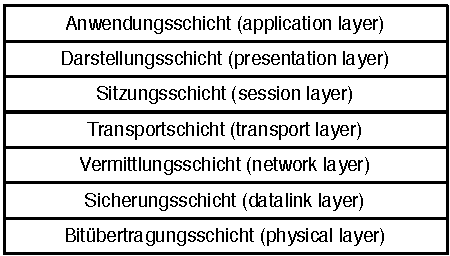
\includegraphics[bb=0bp 0bp 77mm 45mm,clip]{foundations/osi_layers}

\caption{\label{fig:osi_layers}OSI Schichtenmodell}

\end{figure}


Die Funktionen der einzelnen Schichten werden in den nachfolgenden
Abschnitten beschrieben.

Zwei Netzwerksprozesse kommunizieren so miteinander, dass jeder Prozess
-- also jedes laufende Anwendungsprogramm -- ausschlie�lich direkten
Kontakt mit der obersten Schicht -- der Anwendungsschicht -- aufnimmt.
Diese Anwendungsschicht verwendet zur weiteren Erf�llung ihrer Funktionen
die direkt darunterliegende Schicht. Jede einzelne Schicht verwendet
ihrerseits jeweils nur die direkt darunterliegende Schicht. Das wird
solange fortgef�hrt bis die unterste Schicht -- die Schicht 1 -- erreicht
ist. Diese Schicht ist die Bit�bertragungsschicht, da auf dieser Ebene
die eigentliche �bertragung der Bits in Form von Signale stattfindet.
Danach wird beim Kommunikationspartner die Hierarchie der Schichten
von unten nach oben durchlaufen. Bei der Antwort wird der gleiche
Weg zur�ckgenommen. Dieser Vorgang ist in Abbildung \vref{fig:communication_layers}
dargestellt.

%
\begin{figure}[h]
\centering

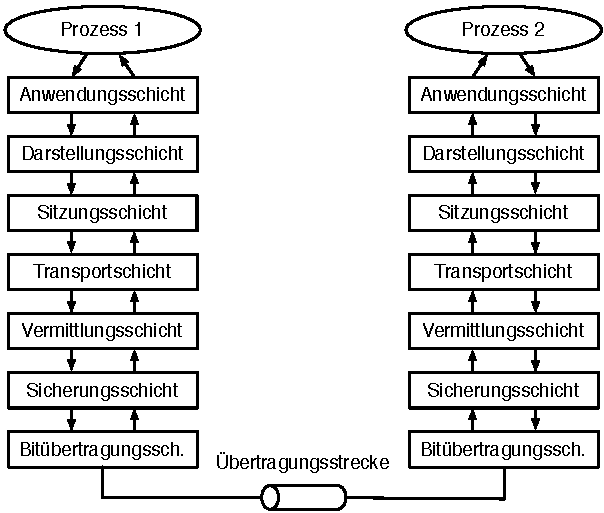
\includegraphics[bb=0bp 0bp 105mm 9cm,clip]{foundations/osi_communication}

\caption{\label{fig:communication_layers}Kommunikation zwischen den Schichten
im OSI Modell}

\end{figure}



\subsection{Protokollhierarchie\label{sec:protocol_hierarchy}}

Meistens ist es so, dass die Prozesse auf verschiedenen Knoten im
Netz laufen. Damit handelt es sich notwendigerweise auch um verschiedene
Auspr�gungen der Netzwerksoftware. Eine Schicht einer auf einem Knoten
installierten Netzsoftware wird in diesem Zusammenhang als Instanz
einer Schicht bezeichnet. In diesem Sinne kommunizieren zwei Instanzen
einer Ebene untereinander mittels eines Protokolles. Da die eigentlichen
Signale nur �ber die physikalische �bertragungsstrecke �bertragen
werden k�nnen, findet die Kommunikation -- wie oben beschrieben --
�ber den Umweg der darunterliegenden Instanzen statt. Dadurch entsteht
eine Protokollhierarchie, auch Protokollstack genannt (siehe Abbildung
\vref{fig:osi_protocol_hierarchy}).

%
\begin{figure}[h]
\centering

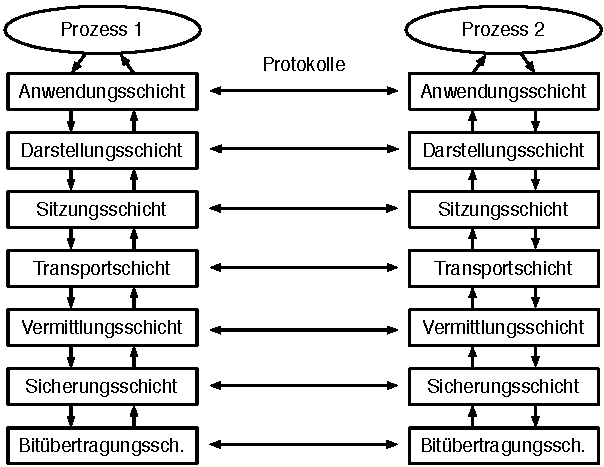
\includegraphics[bb=0bp 0bp 120mm 8cm,clip]{foundations/osi_protocol_hierarchy}

\caption{\label{fig:osi_protocol_hierarchy}Protokollhierarchie der 7 OSI Schichten}

\end{figure}


Eine beliebige benannte Schicht wird in der OSI Nomenklatur als (N)-Schicht
bezeichnet, wobei N die Werte 1 bis 7 annehmen kann.


\subsection{Nachrichten zwischen Schichten\label{sec:messages_layers}}

Die eigentliche Kommunikation wird so durchgef�hrt, dass jeder Informationsblock,
der nach unten an die unterliegende Instanz gegeben wird, in einen
Umschlag (engl. envelope) verpackt wird, der zus�tzliche Informationen
beinhaltet. Bei diesem Umschlag handelt es sich um einen Vorspann
(engl. header) und manchmal auch um einen Nachspann (engl. trailer).
Beim Prozess des Kommunikationspartners wird dieser Umschlag von der
Partnerinstanz entfernt und der so erhaltene Informationsblock an
die obenliegende Instanz weitergereicht. Der R�ckweg wird wieder analog
behandelt (siehe Abbildung \vref{fig:osi_messages_layers}).

%
\begin{figure}[h]
\centering

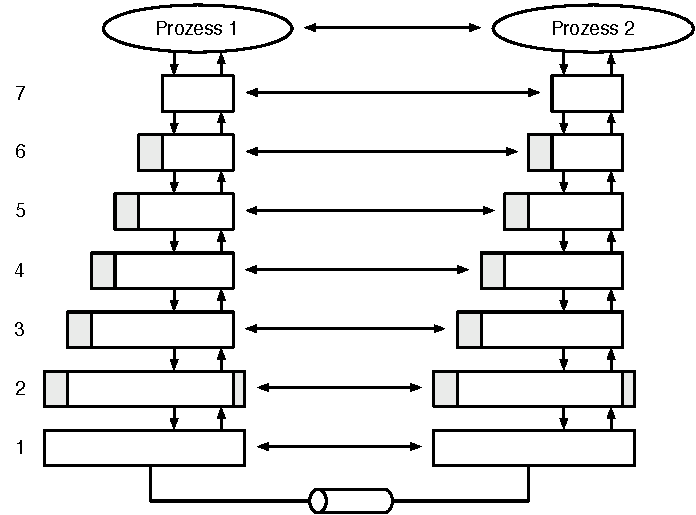
\includegraphics[bb=0bp 0bp 120mm 9cm,clip]{foundations/osi_messages_layers}

\caption{\label{fig:osi_messages_layers}Nachrichtenfluss zwischen den 7 OSI
Schichten}

\end{figure}


Die grau hinterlegten Teile der Datenbl�cke sind Teile des Umschlags.
Bei TCP/IP wird ein Trailer nur auf Schicht 2 verwendet. In Abbildung
\vpageref{fig:osi_messages_layers} wurde aus diesem Grund nur in
der Schicht 2 ein Trailer eingezeichnet.

Diese Informationsbl�cke, die zwischen den einzelnen Schichten ausgetauscht
werden, sind die eigentlichen Nachrichten, die zwischen je zwei Instanzen
einer Schicht im Zuge des gemeinsamen Protokolls ausgetauscht werden.
Dabei haben sich teilweise je nach Schicht eigene Bezeichnungen etabliert:
\begin{itemize}
\item Auf der Schicht 2 wird von einem Rahmen (engl. frame) gesprochen.
Handelt es sich um kurze Rahmen mit fester Gr��e, dann werden diese
Rahmen als Zellen (engl. cell) bezeichnet.
\item In der Schicht 3 wird von Datagrammen (engl. datagram) oder auch von
Paketen (engl. packet) gesprochen.
\item Im Kontext von TCP werden die Nachrichten Segmente (engl. segment)
genannt. Bei UDP wird ebenfalls von Datagrammen gesprochen.
\item Auf den restlichen Schichten 5 bis 7 bzw. als �berbegriff wird der
Begriff Nachricht (engl. message) verwendet.
\end{itemize}
Nachrichten im Sinne der Schichten 2-4 sind dadurch charakterisiert,
dass sie eine festgelegte maximale Gr��e aufweisen. Dadurch unterscheiden
sie sich von den Nachrichten, die direkt zwischen den Anwendungen
ausgetauscht werden, die keinerlei Einschr�nkung bzgl. der Gr��e unterliegen.


\subsection{Protokollmechanismen}

In den einzelnen Schichten gibt es Funktionen, die bzgl. einer Abstraktion
vergleichbar sind. Diese Funktionen werden als Protokollmechanismen
bezeichnet. Diejenigen Funktionen, die spezifisch f�r eine jeweilige
Schicht sind, werden dann im Abschnitt \vref{sec:osi_layers} beschrieben.


\subsubsection{Protokollauswahl}

Die Auswahl eines Protokolles (engl. protocol selection) bzw. die
Identifizierung (engl. identification) ist eine der ersten Aufgaben
beim Kommunikationsbeginn. �fters ist es so, dass zwischen zwei Kommunikationspartnern
oder spezieller in einer Schicht mehrere Protokolle zur Verf�gung
stehen. Eines dieser Protokolle muss zur Kommunikation ausgew�hlt
werden. Dazu muss es nat�rlich identifiziert, also benannt werden.

Im Laufe der Lebenszeit eines Systemes ist es sehr wahrscheinlich,
dass das Protokoll an die laufenden �nderungen angepasst werden muss
(Protokollevolution). D.h. das Protokoll wird in mehreren Versionen
vorliegen und es ist die Auswahl einer konkreten Version (engl. protocol
version selection) notwendig.

Diese Auswahl eines geeigneten Protokolles bzw. einer speziellen Version
muss zwischen den beiden Kommunikationspartnern ausgehandelt werden
(engl. negotiation mechanism).


\subsubsection{Verbindungen}

Der Aufbau einer Verbindung (engl. connection establishment), der
Transfer der Daten und der Abbau einer Verbindung (engl. connection
release) sind die grundlegenden Elemente im Lebenszyklus einer Verbindung.
Allgemein verbindet eine Verbindung zwei Kommunikationspartner, bei
denen es sich wiederum speziell um Instanzen von Schichten handeln
kann.

Eine Verbindung in einer (N)-Schicht kann mittels einer Verbindung
auf der (N-1)-Schicht oder verbindungslos auf der (N-1)-Schicht realisiert
werden. Eine verbindungslose Kommunikation auf einer (N)-Schicht kann
verbindungsorientiert oder verbindungslos mittels der (N-1)-Schicht
realisiert werden. Es ergeben sich daher 4 verschiedene M�glichkeiten.

Abweichend vom normalen Datentransfer ist es manchmal sinnvoll, Daten
vorrangig auszuliefern. Dies wird als Vorrang-Datentransfer (engl.
expedited data transfer) bezeichnet.

Zus�tzlich zum normalen Abbau einer Verbindung gibt es auch einen
speziellen Verbindungsabbruch (engl. abort). Dieser ist dadurch gekennzeichnet,
dass ausstehende �bertragungen nicht mehr durchgef�hrt werden, w�hrend
bei einem normalen Verbindungsabbau diese ausstehenden �bertragungen
sehr wohl noch durchgef�hrt werden.

Manche Dienste erfordern eine Zur�cksetzfunktion (engl. reset), die
den Dienst oder im Speziellen die Verbindung in einen vordefinierten
Zustand zur�cksetzen. Das kann notwendig werden, wenn das Protokoll
von einem Partner nicht mehr eingehalten wurde. Dadurch kann es zu
einem Verlust oder zu einer Duplizierung von Daten kommen.

D.h. man kann zwischen verbindungsorientierten (engl. connection-oriented)
und verbindungslosen (engl. connectionless) Protokollen unterscheiden:
\begin{itemize}
\item Verbindungsloses~Protokoll

\begin{itemize}
\item effizient
\item wenn Netzwerk relativ zuverl�ssig ist (wie in einem LAN), d.h. solange
Pakete nicht verloren gehen oder besch�digt werden.


Beispiel: Wenn keine Antwort kommt, dann muss z.B. der Client nochmals
schicken. Problem: ,,�berweise 10.000 Euro von meinem Konto'' sollte
nicht nochmals gesendet werden. D.h. die Anforderung nochmals zu senden
macht nur in bestimmten F�llen Sinn.

\end{itemize}
\item Verbindungsorientiertes~Protokoll

\begin{itemize}
\item Overhead, da Einrichten und Abbauen einer Verbindung relativ kostspielig
ist.
\item wenn Netzwerk nicht zuverl�ssig ist (wie in einem WAN).
\end{itemize}
\end{itemize}
Prinzipiell kann auch noch zwischen einem \emph{zustandsbehafteten}
und einem \emph{zustandslosen} Protokoll unterschieden werden. D.h.
h�ngen im Protokoll die Nachrichten vom Zustand der vorhergehend gesendeten
Nachrichten ab oder nicht.

http ist ein typisch zustandsloses Protokoll, das �ber ein verbindungsorientiertes
Transportprotokoll �bertragen wird. Man beachte die verschiedenen
Protokollhierarchieebenen, die hier eine Rolle spielen.

Eine \emph{Sitzung} (Session) ist charakterisiert, dass es
\begin{itemize}
\item eine feste Beziehung zwischen den kommunizierenden Prozessen auf Anwendungsebene
mit vereinbarten Eigenschaften (Namen, Ressourcen, Charakteristika,...)
gibt.
\item einen gemeinsamen Zustand zwischen den kommunzierenden Prozessen w�hrend
der Session gibt. 
\item meist auch Mechanismen der Authentifikation und Autorisierung gibt.
\end{itemize}
D.h. eine Session kann nur mit einem zustandsbehafteten Protokoll
aufgebaut werden. Setzt man diese Aussage in den Zusammenhang mit
Sessions im Web, dann kann man einwerfen, dass es sich bei http um
ein zustandsloses Protokoll handelt. Das ist richtig, deshalb wird
in solch einem Fall der Zustand explizit zwischen den Kommunikationspartnern
bei jedem Nachrichtenaustausch �bertragen. Oft wird jedoch nicht der
gesamte Zustand (vgl. Warenkorb) �bertragen, sondern nur eine eindeutige
Information unter der der Zustand im Server gespeichert ist.


\subsubsection{Sicherstellung einer zuverl�ssige �bertragung}

Zur Fehlererkennung (engl. error detection) und Fehlerkorrektur (engl.
error correction) gibt es verschiedene M�glichkeiten.

Ein Verlust einer Nachricht kann erkannt werden, wenn nach dem Absenden
einer Nachricht innerhalb einer vorgegebenen Zeitspanne (engl. timeout)
keine positive Quittierung (engl. acknowledgement oder kurz ACK) empfangen
wird. Ein ACK kann entweder als eigene Nachricht oder als Huckepack-Quittierung
(engl. piggy back acknowledgement) gesendet werden.

Zur Erkennung von Fehlern innerhalb einer Nachricht werden Pr�fsummen
(engl. check\-sum) herangezogen. Wird in einer Nachricht ein Fehler
erkannt, dann gibt es die folgenden M�glichkeiten: 
\begin{itemize}
\item Die Nachricht wird verworfen.
\item Die Nachricht wird verworfen und es wird eine negative Quittierung
(engl. negative acknowledgment oder kurz NACK) gesendet.
\item Die Nachricht kann automatisch korrigiert werden.
\end{itemize}
Allgemein: Die positive Quittierung dient als Best�tigung f�r das
Erreichen eines bestimmten Zustandes. Bei Nichterreichen eines bestimmten
Zustandes kann analag dazu eben eine negative Quittierung gesendet.

Damit die Reihenfolge der Nachrichten innerhalb eines Protokolle sichergestellt
werden kann, werden Sequenznummern verwendet (engl. sequencing). Diese
Sequenznummern werden auch bei der Anpassung der Systemleistung (siehe
Abschnitt \vref{sec:performance_system}) verwendet.


\subsubsection{Anpassung an die L�nge\label{sec:segmenting}}

Wie in schon Abschnitt \ref{sec:messages_layers} beschrieben ist
es oft so, dass die maximale Gr��e einer Nachricht je Schicht unterschiedlich
sein kann. Dadurch ergibt sich die Notwendigkeit die Gr��en der Nachrichten,
die zwischen einer (N)-Schicht und der (N-1)-Schicht ausgetauscht
werden anzupassen.

Den Vorgang des Aufteilens einer Nachricht auf mehrere Nachrichten
geringerer Gr��e zum Zwecke der Anpassung an die geringere maximale
Gr��e der anderen Schicht nennt man Segmentierung (engl. segmenting).
Den umgekehrten Vorgang des Zusammensetzens mehrere kleinerer Nachrichten
zu einer gr��en Nachricht nennt man Reassemblierung (engl. reassembling).


\subsubsection{Anpassung an die Systemleistung\label{sec:performance_system}}

Der Empf�nger von Nachrichten muss vor einer �berlastung durch den
Sender gesch�tzt werden. Dies nennt man \emph{Flusskontrolle} (engl.
flow control).

Der Schutz eines Netzes vor �berlastung durch die von allen Sendern
gesendeten Nachrichten nennt \emph{�berlaststeuerung} (engl. congestion
control).


\subsubsection{Anpassung der �bertragungsleistung}

Will man eine �bertragungsleistung einer Verbindung mehreren Kommunikationspartner
zur Verf�gung stellen, spricht man von Multiplexen (engl. multiplexing).
D.h. allgemein wird eine (N-1)-Verbindung -- eine Verbindung in einer
(N-1)-Schicht -- f�r mehrere (N)-Verbindungen nutzbar gemacht. Den
analogen Vorgang die (N-1)-Verbindung wieder auf die (N)-Verbindungen
aufzuteilen hei�t Demultiplexen (engl. demultiplexing).

Wird allerdings eine �bertragungsleistung gefordert, die nicht durch
eine Verbindung der unterliegenden Schicht erf�llt werden kann, dann
m�ssen mehrere Verbindungen dieser untenliegenden Schicht verwendet
werden. Dazu wird eine (N)-Verbindung auf mehrere (N-1)-Verbindungen
aufgeteilt (engl. splitting) und beim Empf�nger werden analog dazu
die (N-1)-Verbindungen wieder zu der (N)-Verbindung zusammengesetzt
(engl. recombining).


\subsubsection{Dienstg�te}

Die Verhandlung einer bestimmten Dienstg�te (engl. quality of service
oder kurz QoS) fasst alle Parameter zusammen, die eine Verbindung
oder eine einzelne Nachrichten�bermittlung betreffen. Diese Parameter
werden beim Aufbau der Verbindung ausverhandelt (verbindungsorientiert)
oder bei jeder einzelnen Nachrichten�bermittlung (verbindungslos).
D.h. der Sender fordert Parameter an, die der Empf�nger voll oder
teilweise akzeptiert.

Beispiele f�r solche Parameter (nach Attributen aufgeschl�sselt):
\begin{description}
\item [{Leistung}]~

\begin{description}
\item [{Durchsatz}] Unter dem Durchsatz (engl. throughput) wird die zugesicherte
Menge an Benutzerdaten pro Zeiteinheit verstanden, die �bertragen
werden.
\item [{�bertragungsverz�gerung}] Die �bertragungsverz�gerung (engl. transmission
delay, latency) gibt die maximale Zeitdauer zwischen dem Absenden
der Anfrage und der Ankunft beim Emf�nger an.
\item [{Schwankung~der~�bertragungsverz�gerung}] (engl. jitter) ist die
Varianz der Latenzzeit von Datenpaketen. Dieser Effekt ist insbesondere
bei Multimedia-Anwendungen (zum Beispiel Audio-Streaming und IP-Telefonie)
unerw�nscht.
\item [{Verbindungaufbauverz�gerung}] (engl. connection establishment delay)
beschreibt die maximale Zeit die vergeht bis eine Verbindung aufgebaut
ist.
\item [{Verbindungsbeendigungsverz�gerung}] (engl. connection release delay)
analog zur Verbindungsaufbauverz�gerung.
\item [{Priorit�t}] Die Priorit�t (engl. priority) des Datentransfers gibt
an inwieweit vorrangig Daten �bertragen werden k�nnen.
\end{description}
\item [{Zuverl�ssigkeit}]~

\begin{description}
\item [{Vollst�ndigkeit}] Angabe inwieweit eine Zusicherung gegeben werden
kann, dass die Nachrichten zumindest einmal beim Kommunikationspartner
ankommen bzw. inwieweit es zu Verlust von Nachrichten kommt (engl.
probability of loss).
\item [{Fehlerraten}] Wahrscheinlichkeit der Datenver�nderung (engl. probability
of corruption).
\item [{Eindeutigkeit}] Vermeidung der Duplizierung von Nachrichten (engl.
probability of duplication).
\item [{Reihenfolge}] Einhaltung der Reihenfolge der Nachrichten (engl.
probability of out of sequence delivery).
\item [{Garantien}] Angabe inwieweit die Leistungsparameter erbracht werden
k�nnen. Das meist genutzte Prinzip ,,best effort'' gibt lediglich
an, dass die Werte so gut wie m�glich eingehalten werden, aber keine
Garantie angegeben werden kann. Andere Angaben werden oft mit Wahrscheinlichkeiten
beziffert, sofern andere Bedingungen -- wie z.B. funktionierende Software
und Hardware -- erf�llt sind.
\end{description}
\item [{Sicherheit}] Darunter werden alle Ma�nahmen angegeben, die die
Sicherheit der Kommunikation sicherstellen k�nnen (siehe Teil \ref{par:security}).
\end{description}

\subsection{Schichten\label{sec:osi_layers}}


\subsubsection{Schicht 1 -- Bit�bertragungsschicht}

In der Bit�bertragungsschicht (engl. physical layer) werden die physikalischen
Eigenschaften der �bertragungsstrecke beschrieben. Dies inkludiert
das �bertragungsmedium (siehe Abschnitt \vref{sec:transmission_media})
wie z.B. ein Kabel, das �bertragungsverfahren (siehe Abschnitt \vref{sec:transmission_methods})
und den �bergang auf das �bertragungsmedium wie z.B. Steckverbindungen.
Im Detail handelt es sich um die elektrischen, mechanischen, optischen
oder elektromagnetischen Spezifikationen.

Als Erweiterung zum OSI Modell kann die Bit�bertragungsschicht noch
weiter unterteilt werden in:
\begin{itemize}
\item Media~Independent~Interface (abgek�rzt mit MII), bietet die einheitliche
unterschiedlicher �bertragungsmedien.
\item Physical~Media~Dependent (abgek�rzt mit PMD) ist f�r den eigentlichen
Zugriff auf das �bertragungsmedium zust�ndig. Z.B. kann als �bertragungsmedium
entweder eine verdrillte Zweitdrahtleitung oder ein Koaxialkabel verwendet
werden.
\end{itemize}

\subsubsection{Schicht 2 -- Sicherungsschicht }

Die Hauptaufgabe der Sicherungsschicht (engl. data link layer) liegt
in der fehlerfreien Punkt-zu-Punkt �bertragung ganzer Rahmen zwischen
\emph{benachbarten Stationen}. Diese Stationen k�nnen entweder direkt
miteinander oder �ber einen Bus verbunden sein.

Im Falle eines Bussystems muss jeder Knoten auch eine eigene Adresse
haben, die MAC-Adresse (engl. media access control) genannt wird.
Es handelt sich dabei um eine Hardwareadresse, die direkt dem Netzwerkadapter
des Knotens zugeordnet ist. Als solches muss diese MAC-Adresse zumindest
innerhalb des Bussystems eindeutig sein. H�ufig sind diese MAC-Adressen
jedoch global eindeutig vergeben (siehe Abschnitt \vref{sec:ethernet}).

Als Erweiterung zum OSI Modell kann die Sicherungsschicht noch weiter
unterteilt werden:
\begin{description}
\item [{Logical~Link~Control}] (abgek�rzt mit LLC), die die eigentlichen
Funktionen der Schicht 2 abdeckt.
\item [{Media~Access~Control}] (abgek�rzt mit MAC), die den Zugriff auf
das �bertragungsmedium steuert.
\end{description}

\subsubsection{Schicht 3 -- Vermittlungsschicht}

In der Vermittlungsschicht oder auch Netzwerksschicht (engl. network
layer) genannt werden haupts�chlich die Nachrichten weitervermittelt.
Die �bertragung geht �ber das gesamte Netzwerk hinweg und schlie�t
das Weiterleiten zwischen den Netzknoten mit ein. D.h. eine Nachricht
wird von einem (End-)Knoten -- unter Umst�nden �ber mehrere Zwischenknoten
hinweg -- zu einem anderen (End-)Knoten �bermittelt (Ende-zu-Ende,
engl. end-to-end). Ebenfalls auf dieser Ebene sind die Netzadressen
angesiedelt, die �ber das gesamte Netz eindeutig vergeben werden m�ssen.


\subsubsection{Schicht 4 -- Transportschicht}

Die Transportschicht (engl. transport layer) stellt Verbindungen zwischen
den kommunizierenden Netzprozessen als Ende-zu-Ende Verbindungen zur
Verf�gung. D.h., dass auf dieser Ebene wird einerseits das Konzept
der Verbindungen und andererseits werden Mechanismen f�r eine Adressierung
der Netzprozesse als Kommunikationspartner zur Verf�gung gestellt.
Wie schon erw�hnt beinhaltet das Konzept der Verbindung auch, dass
Nachrichten vollst�ndig, fehlerfrei, in der richtigen Reihenfolge
und genau einmal beim Empf�nger eintreffen. Daf�r ist ebenfalls die
Transportschicht zust�ndig.


\subsubsection{Schicht 5 -- Sitzungsschicht}

In der Sitzungsschicht (engl. session layer) wird die Steuerung der
Kommunikation zwischen den kommunizierenden Netzprozessen gesteuert.
Sie unterst�tzt eine Dialogsteuerung, um zu verfolgen welche Partei
gerade spricht und stellt Funktionen f�r die Synchronisierung bereit.
Dazu wird ebenfalls eine Verbindung auf dieser Ebene realisiert, die
auch Wiederaufsetzpunkte (engl. check point) einsetzt, um die Kommunikation
bei einem Synchronisationsverlust zwischen Sender und Empf�nger wieder
kontrolliert fortsetzen zu k�nnen.


\subsubsection{Schicht 6 -- Darstellungsschicht}

Die Darstellungsschicht (engl. presentation layer) ist f�r die korrekte
Umwandlung unterschiedlicher Datenformate (z.B. ASCII in UTF-8, little-endian
in big-endian oder allgemeine Umwandlung von Zahlendarstellungen)
zust�ndig. Ebenfalls z�hlen Datenkompression und Verschl�sselung zu
den Aufgaben dieser Ebene.


\subsubsection{Schicht 7 -- Anwendungsschicht}

Als oberste Schicht im OSI Modell stellt die Anwendungsschicht (engl.
application layer) die Schnittstelle zum Netzprozess dar. Die Aufgaben
dieser Schicht liegen im Bereitstellen von Diensten, die oft von Netzprozessen
ben�tigt werden, wie z.B. Daten�bertragung, E-Mail, oder entferntes
Anmelden (engl. remote login).



\chapter{Nachrichten�bertragung}

Dieser Abschnitt erl�utert die Grundlagen zur Nachrichten�bertragung
zwischen \emph{zwei} Kommunikationspartnern, die \emph{direkt} physikalisch
�ber ein Medium oder logisch �ber einen Kanal miteinander verbunden
sind (Punkt-zu-Punkt Verbindung).

In diesem Kapitel werden einerseits die allgemeinen Aspekte einer
Nachrichten�bertragung bei einer Punkt-zu-Punkt Verbindung behandelt,
aber auch die spezielle Kommunikation �ber eine physikalische �bertragungsstrecke.


\section{Kommunikationsmodell\label{sec:communication_model}}

Ein allgemeines Kommunikationsmodell, das dann nat�rlich auch f�r
eine physikalische Punkt-zu-Punkt Verbindung gilt sieht folgenderma�en
aus:

%
\begin{figure}[H]
\centering

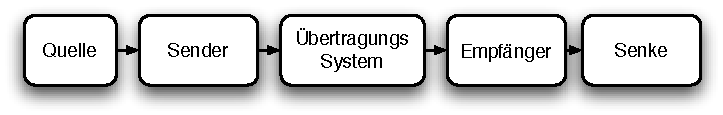
\includegraphics[bb=0bp 0bp 128mm 19mm,clip]{transmission/communication_model}

\caption{Kommunikationsmodell}

\end{figure}

\begin{description}
\item [{Quelle}] (engl. source) Die (Informations-)Quelle erzeugt die zu
�bertragenden Nachrichten.
\item [{Sender}] (engl. transmitter) Der Sender nimmt von der Quelle die
Nachrichten entgegen, kodiert diese und wandelt sie in Signale um.
Danach werden diese gem�� den Zugriffsregeln dem �bertragungssystem
zum Transport �bergeben.
\item [{�bertragungssystem}] (engl. transmission System) Im eigentlichen
�bertragungssystem (oder auch �bertragungsstrecke genannt) werden
die Signale �bertragen. Im einfachsten Fall handelt es sich beim �bertragungssystem
um eine elektrische Leitung �ber die elektrische Signale �bertragen
werden, im allgemeinen Fall jedoch um ein komplettes Netzwerk (siehe
Kapitel \vref{sec:network_architecture}).
\item [{Empf�nger}] (engl. receiver) Am anderen Ende wandelt der Empf�nger
die Signale wieder in Nachrichten um, die entsprechend dekodiert an
die Senke weitergegeben werden. Im Prinzip besteht ein Empf�nger aus
einem Signalumsetzer und einer Fehlersicherungseinrichtung.
\item [{Senke}] (engl. destination) Die (Informations-)Senke empf�ngt die
Nachrichen und verarbeitet diese.
\end{description}
Sowohl Quelle als auch Senke werden aus der Sicht eines verteilten
Systems als Netzprozess oder kurz Prozess betrachtet. Unter einem
Prozess versteht man die Ausf�hrung von einem Progamm. Zwei solcher
Prozesse sind logisch �ber einen (Kommunikations-) Kanal miteinander
verbunden. Die Rollen der Quelle und der Senke k�nnen nat�rlich dynamisch
tauschen.

Technisch gesehen l�sst sich das Kommunikationsmodell f�r eine physikalische
Verbindung folgenderma�en abbilden:

%
\begin{figure}[H]
\centering

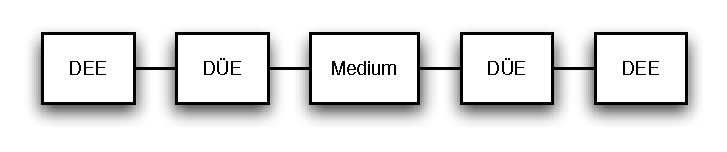
\includegraphics[bb=0bp 0bp 126mm 22mm,clip]{transmission/data_transmission}

\caption{Daten�bertragung}

\end{figure}


Unter der Datenendeinrichtung (DEE oder engl. Data Terminal Equipment,
DTE) wird sowohl die Quelle der Information als auch die Senke verstanden.
Im Falle der Rechnernetze handelt es sich dabei um die Rechner, die
auch als Hosts bezeichnert werden. Unter einer Daten�bertragungseinrichtung
(D�E oder engl. Data Communications Equipment, DCE) werden die Ger�te
verstanden, die die Transmitter bzw. die Receiver darstellen. Beispiele
f�r solche D�E sind z.B. Modems (MODulator/DEModulator) oder die Netzwerksschnittstellenkarten
(Network Interface Card - NIC).


\section{�bertragungsmedien\label{sec:transmission_media}}

Dieser Abschnitt betrachtet jetzt speziell die verschiedenen Arten
von �bertragungsmedien, die in Rechnernetzen eingesetzt werden. Prinzipiell
erfolgt die �bertragung in einer von zwei Formen:
\begin{itemize}
\item leitungsgebunden d.h. entweder �ber metallische Leiter wie z.B. bei
den Ethernet Technologien oder optische Fasern wie z.B. bei FDDI.
\item leitungsungebunden d.h. mittels elektromagnetischer Wellen wobei als
�bertragungsmedium die Luft dient. Hier haben sich folgende Spezialformen
etabliert:

\begin{itemize}
\item ungerichtete �bertragung wie z.B. beim Einsatz von Technologien im
terrestrischen Funk wie Wireless LAN, Bluetooth, GSM, UMTS.
\item gerichtete �bertragung wie z.B. beim Richtfunk, der Satellitenkommunikation
oder auf Basis optischer Signale wie z.B. Infrarot�bertragung.
\end{itemize}
\end{itemize}
Je nach �bertragungsmedium werden zus�tzlich entweder Steckverbindungen,
Antennen oder andere �bertragungsglieder ben�tigt, um den �bergang
des Signals auf das �bertragungsmedium durchzuf�hren.


\subsection{Metallische Leiter}

Es werden entweder symmetrische Kupferkabel oder Koaxialkabel eingesetzt.
Bei Verwendung metallischer Leiter kommen heute nur mehr symmetrische
Kupferkabel zum Einsatz.


\subsubsection{Symmetrische Kupferkabel}

Diese Form der Kupferkabel verwendet ein oder mehrere verdrillte Paare
von Kupferadern. Aus diesem Grund werden diese Kabel auch als Twisted
Pair (TP) bezeichnet. Der Aufbau der Kabelbezeichnungen ist nach ISO/IEC-11801:2002
folgenderma�en XX/YZZ wobei XX die Angabe der Kabelabschirmung darstellt
und entweder
\begin{labeling}{00.00.0000}
\item [{U}] unshielded, d.h. ohne Abschirmung des gesamten Kabels,
\item [{S}] screened, d.h. Abschirmung des gesamten Kabels mittels Drahtgeflecht,
\item [{F}] foiled, d.h. Abschirmung des gesamten Kabels mittels Folie,
\item [{SF}] screened, foiled, d.h. Abschirmung des gesamten Kabels mittels
Drahtgeflecht und Folie
\end{labeling}
annehmen kann. Y steht f�r die Abschirmung der einzelnen Aderpaare
und kann die Werte
\begin{labeling}{00.00.0000}
\item [{U}] unshielded, d.h. keine Abschirmung der einzelnen Aderpaare,
\item [{S}] shielded, d.h. Abschirmung der einzelnen Aderpaare mittels
Drahtgeflecht,
\item [{F}] foiled, d.h. Abschirmung der einzelnen Aderpaare mittels Folie
\end{labeling}
annehmen. ZZ ist immer TP (also Twisted Pair). In der Abbildung \vref{fig:twisted_pair_cable}
ist ein 4 adriges TP Kupferkabel schematisch dargestellt.

%
\begin{figure}[h]
\centering

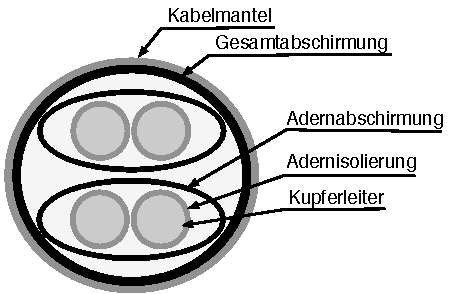
\includegraphics[bb=0bp 0bp 8cm 5cm,clip]{transmission/cable}

\caption{\label{fig:twisted_pair_cable}TP Kupferkabel mit 4 Adern}

\end{figure}


In der ISO/IEC Spezifikation 11801 werden au�erdem sogenannte Linkklassen
definiert, die die Qualit�t einer gesamten �bertragungsstrecke inkl.
Kabel und Steckverbindungen angeben. Es gibt die Linkklassen A bis
F, in denen die notwendigen elektrischen Parameter definiert sind,
die f�r den Einsatz von bestimmten Anwendungen -- wie z.B. 100MBit
Ethernet oder Gigabit-Ethernet -- ben�tigt werden.

Je Linkklasse k�nnen verschiedene Kabeltypen eingesetzt werden. Die
Kabeltypen werden in sogenannte Kategorien eingeteilt, wobei die Kategorien
von 1 bis 7 durchnummeriert werden. F�r jeden Kabeltyp sind wieder
verschiedene elektrische Parameter festgelegt.

Aus der Kombination von Linkklasse und Kabeltyp ergeben sich �berbr�ckbare
Distanzen. Im LAN werden derzeit haupts�chlich Kategorie 5 (Cat-5)
Kabel eingesetzt, die eine 100MBit Ethernet Verbindung �ber 100m erlauben.
Mit einem Cat-5 Kabel bestehend aus 4 Doppeladern kann auch eine Gigabit
Ethernet Verbindung in beide Richtungen aufgebaut werden. F�r 10 Gigabit
Ethernet muss allerdings ein Kabeltyp h�herer Kategorie verwendet
werden.

Zu dem Kabel passend m�ssen auch die Steckverbindungen ausgef�hrt
sein. Als Steckverbindungen werden heute meist die 8 poligen RJ-45
Stecker verwendet.

Die Vorteile der Twisted-Pair Kabel liegen darin, dass die Verlegung
relativ einfach ist, die Kosten gering sind, eine weite Anwendbarkeit
besteht und die Verbreitung sehr hoch ist.


\subsubsection{Koaxialkabel\label{sec:coaxial_cable}}

Koaxialkabel bestehen gew�hnlich aus einem isolierten Innenleiter
(auch Seele genannt), der vom Au�enleiter umgeben ist. Dieser Au�enleiter
ist in einem konstanten Abstand um den Innenleiter angebracht und
von diesem durch einen Isolator getrennt. Im Regelfall ist diese Ummantelung
ebenfalls nach au�en isoliert. Solch ein in Rechnernetzen eingesetztes
Koaxialkabel �hnelt dem Fernsehkabel.

Das Koaxialkabel wurde fr�her in Ethernet Rechnernetzen verwendet.
Dazu wurden haupts�chlich 2 Kabeltypen eingesetzt: Eines f�r die Ethernet
Spezifikation 10Base5 und eines f�r die Ethernet Spezifikation 10Base2.

10Base5 (Thicknet oder Yellow Cable genannt) verwendete ein 10mm dickes
Koaxialkabel. Die Verbindungen wurden mittels Anbohren des Kabels
(im Abstand von min. 2.5m) und Anklemmen eines Transceivers, der �ber
eine AUI (engl. access unit interface) Schnittstelle die Verbindung
zum Ethernet-Controller herstellte.

10Base2 (Thinnet genannt) verwendete ein ca. 6mm dickes Koaxialkabel.
Zur Verbindung wurden allerdings BNC (engl. bayonet Neill-Concelman)
Stecker verwendet.

Koaxialkabel werden heutzutage nicht mehr oft verwendet.


\subsection{Optische Leiter}

Die optischen Leiter (engl. optical fiber) bestehen aus einem Kern
(engl. core) und einem Mantel (engl. cladding). Das Lichtsignal wird
in den Kern �ber eine Photodiode oder eine Laserdiode eingespeist.
Da der Brechungsindex des Mantels niedriger ist als der des Kerns
kommt es zu einer Reflexion am �bergang von Kern zu Mantel, wodurch
sich das Lichtsignal im Kern zickzackf�rmig ausbreitet.

Es werden im Wesentlichen zwei Typen von Glasfasern unterschieden:
dies sind die Multimodefasern und die Single- bzw. Monomodefasern.
Multimodefaser haben einen Durchmesser des Kernes von 50$\mu m$ oder
62.5$\mu m$, w�hrend Singlemodefasern einen Kerndurchmesser von ca.
3 bis 9$\mu m$ haben.

Auf Grund des relativ hohen Durchmessers der Multimodefasern wird
das Licht in mehreren Wellen (Moden) �bertragen. Dadurch kann es bei
der Multimode�bertragung allerdings zu Signalbeeinflussungen kommen.
Daher sind Multimodefasern f�r sehr lange �bertragungsstrecken bei
hoher Bandbreite nicht geeignet. Bei der Singlemodefaser kann sich
das Licht auf Grund des kleinen Kerndurchmessers nahezu geradlinig
in einer Mode ausbreiten. D.h. es kommt zu keinen Signalbeeinflussungen
und zu einer geringeren D�mpfung. Unter D�mpfung versteht man die
Umwandlung von Schwingungsenergie in eine andere Energieform, d.h.
es kommt zu einer Verminderung der �bertragenen Energie im Verlauf
einer �bertragungsstrecke. Dadurch lassen sich h�here Entfernungen
bei gr��erer Bandbreite als bei den Multimodefasern �berbr�cken.

Optische Leiter zeichnen sich -- abgesehen von der h�heren Bandbreite
bei gr��erer Entfernung -- durch geringere St�rempfindlichkeit und
h�here Abh�rsicherheit aus. Allerdings ist die Verlegung schwieriger
und die Kosten sind h�her.


\subsection{Funk\label{sec:wireless_transmission}}

Die �bertragung basiert darauf, dass hochfrequente Wellen (800MHz
bis mehrere GHz) �ber das �bertragungsmedium Luft gesendet werden.
Besonders in LANs oder auch in PANs (siehe Seite \pageref{min:net_dimensions})
werden h�ufig Netzwerke mittels Funktechnologie aufgebaut, aber auch
die Abdeckung �ber immer gr��ere geographische Gebiete wie ganze St�dte
wird aktuell. Der gro�e Vorteil liegt in der Einfachheit und Flexibilit�t
sowie in der leichten Wartbarkeit der Netze. Ebenfalls ein gro�er
Vorteil liegt in der Mobilit�t. Ein drahtloser �bertragungskanal besitzt
die Broadcast-Eigenschaft.

Funk�bertragung hat mit vielen Problemen zu k�mpfen:
\begin{itemize}
\item Es treten St�rungen und Interferenzen auf. Die Qualit�t des �bertragungskanals
�ndert sich mit der Zeit.
\item Das �bertragungsmedium muss mit anderen Kommunikationsteilnehmern
geteilt werden. Unter Umst�nden handelt es sich um ,,ungew�nschte''
Sender.
\item Es gibt viele Regulierungen (speziell bei der Frequenzvergabe) seitens
nationaler Anforderungen. Daher ist die �bertragungskapazit�t beschr�nkt,
da freie Frequenzbereiche nicht einfach zu finden sind.
\item Auf Grund des einfachen Zugriffes auf das Medium Luft treten Sicherheitsprobleme
auf.
\end{itemize}
Gegen�ber der leitungsgebundenen �bertragung ergeben sich niedrigere
�bertragungsraten im Bereich von 1 bis 54MBit/s. Neuere Entwicklungen
gehen bis 540MBit/s.


\section{�bertragungsverfahren\label{sec:transmission_methods}}

In diesem Abschnitt wird zuerst etwas n�her auf Signale eingegangen,
danach wird besprochen wie die Kodierung der Signale durchgef�hrt
werden kann und zum Schluss wie mehrere Signale �ber eine �bertragungsstrecke
mittels Multiplexen �bertragen werden k�nnen.


\subsection{Signal}

Wie schon in Abschnitt \vref{sec:communication} angesprochen, werden
Nachrichten auf pyhsikalischer Ebene in Form von Signalen (elektrisch,
optisch, Funk) �ber ein �bertragungsmedium versendet. Ein Signal ist
die physikalische Darstellungsform einer Nachricht und besteht aus
einer diskreten oder kontinuierlichen Folge von Werten eines Signalparameters
(z.B. ein Spannungswert, Stromwert oder Feldst�rke) �ber die Zeit.


\minisec{Signalarten}

Signale k�nnen bez�glich Wertevorrat oder Zeit entweder kontinuierlich
oder diskret sein.
\begin{description}
\item [{zeitkontinuierlich}] Werte eines Signals k�nnen zu jedem beliebigen
Zeitwert innerhalb eines Zeitintervalls auftreten.
\item [{zeitdiskret}] Werte eines Signals k�nnen nur zu bestimmten Zeitwerten
eines Zeitintervalls auftreten. Diese Zeitwerte sind oft innerhalb
des Zeitintervalls �quidistant.
\item [{wertkontinuierlich}] Werte des Signals k�nnen jeden beliebigen
Wert innerhalb des Werte\-intervalls annehmen.
\item [{wertdiskret}] Werte des Signals k�nnen nur bestimmte Werte des
Werteintervalls annehmen. 
\end{description}
Daraus ergeben sich 4 M�glichkeiten:
\begin{itemize}
\item zeitdiskret und wertdiskret: Man spricht von digitalen Signalen. Kommen
genau zwei diskrete Werte im Wertebereich des digitalen Signales vor,
dann spricht man von einem bin�ren Signal. Oft werden die Begriffe
digital und bin�r synonym verwendet.
\item zeitdiskret und wertkontinuierlich.
\item zeitkontinuierlich und wertdiskret.
\item zeitkontinuierlich und wertkontinuierlich: analoge Signale.
\end{itemize}

\minisec{Signalverarbeitung und Signal�bertragung}

Analoge Signale treten auf, wenn z.B. ein Audio- oder Videosignal
vorliegt. Analoge Signale m�ssen in digitale Signale transformiert
werden, damit sie in einem Rechner verarbeitet werden k�nnen. Dazu
dienen Analog/Digital Wandler. Diese tasten das analoge Signal zu
diskreten Zeitpunkten ab und ermitteln zu diesem Zeitpunkt einen diskreten
Wert des Signalparameters.

Danach wird das Signal kodiert und kann entweder verarbeitet oder
�bertragen werden. Eine �bertragung findet entweder im Basisbandbereich
oder im Breitbandbereich statt.

Unter dem Begriff Basisband (engl. baseband) versteht man denjenigen
Frequenzbereich, in dem sich das zu �bertragende Nutzsignal befindet.
In der Regel hat ein Basisbandsignal daher einen Frequenzbereich von
0 bis f$_{\text{max}}$Hz. Bei der analogen Telefonie beispielsweise
ist das Frequenzband der Bereich von 300 bis 3400 Hz.

Unter Breitband (engl. broadband) wird speziell bei der Daten�bertragung
ein Verfahren verstanden, bei dem die digitalen Signale -- im Unterschied
zum Basisbandverfahren -- nicht direkt �bertragen werden, sondern
auf ein oder mehrere hochfrequente Tr�gersignale aufmoduliert werden
(Modulation). Damit gibt es bei einem Breitbandsignal einen Frequenzbereich
von f$_{\text{min}}$ bis f$_{\text{max}}$. Breitband wird jedoch
oft auch mit einer hohen Bandbreite gleichgesetzt oder in der Bedeutung
verwendet, dass es sich um eine schnelle Daten�bertragung handelt.

Allgemein ist die Modulation die �nderung von Signalparametern (Amplitude,
Frequenz, Phase,\ldots{}) eines Tr�gersignals durch ein modulierendes/aufgepr�gtes
Signal. Bei der Demodulation wird das urspr�ngliche Signal wieder
zur�ckgewonnen. Gr�nde daf�r liegen z.B. in der Mehrfachbenutzung
des �bertragungssystems (z.B. Frequenzmultiplex, siehe Abschnitt \vref{sec:synchronous_multiplex})
oder einer besseren �bertragung und Filterung hochfrequenter Signale
(Basisband�bertragung nur �ber elektrische Leitungen).

Nachdem das Signal �bertragen worden ist, wird es unter Umst�nden
wieder dekodiert, in ein analoges Signal gewandelt und ausgegeben
(z.B. Fernseher, Lautsprecher).

Das gesamte Modell der Signalverarbeitung und Signal�bertragung l�sst
sich folgenderma�en darstellen:

%
\begin{figure}[H]
\centering

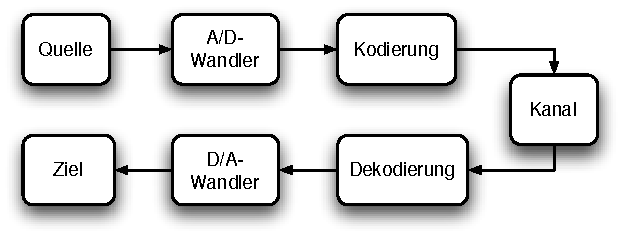
\includegraphics[bb=0bp 0bp 105mm 40mm,clip]{transmission/signal_model}

\caption{Signalverarbeitung und Signal�bertragung}

\end{figure}



\subsection{Kodierung\label{sec:coding}}

siehe Foliensatz!

\subsection{Multiplexverfahren\label{sec:multiplex}}

Unter Multiplexen (w�rtlich: mehrfach) versteht man das Konzept der
gemeinsamen Nutzung einer Systemressource durch mehrere Nutzer. Der
Grund f�r Multiplexen liegt einerseits in der wirtschaftlichen Nutzung
einer Ressource und andererseits in der Anforderung eine gewisse Form
der Nebenl�ufigkeit zu erzeugen. Das bedeutet, dass mehrere Nutzer
die Systemressource gewisserma�en gleichzeitig nutzen. Ein bekanntes
Beispiel sind die Betriebssystemprozesse, die vom Scheduler des Betriebssystems
in einem Multiplexverfahren dem Prozessor (die Systemressource) zugeteilt
werden.

Betrachtet man den Begriff Ressource, der im Sinne der Rechnernetze
und der �bertragung von Nachrichten eine Rolle spielt, dann handelt
es sich bei der Ressource um konkrete �bertragungskan�le.

Im Kontext der �bertragungstechnik kann folgende Unterteilung der
Multiplexverfahren getroffen werden.


\subsubsection{Raummultiplex\label{sec:space_division_multiplex}}

Das Raummultiplex (engl. space division multiplexing) wird auch Space
Division Multiple Access (SDMA) genannt. Die Signale werden dabei
�ber r�umlich verschiedene -- also mehrfache ($\rightarrow$ multiplex)
-- �bertragungswege �bertragen. Sollen n Signale �bertragen werden,
dann werden n Leitungen verwendet. Das analoge Telefonnetz mit der
Leitungsvermittlung kann in diese Kategorie eingeordnet werden.


\subsubsection{Synchrones Multiplex\label{sec:synchronous_multiplex}}

Die hier angef�hrten Multiplexverfahren werden deshalb als ,,synchron''
bezeichnet, da die einzelnen Signale jeweils die gleichen (oder zumindest
konstante) Anteile der �bertragungskapazit�t zur Verf�gung gestellt
bekommen.
\begin{description}
\item [{Frequenzmultiplex}] Es werden beim Frequenzmultiplexverfahren (engl.
frequency division multiplexing, FDM) die einzelnen Signale auf Tr�ger
unterschiedlicher Frequenz aufmoduliert. Die (lineare) Summe dieser
modulierten Signale wird �bertragen.
\item [{Codemultiplex}] Beim Codemultiplex (engl. code division multiplexing,
CDM) wird jedes Bit mit einer Symbolfolge, die Code genannt wird,
multipliziert. Die Codes sind zu einander orthogonal und jeder Sender
erh�lt einen solchen Code. Die, sich so ergebenen Signale werden gleichzeitig
auf dem �bertragungskanal im gleichen Frequenzband �bertragen. Solange
Empf�nger mit dem Sender zeitlich synchronisiert sind, kann der Empf�nger
das empfangene Signal wieder mit einem einzelnen Code multiplizieren
und erh�lt das einzelne Bit wieder zur�ck. Es ist ein aufw�ndiges
Verfahren, das z.B. bei UMTS verwendet wird.
\item [{Synchrones~Zeitmultiplex}] (engl. synchronous time division multiplexing,
STDM oder STM) Es wird ein Rahmen (engl. frame) mit einer festgelegten
Dauer definiert. Dieser Frame wird in Zeitschlitze (engl. time slots)
unterteilt, die den einzelnen Signalen zugeordnet werden. Solche Frames
werden nacheinander �ber den �bertragungskanal �bertragen.
\end{description}

\subsubsection{Asynchrones Zeitmultiplex\label{sec:asynchronous_multiplex}}

Das asynchrone Zeitmultiplexverfahren (engl. asynchronous time division
multiplexing, ATDM oder ATM) wird auch als statistisches Multiplexen
bezeichnet. Im Prinzip funktioniert es wie STM, jedoch erhalten nur
diejenigen Signale einen Zeitschlitz, die auch etwas zu �bertragen
haben. Dieses Verfahren hei�t deshalb auch statistisches Multiplexen,
weil die verf�gbare �bertragungskapazit�t im statistischen Mittel
besser ausgenutzt wird. Damit allerdings ein Zeitschlitz einem Signal
zugeordnet werden kann, muss eine Zuordnung im Zeitschlitz mit�bertragen
werden. Diese Zuordnung wird in der Regel mit einem Header durchgef�hrt,
der am Anfang eines Zeitschlitzes �bertragen wird. Dadurch entsteht
ein gewisser Overhead.

Das asynchrone Zeitmultiplexverfahren wird au�er in der �bertragungstechnik
bei der Entwicklung von Kommunikationsprotokollen eingesetzt! Damit
ist es das wichtigste Multiplexverfahren, das f�r den Entwickler von
verteilten Systemen eine Rolle spielt.


\section{Sicherungsverfahren}

In diesem Abschnitt werden wir uns zuerst mit der Rahmenbildung besch�ftigen,
dann mit dem Thema Fehlererkennung und Fehlerkorrektur und anschlie�end
Methoden zur zuverl�ssigen �bertragung zwischen Punkt-zu-Punkt Verbindungen
beschreiben.


\subsection{Rahmen\label{sec:frames}}

Die Bildung von Rahmen (engl. frames) behandelt das Erkennen von Anfang
und Ende von Informationseinheiten. Auf der Ebene der physikalischen
�bertragung von Bits geht es darum den Anfang und das Ende von Bitfolgen
bzw. von Bytefolgen zu erkennen. So eine zusammenh�ngende Folge von
Bits oder Bytes wird als Frame bezeichnet.

Protokolle, die auf einer Folge von Bytes basieren werden Byte-orientierte
Protokolle genannt. Analog dazu gibt es die Bit-orientierten Protokolle.
Der Unterschied zwischen einem Byte-orientierten Protokoll und einem
Bit-orientierten Protokoll liegt darin, dass sich ein Bit-orientiertes
Protokoll nicht um Byte-Grenzen k�mmern muss.

Folgende zwei grundlegende Methoden werden wir behandeln: die Sentinel-Methode
und die Z�hlmethode.


\subsubsection{Sentinel-Methode}

Die Sentinel-Methode (sentinel zu Deutsch: W�chter) geht davon aus,
dass ein Frame mit je einem speziellen Startzeichen und einem Endezeichen
-- eben den Sentinel-Zeichen -- markiert wird.

Das Protokoll BSC (engl. binary synchronous communication) von IBM
ist ein Beispiel f�r ein solches Byte-orientiertes Protokoll. D.h.
der Rahmen besteht aus einer Folge von Bytes, die durch je ein Startbyte
(STX, start of text) und ein Endebyte (ETX, end of text) markiert
werden. Was passiert allerdings, wenn ein ETX im Datenanteil des Frames
enthalten ist? Dann wird diesem ETX Zeichen ein spezielles Zeichen
(DLE, data link escape) vorangestellt. Sollte ein DLE Zeichen im Datenanteil
vorkommen, dann wird diesem ebenfalls ein DLE Zeichen vorangestellt.
Dieses Verfahren nennt man das character stuffing (Zeichen auff�llen).
Beim BSC Protokoll gibt es zus�tzlich zum Datenanteil noch einen Header,
Synchronisationsbytes und eine Pr�fsumme (2 Bytes).

Ein weiteres Beispiel f�r ein Byte-orientiertes Protokoll, das auf
der Sentinel-Methode basiert ist PPP (point-to-point Protokoll).

Das bitorientierte Protokoll HDLC (high-level data link control) verwendet
ebenfalls die Sentinel-Methode. Es wird als Anfangs- und Endesequenz
jeweils die Bitfolge 01111110 verwendet. Auch hier stellt sich die
Frage wie zu verfahren ist, wenn eine l�ngere Folge von Einsen im
Frame vorkommen. Der Sender f�gt nach f�nf aufeinanderfolgenden Einsen
im Datenanteil eine Null in den Datenstrom ein. Der Empf�nger verf�hrt
folgenderma�en, wenn er eine Folge von f�nf Einsen erh�lt: ist das
n�chste Bit eine 0, dann wird es vom Empf�nger entfernt, ist es eine
Eins, dann wird das darauffolgende Bit auch noch angesehen. Ist dieses
eine Null, dann handelt es sich um die Endesequenz, ist es eine Eins,
dann liegt ein Fehler vor. Im Fehlerfall wird der Frame verworfen
und auf den Beginn des n�chsten Rahmens gewartet.


\subsubsection{Z�hlmethode}

Die Z�hlmethode basiert darauf, dass die Bits bzw. Bytes des Datenanteils
gez�hlt werden und diese L�nge vor dem Datenanteil �bertragen wird.
Damit wei� der Empf�nger genau wie lange der zu empfangene Datenanteil
ist und muss nicht den Datenanteil auf ein Endezeichen untersuchen.
Ein Nachteil dieser Methode ist, dass die Anzahl der �bertragenen
Bits bzw. Bytes beschr�nkt ist, da das L�ngenfeld eine feste Gr��e
haben muss und dieses nicht zu gro� gew�hlt werden sollte, damit der
Overhead bei kurzen Frames nicht zu gro� ist.

Ein Beispiel f�r ein Bit-orientiertes Rahmenformat, das auf der Z�hlmethode
basiert ist das Ethernet Protokoll (siehe Kapitel \vref{sec:ethernet}).
Als Beispiel f�r ein Byte-orientiertes Protokoll kann UDP (siehe Kapitel
\vref{sec:udp}) dienen.


\subsection{Fehlererkennung und Fehlerkorrektur\label{sec:error_detection}}

siehe Foliensatz!


\subsection{Zuverl�ssige �bertragung}

Hinausgehend �ber eine einfache Fehlererkennung (unter Umst�nden mit
Fehlerbehebung in einzelnen Nachrichten) ist es notwendig, eine zuverl�ssige
�bertragung sicherzustellen. Die wichtigsten Aufgaben, die im Zuge
der zuverl�ssigen �bertragung von Nachrichten anfallen sind:
\begin{itemize}
\item Zuverl�ssige Zustellung von Nachrichten. Daf�r gibt es zwei grundlegende
Mechanismen: Best�tigungen (engl. acknowledgements) und Zeitablauf
(engl. timeout). Eine Best�tigung oder kurz ACK ist eine kurze Nachricht
vom Empf�nger an den Sender, die die urspr�ngliche Nachricht best�tigt.
Ein ACK kann au�erdem auch im Huckepackverfahren (engl. piggyback)
an eine normale Nachricht, die der Empf�nger an den Sender senden
will, angeschlossen werden. Dadurch wird das Senden einer Nachricht
eingespart. Durch den Empfang eines ACK wei� der Sender, dass der
Empf�nger die Nachricht erhalten hat. Erh�lt der Sender kein ACK innerhalb
einer bestimmten Zeitspanne -- eben dem timeout --, dann sendet der
Sender die Nachricht noch einmal an den Empf�nger.
\item Einhaltung der Reihenfolge von Nachrichten. Die Reihenfolge der Nachrichten
wird durch Sequenznummern realisiert.
\item Flusskontrolle. Darunter versteht man einen Mechanismus mit dem der
Empf�nger den Sender drosseln kann, sodass der Sender Nachrichten
nicht schneller sendet als der Empf�nger diese verarbeiten kann. Im
Prinzip funktioniert das so, dass der Sender nur senden darf, wenn
nicht mehr als eine bestimmte Anzahl von ACKs ausst�ndig sind (siehe
Abschnitt \vref{sec:stop-and-go} und Abschnitt \vref{sec:sliding-window}).
\end{itemize}
In diesem Abschnitt werden die beiden wichtigsten Verfahren beschrieben,
die jedoch auch in anderen Abschnitten erw�hnt werden.


\subsubsection{Stop-And-Go Algorithmus\label{sec:stop-and-go}}

Der Stop-And-Go Algorithmus basiert darauf, dass der Sender auf das
ACK wartet bevor der Sender die n�chste Nachricht absendet. Falls
das ACK nicht innerhalb einer bestimmten Zeit (timeout) eintrifft,
wird die urspr�ngliche Nachricht noch einmal abgesendet.

Dadurch ergeben sich genau 4 F�lle:
\begin{enumerate}
\item Das ACK kommt innerhalb der timeout Zeitspanne an.
\item Die urspr�ngliche Nachricht geht am Weg zum Empf�nger verloren und
der Sender sendet nach Ablauf der Zeitspanne die Nachricht erneut.
\item Das ACK geht am Weg vom Empf�nger zum Sender verloren und der Sender
sendet nach Ablauf der Zeitspanne die Nachricht erneut.
\item Das ACK trifft nach Ablauf der Zeitspanne ein und der Sender hat die
urspr�ngliche Nachricht noch einmal gesendet.
\end{enumerate}
Die F�lle 3 und 4 sind insoferne interessant als das der Empf�nger
die Nachricht zwei Mal bekommt! Da der Empf�nger nicht wissen kann,
dass es sich beim zweiten Mal um eine Kopie der ersten Nachricht bekommt,
muss es einen Mechanismus geben, der es ihm erm�glicht dies zu erkennen.
Die L�sung sieht so aus, dass jede Nachricht noch einen Header aufweist,
die eine 1 Bit lange Sequenznummer bekommt. Erh�lt der Empf�nger mehrmals
hintereinander die gleiche Sequenznummer wei� dieser, dass es sich
um die gleiche Nachricht handelt.

Der Nachteil dieses Verfahrens ist, dass der �bertragungskanal nicht
ausgelastet wird.


\subsubsection{Sliding-Window Algorithmus\label{sec:sliding-window}}

Bei dem Sliding-Window Algorithmus handelt es sich um eine Erweiterung
des Stop-And-Go Algorithmus.


\minisec{Sender}

Der Sender weist jeder Nachricht eine Sequenznummer (engl. sequence
number, abgek�rzt mit SEQ) zu und verwaltet zwei Variablen:
\begin{itemize}
\item Die maximale Anzahl der noch nicht best�tigten Nachrichten, die der
Sender senden kann, wird als Gr��e des Sendefensters (engl. send window
size, SWS) bezeichnet.
\item Die Sequenznummer des zuletzt empfangenen ACK (engl. last ack received,
LAR).
\end{itemize}
Die Abbildung \vref{fig:sliding_window_sender} zeigt das.

%
\begin{figure}[H]
\centering

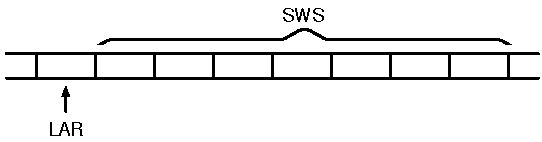
\includegraphics[bb=0bp 0bp 95mm 23mm,clip]{transmission/sliding_window_sender}

\caption{\label{fig:sliding_window_sender}Sliding-Window des Senders}

\end{figure}



\minisec{Empf�nger}

Der Empf�nger verwaltet drei Variablen:
\begin{itemize}
\item Die maximale Anzahl der Nachrichten, die der Empf�nger annimmt ohne
eine Best�tigung f�r diese gesendet zu haben, wird als Gr��e des Empfangsfensters
(engl. receive window size, RWS) bezeichnet.
\item Die Sequenznummer der zuletzt akzeptierten Nachricht (engl. last ack
sent, LAS). D.h. das ist die gr��te Sequenznummer, f�r die eine Best�tigung
geschickt wurde.
\item Die kleinste Sequenznummer, die empfangen wurde und f�r die noch keine
Best�tigung gesendet wurde (engl. first message not acknowledged,
FMN).
\end{itemize}
Die Abbildung \vref{fig:sliding_window_receiver} illustriert dies:

%
\begin{figure}[h]
\centering

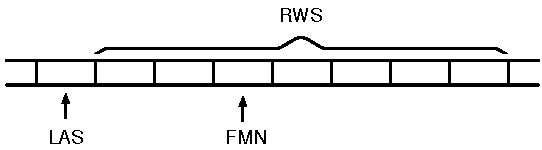
\includegraphics[bb=0bp 0bp 93mm 27mm,clip]{transmission/sliding_window_receiver}

\caption{\label{fig:sliding_window_receiver}Sliding-Window des Empf�ngers}

\end{figure}



\minisec{Algorithmus}

Der Sender schickt eine Nachricht mit der Sequenznummer SEQ ab, wenn
die Bedingung SEQ $\leq$ LAR + SWS eingehalten ist. Das sagt aus,
dass der Sender nicht mehr Nachrichten im voraus absendet als er Best�tigungen
erhalten hat. Der Sender verh�lt sich folgenderma�en:
\begin{enumerate}
\item F�r jede Nachricht, die der Sender abschickt startet er einen Timer
und legt diese Nachricht in einem Zwischenspeicher ab. Wird f�r diese
Nachricht eine Best�tigung empfangen, dann wird der Timer gestoppt.
Kommt es zu einem Zeitablauf, dann wird die Nachricht, die zu diesem
Timer geh�rt nochmals abgesendet.
\item Erh�lt der Sender eine Best�tigungsnachricht f�r die Sequenznummer
SEQ, dann setzt der Sender LAR auf SEQ (wenn SEQ gr��er als LAR).
\end{enumerate}
Der Empf�nger verh�lt sich folgenderma�en:
\begin{enumerate}
\item Erh�lt der Empf�nger eine Nachricht mit der Sequenznummer SEQ und
befindet sich diese innerhalb des Empfangsfensters, d.h. LAS $<$
SEQ $\leq$ LAS $+$ RWS, dann wird diese Nachricht akzeptiert und
zwischengespeichert, wenn eine Nachricht mit dieser SEQ noch nicht
empfangen wurde. Anderenfalls wird diese Nachricht verworfen.
\item Ist die Sequenznummer der gerade zwischengespeicherten Nachricht kleiner
als FMN, dann wird FMN zu SEQ gesetzt.
\item Ist die Bedingung FMN = LAS + 1 erf�llt, dann wird die gr��te Sequenznummer
NMA (next message to acknowledge) der empfangenen Nachrichten innerhalb
des Sliding-Window gesucht, sodass sich keine nicht empfangenen Nachrichten
zwischen NMA und FMN befinden. Es wird LAS auf NMA gesetzt und es
wird eine Best�tigungsnachricht mit NMA an den Sender gesendet. Damit
best�tigt der Empf�nger alle Nachrichten inkl. derjenigen mit der
Sequenznummer NMA. Danach wird noch FMN neu gesetzt.
\end{enumerate}

\minisec{Varianten}

Es gibt Varianten zu dem gerade beschriebenen Algorithmus:
\begin{itemize}
\item Es besteht die M�glichkeit jede empfangene Nachricht, die sich innerhalb
des Empfangsfensters befindet sofort zu best�tigen. Diese M�glichkeit
nennt man \emph{selektives} Best�tigen im Gegensatz zur gerade beschriebenen
Methode der \emph{kumulativen} Best�tigung. 
\item Im Gegensatz zu den positiven Best�tigungen kann der Empf�nger auch
negative Best�tigungen (engl. negative acknowledgments, NAK) senden,
die anzeigen, dass eine Nachricht nicht erhalten wurde.
\end{itemize}
Beiden Varianten ist gemein, dass sie die Komplexit�t der Software
vergr��ern und in gewissen Ma�e auch zu einem erh�hten Nachrichtenverkehr
f�hren. Allerdings kann der Sender schneller auf Fehler reagieren
und unter Umst�nden den verf�gbaren �bertragungskanal besser ausnutzen.


\minisec{Endliche Sequenznummern}

Nicht betrachtet wurde bei dem beschriebenen Algorithmus allerdings,
dass die Sequenznummern eine maximale Gr��e haben, die durch die Implementierung
festgelegt ist. D.h. die Sequenznummern k�nnen nicht unendlich wachsen:
sie sind endlich.

Betrachten wir zuerst den Stop-And-Go-Algorithmus mit einer 1 Bit
langen Sequenznummer. Damit gibt es 2 verschiedene Sequenznummern,
aber nur eine Nachricht darf ausst�ndig sein.

Vergr��ert man den Speicherplatz f�r die Sequenznummern auf 3 Bit,
ergibt sich ein Bereich f�r die Sequenznummern von 0 bis 7 (= SEQ$_{\text{max}}$).
Nehmen wir an, dass SWS = RWS = 7 ist und der Sender Nachrichten mit
den Sequenznummern 0 bis 6 sendet. Der Empf�nger empf�ngt diese und
sendet ACKs, die jedoch verloren gehen. D.h. aus der Sicht des Empf�ngers
sieht es so aus, dass als n�chstes die Nachricht mit der Sequenznummer
7 kommen muss und danach wieder Sequenznummern mit 0 beginnend. Beim
Sender laufen jedoch die Timer ab, sodass dieser die alten Nachrichten
mit den Sequenznummern 0 bis 6 nochmals sendet, die vom Empf�nger
jedoch als neue Nachrichten interpretiert werden w�rden.

Die Anzahl der m�glichen Sequenznummern muss gr��er sein als die der
maximalen Anzahl der ausstehenden Frames. Es muss gelten, dass: SWS
$+$ RWS $<$ SEQ$_{\text{max}}$ $+$ 1. Bei SWS = RWS folgt damit,
dass SWS $<$ (SEQ$_{\text{max}}$ $+$ 1) / 2 sein muss. D.h. analog
zum Stop-And-Go Algorithmus, der jeweils zwischen den Sequenznummern
0 und 1 wechselt, wird hier -- allerdings kontinuierlich -- zwischen
den beiden H�lften der Sequenznummern hin- und herbewegt.



\chapter{Netzarchitektur\label{sec:network_architecture}}

Der vorhergehende Abschnitt hat die Kommunikation zwischen zwei Kommunikationspartnern
behandelt. Ein Netz besteht im allgemeinen jedoch aus mehreren Kommunikationspartnern,
die miteinander verbunden sind und miteinander kommunizieren k�nnen.
Damit wird aus einer Punkt-zu-Punkt Verbindung ein Datennetz.

Ein Datennetz (engl. data network) �bertr�gt digitale Signale zwischen
Paaren oder Gruppen von Kommunikationspartnern. Dabei k�nnen Kommunikationsbeziehungen
wahlfrei zwischen beliebigen Kommunikationspartnern hergestellt werden.

Das Modell der Daten�bertragung, wie es im Abschnitt \ref{sec:communication_model}
besprochen wurde, wird zu einem Datennetz:

%
\begin{figure}[H]
\centering

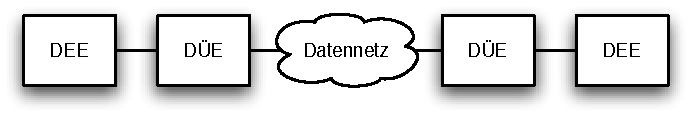
\includegraphics[bb=0bp 0bp 126mm 18mm,clip]{architecture/data_network}

\caption{Datennetz}

\end{figure}


Eine Punkt-zu-Punkt Verbindung wird von nun an als eine Spezialform
eines Datennetzes verstanden. Handelt es sich bei den DEEs um autonome
Rechner oder rechnerartige Ger�te (wie z.B. Drucker, Speichersysteme,...)
dann sprechen wir von nun an von einem Rechnernetz (engl. computer
network). Datennetze, Rechnernetze oder eben nur Netze werden, wie
im vorhergehenden Diagramm, mit einer ,,Wolke'' als Symbol gekennzeichnet.
Die Kommunikationsteilnehmer in einem Rechnernetz werden als Host
bezeichnet.

Solch ein Netz kann entweder direkt mehrere Netzteilnehmer miteinander
verbinden oder durch einen Zusammenschluss von zwei oder mehreren
Netzen entstehen:

%
\begin{figure}[H]
\centering

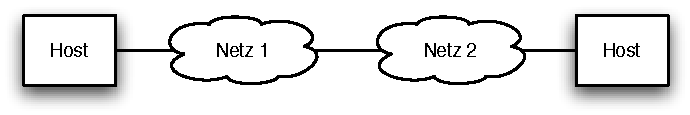
\includegraphics[bb=0bp 0bp 126mm 19mm,clip]{architecture/composed_network}

\caption{Verbundene Rechnernetze}

\end{figure}


In der vorhergehenden Abbildung wurden zum Zwecke der �bersichtlichkeit
vorerst die Netzger�te au�er Acht gelassen, die man f�r den Zusammenschluss
mehrerer Teilnetze zu einem Gesamtnetz ben�tigt. In Abschnitt \vref{sec:coupling_devices}
werden diese erl�utert. Fasst man zwei oder beliebig viele Netze zu
einem Netz zusammen, dann bezeichnet man die einzelnen Netze des entstehenden
Gesamtnetzes als Teilnetze eben dieses ganzen Netzes.

In diesem Kapitel wird im folgenden der prinzipielle Aufbau und die
Funktionsweise eines Netzes erkl�rt. 


\section{Struktur und Komponenten eines Netzes}

Ein Netz besteht aus einem oder mehreren Netzsegmenten. Mehrere Netzsegmente
sind durch Kopplungsger�te (siehe Abschnitt \ref{sec:coupling_devices})
miteinander verbunden. Netzsegmente sind daher eine Strukturierung
f�r Rechnernetze auf der phyischen Ebene.

Die logische Struktur eines Netzwerkes ist durch die Netztopologie
vorgegeben.


\subsection{Netztopologie}

Wir definieren, dass es sich bei einem Netz (engl. network) um eine
Menge von Knoten (engl. node) handelt. Je zwei Knoten werden durch
eine Teilstrecke oder Verbindung (engl. link) miteinander verbunden.
Eine Art von Knoten sind die Hosts, eine andere Art sind die Kopplungselemente,
die lediglich Netzsegmente miteinander verbinden. Jetzt betrachten
wir, in welcher Art diese Knoten miteinander zu einem Netz verbunden
werden k�nnen. Eine bestimmte Struktur des Verbindens bezeichnet man
als Topologie. Allerdings sollte beachtet werden, dass die physikalische
von der logischen Topologie abweichen kann ($\rightarrow$ Abstraktion).


\subsubsection{Vermaschtes Netz}

Das vermaschte Netz ist eine logische Weiterf�hrung der Punkt-zu-Punkt
Verbindung indem bestimmte (beliebige) Hosts direkt miteinander verbunden
werden. Ein Beispiel f�r ein solches vermaschtes Netz ist in Abbildung
\vref{fig:mashed_net} zu sehen.

%
\begin{figure}[h]
\centering

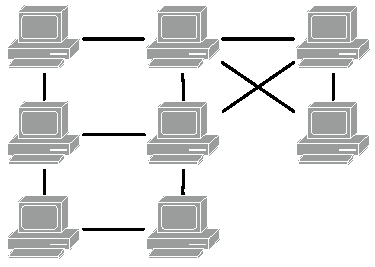
\includegraphics[bb=0bp 0bp 65mm 45mm,clip]{architecture/network_mash}

\caption{\label{fig:mashed_net}Vermaschtes Netz}

\end{figure}


Wollen nur die Hosts miteinander kommunizieren, die direkt miteinander
verbunden sind, ergibt sich eigentlich kein Unterschied zu mehreren
Punkt-zu-Punkt Verbindungen. Sollen die anderen Hosts auch miteinander
kommunizieren, dann muss ein Kommunikationspfad gefunden werden, der
diese Hosts (indirekt) miteinander verbindet und die Hosts auf diesem
Kommunikationspfad m�ssen die Nachrichten weiterreichen. F�llt ein
Host oder eine Verbindungsleitung auf einem Kommunikationspfad aus,
dann gibt es je nach Struktur des Netzes gegebenfalls alternative
Pfade, die gew�hlt werden k�nnen.

D.h. es gibt prinzipiell keine zugrundeliegende Struktur, die Verbindungen
werden nach gewissen Gesichtspunkten wie z.B. Leistung oder Ausfallsicherheit
gew�hlt.

Als Vorteile dieser Struktur k�nnen die Ausfallsicherheit und die
Leistung hervorgehoben werden, als Nachteile fallen die hohen Verkabelungskosten,
Wartungskosten und ein vergleichsweises kompliziertes Finden der Kommunikationspfade
an.


\subsubsection{Sternnetz}

Will man ein Netz einfach strukturieren, dann bietet sich eine Sternstruktur
an. Dieses war entwicklungsgeschichtlich die erste Struktur. Es wird
ein Knoten ausgezeichnet, der (haupts�chlich) eine Vermittlungsfunktion
�bernimmt und zu jedem Host im Netzwerk eine Verbindungsleitung f�hrt.
Dieser Knoten wird allgemein als Vermittlungsknoten bezeichnet (siehe
Abbildung \vref{fig:star_net}).

%
\begin{figure}[h]
\centering

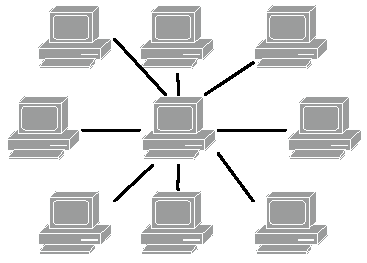
\includegraphics[bb=0bp 0bp 62mm 45mm,clip]{architecture/network_star}

\caption{\label{fig:star_net}Sternnetz}

\end{figure}


Die Vorteile in einer derartigen Struktur liegen in der einfachen
Verkabelung, der einfachen Wartbarkeit und der leichten Erweiterbarkeit.
Ein Ausfall eines Hosts hat auf die Kommunikation der anderen Hosts
keine Auswirkung. Nachteilig wirkt sich die zentrale Funktion des
Vermittlungsknotens aus: F�llt dieser aus, dann kann keine weitere
Kommunikation im Netzwerk stattfinden. Bez�glich Leistung und Erweiterbarkeit
l�sst sich sagen, dass diese lediglich von dem Vermittlungsknoten
(und nat�rlich den �bertragungskan�len) abh�ngt. Nachteilig wirkt
sich auch aus, dass die Verkabelung sehr teuer ist.


\subsubsection{Baumnetz}

Werden Sternnetze hierarchisch miteinander verbunden, dann entsteht
ein Baumnetz (siehe Abbildung \vref{fig:tree_net}). Im englischen
Sprachgebrauch werden diese auch als ,,extended star'' bezeichnet.
Verbunden werden die einzelnen Vermittlungshosts mittels sogenannter
Uplinks.

%
\begin{figure}[h]
\centering

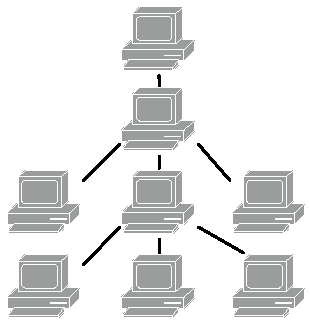
\includegraphics[bb=0bp 0bp 55mm 55mm,clip]{architecture/network_tree}

\caption{\label{fig:tree_net}Baumnetz}

\end{figure}


Die Vorteile dieser Topologie liegen in der leichten Erweiterbarkeit
und der Administrierbarkeit (Teilung der Verantwortung).


\subsubsection{Ringnetz}

Es wird jeder Host mit genau zwei anderen Hosts so verbunden, sodass
ein geschlossener Ring entsteht (siehe Abbildung \vref{fig:ring_net}).
Der eine verbundene Host wird als Vorg�nger definiert und der andere
als Nachfolger. D.h. prinzipiell ist eine Richtung in diesem Ring
vorgegeben. Der Sender sendet die Nachricht an seinen Nachfolger.
Ist die Nachricht beim Empf�nger angekommen, dann nimmt dieser die
Nachricht vom Netz, andererseits wird die Nachricht wieder an den
Nachfolger des aktuellen Knotens weitergereicht. Das wird solange
durchgef�hrt bis der Empf�nger erreicht ist.

%
\begin{figure}[h]
\centering

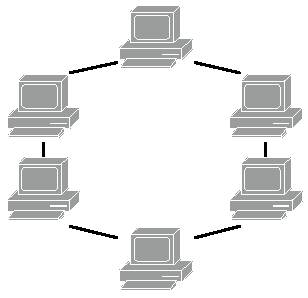
\includegraphics[bb=0bp 0bp 53mm 50mm,clip]{architecture/network_ring}

\caption{\label{fig:ring_net}Ringnetz}

\end{figure}


Die Vorteile dieser Topologie liegen darin, dass jeder Knoten eine
Signalauffrischung durchf�hrt und dadurch eine gro�e Netzausdehnungen
m�glich ist, dass kein Flaschenhals wie beim Sternnetz vorliegt und
die eigentliche Daten�bertragung sehr einfach ist, da die �bertragung
nur in einer Richtung stattfindet. An Nachteilen sind zu nennen, dass
ein Ausfall eines Knotens oder einer Verbindung den gesamten Ring
beeintr�chtigt und die Nachrichten alle Knoten am Pfad zum Empf�nger
durchlaufen m�ssen.


\subsubsection{Busnetz}

Ein Busnetz ist grunds�tzlich anders: Hier gibt es einen Bus an den
alle Knoten direkt angeschlossen sind (siehe Abbildung \vref{fig:bus_net}).
D.h. es muss einen Mechanismus geben, der den Zugriff auf das gemeinsame
Medium regelt, wenn mehrere Hosts gleichzeitig zugreifen wollen.

%
\begin{figure}[h]
\centering

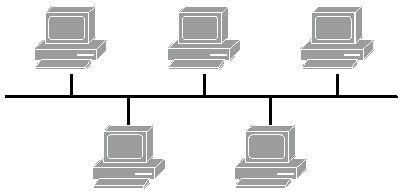
\includegraphics[bb=0bp 0bp 70mm 34mm,clip]{architecture/network_bus}

\caption{\label{fig:bus_net}Busnetz}

\end{figure}


Gro�e Vorteile liegen in der Verkabelung, der Erweiterbarkeit und
den Kosten. An Nachteilen sind zu nennen:
\begin{itemize}
\item Fehler finden ist schwieriger als bei den anderen Topologien.
\item Ein Fehler in der Verkabelung bedeutet, dass das gesamte Netzwerk
nicht mehr funktioniert.
\item Die Leistung des Netzwerks sinkt bei mehreren gleichzeitigen Zugriffen.
\item Jeder Host kann den gesamten Netzwerksverkehr lesen. Das kann unter
Umst�nden ein Sicherheitsproblem darstellen.
\end{itemize}

\subsection{Netzger�te}

Ein Rechnernetz besteht also aus Knoten und Verbindungen:
\begin{itemize}
\item Knoten sind entweder Hosts (d.h. Endger�te) oder Kopplungselemente
(z.B. ein Router), die Teilnetze miteinander verbinden.
\item Die eigentlichen Verbindungen werden mittels Kabel, Stecker und Netzzugangsger�ten
(z.B. eine Schnittstellenkarte) realisiert.
\end{itemize}
Alle diese in einem Rechnernetz konkret vorkommenden Ger�te werden
als Netzger�te bezeichnet.


\subsubsection{Zugriffsverfahren\label{sec:access_method}}

Ein Netzzugangssger�t speist die Signale in das �bertragungsmedium
ein. Da mindestens 2 Kommunikationspartner auf das �bertragungsmedium
zugreifen wollen, muss es ein Verfahren geben, das diesen Zugriff
regelt. Man unterscheidet:
\begin{description}
\item [{Reservierungsverfahren}] Bei den Reservierungsverfahren wird zu
Beginn eine Reservierung vereinbart. Die Multiplexverfahren sind solche
Verfahren.
\item [{Zuteilungsverfahren}] Der Zugriff auf das �bertragungsmedium wird
zugeteilt, d.h. der Zugriff findet geregelt statt. Diese Erteilung
des Zugriffes kann entweder zentral (z.B. mittels polling) oder dezentral
(z.B. mittels token passing) erfolgen.
\item [{Wettbewerbsverfahren}] Diese funktionieren im Prinzip so, dass
jeder Sender versucht auf den Kanal zu senden, wenn dieser frei ist.
Der Sender, der einen freien Kanal vorfindet, beginnt zu senden. Vertreter
sind CSMA/CD (carrier sense multiple access/collision detection) oder
CSMA/CA (carrier sense multiple access/collision avoidance).
\end{description}
Unter dem Begriff \emph{Kollisionsdom�ne} (engl. collision domain)
wird in einem Computernetz ein Bereich bezeichnet, in dem Kollisionen
auftreten k�nnen. Sie entstehen, wenn zwei Stationen gleichzeitig
versuchen, auf einem einzigen physikalischen Medium (Segment) etwas
zu senden. Die Spannungsimpulse werden im Kabel vermischt und die
Signale somit zerst�rt.

Eine \emph{Broadcastdom�ne} ist ein logischer Verbund von Computern
in einem lokalen Netzwerk, der sich dadurch auszeichnet, dass ein
Broadcast alle Dom�nenteilnehmer erreicht.


\subsubsection{Netzzugangsger�te}

Im Prinzip kann man zwei Arten von Netzzugangsger�ten unterscheiden,
je nachdem, ob es sich um einen Breitbandzugang oder einen Basisbandzugang
handelt.
\begin{description}
\item [{Modem}] Ein Modem moduliert und demoduliert ein analoges Signal,
um digitale Daten �bertragen zu k�nnen. D.h. die digitalen Daten werden
z.B. auf ein hochfrequentes Tr�gersignal aufmoduliert. Urspr�nglich
wurden Modems haupts�chlich verwendet, um Daten �ber normale Telefonleitungen
�bertragen zu k�nnen. Danach wurde ISDN eingef�hrt und mittels ISDN
Modems (PCM, pulse code modulation) auf das ISDN Netzwerk zugegriffen.
Heute gibt es auch Kabelmodems bzw. ADSL Modems.


Der Zugriff von einem Host zu einem Modem kann �ber eine der verf�gbaren
Schnittstellen wie z.B. RS-232 oder USB erfolgen.

\item [{Schnittstellenkarte}] Eine Schnittstellenkarte (engl. network card
oder network interface card, kurz NIC) oder auch Netzwerkadapter (engl.
network adapter) genannt, ist im Sinne der Daten�bertragung eine Daten�bertragungseinrichtung,
die es dem Computer erlaubt �ber das Netz zu kommunizieren.


F�r jede NIC gibt es eine MAC Adresse und eine eigene Netzwerkadresse.

\end{description}

\subsubsection{Kopplungselemente\label{sec:coupling_devices}}

Netze k�nnen auf der physikalischen Ebene mittels Kopplungselementen
verbunden werden. Die mit solchen Kopplungselementen verbundenen Teilnetze
werden als Netzsegmente bezeichnet. Der Anschluss eines Kopplungselementes
f�r ein Netzwerksegment wird auch Port genannt.
\begin{description}
\item [{Repeater}] Ein Repeater (dt. Wiederholer) hat die Aufgabe Signale
zu empfangen, diese zu regenerieren (verst�rken, verbessern) und danach
weiterzusenden. Repeater verbinden zwei (oder mehrere) Netzwerksegmente
gleichen Typs zu einem gr��eren Netzsegment.


Die prim�re Aufgabe von Repeatern ist, die physikalische Ausdehnung
des Netzwerkes zu erh�hen. Repeater arbeiten auf der ISO/OSI Schicht
1.

Ein Netzsegment, das auf diese Weise mittels Repeater aus mehreren
Netzsegmenten entstanden ist, verh�lt sich als Kollisionsdom�ne.

\item [{Hub}] Ein Hub (dt. zentraler Knoten, Mittelpunkt, Drehscheibe)
ist lediglich ein Repeater, der mehrere Netzsegmente miteinander verbindet
(d.h. diese haben mehrere Ports). Hubs werden auch Multiport-Repeater
genannt. Dieser Begriff wird h�ufig im Ethernet verwendet.
\item [{Bridge}] Eine Bridge (dt. Br�cke) verbindet zwei Netzwerkssegmente
auf der ISO/OSI Schicht 2 zu einem gr��eren Netz. Anders gesehen teilt
eine Br�cke ein Netz in zwei Netzsegmente. Haben die Netzsegmente
unterschiedliche Zugriffsverfahren, werden diese von der Bridge angepasst.


Eine Bridge gibt nur Rahmen weiter, deren MAC Adresse in dem entsprechenden
Netzsegment liegt. Bridges trennen Netzsegmente daher sowohl physisch
als auch logisch. Damit endet eine Kollisionsdom�ne an einer Bridge.

\item [{Switch}] Ein Switch (dt. Schalter) verbindet mehrere Netzwerksegmente
auf der ISO/OSI Schicht 2. Ein Switch arbeitet prinzipiell in einem
von zwei Modi: Ein \emph{Store-and-Forward} Switch nimmt immer einen
ganzen Frame auf, speichert diesen zwischen, analysiert diesen und
gibt diesen am richtigen Zielport wieder aus. Ein \emph{Cut-Through}
Switch nutzt die Tatsache, dass sich in einem Ethernet Frame die Zieladresse
am Anfang befindet und leitet den Frame zum Zielport weiter, nachdem
der lediglich der Frame bis inkl. der Zieladresse gelesen wurde. Der
Vorteil eines Store-and-Forward Switch ist, dass dieser nur g�ltige
Frames weiterreicht, w�hrend ein Cut-Through Switch eine h�here Performance
aufweist daf�r aber auch fehlerhafte Frames weiterleitet.


Die Methode wie ein Switch den richtigen Zielport f�r einen Frame
kennen lernt, wird als Backward-Learning bezeichnet: Jedes Mal, wenn
ein Switch einen Frame an einem Port erh�lt, merkt sich der Switch
die Quell-MAC (siehe Abschnitt \vref{sec:addresses}) gemeinsam mit
dem Port an dem der Frame empfangen wurde. Kennt der Switch die die
Ziel-MAC nicht, wird der Frame an allen anderen Ports weitergeleitet.
Diesen Vorgang nennt man Fluten (port flooding). Auf diese Weise erreicht
der Frame sein Ziel. Sendet der Empf�nger einen Frame zur�ck an den
urspr�nglichen Sender, dann merken sich die Switches auch dessen MAC,
wodurch bei wiederholten Senden zwischen diesen beiden Hosts kein
Fluten mehr notwendig ist.

\item [{Router}] Ein Router (dt. Vermittler) verbindet mehrere Netze miteinander
und hat die Aufgabe eine empfangene Nachricht an das richtige Netz
weiterzuleiten, sodass der eigentliche Empf�nger letztendlich die
Nachricht erh�lt. Router m�ssen dazu den Netzaufbau in gewisser Weise
kennen.


An einem Router endet sowohl eine Kollisionsdom�ne als auch eine Broadcastdom�ne.

Ein Router arbeitet auf der ISO/OSI Schicht 3.

\item [{Gateway}] Das Gateway verbindet ebenfalls mehrere Netze miteinander,
unterscheidet sich von einem Router jedoch dadurch, dass ein Gateway
Netze mit verschiedenen Anwendungsprotokollen verbindet. D.h. ein
Gateway �bersetzt ein Anwendungsprotokoll in ein anderes Anwendungsprotokoll.
Ein einfaches Beispiel f�r ein Gateway ist ein http Proxy.


Gateways arbeiten auf der ISO/OSI Schicht 7.

\end{description}
Die folgende Abbildung gibt einen �berblick �ber die verschiedenen
Arten der Kopplungssysteme im Zusammenhang mit dem OSI Modell.

%
\begin{figure}[h]
\centering

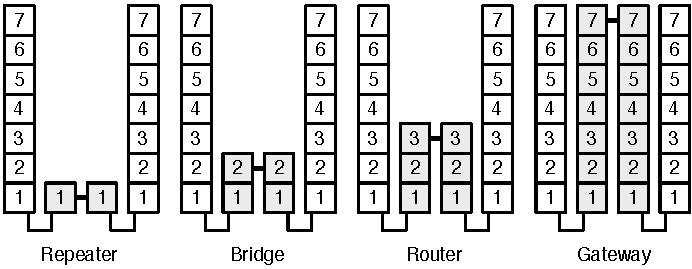
\includegraphics[bb=0bp 0bp 12cm 5cm,clip]{architecture/coupling_devices}

\caption{�bersicht �ber die Kopplungssysteme}

\end{figure}



\subsection{Netzstrukturen}

Netze k�nnen -- unabh�ngig von ihren -- Topologien beliebig miteinander
verbunden werden.


\subsubsection{Netzhierarchie}

Gr��ere Netze werden hierarchisch in Schichten aufgebaut.
\begin{itemize}
\item Auf der untersten Ebene befinden sich die \emph{lokalen Netzwerke},
die Netzger�te innerhalb einer begrenzten Umgebung miteinander verbinden.
Solche Netze k�nnen nat�rlich auch wieder miteinander verbunden sein.
Ein typischer Vertreter einer solchen Netztechnologie ist Ethernet.
\item Um einen Zugang zu weiter entfernten Hosts zu bekommen, werden die
lokalen Netze mittels \emph{Zugangsnetze} (engl. access networks)
an ein �bergeordnetes Netzwerk verbunden. Beispielsweise kann ein
Einzelcomputer mittels ADSL als Zugangsnetz an das Netz des Providers
angeschlossen werden. Beispiele f�r weitere Technologien sind ISDN,
DSL Varianten oder Richtfunkstrecken.\\
Im Bereich der Zugangsnetze wird oft PPP (Point-to-Point Protocol)
verwendet, das eine Punkt-zu-Punkt Verbindung herstellt und verschiedenste
Netzprotokolle (wie z.B. IP, IPX, AppleTalk) transportieren kann.
F�r den Betrieb von PPP �ber Ethernet gibt es die modifizierte Variante
PPPoE (Point-to-Point over Ethernet). Auch das PPTP (siehe Abschnitt
\vref{sec:VPN}) wird oft f�r Zugangsnetze verwendet.
\item �ber das Zugangsnetz werden die Hosts an ein \emph{Verteilungsnetz}
(engl. distribution network) angeschlossen. Dabei handelt es sich
z.B. um ein Firmennetz, das mittels eines Backbones mehrere Firmenstandorte
verbindet oder um das Netz eines Providers. Das Verteilungsnetz grenzt
Zugangsnetze von einem Kern-Netzwerk ab (z.B. dem globalen Internet).
In einem Verteilungsnetz werden auch noch Funktionen wie Adressumsetzung
(engl. network address translation, NAT), Sicherheits�berpr�fungen
oder VLAN Routing implementiert. Als Technologien kommen z.B. FDDI,
ATM oder auch Gigabit-Ethernet zum Einsatz.
\item Ein Kernnetz (engl. core network) dient der weltweiten Vernetzung.
Als Technologien werden Standleitungen, ATM und auch Frame Relay eingesetzt.
\end{itemize}
Ein Beispiel f�r eine derartige Netzhierarchie ist in der Abbildung
\vref{fig:net_hierarchy} zu finden.

%
\begin{figure}[h]
\centering

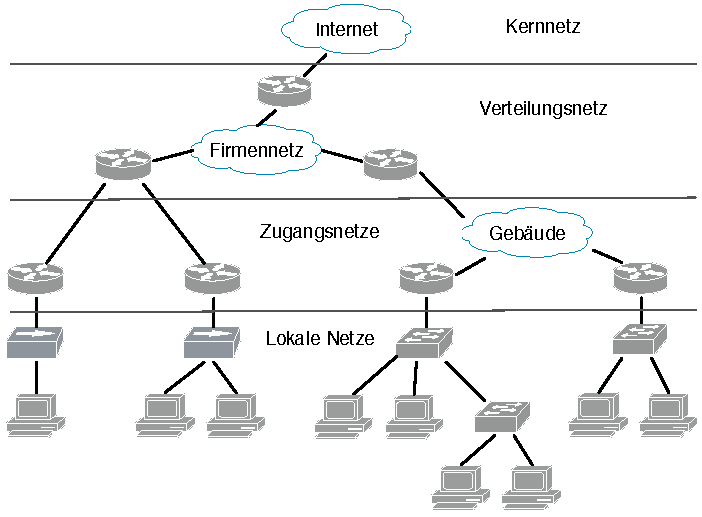
\includegraphics[bb=0bp 0bp 120mm 88mm,clip]{architecture/network_hierarchy}

\caption{\label{fig:net_hierarchy}Beispiel einer Netzhierarchie}

\end{figure}



\subsubsection{Strukturierte Verkabelung\label{sec:structured_cabeling}}

Eine konkrete Auspr�gung einer Netzhierarchie ist die Verkabelung
eines Standortes. Die europ�ische Norm EN 50173-1 ist unter dem Begriff
\emph{strukturierte Verkabelung} bekannt. Meist wird hierf�r als Topologie
eine Baumtopologie verwendet.

Dazu wird die Verkabelung in Prim�rbereich, Sekund�rbereich und Terti�rbereich
eingeteilt.

Der Prim�rbereich deckt die Verbindung der einzelnen Geb�ude untereinander
ab. Dazu gibt es je Geb�ude einen Hauptverteiler, die direkt mit den
anderen Geb�uden verbunden sind. Der Sekund�rbereich �bernimmt die
(vertikale) Stockwerksverkabelung und verbindet hiermit die einzelnen
Etagenverteiler mittels Stichleitungen mit dem Hauptverteiler. Der
Terti�rbereich stellt die horizontale Stockwerksverkabelung dar und
verbindet die einzelnen Arbeitsstationen mittels Stichleitungen mit
dem Etagenverteiler.

Um flexibel zu sein, werden die Verteiler mittels Patchfelder (engl.
patch panel) realisiert. Hierunter versteht man ein Schaltfeld, das
alle Leitungen an Buchsen f�hrt. Die Verbindungen werden mittels Patchkabel
hergestellt.


\subsubsection{VLAN}

Ein VLAN (engl. virtual local area network) ist ein virtuelles lokales
Netzwerk innerhalb eines LAN. Mit VLANs k�nnen mehrere logische Netze
innerhalb eines physisches LAN betrieben werden. Sie dienen also dazu
eine weitere Struktur in ein physisches Netz zu legen.

VLANs will man im Prinzip aus folgenden Gr�nden einrichten:
\begin{itemize}
\item Flexibilit�t beim Aufbau der Netze, da die logischen Netze unabh�ngig
zum physischen Aufbau des LAN ist.
\item Einsparung von Routern und damit eine vereinfachte Verwaltung sowie
eine Verringerung der Latenz.
\item Verringerung der Broadcast-Last, denn jedes VLAN bildet eine eigene
Broadcast-Dom�ne.
\item Steigerung der Sicherheit, denn es kann nicht auf die Daten eines
anderen Netzes zugegriffen werden.
\end{itemize}
Die standardisierte Grundlage f�r den Betrieb von VLANs liegt in IEEE
802.1Q begr�ndet (es gibt jedoch auch herstellerspezifische Implementierungen).
Die Implementierung von VLANs basiert im Prinzip darauf, dass dem
Ethernet-Frame 4 Bytes an zus�tzlicher Headerinformation hinzugef�gt
wird. Von diesen 4 Bytes werden 12 Bit zur Aufnahme einer VLAN ID
verwendet. Daraus resultiert eine maximale Anzahl von 4094 VLANs,
da die IDs mit lauter Nullen bzw. lauter Einsen reserviert sind und
nicht zur Verf�gung stehen.


\subsubsection{VPN\label{sec:VPN}}

Ein VPN (engl. virtual private network) ist ein Netz von zwei oder
mehreren Rechnern, die �ber Tunnels (�bertragen der Daten eines Protokolls
eingebettet in ein anderes Protokolls) verbunden sind. Ein VPN wird
(meist) �ffentlich verwendet und ist in der Regel durch kryptographische
Verfahren gesichert. VPNs transportieren im Normalfall ISO/OSI Schicht
2 Frames oder Schicht 3 Pakete.

Als Anwendung wird ein VPN oft verwendet, um Au�enstellen oder externen
Mitarbeitern den Zugriff auf das Unternehmensnetzwerk zu erm�glichen.
Wichtig ist, dass der Client ebenfalls richtig konfiguriert ist, sodass
die gesamte Kommunikation des Clients nach dem �ffnen des VPN-Zugangs
�ber den VPN-Pfad l�uft!

Um ein vollst�ndiges VPN zu bilden m�ssen drei Komponenten kombiniert
werden: Tunnels, Verschl�sselung und Authentifizierung.

Einige ,,wichtige'' Protokolle mit, denen ein VPN aufgebaut werden
kann, sind:
\begin{labeling}{00.00.0000}
\item [{PPTP}] (point-to-point tunneling protocol) erm�glicht das Tunneling
von PPP durch ein IP Netzwerk. Es wird oft als Zugangsnetz f�r die
Anbindung von privaten Nutzern an die Internet Service Provider verwendet,
obwohl es relativ unsicher ist. Eine Verschl�sselung ist im Prinzip
in diesem Standard vorgesehen und muss durch h�here Protokolle realisiert
werden (abgesehen von der Microsoft-spezifischen Erweiterung MPPE,
die PPP Pakete verschl�sselt). Der ,,einzige'' Vorteil von PPTP
ist, dass es in Windows vorinstallliert ist.
\item [{L2TP}] (layer 2 tunneling protocol) ist in etwa von der Funktionalit�t
dem PPTP �hnlich und ebenfalls relativ unsicher. Erst die Kombination
mit IPSec erm�glicht auch eine Verschl�sselung.
\item [{IPSec}] IPSec (siehe Abschnitt \vref{sec:IPSec}) ist eine Gruppe
von Protokollen zur Verschl�sselung. Es befindet sich auf der Schicht
3 und kann Protokolle ab (inklusive) Schicht 3 transportieren und
sichern. Es wurde urspr�nglich f�r IPv4 entwickelt und als Kernkomponente
bzgl. Sicherheit in IPv6 eingegliedert. Es gilt als ausreichend sicher,
wenn es richtig konfiguriert wird. Jedes Betriebssystem ben�tigt seine
eigene Implementierung im TCP/IP Stack.
\item [{TLS/SSL}] Mittels TLS/SSL (siehe Abschnitt \vref{sec:TLS}) kann
ebenfalls ein VPN aufgebaut werden (siehe das Produkt OpenVPN im Abschnitt
\vref{sec:OpenVPN}).


Mit TLS kann auch ein einfacher Tunnel aufgebaut werden. Die Vor-
und Nachteile sind analog zu der Technik mit SSH wie im n�chsten Punkt
beschrieben. Als Produkt gibt es z.B. Stunnel (siehe Abschnitt \vref{sec:Stunnel}),
das es einfach erlaubt verschiedene Protokolle �ber TLS zu tunneln.

\item [{SSH}] Auch mittels SSH (secure shell, siehe Abschnitt \vref{sec:SSH_protocol})
kann ein Tunnel aufgebaut werden. Allerdings ist SSH nicht f�r eine
permanente LAN-zu-LAN und Client-zu-LAN Verbindungen geeignet, da
mittels SSH nur Socket-Tunnels m�glich sind. Allerdings entsteht gerade
dadurch ein Vorteil, da die Tunnels je Applikation spezifisch sind.
Ein kompromittierter Tunneleingang einer SSH Verbindung betrifft nur
die Applikation bzw. den Port am Tunnelende und nicht das gesamte
Netz, das mit dem Tunnelende verbunden ist!
\end{labeling}

\subsection{Netzsoftware}

In einem verteilten System kann man die Software prinzipiell in drei
Klassen einteilen:
\begin{itemize}
\item Die verteilte Anwendung an sich. D.h. es handelt sich um die Software,
die oberhalb der Schicht 7 angesiedelt ist.
\item Meistens ben�tigt die Anwendung noch unterst�tzende Software, die
bestimmte Dienste zur Kommunikation, Synchronisierung, Transaktionsverwaltung,\ldots{}
zur Verf�gung stellt. Diese Software ist meistens zwischen der Schicht
7 und der eigentlichen Anwendung (also in der Mitte) angesiedelt.
Diese Software wird aus diesem Grund auch Middleware genannt.
\item Unbedingt erforderlich ist die eigentliche Netzsoftware, die die gesamte
Kommunikation erm�glicht. Wie schon erl�utert, handelt es sich meistens
um eine Implementierung eines Protokollstacks (z.B. ISO/OSI oder am
h�ufigsten TCP/IP).
\end{itemize}

\section{Vermittlung und Weiterleitung}

In diesem Abschnitt wird zuerst die Adressierung der Knoten besprochen,
dann die Prinzipien der Paketvermittlung behandelt und danach der
grundlegende Ablauf des Weiterleitens angef�hrt als auch die Suche
eines Weges zwischen je zwei Knoten behandelt. Alle diese Themen sind
der Schicht 3 des OSI Modells zuzuordnen.


\subsection{Adressierung\label{sec:addresses}}


\minisec{Adressen}

Jeder Knoten ben�tigt im Netz bzw. im Netzsegment eine eindeutige
Adresse. Solch eine Adresse ist in der Regel ein nummerischer Wert.
Adressen sind abh�ngig von der Schicht in der sie verwendet werden:
\begin{itemize}
\item In der Schicht 2 werden diese Adressen als MAC Adressen bezeichnet
\item Im Internet sind die Adressen in der Schicht 3 die sogenannten IP
Adressen.
\item In der Schicht 4 wird im Internet als Adresse die Kombination aus
IP Adresse, Port und Protokoll verwendet.
\end{itemize}
Eine Adresse in der Schicht 2 muss nicht unbedingt global eindeutig
sein. Es reicht, dass so eine Adresse nur innerhalb eines Teilnetzes
eindeutig ist. So eine Adresse nennt man auch lokale Adresse im Gegensatz
zu einer globalen Adresse, die im gesamten Netz eindeutig sein muss
(z.B. eine IP Adresse).

Teilweise muss beim �bergang zwischen den Schichten auch zwischen
den Adressen gewandelt werden, z.B. muss eine IP Adresse in eine MAC
Adresse aufgel�st werden. Dieser Vorgang wird Adressaufl�sung (engl.
address resolution) genannt.

Es k�nnen verschiedene Typen von Adressen unterschieden werden:
\begin{itemize}
\item Die Individualadresse identifiziert genau einen Knoten.
\item Eine Gruppenadresse identifiziert eine Gruppe von Knoten. Diese Knoten
k�nnen sich auch in verschiedenen Netzen befinden. Es handelt sich
um eine Multicast-Adresse.
\item Eine Broadcast-Adresse ist eine spezielle Adresse, die alle Knoten
in einem Netz identifiziert.
\end{itemize}
Adressen k�nnen entweder flach sein oder hierarchisch aufgebaut sein.
Bei einer flachen Adresse gibt es keinen Zusammenhang zwischen der
Adresse und der geographischen Lage des Knotens, dem diese Adresse
zugewiesen wird. Bei hierarchischen Adressen gibt es solch einen Zusammenhang.
Beispiel eines flachen Adressraumes sind die MAC Adressen der Ethernet-Technologie
und ein Beispiel hierarchischer Adressen sind die IP-Adressen.

In weiterer Folge betrachten wir die hierarchisch aufgebauten IP Adressen.
Jede IP Adresse besteht aus zwei Teilen: einem Netzanteil und einem
Hostanteil. Der Netzanteil gibt das Teilnetz an, in dem der Host zu
finden ist und der Hostanteil ist die Adresse des Host in diesem Teilnetz.
Die Teilnetzangabe ist einer geographischen Lage zugeordnet.


\minisec{Namen}

Im Gegensatz zu den Adressen sind die Namen symbolische Werte, die
an der Stelle der (nummerischen) Adressen verwendet werden. Da f�r
die eindeutige Adressierung jedoch die Adresse notwendig ist, werden
Namensdienste bzw. Verzeichnisdienste ben�tigt, die einen Namen auf
eine Adresse abbilden.

Der Grund in der Verwendung von Namen liegt entweder in der leichteren
Merkbarkeit oder in der gew�nschten Einf�hrung einer Indirektion.
Eine Indirektion kann z.B. notwendig sein, um Ortstransparenz zu erreichen.
Damit ist es m�glich einen Server eines Dienstes in ein anderes Netz
zu verlegen, d.h. die Adresse zu �ndern.


\minisec{Label}

Bei verbindungsorientierten Netzen reicht es, wenn die Kopplungselemente
f�r jede ihrer Verbindungen zu den n�chsten Knoten jeweils einen eindeutigen
lokalen Bezeichner vergeben. Solch ein Bezeichner wird Label genannt.
Eine genauere Beschreibung ist in Abschnitt \vref{sec:connection-oriented_forwarding}
zu finden.


\subsection{Paketvermittlung \label{sec:packet_switching}}

In diesem und den weiteren Abschnitten wird von nun an nur mehr die
Paketvermittlung (engl. packet switching) behandelt. Dazu werden die
Nutzdaten in Pakete (engl. packet) aufgeteilt und zusammen mit anderen
Paketen im asynchronen Zeitmultiplexverfahren �ber Teilstrecken �bertragen.
Teilstrecken sind �ber Knoten miteinander verbunden, die als Router
bezeichnet werden.

Der grundlegende Ablauf in einem Router sieht so aus, dass ankommende
Pakete zwischengespeichert werden (store), dann der n�chste Router
ermittelt wird und das Paket an die richtige Ausgabeschnittstelle
weitergeleitet (engl. forwarding) wird.

Da das Speichern des Paketes, das Analysieren des Headers (z.B. Berechnen
einer Pr�fsumme) und unter Umst�nden das Ver�ndern des Headers (z.B.
siehe TTL im Abschnitt \ref{sec:ip}) relativ lange dauert, hat man
Spezialformen der Paketvermittlung geschaffen, die diese Nachteile
vermeiden. Einerseits handelt es sich um das Konzept Frame Relay (Pakete
mit variabler L�nge) und Cell Relay (Paket mit fixer L�nge).

Im Prinzip gibt es 3 M�glichkeiten: verbindungsloses Weiterleiten,
verbindungsorientiertes Weiterleiten und Source-Routing.


\subsubsection{Verbindungsloses Weiterleiten}

Das Prinzip ist, dass ein Paket gen�gend Informationen enth�lt, damit
jedes Kopplungselement wei� wie das Paket zum Ziel weiterzuleiten
ist. Daf�r ist zumindest die Netzadresse des Ziels notwendig.

Das verbindungslose Weiterleiten weist folgende Merkmale auf:
\begin{itemize}
\item Ein Knoten kann jederzeit ein Paket zu jedem beliebigen anderen Knoten
schicken.
\item Es besteht f�r den Knoten keine M�glichkeit zu eruieren, ob das Paket
am Zielknoten ankommt bzw. ob der Zielknoten �berhaupt erreichbar
ist.
\item Jede Nachricht wird unabh�ngig von den anderen Paketen gesendet. Obwohl
zwei Pakete unter Umst�nden dasselbe Ziel haben, k�nnen die Pakete
unterschiedliche Wege im Netz nehmen, nicht in der Reihenfolge des
Sendens ankommen oder auch mehrfach das Ziel erreichen.
\item Der Ausfall eines Kopplungselementes kann unter Umst�nden vom Netz
kompensiert werden, indem ein Paket einen anderen Weg zum Ziel nimmt.
\end{itemize}

\subsubsection{Verbindungsorientiertes Weiterleiten\label{sec:connection-oriented_forwarding}}

Beim verbindungsorientiertem Weiterleiten wird zuerst eine virtuelle
Verbindung aufgebaut. Es wird deshalb auch von virtueller Leitungsvermittlung
gesprochen. Virtuell deshalb, weil eben keine echte Leitungen geschalten
werden.

Im Prinzip gibt es zwei M�glichkeiten:
\begin{enumerate}
\item Das Konzept der Verbindung wird nur von den beiden Endsystemen umgesetzt.
Die zwischenliegenden Knoten wissen von Verbindungen nichts und �bertragen
die Pakete mittels verbindungslosem Weiterleiten. Dies ist so in TCP
umgesetzt (siehe Teil \ref{par:tcpip}). In diesem Sinne handelt es
sich eigentlich gar nicht um eine virtuelle Leitungsvermittlung!
\item Das Konzept der Verbindung wird von den beiden Endsystemen \emph{und}
den Zwischensystemen umgesetzt. D.h. beim Verbindungsaufbau wird ein
Weg zwischen den beiden Endsystemen gesucht und alle auf diesem Weg
befindlichen Zwischensysteme tragen sich entsprechende Informationen
in ihren Weiterleitungstabellen (siehe Abschnitt \vref{sec:forwarding})
ein. Bei den Informationen, die eingetragen werden handelt es sich
um sogenannte Labels (dt. Marken), die einen logischen Kanal zwischen
zwei Knoten identifizieren. Pro Zwischenstation gibt es zwei Eintr�ge.
Ein Eintrag umfasst den Eingangsport und ein Label und ein Eintrag
umfasst den Ausgangsport und ein Label. D.h. bei diesen Labels handelt
es sich um lokal eindeutige Bezeichner, die zwischen zwei Knoten einen
Teil der virtuellen Leitung identifiziert. Solch ein System wird z.B.
bei X.25 verwendet. Beim Verbindungsabbau werden alle Eintr�ge in
den Zwischensystemen wieder entfernt. 
\end{enumerate}
Unter \emph{Signalisierung} versteht man in diesem Zusammenhang den
Austausch der Nachrichten, die zum Aufbau, der �berwachung und dem
Abbau einer Verbindung notwendig sind. Einerseits gibt es die �ltere
\emph{In-Band-Signalisierung} (engl. in-band signalling), die f�r
diese Steuernachrichten den gleichen logischen Kanal verwendet wie
die Nutzdaten und andererseits die modernere \emph{Au�er-Band-Signalisierung}
(engl. out-of-band signalling), die f�r die Steuernachrichten einen
getrennten logischen Kanal benutzt.


\subsubsection{Source-Routing}

Beim Source-Routing wird in jeder Nachricht gespeichert, welchen Weg
diese Nachricht durch das Netz nehmen soll. Es handelt sich hierbei
nat�rlich um eine beliebig lange Information, die in den Header der
Nachricht eingesetzt werden muss. Dieses Verfahren setzt allerdings
voraus, dass der Sender gen�gend Information �ber die Netztopologie
zur Verf�gung hat, damit er diese Informationen in den Header einf�gen
kann.

Verwendet wird dieses Verfahren selten, da es nicht gut skaliert.
Eine Anwendung ist: der Empf�nger will, dass die Nachrichten einen
bestimmten Weg nehmen sollen. Auf Grund von Sicherheits�berlegungen
werden solche Pakete von Firewalls meistens blockiert.


\subsection{Weiterleitung in IP\label{sec:forwarding}}

Wir betrachten hier die Weiterleitung wie es im Prinzip in IP umgesetzt
wird. Zum Weiterleiten enth�lt jeder Router eine Weiterleitungstabelle.
Jeder Eintrag dieser Weiterleitungstabelle enth�lt einerseits eine
Netznummer und andererseits eine Adresse eines Routers, der mit dieser
Netznummer direkt oder indirekt verbunden ist. Der n�chste Schritt
in einem Weg zum Ziel wird auch als Hop bezeichnet.

Wie es zum Aufbau solch einer Weiterleitungstabelle kommt, ist die
Aufgabe des Routing (siehe Abschnitt \ref{sec:routing}).

Die prinzipielle Vorgehensweise in einem Router beim Weiterleiten
sieht folgenderma�en aus:
\begin{enumerate}
\item Paket zwischenspeichern.
\item Header kontrollieren (Struktur und Pr�fsummen).
\item Zieladresse aus Header lesen.
\item Wenn Netznummer der Zieladresse gleich mit der Netznummer eines lokalen
Netzes,

\begin{enumerate}
\item dann: Paket an diesem Interface ausliefern, das zu diesem Netz f�hrt.
\item anderenfalls: Wenn Router f�r diese Netznummer der Zieladresse in
Weiterleitungstabelle vorhanden,

\begin{enumerate}
\item dann: Paket an den zugeh�rigen Router senden.
\item anderenfalls: Paket an den Default-Router senden.
\end{enumerate}
\end{enumerate}
\end{enumerate}

\subsection{Routing\label{sec:routing}}

Das Routing ist das Suchen von Wegen von einem Knoten des Netzwerks
zu einem anderen Knoten. D.h. es ist ein Verfahren der Wegsuche und
damit etwas ganz Anderes als das Weiterleiten, das davon ausgeht,
dass ein Weg schon gefunden ist. Als Ergebnis des Routings ergibt
sich eine Weiterleitungstabelle (auch Routingtabelle genannt), die
direkt beim Weiterleiten verwendet wird. Achtung: Routing und Weiterleiten
wird oft synomym verwendet.

Wie werden nun diese Weiterleitungstabellen erstellt? Dazu wird das
Netz als ein Graph betrachtet, dessen Kanten mit den Kosten bezeichnet
werden, die dieser Verbindung zugeordnet sind. Diese Kosten geben
Aufschluss inwieweit es w�nschenswert ist, Verkehr �ber diese Verbindung
zu senden. D.h. je kleiner die Kosten sind, desto besser ist es diese
Verbindung zu verwenden. Was diese Kosten wirklich bedeuten, wie man
zu diesen Kosten kommt und inweit sich diese Kosten im Laufe der Zeit
�ndern k�nnen, werden wir nicht im Detail betrachten. Beispielsweise
k�nnte als Kosten die �bertragungsleistung (bzw. die inverse �bertragungsleistung)
des �bertragungskanals herangezogen werden. 

Wir gehen der Einfachheit halber davon aus, dass der Hin- und der
R�ckweg gleich gewichtet sind und verwenden daher nur eine ungerichtete
Kante zwischen zwei Knoten anstatt zwei gerichteten Kanten.

Das einfachste Ma� f�r die Kosten ist, einfach die Anzahl der Hops
zu z�hlen. Damit sind die Kanten auch gleich gewichtet und damit k�nnen
ungerichtete Kanten verwendet werden. Diese Art der Kosten wird auch
in den kommenden Beispielen verwendet!

F�r das eigentliche Erstellen dieser Weiterleitungstabellen gibt es
mehrere Ans�tze:
\begin{description}
\item [{Statisches~Verfahren}] Die Weiterleitungstabellen werden einmal
erstellt. Damit ist dieses Verfahren aus der Sicht der Administration
aufw�ndig und unflexibel. Problematischer sind au�erdem zeitweilige
Ausf�lle von Verbindungen, da daf�r kurzfristig �nderungen in allen
Weiterleitungstabellen notwendig w�ren, die auf dieser Basis jedoch
praktisch nicht durchgef�hrt werden k�nnen. Das statische Verfahren
wird heutzutage nur noch f�r provisorische Zwecke sowie f�r kleine
Netze angewendet, in denen sich die Topologie kaum �ndert. 
\item [{Isolierte~Verfahren}] Bei den isolierten Verfahren verwendet jeder
Knoten nur die ihm verf�gbare, lokale Information f�r die Routing-Entscheidungen.
Dazu z�hlen so einfache Verfahren wie das Fluten (engl. flooding),
das einfach ein Paket an alle Schnittstellen weiterreicht. Ein weiteres
Verfahren ist ,,Hot Potato'' (dt. hei�e Kartoffel), das ein Paket
so schnell wie m�glich weitergibt. Dazu wird das Paket an derjenigen
Schnittstelle ausgegeben, die gerade die k�rzeste Warteschlange hat.
\item [{Zentrale~Verfahren}] Es gibt eine zentrale Stelle, die die Informationen
der Weiterleitungstabellen an alle anderen Router verteilt. Diese
zentrale Stelle muss die gesamte Netzstruktur kennen und muss entsprechend
ausfallsicher sein. Unter Umst�nden kann sich diese zentrale Stelle
als Flaschenhals erweisen.
\item [{Verteilte~Verfahren}] Die verteilten Verfahren sind dadurch gekennzeichnet,
dass jeder Router seine Routing-Entscheidungen selbstst�ndig trifft.
In TCP/IP haben sich zwei grundlegende Algorithmen f�r verteilte Verfahren
etabliert: der Distanzvektor-Algorithmus und der Link-State-Algorithmus.
\end{description}
Zentrale und verteilte Verfahren werden im Gegensatz zu statischen
Verfahren als adaptive Verfahren bezeichnet, da auf �nderungen der
Netztopologie reagiert werden kann.

Als Beispiel f�r die beiden Algorithmen wird der folgende Graph verwendet:

%
\begin{figure}[h]
\centering

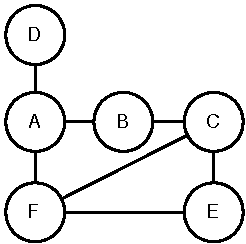
\includegraphics[bb=0bp 0bp 43mm 42mm,clip]{architecture/routing_graph}

\caption{Beispielgraph f�r ein Netzwerk}

\end{figure}



\subsubsection{Distanzvektor-Algorithmus\label{sec:distance-vector-algorithm}}

Beim Distanzvektor-Algorithmus (engl. distance vector) handelt es
sich um einen Routing Algorithmus der nach folgendem Prinzip funktioniert:
,,Teile deinen Nachbarn mit, wie du die Welt siehst''.

Dieser Algorithmus basiert darauf, dass jeder Knoten einen Vektor
verwaltet, der die Entfernungen (engl. distance) oder allgemeiner
die Gewichte zu allen �brigen Knoten enth�lt. Diese Entfernungen sind
in Wirklichkeit die Kosten. Dieser Vektor wird an die unmittelbaren
Nachbarn verteilt.

Im Detail funktioniert der Algorithmus folgenderma�en:
\begin{enumerate}
\item Am Anfang wird in jedem Knoten der Vektor folgenderma�en initialisiert.

\begin{itemize}
\item es wird eine 1 eingetragen, wenn es eine direkte Verbindung gibt und
diese nicht ausgefallen ist. Der Ausfall eines Nachbarn kann z.B.
durch regelm��ige ,,Hello'' Pakete �berpr�ft werden.
\item es wird $\infty$ eingetragen, wenn es keine direkte Verbindung gibt.
\item es wird eine 0 eingetragen, wenn es die Entfernung zu dem Router selbst
angibt.
\end{itemize}
\item Jeder Knoten sendet seinen Vektor an seine direkten Nachbarn. Es gibt
zwei verschiedene Ans�tze des Zeitpunktes wann ein Knoten seinen Vektor
an seine Nachbarn schickt:

\begin{itemize}
\item Der Knoten schickt periodisch seinen Vektor an seine Nachbarn. Die
Gr��e dieser Zeitdauer liegt im Bereich mehrerer Sekunden bis zu mehreren
Minuten.
\item Der Knoten schickt genau dann seinen Vektor an seine Nachbarn, wenn
es zu einer �nderung seines eigenen Vektors gekommen ist.
\end{itemize}
\item Empf�ngt ein Knoten einen Vektor von einem Nachbarn, dann hei�t dies,
dass der Knoten alle Knoten dieses Nachbarn �ber ihn erreichen kann.
Deshalb wird zu jeder Distanz des erhaltenen Vektors eine 1 hinzugez�hlt.
Ist der erhaltene Wert kleiner als der Wert des eigenen Vektors, dann
wird der neue Wert an Stelle des alten in den eigenen Vektor eingetragen.
Weiters wird in der Weiterleitungstabelle vermerkt, dass der Knoten
�ber diesen Nachbarn erreicht werden kann.
\end{enumerate}
Wie sieht das bei unserem Beispiel aus? Die folgende Tabelle zeigt
alle Vektoren aller Knoten im Anfangszustand:

\begin{longtable}{|c||c|c|c|c|c|c|}
\hline 
Knoten & A & B & C & D & E & F\tabularnewline
\hline
\hline 
A & 0 & 1 & $\infty$ & 1 & $\infty$ & 1\tabularnewline
\hline 
B & 1 & 0 & 1 & $\infty$ & $\infty$ & $\infty$\tabularnewline
\hline 
C & $\infty$ & 1 & 0 & $\infty$ & 1 & 1\tabularnewline
\hline 
D & 1 & $\infty$ & $\infty$ & 0 & $\infty$ & $\infty$\tabularnewline
\hline 
E & $\infty$ & $\infty$ & 1 & $\infty$ & 0 & 1\tabularnewline
\hline 
F & 1 & $\infty$ & 1 & $\infty$ & 1 & 0\tabularnewline
\hline
\end{longtable}

Jetzt beginnt das eigentliche Routing. Jeder Knoten sendet seine Vektoren
an seine direkten Nachbarn. Beispielsweise k�nnte dies so aussehen:
\begin{enumerate}
\item Knoten B erh�lt zum Beispiel einen Vektor von Knoten C. Er addiert
eine 1 zu den Gewichten der Verbindung zu C und erh�lt den Vektor
($\infty,2,1,\infty,2,2$). Dann vergleicht die Distanzen mit den
eigenen Distanzen. Ist eine Distanz kleiner, wird diese in den eigenen
Vektor �bernommen, anderenfalls kommt es zu keiner �nderung. D.h.
der Knoten B hat nach dieser Operation den Vektor (1, 0, 1, $\infty$,
2, 2) gespeichert.
\item Nehmen wir jetzt an, dass Knoten A den Vektor von Knoten B bekommt.
A aktualisiert seinen eigenen Vektor zu (0, 1, 2, 1, 3, 1).
\item Gehen wir weiter davon aus, dass Knoten A jetzt den Vektor von F bekommt.
Daher aktualisiert A seinen Vektor zu (0, 1, 2, 1, 2, 1).
\end{enumerate}
Die endg�ltigen Vektoren werden so aussehen:

\begin{longtable}{|c||c|c|c|c|c|c|}
\hline 
Knoten & A & B & C & D & E & F\tabularnewline
\hline
\hline 
A & 0 & 1 & 2 & 1 & 2 & 1\tabularnewline
\hline 
B & 1 & 0 & 1 & 2 & 2 & 2\tabularnewline
\hline 
C & 2 & 1 & 0 & 3 & 1 & 1\tabularnewline
\hline 
D & 1 & 2 & 3 & 0 & 3 & 2\tabularnewline
\hline 
E & 2 & 2 & 1 & 3 & 0 & 1\tabularnewline
\hline 
F & 1 & 2 & 1 & 2 & 1 & 0\tabularnewline
\hline
\end{longtable}

Selbstverst�ndlich muss sich jeder Knoten auch merken �ber welchen
Knoten er mittels der Distanz den Zielknoten erreichen kann. Je nach
Abfolge der Nachrichten k�nnte die Weiterleitungstabelle von Knoten
A im Prinzip so aussehen:

\begin{longtable}{|c|c|}
\hline 
Ziel & n�chster Hop\tabularnewline
\hline
\hline 
C & B\tabularnewline
\hline 
E & F\tabularnewline
\hline
\end{longtable}

Der Router muss nat�rlich auch die Schnittstellen kennen, �ber die
er die n�chsten Hops erreichen kann!

Was passiert jetzt, wenn eine Verbindung ausf�llt? Nehmen wir einmal
an die Verbindung von B nach C f�llt aus. Dann wird B an A mitteilen,
dass die Entfernung von B nach C den Wert $\infty$ ausmachen. Daraufhin
wird A seine Entfernung f�r den Weg nach C auf $\infty$ setzen, da
A das Ziel C �ber B erreicht h�tte. A w�rde diese Kosten auch an F
�bermitteln. Da F den Knoten C jedoch direkt erreichen kann, wird
F seine Kosten f�r C nicht �ndern. F w�rde im Gegenzug A mitteilen,
dass C ein direkter Nachbar von F ist und A w�rde die Kosten f�r C
auf 2 ver�ndern und dies auch B mitteilen. B wei� dann, dass C �ber
A in 3 Schritten zu erreichen ist.

Allerdings gibt es ein kleines Problem, das als Count-to-Infinity
Problem bezeichnet wird. Nehmen wir an, dass die Verbindung von A
nach D ausf�llt. A setzt daher in seinem Vektor den Wert $\infty$
f�r die Verbindung nach D ein. Nehmen wir jetzt an, dass danach eine
Aktualisierung von F kommt, die die Kosten von 2 f�r die Verbindung
nach D beinhalten. A schlussfolgert daraus, dass es den Knoten D in
3 Schritten erreichen kann und wird dies in einer weiteren Aktualisierungsmeldung
wieder an F weitergeben. F wird daraufhin seinen Vektor bez�glich
D auf 4 anpassen und diesen wieder aussenden. 

Dieser Vorgang bricht erst ab, wenn im Algorithmus die Schranke erreicht
wird, die f�r $\infty$ eingef�hrt wurde. Angenommen diese Schranke
steht bei 16, dann wird dieser Vorgang bei 16 als ,,unendlich''
abgebrochen werden. Wenn Aktualisierungen alle 20 Sekunden ausgetauscht
werden, kann es 15{*}20 Sekunden, also ca. f�nf Minuten dauern, bis
der Ausfall eines Routers erkannt und die Verbindung zu ihm als unerreichbar
markiert wird. Deshalb gibt es einige Varianten zu diesem Algorithmus.

Eine dieser Verbesserungen nennt sich Split Horizon (soviel wie geteilter
Horizont). Dabei sendet ein Knoten keine Aktualisierung an den Knoten
zur�ck von dem er einen Wert erhalten hat. In dem obigen Beispiel
w�rde F keine �nderungsmeldung bzgl. D an A schicken. Allerdings wird
A eine �nderungsmeldung an F schicken und dieser dann seinen Vektor
bzgl. D ebenfalls auf $\infty$ setzen.

Betrachten wir jetzt was passiert, wenn die Verbindung von A nach
D ausf�llt. Wenn jetzt die Aktualisierungen in einer bestimmten Reihenfolge
auftreten, kann folgendes passieren: B wei�, dass es D �ber A nicht
mehr erreichen kann, wei� aber von C, dass es D �ber C in 4 Schritten
erreichen kann und aktualisiert seinen Vektor. Gleichzeitig gibt er
diese �nderungen an A weiter. A folgert, dass es D in 5 Schritten
erreichen kann. A gibt diese �nderung wiederum an F weiter. F folgert,
dass es D jetzt in 6 Schritten erreichen kann, usw. D.h. f�r eine
Schleife, die mehr als 2 Knoten enth�lt funktioniert Split Horizon
nicht.

Eine Erweiterung zum Split-Horizon besteht darin, dass der Rechner
bei dem die Verbindung ausf�llt Meldungen mit negativen Kosten aussendet.
Solche ,,negativen'' Meldungen werden weiter verbreitet. Allerdings
werden damit keine gr��eren Schleifen als 3 vermieden.

Die Zeit, die zum Verbreiten konsistenter Routinginformationen ben�tigt
wird, wird als Konvergenzdauer oder kurz Konvergenz (engl. convergence)
bezeichnet. Der Distanzvektor Algorithmus hat eine schlechte Konvergenz.
Deshalb wurde der Link-State-Algorithmus entwickelt.


\subsubsection{Link-State-Algorithmus\label{sec:link-state-algorithm}}

Beim Link-State-Algorithmus handelt es sich um einen Routing Algorithmus
der nach folgendem Prinzip funktioniert: ,,Teile der Welt mit, wer
deine Nachbarn sind''.

Dieser Algorithmus basiert darauf, dass zuerst die Topologie des Netzes
ermittelt wird. Dann erst werden die k�rzesten Wege bestimmt.

Die Vorgehensweise von jedem Knoten ist folgende:
\begin{enumerate}
\item Jeder Knoten bildet ein LSP (link state packet, auch link state announcement,
kurz LSA, genannt) mit den Namen seiner Nachbarn und den Gewichten
der Verbindungen.
\item Der Knoten verschickt das LSP per Broadcast �ber alle seine Verbindungen.
Es werden jedoch nur die �nderungen �bertragen.
\item Der Knoten speichert alle LSP der anderen Knoten. Damit hat jeder
Knoten eine vollst�ndige Sicht des Netzes.
\end{enumerate}
Damit dies funktioniert werden zwei grundlegende Mechanismen ben�tigt:
\begin{itemize}
\item Die LSPs m�ssen zuverl�ssig alle anderen Knoten erreichen! Man nennt
das zuverl�ssiges Fluten.
\item Ein Algorithmus, der die k�rzesten Wege in dem Graphen berechnet.
Dazu wird der Dijkstra-Algorithmus verwendet.
\end{itemize}

\minisec{Zuverl�ssiges Fluten}

Damit zuverl�ssiges Fluten erm�glicht wird, muss jedes LSP folgende
Informationen beinhalten:
\begin{itemize}
\item Die Adresse des Knotens, der das LSP erzeugt hat.
\item Die Liste der direkten Nachbarn gemeinsam mit den Kosten der Verbindung.
\item Eine Sequenznummer f�r das LSP.
\item Eine Lebensdauer oder auch TTL (time to live) genannt f�r das LSP
\end{itemize}
Das Fluten funktioniert folgenderma�en:
\begin{itemize}
\item Der Austausch der LSPs wird mittels Best�tigungen und Neu�bertragungen
zuverl�ssig gemacht.
\item Jedes Mal wenn ein Knoten ein neues LSP erzeugt, wird die Sequenznummer
erh�ht. Solch eine Sequenznummer darf nicht �berlaufen. Deshalb muss
das Feld daf�r relativ gro� sein, z.B. 64 Bit. F�llt ein Knoten aus,
dann beginnt die Sequenznummer wieder von vorne.
\item Das Fluten wird mittels Broadcasts unter Ausnutzung der Sequenznummer
und der Lebensdauer realisiert:

\begin{itemize}
\item Empf�ngt ein Knoten ein LSP und es ist noch kein LSP von diesem Knoten
gespeichert, dann wird dieses gespeichert.
\item Ist schon ein LSP von diesem Knoten gespeichert, dann wird die Sequenznummer
betrachtet. Ist die neue Sequenznummer gr��er als die alte Sequenznummer,
dann wird das neue LSP gespeichert, anderenfalls wird das neue LSP
verworfen.
\item Wurde ein LSP gespeichert, dann wird die Lebensdauer des LSP dekrementiert
und dieses LSP an alle Nachbarn au�er an den Knoten von dem das LSP
empfangen wurde, weitergesendet.
\item Die Lebensdauer wird auch dekrementiert, wenn das LSP im Knoten gespeichert
ist.
\item Hat die Lebensdauer den Wert 0 erreicht, wird das LSP auf jeden Fall
gel�scht.
\end{itemize}
\end{itemize}

\minisec{Dijkstra-Algorithmus}

Jeder Knoten f�hrt den Dijkstra-Algorithmus selbstst�ndig durch. Die
Grundlage ist ein Graph, der aus den LSPs konstruiert wurde.

Wir definieren:
\begin{itemize}
\item V (engl. vertices) ist die Menge der Knoten, die durchnummeriert von
1 bis size(V) bezeichnet sind.
\item w(i,j) ist die Gewichtung der Verbindung vom Knoten i zum Knoten j.
w(i,j) = $\infty$, wenn keine Verbindung zwischen dem Knoten i und
dem Knoten j besteht.
\item Mit s wird derjenige Knoten bezeichnet, der den Algorithmus ausf�hrt.
\item Mit N wird die Menge der Knoten bezeichnet, f�r die noch kein k�rzester
Weg zu s gefunden wurde.
\item c(n) bezeichnet die Gesamtkosten vom Knoten n zum Knoten s.
\end{itemize}
Mit diesen Definitionen sieht die Grundstruktur des Dijkstra-Algorithmus
folgenderma�en aus:
\begin{lyxcode}
N~=~V~-~\{s\}

for~n~in~N:

~~~~c(n)~=~w(s,n)~~~~~~~~\#~Kosten~f�r~alle~Knoten~zu~s~initialisieren

while~not~empty(N):

~~~~w�hle~f~in~N,~sodass~c(f)~minimal~ist

~~~~N~=~N~-~\{f\}~~~~~~~~~~\#~es~ist~ein~neuer~Knoten~gefunden~worden

~~~~for~n~in~N:~~~~~~~~~~\#~Kosten~aktualisieren

~~~~~~~~c(n)~=~min(c(n),~c(f)~+~w(f,n))
\end{lyxcode}
In dieser Form werden einerseits nur die minimalen Kosten ermittelt
und au�erdem f�llt auf, dass die Wahl von f in N, sodass c(f) minimal
wird, jeweils alle Knoten in N betrachten muss. Die Idee ist, die
Menge der noch nicht behandelten Knoten weiter zu unterteilen. Es
wird die Menge der Randknoten B (engl. border) eingef�hrt, die alle
Knoten beinhaltet, die direkte Nachbarn der Knoten sind, f�r die schon
ein k�rzester Weg gefunden wurde:
\begin{lyxcode}
R~=~\{s\}~~~~~~~~~~~~~~~~~~\#~Menge~der~Ergebnisknoten~initialisieren

for~v~in~V~-~\{s\}:~~~~~~~~\#~alle~anderen~Knoten

~~~~c(v)~=~w(s,v)~~~~~~~~\#~Kosten~f�r~alle~Knoten~zu~s

~~~~p(v)~=~None~~~~~~~~~~\#~Vorg�nger~gibt~es~noch~keinen

B~=~neighbours(s)~~~~~~~~\#~mit~Nachbarn~von~s~initialisieren

for~b~in~B:~~~~~~~~~~~~~~\#~und~Vorg�nger~von~b~setzen

~~~~p(b)~=~s

while~not~empty(B):

~~~~w�hle~f~in~B,~sodass~c(f)~minimal~ist

~~~~B~=~B~-~\{f\}~~~~~~~~~~\#~aus~Rand~entfernen

~~~~R~=~R~+~\{f\}~~~~~~~~~~\#~zu~den~Gefundenen~hinzuf�gen

~~~~for~n~in~neighbours(f):

~~~~~~~~if~n~not~in~R:

~~~~~~~~~~~~B~=~B~+~\{n\}~~\#~mit~Nachbarn~zu~f~auff�llen

~~~~~~~~~~~~if~c(f)~+~w(f,n)~<~c(n):~\#~wenn~k�rzer

~~~~~~~~~~~~~~~~c(n)~=~c(f)~+~w(f,n)

~~~~~~~~~~~~~~~~p(n)~=~f
\end{lyxcode}
Praktische Implementierungen in Routern interessieren sich nicht f�r
die genauen Wege sondern nur f�r die n�chsten Router. Insoferne wird
nicht der Vorg�nger des Knotens bestimmt sondern gleich der n�chste
Router.

Folgendes Beispiel soll das verdeutlichen:

%
\begin{figure}[h]
\centering

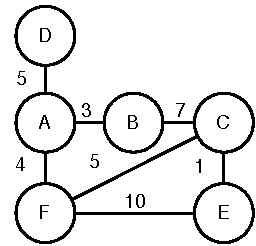
\includegraphics[bb=0bp 0bp 44mm 42mm,clip]{architecture/routing_graph2}

\caption{Beispielgraph f�r ein Netzwerk mit Gewichten}

\end{figure}


Vorausgesetzt, dass der Knoten A der Knoten ist, der den Dijkstra-Algorithmus
ausf�hrt werden folgende Schritte abgearbeitet:
\begin{enumerate}
\item Die Menge der Ergebnisknoten mit A initialisieren.
\item Randknoten bestimmen.
\item Knoten mit kleinstem Gewicht innerhalb der Randknoten bestimmen, also
B und diesen in die Menge der Ergebnisknoten �berf�hren. Neue Menge
der Randknoten bestimmen und Gewicht von C auf 10 korrigieren.
\item Knoten mit kleinstem Gewicht innerhalb der Randknoten bestimmen, also
F und diesen in die Menge der Ergebnisknoten �berf�hren. Neue Menge
der Randknoten bestimmen und Gewicht von C und E korrigieren. Gleichzeitig
wird der Vorg�nger von C der Knoten F.
\item Knoten mit kleinstem Gewicht der Randknoten bestimmen, also D und
diesen in die Menge der Ergebnisknoten �berf�hren. Menge der Randknoten
ist nicht gr��er geworden, da keine Knoten mehr vorhanden sind, die
weder in der Menge der Ergebnisknoten noch in der Menge der Randknoten
sind.
\item Knoten mit kleinstem Gewicht der Randknoten bestimmen, also C und
diesen in die Menge der Ergebnisknoten �berf�hren. Gewicht von C auf
10 korrigieren und als Vorg�nger von E den Knoten C eintragen.
\end{enumerate}
Das folgende Abbildung zeigt diese einzelnen Schritte. Die Menge der
Ergebnisknoten ist dunkelgrau und die Menge der Randknoten hellgrau
gekennzeichnet:

%
\begin{figure}[h]
\centering

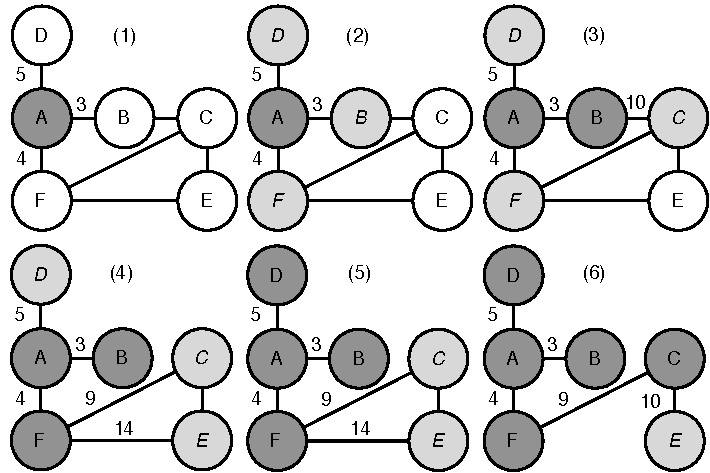
\includegraphics[bb=0bp 0bp 120mm 80mm,clip]{architecture/routing_graph2a}

\caption{Abarbeitung des Dijkstra-Algorithmus}

\end{figure}



\section{Ende-zu-Ende Kommunikation}

Ab der Schicht 4 im OSI Modell findet eine Ende-zu-Ende Kommunikation
statt, w�hrend in den Schichten 1 bis 3 jeweils eine Punkt-zu-Punkt
Kommunikation stattfindet.

Zu den Aufgaben geh�ren:
\begin{itemize}
\item Bereitstellen der Verbindungslogik.
\item Verwalten (mehrerer) Verbindungen.
\item Flusskontrolle.
\item Verwaltung von Sitzungen (engl. session).
\item Kompression und Verschl�sselung.
\item Darstellungsformatierung behandelt die Umwandlung der verschiedenen
Datenformate, sodass der Informationsgehalt jedoch unver�ndert bleibt.
Daf�r gibt es:

\begin{itemize}
\item Spezifikationen der ISO: ASN.1 (abstract syntax notation one) mittels
der Datentypen beschrieben werden k�nnen und BER (basic encoding rules),
die eine konkrete Transfersyntax beschreibt.
\item Standards des W3C (world wide web consortium): XML, XPath, XPointer,
XLink, XSLT, XML Schema
\end{itemize}
\end{itemize}

\section{�berlastkontrolle}

Obwohl die Verbindungen auf der Transportebene eine Flusskontrolle
bieten und damit den Empf�nger vor �berlastung sch�tzen, kann es vorkommen,
dass die Router auf dem Weg �berlastet werden. Zus�tzlich gibt es
noch die verbindungslosen Nachrichten�bertragungen, die ebenfalls
eine Last f�r die Router darstellen.

Folgende grunds�tzliche M�glichkeiten zum Umgang mit �berlast gibt
es:
\begin{itemize}
\item �berdimensionierung des Netzes.
\item �berlast wird aus dem Netz entfernen. Dazu muss die Netzwerksoftware
wissen welche Pakete entfernt werden sollen.
\item Neue Kommunikationsbeziehungen werden nur zugelassen, wenn gen�gend
Kapazit�ten frei sind (analog zum Telefonnetz).
\item Quelle wird gedrosselt (TCP hat ein Verfahren, dass darauf basiert)
\end{itemize}



\setpartpreamble[uc][14cm]{\vspace{3cm}In diesem Teil werden die
wichtigsten Technologien f�r LAN, WAN und Zugangsnetze vorgestellt
und im �berblick beschrieben.}


\part{Technologien}


\chapter{Ethernet\label{sec:ethernet}}

Ethernet wurde von der IEEE im Standard IEEE 802 und von der ISO als
ISO-Standard 8802 als weltweiter Standard �bernommen. Innerhalb dieses
Standards gibt es viele Teilspezifikationen, die selbst wiederum gegliedert
sind und auch andere Technologien wie Token-Ring, Token-Bus oder drahtlose
LANs enth�lt.
\begin{description}
\item [{802.2}] Logical Link Control (LLC) ist die �bertragungssteuerung
der Sicherungsschicht, die auf dem MAC Protokoll aufsetzt und damit
eine Unabh�ngigkeit von der unterliegenden �bertragungstechnologie
sicherstellt.
\item [{802.3}] Medium Access Control (MAC) -- also die Zugriffssteuerung
-- und die Spezifikation des Physical Layer (PHY) des CSMA/CD basierenden
Ethernet. Wichtige Teile sind:

\begin{description}
\item [{802.3}] 10Base-5 Ethernet basierend auf Koaxialkabel (Thick Coax).
10 gibt die �bertragungsgeschwindigkeit in MBit/s an, Base bedeutet
Basisband und 5 ist die maximale L�nge eines Segmentes in 100m (also
500m).
\item [{802.3a}] 10Base-2 Ethernet basierend auf Koaxialkabel (Thin Coax).
Die maximale L�nge eines Segmentes betr�gt hier 185m, also aufgerundet
sind das 200m. Daher kommt die Ziffer 2 in der Namensbezeichnung.
\item [{802.3u}] 100Base-TX Ethernet basierend auf Twisted-Pair Kabel und
100Base-FX basierend auf Glasfaser. Diese Art wird auch als Fast Ethernet
bezeichnet.
\item [{802.3ab}] 1000Base-T Ethernet �ber Cat-5 Kabel mit einer Distanz
bis 100m. Damit man Cat-5 Kabel verwenden kann, wurden �nderungen
am urspr�nglichen Ethernet vorgenommen. Dazu z�hlt die Verwendung
von 4 Aderpaaren anstatt von 2 wie bei Fast Ethernet.
\item [{802.3z}] 1000Base-LX bzw. 1000Base-SX Ethernet �ber Glasfaser mit
Distanzen von 440m bis zu 5km.
\item [{802.3ae}] 10GBase-xx Ethernet. Die Ziele von 10GEthernet sind,
dass es im LAN, MAN und WAN gleicherma�en einsetzbar ist und ebenfalls
(wie 1000Base-T) eine kosteng�nstige Technologie ist. Daf�r wurde
festgelegt, dass nur mehr Punkt-zu-Punkt Verbindungen im Vollduplex-Betrieb
verwendet werden und als �bertragungsmedium Glasfasern verwendet werden.
D.h., es m�ssen je Vollduplex-Verbindung zwei Glasfasern verwendet
werden. Da keine Kollisionen mehr auftreten k�nnen, ist das CSMA/CD
Prinzip nicht mehr notwendig und gro�e Link-L�ngen werden m�glich.


xx steht f�r verschiedene Varianten, die in Abh�ngigkeit der der Wellenl�nge
und der Glasfaser Distanzen von 300m bis 40km erm�glichen.

\end{description}
\item [{802.11}] Wireless LAN (WLAN). Beschreibt die Zugriffssteuerung
und den physische Schicht f�r drahtlose Netze.
\item [{802.15}] Wireless PAN. Definiert die drahtlose Kommunikation f�r
den nutzernahen Bereich �ber kurze Distanzen. Datenraten 1MBit/s bis
20MBit/s.
\end{description}

\section{Prinzip}


\subsection{CSMA/CD}

Bei den genannten Ethernet Varianten 10Base-5, 10Base-2 sowie dem
Fast Ethernet handelt es sich um eine klassische Bustopologie mit
einem Zugriffsverfahren, das auf einem Wettbewerbsverfahren basiert.
Das bedeutet, dass alle Stationen einen gemeinsamen �bertragungskanal
ben�tzen und alle Stationen gleichberechtigt sind. Die Station, die
als erstes zum Senden beginnt, darf den �bertragungskanal alleine
nutzen. D.h. die Stationen stehen in einem Wettbewerb zueinander.
Bei dem implementierten Wettbewerbsverfahren handelt es sich um CSMA/CD
(carrier sense multiple access/collision detect).

Jede Station, die nicht senden will h�rt permanent das �bertragungsmedium
ab. Erkennt es einen Rahmen (engl. frame), der an sie gerichtet ist,
wird dieser gelesen ansonsten wird der Rahmen ignoriert. Will eine
Station einen oder mehrere Rahmen senden, muss ein Algorithmus abgearbeitet
werden, da es vorkommen kann, dass zwei (oder mehrere) Stationen gleichzeitig
(engl. multiple access) zum Senden beginnen:
\begin{enumerate}
\item Eine sendebereite Station h�rt das �bertragungsmedium ab (engl. carrier
sense). Ist das �bertragungsmedium besetzt, wird gewartet bis dieses
frei ist und zus�tzlich werden noch zus�tzliche 9.6$\mu$s gewartet
(engl. interframe gap).
\item Ist das �bertragungsmedium frei, beginnt die Station zu senden.
\item Trotz �berwachung des �bertragungsmediums, kann es vorkommen, dass
zwei Stationen zur gleichen Zeit senden. Das kann vorkommen, da beide
Stationen ein freies �bertragungsmedium vorgefunden haben und deshalb
zur gleichen Zeit zu senden begonnen haben. Da die Stationen jedoch
weiter am �bertragungskanal h�ren, h�ren sie nicht ihr eigenes Signal,
sondern das �berlagerte Signal. Dieses �berlagerte Signal kennzeichnet
eine Kollision. Bei Erkennen einer Kollision (engl. collision detect)
wird von den Stationen folgendes durchgef�hrt:

\begin{enumerate}
\item Die Stationen brechen das Senden ab.
\item Die Stationen senden ein spezielles Stausignal (engl. jam signal),
damit eindeutig eine Kollision erkannt wird.
\item Danach wird eine variable Zeit gewartet (Backoff-Zeit), die mit jedem
fehlgeschlagenen Sendeversuch gr��er werden kann.
\end{enumerate}
\end{enumerate}
Damit dieser Algorithmus in dieser Form funktioniert, m�ssen -- in
Abh�ngigkeit von der Sendegeschwindigkeit und der Netzausdehnung --
bestimmte Anforderungen an die L�nge des Stausignals bzw. an die Wartezeiten
gestellt werden.

Das Flussdiagramm in Abbildung \vref{fig:CSMA/CD} zeigt den Algorithmus
in einer �bersicht.

%
\begin{figure}[h]
\centering

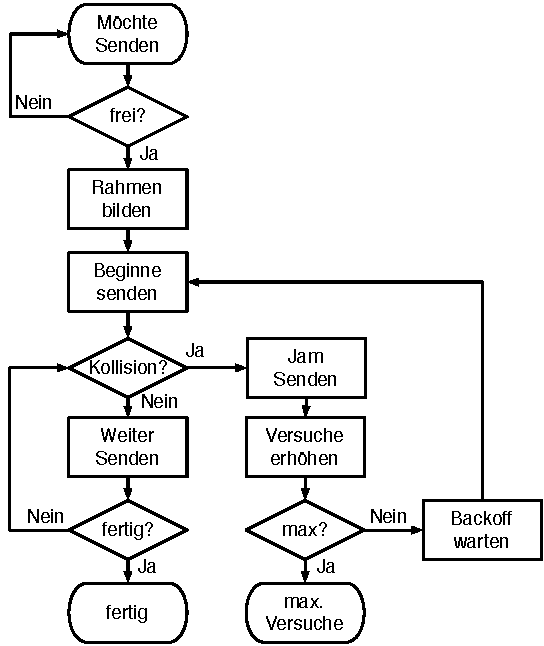
\includegraphics[bb=0bp 0bp 95mm 11cm,clip]{ethernet/csmacd_algo}

\caption{\label{fig:CSMA/CD}CSMA/CD}

\end{figure}



\subsection{Adressierung und Rahmenaufbau}

Wie im vorigen Abschnitt erl�utert, sendet eine Station Frames �ber
den Bus. Damit eine Station einen Frame an eine andere Station senden
kann, wird die Adresse dieser Station ben�tigt.


\subsubsection{MAC Adressen\label{sec:MAC_addresses}}

MAC Adressen sind f�r alle IEEE 802 Standards einheitlich definiert
und sind weltweit prinzipiell eindeutig. Diese MAC Adresse wird vom
Hersteller in einen nichtfl�chtigen Speicher der Schnittstellenkarte
(engl. network interface card, NIC) geschrieben.

Die MAC Adressen sind insgesamt 48 Bits lang setzen sich aus 3 Teilen
zusammen: 
\begin{enumerate}
\item Adresstyp bestehend aus 2 Bits (h�chstwertigste Bits, also Bit 47
und Bit 46), die angeben, ob es sich um eine Individualadresse oder
eine Gruppenadresse (Multicast-Adresse) bzw. um eine durch die IEEE
verwaltete Adresse oder eine lokal verwaltete Adresse (private Adresse)
handelt.
\item die n�chsten 22 Bits kennzeichnen den Hersteller der NIC und werden
weltweit eindeutig vergeben.
\item einem Teil, der von dem Hersteller der NIC selbst und eindeutig vergeben
wird.
\end{enumerate}
Die Adresse mit dem Wert FF-FF-FF-FF-FF-FF ist die Broadcast-Adresse.

Generell liest eine NIC nur die Frames, die an die eigene Adresse
gesendet worden sind. Allerdings kann die NIC in einen anderen Modus
geschalten werden, sodass alle Frames gelesen werden. Dieser Modus
wird promiscuos mode (dt. ausschweifend) genannt.


\subsubsection{Rahmenaufbau\label{sec:ethernet_frame}}

F�r den Aufbau eines Rahmen gibt es historisch gesehen zwei verschiedene
Arten, wobei heutzutage nur mehr die Variante von IEEE802.3 im Einsatz
ist. Die IEEE 802.3 Variante sieht folgenderma�en aus:
\begin{enumerate}
\item Pr�ambel (7 Bytes): eine alternierenden Bitfolge (also 1010...), die
der Synchronisation der Stationen dient.
\item SFD (start frame delimiter, 1 Byte): alternierende Bitfolge 10101011,
die den Start des Frame kennzeichnet.
\item Zieladresse (6 Bytes)
\item Quelladresse (6 Bytes)
\item L�ngenfeld (2 Bytes)
\item Datenblock (0 bis 1500 Bytes)
\item Pad (0 bis 46 Bytes): beinhaltet der Datenblock weniger als 46 Bytes,
dann m�ssen eine entsprechende Anzahl von Pad Bytes �bertragen werden,
sodass der Rahmen auf eine minimale Gr��e von 64 Bytes kommt.
\item FCS (engl. frame check sequence, 4 Bytes): ein CRC, der ebenfalls
vom Empf�nger berechnet wird, sodass fehlerhafte Frames einfach erkannt
und danach verworfen werden.
\end{enumerate}

\section{Netzaufbau}

Wie schon beschrieben handelt es sich bei Ethernet um eine Bus-basierte
Technologie. Bzgl. der Verkabelung gibt es allerdings zwei M�glichkeiten.
Entweder die Verkabelung wird ebenfalls als Bustopologie ausgef�hrt
(mittels Koaxialkabel) oder sternartig wie bei Twisted-Pair Kabeln
bzw. bei Glasfaserkabeln.


\subsection{Bustopologie mit Koaxialkabel}

Fr�her eingesetzte Ethernet Technologien sind 10Base-5 bzw. 10Base-2,
die auf Koaxialkabeln basieren (siehe \vref{sec:coaxial_cable}).
Ein Segment besteht aus einem langen Kabel, das an beliebigen Stellen
entweder angebohrt (10Base-5) bzw. mittels BNC Steckverbindungen (10Base-2)
den Anschluss von Arbeitstationen erm�glicht. Mehrere Segmente k�nnen
mittels Repeater oder Br�cken zusammengeschlossen werden.

Auf Grund der technischen Spezifikationen mussten folgende Bedingungen
eingehalten werden, die unter der 5-4-3 Regel bekannt waren: Zwischen
je zwei Endger�ten d�rfen maximal 5 Segmente und 4 Repeater liegen.
Nur an 3 Segmenten ist der Anschluss von Arbeitsstationen erlaubt.


\subsection{Sterntopologie mit Twisted-Pair Kabel bzw. Glasfaser}

Heute wird haupts�chlich die Sterntopologie verwendet. Es werden die
Arbeitstationen sternf�rmig mit Kopplungselementen (siehe \vref{sec:coupling_devices})
verbunden. Bei den Kopplungsger�ten handelt es sich haupts�chlich
um Hubs, Bridges und Switches. In dieser Konfiguration wird die Ethernet
Technologie im Zuge der strukturierten Verkabelung eingesetzt (siehe
\vref{sec:structured_cabeling}).


\section{Spanning-Tree-Algorithmus}

Der Backward-Learning Algorithmus (siehe \vref{sec:coupling_devices})
hat allerdings ein Problem sobald Schleifen in der Netzstruktur vorhanden
sind. Schleifen entstehen, wenn redundante Pfade vorhanden sind. Solche
redundante Pfade werden gerne verwendet, um die Verf�gbarkeit des
Netzes zu erh�hen.

Das Problem l�sst sich folgenderma�en beschreiben: Durch das Fluten
in einer Schleife werden Frames im Kreis gesendet und es ensteht eine
unn�tige Last. Ist der Zielhost im Netz vorhanden, dann wird dieser
eine Antwort schicken und die Switches k�nnen sich im Zuge des Backward-Learning
auch die Ziel-Adresse merken, wodurch das Fluten ausbleibt und die
Frames nicht mehr im Kreis gesendet werden. Ist der Zielhost allerdings
nicht im Netz verf�gbar ist, dann kreisen die Frames in der Schleife.
Genauso ist problematisch wie fehlende Zielhosts ist, wenn Broadcast-
oder Multicast-Frames verschickt werden, da kreisende Frames auch
nicht durch Antworten der Zielhosts entfernt werden.

Eine einfache M�glichkeit, die von Switches implementiert wird ist,
dass diese automatisch einen Port abschalten, wenn die Auslastung
auf diesen Port zu hoch (z.B. gr��er als 90\%) wird. Die Argumentation
ist, dass ein solch hohes Verkehrsaufkommen im normalen Betrieb nicht
auftritt und deshalb vermutlich kreisende Frames die Ursache sind.

Die bessere L�sung, die redundante Verbindungen erst erm�glicht ist
die Implementierung des Spanning Tree Protocol (STP, IEEE802.1). Das
Ziel dieses Verfahrens ist, eine schleifenlose Topologie aufzubauen
(einen Baum), die alle Switches einbindet und die redundanten Verbindungen
deaktiviert. Stellt man sich das LAN als einen Graphen vor, der Zyklen
enth�lt, dann wird durch den STP ein zyklenloser Graph generiert,
der alle Zielhosts enth�lt. Eine Lastverteilung ist in diesem Fall
nicht mehr m�glich.

Jeder Switch hat einen eindeutigen Identifier und tauscht mit den
anderen Switches im Zuge des STP Konfigurationsnachrichten aus. Der
prinzipielle Ablauf von STP sieht folgenderma�en aus:
\begin{enumerate}
\item Es wird der Switch mit dem kleinsten Identifier als Wurzel des Baumes
festgelegt. Eine Wurzel leitet Frames prinzipiell an alle ihre Ports
weiter (d.h. keiner der Ports ist deaktiviert).
\item Dann berechnet jeder Switch den k�rzesten Weg zur Wurzel und merkt
sich den Port, der zur Wurzel f�hrt.
\item Alle an ein Segment angeschlossene Switches w�hlen einen designierten
Switch, der alle Nachrichten aus diesem Segment an die Wurzel weiterleitet.
Es wird derjenige Switch gew�hlt, der den kleinsten Weg zur Wurzel
hat. Gibt es mehrere Switches mit dem kleinsten Weg, dann wird wieder
derjenige ausgew�hlt, der von diesen den kleinsten Identifier besitzt.
D.h. derjenige Switch, der nicht als designierter Switch festgelegt
wurde, deaktiviert seinen Port Richtung Wurzel.
\item Ist der Prozess abgeschlossen, dann sendet nur mehr die Wurzel Konfigurationsnachrichten
aus, die von allen Switches weitergeleitet werden. Enth�lt ein Switch
innerhalb einer gewissen Zeitspanne keine Konfigurationsnachricht,
wird angenommen, dass ein Switch ausgefallen ist und der Prozess beginnt
wieder von vorne.
\end{enumerate}
In Abbildung \vref{fig:stp_ex} ist ein Beispiel eines Netzes als
Graph zu sehen, in dem die deaktivierten Ports strichliert markiert
sind. Als Wurzel wurde S1 bestimmt.

%
\begin{figure}[h]
\centering

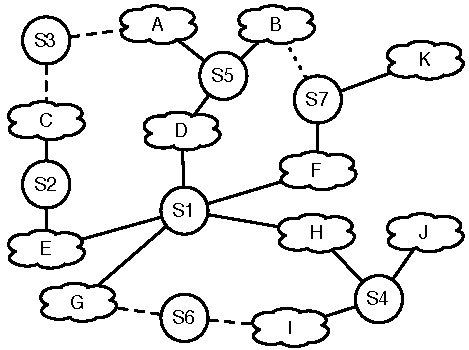
\includegraphics[bb=0bp 0bp 80mm 60mm,clip]{ethernet/stp_ex}

\caption{\label{fig:stp_ex}Beispiel eines Netzes mit durch STP deaktivierten
Ports}

\end{figure}




\chapter{WLAN}

Heute wird unter WLAN (wireless LAN) meist die in IEEE 802.11 beschriebene
Technologie verstanden. Diese ist f�r den Aufbau drahtloser Netze
innerhalb eines begrenzten geographischen Bereich (Haushalte, B�rogeb�ude,
Firmengel�nde) ausgelegt.


\section{Prinzip}

In IEEE 802.11 sind zwei �bertragungstechniken mittels Funk im Spreizspektrumverfahren
bei dem das Signal auf ein breiteres Frequenzband ausgedehnt (gespreizt)
wird, um die Auswirkungen von St�rungen durch andere Ger�te zu minimieren:
\begin{itemize}
\item Frequenzsprungverfahren (engl. frequence hopping): es wird das Signal
auf ein st�ndig die Frequenz wechselndes Tr�gersignal moduliert. Die
Auswahl der Frequenz finden pseudozuf�llig mittels eines Pseudozufallszahlen-Generators
statt. Sowohl Sender als Empf�nger initialisieren ihren Pseudozufallszahlen-Generator
gleich.
\item Direct Sequence: Dieses Spreizspektrumverfahren basiert darauf, dass
jeder Teilnehmer einen Code (wieder eine Pseudozufallfolge) erh�lt
mit der er seinen eigentlichen Bitstrom verkn�pft. Damit wird das
Signal auf eine relativ gro�e Bandbreite gespreizt. Alle Sender belegen
die selbe Bandbreite. Der Empf�nger verwendet wieder die selbe Pseudozufallsfolge
und kann dadurch das Signal wieder rekonstruieren. In IEEE 802.11
wird eine 11 Bit lange Folge f�r jedes Bit in dem urspr�nglichen Signal
verwendet.
\end{itemize}
Die dritte �bertragungstechnik basiert auf Infrarot�bertragung und
ist auf ca. 10m Reichweite begrenzt. Sender und Empf�nger m�ssen nicht
direkt aufeinander ausgerichtet sein.

Mit den Funk-basierten Verfahren lassen sich �bertragungsraten im
Bereich von 11MBit/s bis 54MBit/s erzielen. Der neue Standard IEEE
802.11n, der derzeit als Draft vorliegt erlaubt Datenraten bis 540MBit/s
(eine endg�ltige Version des Standard wird f�r 2008 erwartet).


\section{Kollisionsvermeidung}

Das Verfahren von IEEE802.11 ist �hnlich dem CSMA/CD Verfahren von
Ethernet, jedoch kann keine Kollisionserkennung durchgef�hrt werden.
Lediglich eine Kollisionsvermeidung l�sst sich erzielen. Das liegt
daran, dass nicht jeder Knoten in der Reichweite der anderen befindet.
Zwei Probleme treten auf:
\begin{labeling}{00.00.0000}
\item [{Verborgene~Knoten}] (engl. hidden node) Es kann prinzipiell vorkommen,
dass es zu Kollisionen kommt, diese jedoch nicht erkannt werden (siehe
nachfolgende Abbildung; die Umgebung von B und D ist der �bersichtlichkeit
halber grau eingezeichnet). Angenommen A und C m�chten mit B kommunizieren
und senden je einen Frame. A und C k�nnen die Kollision bei B nicht
erkennen! D.h. A und C sind f�r einander verborgene Knoten.


\begin{center}
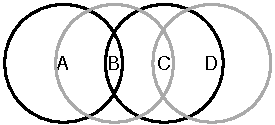
\includegraphics[bb=0bp 0bp 47mm 22mm,clip]{wlan/hidden_nodes}
\par\end{center}

\item [{Exponierte~Knoten}] (engl. exposed node) Angenommen B sendet an
A. Knoten C wei� von der Kommunikation, allerdings w�re es f�r C falsch
anzunehmen, dass C an niemanden �bertragen darf, nur weil C die Kommunikation
an A bemerkt. C k�nnte ohne Probleme an D senden.
\end{labeling}
In IEEE 802.11 sind zwei prinzipiell verschiedene Methoden definiert
wie diese Probleme gel�st werden:
\begin{labeling}{00.00.0000}
\item [{RTS/CTS}] funktioniert folgenderma�en: Sender und Empf�nger tauschen
zus�tzliche Nachrichten aus, um festzulegen wer senden darf. Bevor
ein Sender senden will sendet dieser ein RTS (request to send) Frame
an den Empf�nger. Der Empf�nger antwortet mit einem CTS (clear to
send) Frame. CTS reicht das L�ngenfeld an den Sender zur�ck. Sieht
ein anderer Knoten den CTS Frame, wei� er, dass er nahe beim Empf�nger
liegt und daher solange nicht �bertragen kann, bis ein Frame mit der
spezifizierten L�nge �bertragen wurde. Ein Knoten, der zwar den RTS
aber nicht den CTS sieht befindet sich nicht nahe genug am Empf�nger,
um diesen zu st�ren, sodass er nach Belieben �bertragen kann. Au�erdem
sendet der Empf�nger nach dem Erhalt der Nachricht ein ACK an den
Sender. Alle Stationen m�ssen auf dieses ACK warten bis sie �bertragen
k�nnen. Zwei RTS Signale k�nnen trotzdem am �bertragungskanal kollidieren.
Da solch eine Kollision nicht erkannt werden kann, nimmt der Sender
an, dass eine Kollision aufgetreten ist, wenn innerhalb einer gewissen
Zeitspanne kein CTS erkannt wird und sendet nach einer gewissen Zeitdauer
wieder (wie bei Ethernet).
\item [{PCF}] (point coordination function) Der Zugangspunkt (siehe Abschnitt
\vref{sec:wlan_netstructure}) ist der einzige, der spontan senden
darf und fragt alle Stationen permanent ab (polling), ob sie etwas
senden wollen. Es handelt sich also um eine zentrale Zuteilung. Dadurch
werden Kollisionen vermieden.
\end{labeling}

\section{Netzaufbau\label{sec:wlan_netstructure}}

IEEE 802.11 Netze k�nnen entweder als Infrastrukturnetze oder als
Ad-hoc-Netze aufgebaut werden. Ein Infrastrukturnetz liegt vor, wenn
die Teilnehmer �ber feste Zugangspunkte (engl. access point, AP) kommunizieren.
Ad-hoc-Netze ben�tigen keine Infrastruktur, d.h. die Teilnehmer kommunizieren
direkt miteinander und steuern den Ablauf der Kommunikation.

Bei einem Infrastrukturnetz mit mehreren APs sind diese mittels eines
Verteilnetzes miteinander verbunden. Jeder Knoten meldet sich bei
einem AP an, indem er einen Probe-Frame sendet (aktives Scanning),
der von jedem AP beantwortet, der in der Umgebung des Knoten liegt.
Der Knoten w�hlt sich darauf hin einen der AP aus. Alternativ dazu
gibt es die M�glichkeit, dass der AP von sich aus in regelm��igen
Abst�nden sogenannte Beacon-Frames (dt. Bake) aussendet (passives
Scanning) und seine Pr�senz als auch die von ihm unterst�tzten �bertragungsraten
bekannt gibt.


\section{Alternative Technologien}


\subsection{Bluetooth}

Bluetooth (IEEE 802.15.1) ist eine andere funkbasierte Technologie
mit Schwerpunkt der Vernetzung von Ger�ten �ber eine kurze Distanz
(je nach Sendeleistung von 10m bis 100m). Es wurde als solches f�r
den Einsatz als PAN konzipiert und wird deshalb auch zur Vernetzung
von Handys, PDAs, Computer oder Peripherieger�ten verwendet. F�r diese
Anwendungen unterst�tzt es Daten und Sprache und auch eine Verschl�sselung.

Um f�r diese Einsatzgebiete verwendbar zu sein, wurde es von Haus
aus als kosteng�nstige Technik entworfen und verwendet auch das weltweit
verf�gbare ISM (Industrial, Scientific and Medical Band) im 2.4GHz
Band. Es erm�glicht Datenraten bis 700KBit/s im Download und gleichzeitig
57KBit/s im Upload. In der erweiterten Variante werden Datenraten
bis 2.1MBit/s unterst�tzt.


\subsection{IrDA}

Die IrDA-Schnittstelle (Infrared Data Association) basiert auf einer
gerichteten Sichtverbindung mit infrarotem Licht und hat die Zielstellung
Kabelverbindungen zu ersetzen. Die Verbindung ist auf eine Entfernung
von 2m begrenzt und erm�glicht halbduplex eine Datenrate von 115KBit/s.
In der Version 1.1 der IrDA Spezifikation ist eine Datenrate von 4MBit/s
m�glich.


%
\chapter{Tokenring}

Die Tokenring Technologie wurde urspr�nglich von IBM entwickelt und
ist in IEEE 802.5 spezfiziert. Urspr�nglich waren entweder 4MBit/s
(Ringl�nge max. 360m) bzw. 16MBit/s (Ringl�nge max. 168m) Datenrate
m�glich. Bez�glich der �bertragungsleistung entspricht dies in etwa
der �bertragungsleistung eines Ethernet-Netzes mit 10MBit/s bzw. 100MBit/s.
Aktuelle Weiterentwicklungen sind z.B. die GBit-Variante (IEEE 802.5v),
ein Konzept zur Realisierung von VLANs bzw. das Konzept der Link Aggregation.
Link Aggregation bedeutet die Verbindung zweier Switches durch parallele
Links zur Erh�hung der Bandbreite.


\section{Prinzip}

Das Konzept besteht darin, dass ein logischer Ring der Arbeitsstationen
gebildet wird. In diesem Ring wird ein Token (dt. Marke) im Kreis
geschickt. Solange keine Station senden will, kreist ein Frei-Token.
Will eine Station senden, nimmt es das Token aus dem Ring und ersetzt
es durch ein Besetzt-Token und h�ngt die Daten und die Adresse an
und schickt das Token wieder in den Ring. Kommt das Token beim Empf�nger
an, wird das Token von diesem kopiert und wieder in den Ring eingespeist.
Erst der Sender entnimmt das Token aus dem Ring und ersetzt es wieder
durch ein Frei-Token. Jeder Sender darf maximal f�r die Dauer der
THT (token holding time) senden (typisch 10ms), danach muss er ein
Frei-Token weitergeben.

Es gibt also keine ausgezeichnete Station, die den Zugriff steuert.
D.h. der Tokenring verwendet ein dezentrales Zuteilungsverfahren.
Zur �berwachung des Ringes wird eine Station als aktiver Monitor bestimmt,
w�hrend andere Stationen als passive Monitore (standby monitors) agieren
k�nnen, die bei Ausfall des aktiven Monitors selbst aktiv werden.


\section{Netzaufbau}

Die Stationen werden aktiv in den Ring eingef�gt. Sie empfangen und
regenerieren das am Eingang ankommende Signal, werten es aus und geben
es regeneriert am Ausgang weiter. F�llt eine Station aus oder wird
sie ausgeschaltet, w�rde allerdings der Ring unterbrochen werden.
Um dies zu verhindern, werden die Stationen \emph{sternartig} an einen
Ringleitungsverteiler, genannt auch MSAU (multi station access unit)
in den Ring eingef�gt.

In jeder MSAU sind Schalter eingebaut, die bei Ausfall oder Abschaltung
einer Station diese �berbr�cken und dadurch den Ring wieder herstellen.
D.h. z.B., dass die Verkabelung sternartig durchgef�hrt wird, aber
das Netz logisch als Ring arbeitet.


%
\chapter{FDDI}

FDDI (Fiber Distributed Data Interface) weist gro�e �hnlichkeiten
mit dem Tokenring auf. Die Datenrate ist 100MBit/s. Es gibt auch eine
Variante mit einer Datenrate von 1000MBit/s. Ringl�ngen sind bis zu
100 oder 200km m�glich.


\section{Prinzip}

In Abweichung zum Tokenring werden optische Fasern in einem Doppelring
verwendet. Bei FDDI kreist ebenfalls ein Token im Kreis, im Unterschied
zum Tokenring k�nnen jedoch auch mehrere Tokens gleichzeitig kreisen.
Dazu gibt der Sender das Token sofort nach dem Senden des letzten
Frames wieder frei. Das Entfernen der Rahmen wird ebenfalls nur vom
Absender durchgef�hrt.


\section{Netzaufbau}

Der Doppelring besteht aus zwei Ringen, die gegel�ufig betrieben werden
und als Haupt- und Ersatzring ausgelegt sind. Bei einer Unterbrechung
beider Ringe (an der selben Stelle) k�nnen die benachbarten Stationen
den Ring wieder schlie�en. Damit wirkt sich die Unterbrechung, abgesehen
von einer doppelt langen Ringl�nge nicht aus.

�hnlich den MSAUs im Tokenring definiert der FDDI Standard ebenfalls
Anschlussm�glichkeiten f�r die einzelnen Stationen. Allerdings werden
verschiedene Arten von Stationen definiert:
\begin{itemize}
\item Eine DAS (dual attachment station) verf�gt �ber zwei getrennte Anschl�sse,
sodass die Station unabh�ngig �ber beide Ringe kommunizieren kann.
Ebenfalls wie bei Tokenring wird bei Ausfall der Station der Ring
nicht unterbrochen.
\item Ein DAC (dual attachment concentrator) wird wie eine DAS an den Ring
angeschlossen. Das Besondere ist, dass an einen DAC mehrere DAS bzw.
SAS (siehe n�chsten Punkt) angeschlossen werden k�nnen.
\item Eine SAS (single attachment station) wird immer �ber eine DAS oder
DAC an den Ring angeschlossen.
\end{itemize}
DAC bzw. DAS sind direkt im Doppelring einh�ngbar. Eine SAS kann nicht
direkt in den Doppelring eingeh�ngt werden. Eine DAS kann auch an
zwei verschiedene DAC angeschlossen werden. Diese als Dual Homing
bezeichnete Konfiguration und erh�ht nochmals die Verf�gbarkeit der
Station am Netz.


%
\chapter{WAN Technologien}

In diesem Kapitel werden die wichtigsten WAN Technologien kurz vorgestellt.


\section{X.25}

Bei X.25 handelt es sich um ein �ffentliches, paketvermittelndes Netzwerk,
das im Jahr 1976 standardisiert wurde. Eigentlich beschreibt X.25
die Schnittstelle zwischen Endger�t und Netz. X.25 Netze stellen permanente
virtuelle Verbindungen oder geschaltete virtuelle Verbindungen zur
Verf�gung. An Datenraten sind 300Bit/s bis 64KBit/s definiert und
seit 1992 gibt es auch 2MBit/s. Die Datenraten entsprechen nicht mehr
den heutigen Anforderungen an ein WAN. Der Grund f�r die niedrigen
Datenraten liegt einerseits darin, dass die Technologie relativ alt
ist und X.25 f�r die Verwendung �ber schlechte analoge �bertragungsstrecken
ausgelegt wurde. Der gro�e Vorteil dieser Technologie ist, dass sie
weltweit verf�gbar ist.


\section{ISDN}

ISDN steht f�r Integrated Services Digital Network und hat das Ziel,
verschiedene Dienste wie Sprach-, Daten- und Bildkommunikation in
einem Netz zur Verf�gung zu stellen. Es wurde im Jahr 1984 standardisiert
und ist ebenfalls ein �ffentliches, aber leitungsvermitteltes Netz.
Prinzipiell gibt es zwei Arten von Anschl�ssen:
\begin{itemize}
\item Der Basisanschluss (Basic Rate Interface, BRI) fasst zwei B Kan�le
und einen D-Kanal zusammen. Ein B-Kanal hat eine Datenrate von 64KBit/s
und ein D-Kanal eine Datenrate von 16KBit/s. B-Kan�le sind Datenkan�le
und der D-Kanal ist als Signalisierungskanal vorgesehen (Steuerung).
\item Der Prim�rmultiplexanschluss (Primary Rate Interface, PRI) fasst 30
B-Kan�le und einen D-Kanal zusammen.
\end{itemize}

\section{Frame Relay}

Bei Frame Relay handelt es sich um eine Weiterentwicklung von X.25.
Dazu kann es einerseits als abgemagerte Variante von X.25 betrachtet
werden, die h�here Datenraten unterst�tzt (bis zu 45MBit/s sind machbar).
Das ist deshalb m�glich, da X.25 f�r �bertragungsstrecken mit hohen
Fehlerraten ausgelegt war und deshalb aufw�ndige Protokolle f�r die
sichere �bertragung beinhaltet. Durch die wesentlich geringeren Fehlerraten
auf neueren digitalen �bertragungssystemen k�nnen einfachere Protokolle
verwendet werden. Charakteristisch ist, dass Pakete im Vergleich zu
ATM eine variable L�nge aufweisen.


\section{ATM}

ATM (asynchronous transfer mode) ist eine verbindungsorientierte,
die eine eine Bereitstellung von Dienstg�ten zur Verf�gung stellt.
ATM wurde 1986 standardisiert und wird haupts�chlich von Netzbetreibern
im WAN Bereich eingesetzt. Im LAN hat es sich nicht durchgesetzt und
mit der Einf�hrung von 10-Gigabit-Ethernet wird vermutet, dass ATM
auch im WAN (teilweise) abgel�st wird, da die Hardware relativ aufw�ndig
ist und auch eine umfassende Administration des Netzes notwendig ist.

Auch bei ATM k�nnen entweder permanente virtuelle Verbindungen (in
etwa wie Standleitungen) oder transiente virtuelle Verbindungen (in
etwa wie W�hlleitungen) aufgebaut werden. Eine Verbindung wird bei
ATM nur aufgebaut, wenn die geforderten G�teklassen erf�llt werden.
Bei ATM handelt es sich um eine zellenbasierte Technologie. Unter
einer Zelle versteht man ein kleines Paket mit fester Gr��e. Die Daten
werden dazu in Paket je 48 Bytes unterteilt und mit 5 Bytes Header
versehen. Der Vorteil solcher Pakete liegt darin, dass der Jitter
klein ist. ATM unterst�tzt derzeit Datenraten bis zu 625MBit/s.


\section{Zugangsnetze}

Als leitungsgebundene Zugangsnetze bzw. Zugangsverfahren sind in Verwendung:
Modemverbindung �ber Telefonleitung, ISDN Anschluss, xDSL (digital
subscriber line), Modem �ber Kabelnetz sowie die Mitverwendung der
Stromversorgungsleitungen.

F�r den leitungsungebundenen Zugang werden Mobilfunk �ber GSM, Mobilfunk
�ber UMTS, Richtfunk und Satellitenfunk eingesetzt. In der Zukunft
werden weitere Funktechnologien folgen, z.B.: Wimax (worldwide interoperability
for microwave access), ein Funkstandard f�r Breitbandanbindungen bis
zu 70MBit/s und bis zu 50km.


\setpartpreamble[uc][14cm]{\vspace{3cm}Dieser Teil beschreibt den
,,defacto'' Standard TCP/IP in solch einem detailierten Niveau wie
f�r das Verst�ndnis von Rechnernetzen notwendig.}


\part{TCP/IP\label{par:tcpip}}


\chapter{�berblick und Struktur von TCP/IP}

TCP/IP ist bez�glich der Funktionen ebenfalls in Schichten aufgeteilt,
auch wenn die Schnittstellen zwischen den Schichten (im Gegensatz
zum ISO/OSI Modell) nicht definiert sind. Es wird oft eine Abbildung
der Schichten vom TCP/IP Stack zum OSI Modell vorgenommen. Auf der
untersten Ebene gibt es wieder die Bit�bertragungsschicht, dar�ber
die Sicherungsschicht, dar�ber die Vermittlungsschicht und zum Schluss
die Transportschicht. Dar�ber hinaus gibt es nur noch eine Anwendungsschicht
und die eigentlichen Anwendungen.
\begin{itemize}
\item D.h. der TCP/IP Protokollstack l�sst sich in diesem Sinne als ein
Schichtenmodell von 4 Schichten beschreiben, die jeweils 4 Schichten
im ISO/OSI Referenzmodell zugeordnet werden k�nnen:
\item Als unterste Schicht dient die Verbindungsschicht (engl. auch network
interface layer genannt), die die Bit�bertragungsschicht \emph{und}
die Sicherungsschicht des ISO/OSI Modells umfasst.
\item Darauf baut die Internetschicht (engl. internet layer) auf, die der
Vermittlungsschicht im ISO/OSI Modell entspricht. In dieser Schicht
gibt es in TCP/IP die Protokolle Internet Protocol (IP), Internet
Control Message Protocol (ICMP), das Address Resolution Protocol (ARP)
und das Reverse Address Resolution Protocol (RARP).
\item Die n�chste Schicht ist die Transportschicht (engl. transport layer),
die wiederum direkt auf die Transportschicht im ISO/OSI Modell abgebildet
werden kann. Im TCP/IP Modell gibt es zwei verschiedene Transportprotokolle:
Transport Control Protocol (TCP) und User Datagram Protokoll (UDP).
\item Als n�chste Schicht folgt im TCP/IP Modell direkt die Anwendungsschicht,
die hiermit auch die Funktionen der Sitzungsschicht und der Darstellungsschicht
beinhalten muss. F�r diese beiden Schichten des ISO/OSI Modells gibt
es in TCP/IP kein Gegenst�ck.
\end{itemize}
Die Abbildung \vref{fig:tcpip_layers} stellt die Schichten und die
Querverbindungen dar. Es ist daraus auch zu erkennen, dass das TCP/IP
Modell eigentlich kein striktes Schichtenmodell implementiert.

%
\begin{figure}
\centering

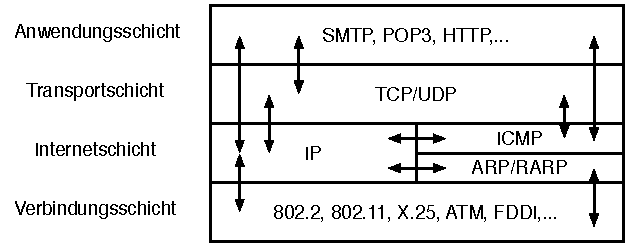
\includegraphics[bb=0bp 0bp 138mm 42mm,clip]{tcpip_overview/tcpip_layers}

\caption{\label{fig:tcpip_layers}TCP/IP Schichtenmodell}

\end{figure}


Man sieht, dass in der Verbindungsschicht nicht nur IP (der eigentliche
Kern von TCP/IP) angesiedelt ist, sondern noch weitere Protokolle,
die nicht direkt zu IP geh�ren, jedoch ein integraler Bestandteil
dieser Schicht sind. Dies ist einerseits ICMP, das haupts�chlich zur
Benachrichtigung von Fehlern in der Internetschicht dient und die
Protokolle ARP und RARP, die zur Umsetzung von IP Adressen in Hardwareadressen
(wie z.B. Ethernet-MAC-Adressen) bzw. umgekehrt dienen.

Der Hauptzweck der Internetschicht liegt in der globalen Adressierung
der Hosts und der �bertragung der Pakete zwischen den Hosts.

In der Transportschicht gibt es zwei Protokolle, n�mlich das verbindungsorientierte,
zuverl�ssige TCP und das verbindungslose, unzuverl�ssige UDP.

Die Anwendungsschicht ist in den eigentlichen TCP/IP Standards nicht
beschrieben und muss, wie schon erw�hnt, ebenfalls die Funktionen
der Sitzungsschicht und der Darstellungsschicht �bernehmen. D.h. obwohl
der TCP/IP Protokollstack vom Prinzip her ebenfalls eine Anwendungsschicht
vorsieht, es jedoch keinen Standard gibt, ist jede Anwendung aus diesem
Grund daf�r selbst zust�ndig die ben�tigten Funktionen der Sitzungsschicht,
der Darstellungsschicht und der Anwendungsschicht zu implementieren.

Die Protokolle IP, TCP, UDP, ICMP und ARP werden in weiterer Folge
noch genauer beschrieben.



\chapter{Internet Protokoll\label{sec:ip}}

Das Internet Protokoll (IP) ist der Kern des TCP/IP Stacks. Derzeit
ist die Version 4 (IPv4) beschrieben im RFC 791 aus dem Jahr 1981
fl�chendeckend im Einsatz. Weitere relevante RFCs sind 950, 919 and
922 und RFC 2474. 

Bei IP handelt es sich um ein verbindungsloses Protokoll auf der Schicht
3, dessen Hauptfunktionen in der Bereitstellung der Adressierung,
der Weiterleitung und der Abstraktion der unterliegenden physikalischen
Schicht liegt.

Es handelt sich bei IP um ein nicht zuverl�ssiges Protokoll, das nach
dem best-effort Prinzip arbeitet. Das bedeutet, dass versucht wird
die Pakete so gut wie m�glich zuzustellen. Trotzdem k�nnen Pakete
verloren gehen, nicht in der richtigen Reihenfolge ankommen oder auch
mehrfach ankommen. IP geht davon aus, dass die h�heren Schichten sich
um diese Punkte k�mmern.


\section{IP Adressen}

Die IP Adresse dient dazu, Hosts auf der Vermittlungsschicht eindeutig
ansprechen zu k�nnen und die Wegewahl von IP-Paketen zwischen Sender
und Empf�nger zu unterst�tzen. 

In IPv4 besteht jede Adresse aus genau 32 Bits, die meist in 4 Bytes
angeschrieben werden. Die Bytes werden in der Darstellung durch je
einen Punkt getrennt und in dezimaler Zahlendarstellung angegeben.

IPv4 unterteilt die Adressen in Unicast-, Multicast- und Broadcastadressen.
Zus�tzlich bietet IPv4 insgesamt 3 Arten von Adressierungsvarianten:
Standardadressen, Subnetzadressen und das sogenannte Classless Inter-Domain
Routing (CIDR).

Prinzipiell besteht jede Adresse aus einem Netzanteil und einem Hostanteil.
Der Netzanteil identifiziert das Netz und der der Hostanteil gibt
den Host innerhalb des Netzes an. Der Grund f�r diese Einteilung liegt
in der Notwendigkeit der Weiterleitung!


\subsection{Standardadressen\label{sec:standard_ip_addresses}}

Bei den Standardadressen gibt es 4 Hauptadressklassen und eine Klasse,
die f�r zuk�nftige Anwendungen vorgesehen ist:
\begin{labeling}{00.00.0000}
\item [{Klasse~A}] Diese Klasse ist f�r eine hohe Anzahl an Hosts vorgesehen.
Der Netzanteil ist jeweils das erste Byte einer Adresse, wobei das
erste Bit einer solchen Adresse ist immer 0 ist. Daraus ergibt sich
ein theoretischer Adressbereich von 0.0.0.0 bis 127.255.255.255. Die
Netze 0.0.0.0 und 127.0.0.0 sind jedoch reserviert, sodass es 126
verschiedene Klasse A Netze gibt. Je Klasse A Netz gibt es maximal
16.777.214 ($2^{24}-2$) Hosts. Der Grund warum 2 abgezogen werden
muss und warum die Netze 0.0.0.0 und 127.0.0.0 ebenfalls nicht zur
Verf�gung stehen wird im Abschnitt \vref{sec:special_ip_addresses}
und im Abschnitt \vref{sec:reserved_ip_addresses} beschrieben. Der
effektive, nutzbare Bereich geht also von 1.0.0.1 bis 126.255.255.254.
\item [{Klasse~B}] Klasse B Netze sind f�r eine mittlere Anzahl an Hosts
vorgesehen. Der Netzanteil sind die beiden ersten Bytes, wobei die
ersten beiden Bits immer 10 sind. Daraus ergibt sich ein theoretischer
Adressbereich von 128.0.0.0 bis 191.255.255.255. Insgesamt sind so
16384 ($2^{14}$) verschiedene Klasse B Netze m�glich. Je Klasse C
Netz gibt es maximal 65534 ($2^{16}-2$). Der effektive Bereich ergibt
sich zu 128.0.0.1 bis 191.255.255.254.
\item [{Klasse~C}] Klasse C Netze sind f�r eine kleine Anzahl an Hosts
vorgesehen. Der Netzanteil sind die ersten drei Bytes, wobei die ersten
drei Bits immer 110 sind. Daraus ergibt sich ein theoretischer Adressbereich
von 192.0.0.0 bis 223.255.255.255. Insgesamt sind so 2097152 ($2^{21}$)
verschiedene Klasse C Netze m�glich. Je Klasse C Netz gibt es maximal
254 ($2^{8}-2$) Hosts. Der effektive Bereich ergibt sich zu 192.0.0.1
bis 223.255.255.254.
\item [{Klasse~D}] Klasse D Netzadressen sind f�r Multicast-Anwendungen
reserviert. Die ersten vier Bits sind immer 1110 und die restlichen
28 Bits geben die Multicast-Gruppen-Id an. Der theoretische Adressbereich
geht von 224.0.0.0 bis 239.255.255.255. Von diesen sind jedoch einige
vordefiniert, wie z.B. wieder 224.0.0.0 als reservierte Basisadresse,
224.0.0.1 f�r alle Hosts in dem Subnetz und weitere.
\item [{Klasse~E}] Diese Klasse ist f�r zuk�nftige Anwendungen rerserviert.
Solche Adressen beginnen mit 11110.
\end{labeling}
Die Gr�nde f�r den Aufbau der Adressen sind, dass
\begin{itemize}
\item durch diese Einteilung die Eintr�ge in den Routern minimiert werden
k�nnen. Daher kommt es auch, dass den einzelnen geographischen Regionen
auf der Erde verschiedene IP Adressbereiche zugeordnet sind. Europa
sind z.B. f�r die Klasse C Netze die Adressbereiche 194.0.0.0 bis
195.255.255.255 zugeordnet.
\item Router lediglich durch �berpr�fung der ersten 5 Bits die entsprechende
Klasse eruieren k�nnen. Au�erdem ist der Zugriff auf den Netzanteil
bzw. den Hostanteil sehr einfach, da diese Teile immer an Bytegrenzen
ausgerichtet sind.
\item die Einteilung der Klassen auf diese Art und Weise so vorgenommen
wurde, dass sehr gro�e Organisationen Klasse A Netze zugeteilt bekommen
und sehr kleine Organisationen Klasse C Netze. Mittleren Organisationen,
d.h. alle die mehr als 254 Hosts ben�tigen oder die erwarten, dass
sie mehr als 254 IP Adressen ben�tigen, wurden die Klasse B Netze
zugedacht, wodurch in den 80er Jahre fast nur Klasse B Netze verteilt
wurden. Das verursachte Ende der 80er Jahre die Voraussage: ,,Mitte
der 90er Jahre gehen die Klasse B Netze aus''. Daher wurde die Zuteilung
der Netze neu geregelt. Es wurden Regeln aufgestellt, die genau festlegen
wann ein Klasse A Netz vergeben wird oder alternativ mehrere aufeinanderfolgende
Klasse B Netze bzw. ein Klasse B Netz oder alternativ mehrere aufeinanderfolgende
Klasse C Netze. Abgesehen von diesen organisatorischen Ma�nahmen sind
auch noch technische Ma�nahmen eingef�hrt worden, die sp�ter noch
beschrieben werden.
\end{itemize}

\subsection{Spezielle IP Adressen\label{sec:special_ip_addresses}}

Netzanteil und Hostanteil k�nnen spezielle Muster aufweisen. Lauter
0en und lauter 1en werden besonders interpretiert:
\begin{itemize}
\item Sind alle Bits im Hostanteil 0, dann wird dies als ,,dieser Host''
interpretiert.
\item Sind alle Bits im Netzanteil 0, dann wird dies als ,,dieses Netz''
interpretiert.
\item Sind alle Bits im Hostanteil 1, dann wird dies als ,,alle Hosts''
interpretiert.
\item Sind alle Bits im Netzanteil 1, dann wird dies ,,alle Netze'' interpretiert.
\end{itemize}
Daraus ergeben sich 6 verschiedene sinnvolle F�lle:

\begin{longtable}{|c|c|p{90mm}|}
\hline 
Netzanteil & Hostanteil & Bedeutung\tabularnewline
\hline
\hline 
Netz Id & Host Id & Normale Bedeutung. Ein Beispiel ist die Klasse A Adresse 10.2.9.14.\tabularnewline
\hline 
Netz Id & alle 0 & Prinzipiell handelt es sich um diesen Host (wenn z.B. der Host sein
IP Adresse noch nicht kennt. Au�erdem wird so auch das Netz bezeichnet.
Ein Beispiel ist das Klasse A Netz 10.0.0.0.\tabularnewline
\hline 
alle 0 & Host Id & Mit dieser Bezeichnung wird ein spezieller Host im aktuellen Netz
bezeichnet. So eine Adresse kann verwendet werden, wenn ein Host noch
nicht die Netzadresse kennt oder wenn die Netzinformation nicht relevant
ist, dann sendet er ein Paket mit der Hostadresse und dem Netzanteil
bestehend aus lauter 0en. Der angesprochene Host auf diesem Netz wird
mit einem Paket mit ausgef�lltem Netzanteil antworten. Ein Beispiel
einer solchen Klasse A Adresse k�nnte sein: 0.2.9.14.\tabularnewline
\hline 
alle 0 & alle 0 & Diese Adresse bezeichnet den eigenen Host. Meist wird diese verwendet,
wenn die eigene Adresse noch nicht bekannt ist (z.B. bei DHCP). Allerdings
wird diese Adresse auch bei multi-homed Hosts (wie z.B. Router) verwendet,
um eine beliebige Adresse zu spezifizieren. Die einzige Adresse gem��
diesem Muster ist 0.0.0.0.\tabularnewline
\hline 
Netz Id & alle 1 & Es werden alle Hosts in dem angegebenen Netz angesprochen. D.h. es
handelt sich um eine Broadcast-Adressen. Ein Beispiel f�r eine Klasse
A Broadcast-Adresse: 10.255.255.255.\tabularnewline
\hline 
alle 1 & alle 1 & Die Bedeutung ist: ,,alle Hosts von allen Netzen''. D.h. diese Adresse
gibt einen globalen Broadcast an. Da es jedoch praktisch unm�glich
ist an alle Hosts im Internet zu senden, ist die Bedeutung dieser
Adresse eines Broadcasts an das direkt angeschlossene Netz! Die einzige
Adresse gem�� diesem Muster ist 255.255.255.255.

Semantisch �quivalent w�re noch die Adresse mit einem Netzanteil mit
0en und einem Hostanteil mit 1en. Das wird jedoch nicht verwendet,
die obige L�sung au�erdem den Vorteil hat, nicht zwischen Netz- und
Hostanteil unterscheiden zu m�ssen.\tabularnewline
\hline
\end{longtable}

Eine Kombination hat keine sinnvolle Bedeutung und wird deshalb nicht
verwendet: Im Netzanteil alles 1en und im Hostanteil eine Host Id.
Das w�rde bedeuten: alle Hosts einer bestimmten Host Id in allen Netzen.
Das ist wieder praktisch unm�glich und wird daher nicht verwendet.


\subsection{Reservierte Adressen\label{sec:reserved_ip_addresses}}

Verschiedenen Adressen wurden, abgesehen von den klassen-basierten
Standardadressen eine bestimmte Bedeutung zugewiesen und reserviert:
\begin{itemize}
\item 127.0.0.0 ist ein spezielles Netz, das f�r den lokalen IP Verkehr
vorgesehen ist und als Loopback Netz bezeichnet wird. Adressen in
diesem Netz sind nicht mit einem physikalischen Interface (wie z.B.
einem Ethernet-Interface) verbunden. Meistens wird die Adresse 127.0.0.1
einer virtuellen Schnittstelle, dem sogenannten ,,loopback interface''
zugeordnet. Jedes Paket, das an diese Schnittstelle gesendet wird,
wird zur�ckgeliefert als ob es von einem anderen System kommen w�rde.
Damit eignet sich diese Schnittstelle sehr gut f�r Tests oder lokale
Anwendungen, die keinen Anschluss an das Internet ben�tigen.
\item Private Adressen: Ben�tigt man Adressen f�r ein lokales Netz, die
nicht global verf�gbar sein m�ssen, dann kann man Adressen aus bestimmten
Adressbereichen verwenden, die als private Adressen reserviert worden
sind. Pakete mit solchen Adressen werden von Routern im Internet \emph{nicht}
weitergeleitet. Damit sind solche Adressen ein Mechanismus, um die
Situation der Adressknappheit im Internet zu verbessern. Folgende
Adressbereiche wurden als privat festgelegt:\\
\begin{longtable}{|c|c|c|p{50mm}|}
\hline 
Klasse & von & bis & Bemerkung\tabularnewline
\hline
\hline 
A & 10.0.0.0 & 10.255.255.255 & 1 Klasse A Netz\tabularnewline
\hline 
B & 172.16.0.0 & 172.31.255.255 & 16 aufeinanderfolgende Klasse B Netze.\tabularnewline
\hline 
C & 192.168.0.0 & 192.168.255.255 & 256 aufeinanderfolgende Klasse C Netze.\tabularnewline
\hline
\end{longtable}


Will man so ein privates Netz (Intranet), das mit solchen Adressen
betrieben wird an das Internet anschlie�en, dann kann man dies durch
\begin{itemize}
\item ein anwendungsspezifisches Gateway erreichen (siehe Abschnitt\vref{sec:coupling_devices})
erreichen.
\item ein anwendungsneutralen Gateway wie z.B. SOCKS erreichen.
\item NAT (siehe Abschnitt \vref{sec:NAT}) erzielen.
\end{itemize}
\item Zur automatischen Zuweisung einer privaten Adresse im Zusammenhang
mit DHCP steht ein spezielles Klasse B Netz zur Verf�gung: 169.254.0.0
bis 169.254.255.255. Eine Erl�uterung dazu findet sich im Abschnitt
\vref{sec:DHCP}.
\item Sonstige reservierte Adressbereiche, sind z.B.:

\begin{itemize}
\item Klasse A Netz: 0.0.0.0 bis 0.255.255.255 (siehe Abschnitt \vref{sec:standard_ip_addresses})
\item Klasse B Netz: 128.0.0.0 bis 128.0.255.255
\item Klasse C Netz: 192.0.0.0 bis 192.0.0.255
\end{itemize}
An sich muss man sich um diese reservierten Klasse B und Klasse C
Netze nicht k�mmern, da diese Adressen einfach nicht vergeben werden.
Weiters gibt es noch einige andere Netze, die ebenfalls reserviert
sind.

\end{itemize}

\subsection{Subnetting}

Subnetting bezeichnet die Bildung von Teilnetzen und ist aus mehreren
Gr�nden notwendig:
\begin{itemize}
\item Aus organisatorischen Gr�nden, wie z.B. abteilungsweise Gliederung
der Teilnetze.
\item Aus geographischen Gr�nden, wenn eine gro�e Distanz zwischen den Hosts
eine Einf�hrung von Teilnetzen nahelegt bzw. erfordert.
\item Wenn ein neuer Typ von physischem Netz installiert wird.
\item Wenn durch Hinzuf�gen weiterer Hosts eine Teilung des Netzes notwendig
wird.
\end{itemize}
Nur durch Verwendung klassenbasierter Standardadressen mussten immer
entsprechende Adressbereiche angefordert werden. Dadurch entstehen
gerade in diesem Zusammenhang (meist bei gr��eren Organisationen)
etliche Probleme:
\begin{itemize}
\item Die Routertabellen wachsen explosionsartig an. Gro�e Routertabellen
bewirken jedoch einerseits einen vergr��erten Wartungsaufwand bei
den Routern als auch eine verminderte Leistung der Router.
\item Jedes Mal, wenn mehr Adressen in einem Netz ben�tigt werden, muss
ein neuer Adressbereich angefordert werden, obwohl noch Adressen in
den schon vergebenen Netzen zur Verf�gung w�ren.
\item Jede �nderung der internen Netzstruktur hatte Auswirkungen auf die
Adressen!
\end{itemize}
Um diese Probleme zu l�sen, wurde das Konzept des Subnetting eingef�hrt.
Das grundlegende Prinzip ist, dass Subnetting lokal durchgef�hrt wird
und das gesamte Netz von au�erhalb der Organisation als ein einziges
Netz gesehen wird. Das wird dadurch erreicht, dass das zweistufige
Konzept mit Netz-Id und Host-Id auf ein dreistufiges Konzept mit Netz-Id,
Subnetz-Id und Host-Id erweitert wird. Diese Erweiterung wird dadurch
erreicht, dass der urspr�ngliche Hostanteil geteilt wird. Lokal ist
subnetting deshalb, da die Subnetzmaske von au�erhalb nicht gesehen
wird.

Damit k�nnen die oben genannten Probleme gel�st werden. Konkret ergeben
sich damit folgende Vorteile:
\begin{itemize}
\item Die Routertabellen vergr��ern sich nicht.
\item Es m�ssen viel seltener neue Adressen angefordert werden.
\item Die Flexibilit�t erh�ht sich, da �nderungen an der Netzstruktur keine
�nderungen der Adressen mit sich ziehen.
\item Die Netze k�nnen besser auf die physikalischen Gegebenheiten abgestimmt
werden.
\item Die interne Netzstruktur ist von au�en nicht sichtbar. Das ist aus
sicherheitstechnischen �berlegungenen w�nschenswert.
\end{itemize}
Bei der Subnetzmaske handelt es sich um eine 32 Bit Maske, wobei jede
1 in der Subnetzmaske den Netzanteil angibt, w�hrend eine 0 in der
Subnetzmaske den Hostanteil angibt. F�r die urspr�ngliche Netz-Id
stehen immer eine 1en. Aus praktischen Gr�nden handelt es sich immer
um zusammenh�ngende Bereiche (einfachere Implementierung im Router),
auch wenn es vom Standard nicht unbedingt gefordert wird.

Damit kann man die sogenannten Default-Subnetzmasken f�r die klassenbasierten
Adressbereiche angeben:
\begin{itemize}
\item Klasse A Netze haben die Default-Subnetzmaske 255.0.0.0
\item Klasse B Netze haben die Default-Subnetzmaske 255.255.0.0
\item Klasse C Netze haben die Default-Subnetzmaske 255.255.255.0
\end{itemize}
Diese Default-Subnetzmasken bewirken nat�rlich eigentlich kein Subnetting.
Allerdings bewirkt die Subnetzmaske 255.255.255.0 z.B. bei einem Klasse
B Netz (also eine Subnetz-ID mit der L�nge von 8 Bits) sehr wohl Subnetting:
192.168.0.0/255.255.255.0 bezeichnet den Adressbereich f�r Hosts von
192.168.0.1 bis 192.168.0.254. D.h., mit dem Klasse B Netz 192.168.0.0
und der Subnetmaske 255.255.255.0 ergeben sich 256 Teilnetze mit je
254 Hosts.

Das Beispiel in der Abbildung \vref{fig:subnet_ex1} zeigt die Aufteilung
des Klasse B Netzes 172.16.0.0 mit 65534 Hosts mittels einer 5 Bit
langen Subnetz-Id in 32 Subnetze mit je 2046 Hosts.

%
\begin{figure}
\centering

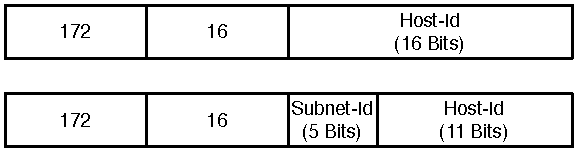
\includegraphics[bb=0bp 0bp 98mm 26mm,clip]{ip/subnet_ex1}

\caption{\label{fig:subnet_ex1}Beispiel einer Subnetzbildung eines Klasse
B Netzes}

\end{figure}


Die Subnetz-Id wird meistens ebenfalls in der dezimalen Form durch
Punkte getrennt angegeben. F�r das Beipiel in Abbildung \ref{fig:subnet_ex1}
lautet die Subnetzmaske 11111111.11111111.11111000.00000000. Das dezimale
�quivalent und damit die Form in der die Subnetzmaske angef�hrt wird
lautet daher 255.255.248.0. Das erste Subnetz wird dann folgenderma�en
angegeben: 172.168.0.0/255.255.248.0. Unter der g�ltigen Voraussetzung,
dass nur zusammenh�ngende Bereiche als Subnetzmaske zugelassen sind,
kann man die Subnetzmaske auch durch Angabe der Anzahl der 1en vom
linken Rand angeben: 172.168.0.0/21. Das n�chste Subnetz hat dann
folgende Adresse: 172.168.8.0/255.255.248.0!

Die bisher behandelte Form von Subnetting wird auch als ,,static
subnetting'' bezeichnet, da alle Teilnetze immer die gleiche Gr��e
haben. Dies ist jedoch oft ung�nstig! Betrachten wir folgendes Beispiel:
Eine Organisation bekommt das Klasse C Netzwerk 193.170.149.0 zugeordnet.
Nehmen wir weiters an, dass aus organisatorischen und technischen
Gr�nden der Bedarf an folgenden Netzen besteht: 4 Netze mit je 10
Hosts, 1 Netz mit 50 Hosts und ein Netz mit 100 Hosts. In Summe ergibt
das 100 Hosts. Insgesamt stehen bei einem Klasse C Netz 254 IP Adressen
f�r Hosts zur Verf�gung. Allerdings ergibt sich folgendes Problem:
es werden insgesamt 6 Teilnetze ben�tigt. Also muss die Subnet-ID
die L�nge 3 haben. Das wiederum bedeutet, dass insgesamt 5 Bits f�r
die Hosts je Teilnetz zur Verf�gung stehen. Das ergibt eine maximale
Anzahl an Hosts von 30 je Teilnetz. Man sieht, dass eine Einteilung
in Teilnetze nicht m�glich ist. Die L�sung daf�r liegt in VLSM (siehe
Abschnitt \vref{sec:VLSM}).

Damit Subnetze eingef�hrt werden k�nnen, m�ssen die Router innerhalb
der Organisation beim Weiterleiten der Pakete (siehe Abschnitt \vref{sec:ip_forwarding})
und auch die Routingprotokolle (wenn nicht statisches Routing verwendet
wird, siehe Abschnitt \vref{sec:routing_protocols}) angepasst werden.


\subsection{VLSM\label{sec:VLSM}}

Um unterschiedlich gro�e Teilnetze einrichten zu k�nnen, wurde VLSM
(variable length subnet masking) eingef�hrt. Darunter versteht man
das Prinzip, dass Subnetze weiter unterteilt werden. Jedes Subnetz
hat seine eigene Subnetzmaske.

Gehen wir wieder von dem Beispiel aus dem vorhergehenden Abschnitt
aus: Eine Organisation bekommt das Klasse C Netz 193.170.149.0 zugeordnet
und ben�tigt 4 Netze je 10 Hosts, 1 Netz mit 50 Hosts und ein Netz
mit 100 Hosts. Die resultierende Aufteilung in entsprechende Subnetze
ist in Abbildung \vref{fig:subnet_ex2} zu sehen. In dieser Abbildung
ist jeweils die Subnetznummer und die Subnetzmaske angegeben.

%
\begin{figure}
\centering

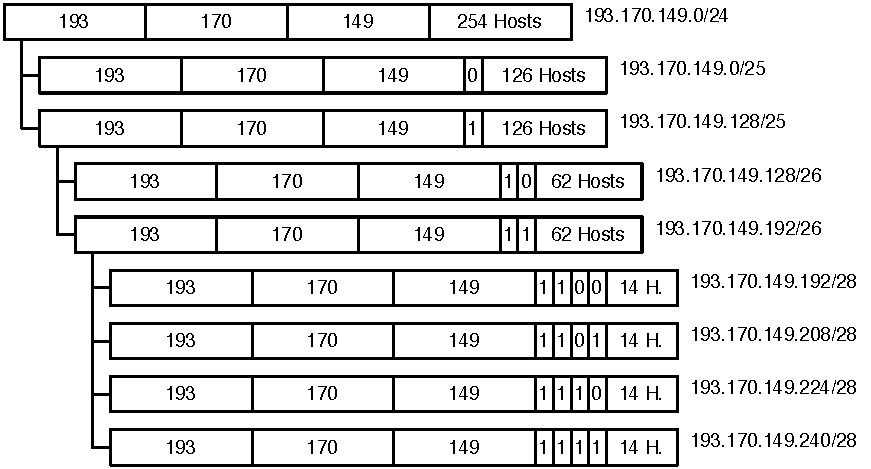
\includegraphics[bb=0bp 0bp 146mm 80mm,clip]{ip/subnet_ex2}

\caption{\label{fig:subnet_ex2}Beispiel f�r Anwendung von VLSM}

\end{figure}



\subsection{Weiterleiten\label{sec:ip_forwarding}}

Weiterleiten in IP funktioniert im Prinzip wie in Abschnitt \vref{sec:forwarding}
beschrieben. In IP kommt es durch die Verwendung von Subnetzmasken
es zu folgendem prinzipiellen Ablauf im Router:
\begin{enumerate}
\item Wenn es sich um das Zielsystem handelt, dann stopp. D.h. der Router
ist das Ziel.
\item F�r jeden Eintrag (Subnetznummer, Subnetmaske, N�chster Hop) der Weiterleitungstabelle

\begin{enumerate}
\item D1 = Zieladresse \& Subnetmaske
\item Wenn D1 == Subnetznummer

\begin{enumerate}
\item dann: Wenn N�chster Hop ist ein Interface

\begin{enumerate}
\item dann: Paket an diesem Interface ausliefern
\item anderenfalls: Paket an dem Interface ausliefern, das zu diesem Router
f�hrt
\end{enumerate}
\end{enumerate}
\end{enumerate}
\item Wenn kein Router gefunden, dann an den Default-Router weitersenden.
Ist kein Defaultrouter definiert, dann ICMP Fehlernachricht ,,network
unreachable'' schicken (siehe Abschnitt \vref{sec:ICMP}).
\end{enumerate}
Es handelt sich hier um den prinzipiellen Ablauf und nicht um eine
Beschreibung einer konkreten Implementierung, da es nicht sehr sinnvoll
ist, jedes Mal eine lineare Suche in der Weiterleitungstabelle durchzuf�hren
bzw. die bitweise UND Verkn�pfung immer neu zu berechnen, auch wenn
sich die Subnetmaske nicht ge�ndert hat.

Der Default Router, an den alle IP Pakete weitergeleitet werden, f�r
die keine Route in der Weiterleitungstabelle eingetragen ist wird
oft auch Default Gateway genannt, obwohl es sich im strengen Sinne
um kein Gateway handelt.


\subsection{CIDR\label{sec:CIDR}}

Der Ersch�pfung der IP Adressen wird durch Subnetting nicht weiter
vorgebeugt, da eine Organisation, die z.B. 2 Adressen ben�tigt, ein
Klasse C Netzwerk zugewiesen bekommt. D.h. die ,,Effizienz'' betr�gt
2/254{*}100\% also 0.78\%! Nehmen wir als weiteres Beispiel an, dass
eine Organisation 256 Hosts an das Internet anschlie�en muss. Es wird
also ein Klasse B Netzwerk ben�tigt. D.h. die ,,Effizienz'' betr�gt
256/65534{*}100\% also lediglich 0.39\%!

Ben�tigt eine Organisation mehr als 254 Adressen aber nicht nahezu
65534 Adressen, dann bekommt sie wahrscheinlich anstatt eines Klasse
B Netzes mehrere Klasse C Netze zugewiesen, da freie B Netze nur in
beschr�nkten Umfang vorhanden sind bzw. die Effizienz der Adressvergabe
verbessert wird. Damit wachsen jedoch automatisch die Routertabellen
im Internet an, wodurch es zu Performanceinbu�en kommt. Ein weiteres
Problem ist, dass Routertabellen nur eine beschr�nkte Gr��e haben.

Trotz der Vorteile des Subnetting, private Netze effizient zu partitionieren,
bleibt die ineffiziente Adressvergabe weiters bestehen. Gel�st werden
diese Probleme mit CIDR (engl. classless inter-domain routing). CIDR
wird auch supernetting genannt, da es sich im Prinzip, um eine analoge
L�sung wie das subnetting handelt, allerdings auf Internet-Ebene.

CIDR versucht die Anzahl der Routingeintr�ge in den Routern des Internet
zu minimieren. Das wird so gemacht, dass eine Organisation mehrere
\emph{aufeinanderfolgende} z.B. Klasse C Adressbereiche zugewiesen
bekommt. Diese aufeinanderfolgenden Routen werden zu einer Route mit
Hilfe einer Netzmaske (meist angegeben durch Suffixdarstellung) aggregiert.

Nehmen wir an, dass eine Organisation einen Bedarf an 16 Klasse C
Netzen hat und diese Organisation deshalb einen zusammenh�ngenden
Bereich von 192.4.16.0/24 bis 192.4.31.0/24 zugewiesen bekommt. Man
erkennt, dass die oberen 20 Bits aller dieser Adressen gleich ist,
n�mlich 11000000 00000100 0001. Das bedeutet, dass dadurch eine 20
Bit lange effektive Netznummer erzeugt worden ist. D.h. das resultierende
Netz l�sst sich als 192.4.16.0/20 angeben. Man sieht, dass die Angabe
in gleicher Weise wie beim Subnetting vorgenommen wird. Das Ergebnis
ist, dass nur mehr ein Routereintrag f�r diese Organisation vorgenommen
werden muss.

Dieses Verfahren l�sst sich auch �ber mehrere Organisationen kaskadieren:
Werden die Adressbereiche mehrerer Organisationen ebenfalls aufeinanderfolgend
vergeben, k�nnen diese Adressbereiche ebenfalls zu einem Eintrag aggregiert
werden! Damit sinkt die Anzahl der Routereintr�ge weiter.

Damit wird mit CIDR sowohl die Effizienz der Vergabe verbessert als
auch die Anzahl der Routereintr�ge minimiert.

�hnlich wie bei Subnetting m�ssen die Routingprotokolle (siehe Abschnitt
\vref{sec:routing_protocols}) ebenfalls mit dieser Form der Adressangabe
umgehen k�nnen.


\section{Aufbau eines Datagram}

Der Aufbau eines IPv4 Datagram ist in Abbildung \vref{fig:ip_datagram}
zu sehen.

%
\begin{figure}
\centering

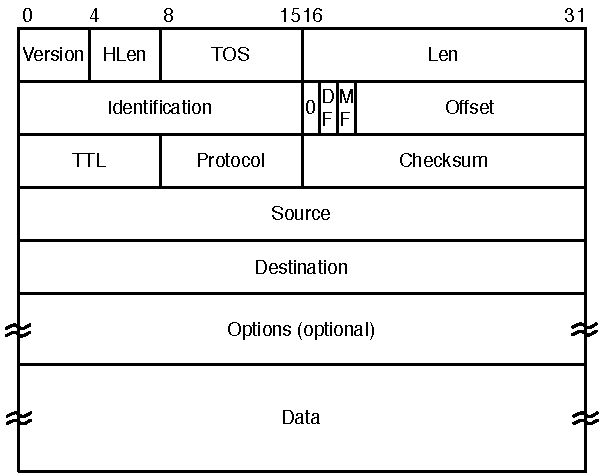
\includegraphics[bb=0bp 0bp 102mm 80mm,clip]{ip/ip-datagram}

\caption{\label{fig:ip_datagram}IP Datagram}

\end{figure}

\begin{labeling}{00.00.0000}
\item [{Version}] Enth�lt entweder den Wert 4 f�r IPv4 oder den Wert 6
f�r IPv6. An Hand dieser 4 Bits kann jede Implementierung des TCP/IP
Protokollstacks sofort erkennen, um welches IP Paket es sich handelt.
Das ist deshalb wichtig, da der Aufbau eines IPv6 Datagrams ansonsten
verschieden ist!
\item [{HLen}] Gibt die Anzahl der 32 Bitworte an, die ein Header inklusive
Optionen lang ist. Der Optionenbereich ist variabel, daher ist das
Feld HLen notwendig.
\item [{TOS}] Type-of-service Feld wurde schon f�r mehrere Funktionen eingesetzt.
Seit 1998 wird es lt. RFC 2474 f�r DS (differential services) verwendet.
DS ist ein bestimmtes Quality of Service (QoS) Verfahren zur Priorisierung
von IP Paketen.
\item [{Len}] Gibt die Gesamtl�nge eines IP Datagrams in Byte an. Da hierf�r
16 Bit zur Verf�gung stehen, ist die maximale Gr��e eine IP Datagrams
auf 65535 Bytes beschr�nkt.
\item [{Identification}] Das Feld Identification wird im Zuge der Fragmentierung
verwendet und stellt eine eindeutige Identifikation zur Verf�gung
(siehe Abschnitt \vref{sec:fragmenting}).
\item [{Flags}] Zwischen Identifcation und Offset sind 3 Flags untergebracht:

\begin{labeling}{00.00.0000}
\item [{0}] Das erste Bit muss immer ein 0 Bit sein.
\item [{DF}] ,,Do not fragment'' wird ebenfalls im Zuge der Fragmentierung
verwendet (siehe Abschnitt \vref{sec:fragmenting}).
\item [{MF}] ,,More fragments'' wird ebenfalls im Zuge der Fragmentierung
verwendet (siehe Abschnitt \vref{sec:fragmenting}).
\end{labeling}
\item [{Offset}] Offset wird ebenfalls im Zuge der Fragmentierung verwendet
(siehe Abschnitt \vref{sec:fragmenting}).
\item [{TTL}] ,,Time-to-live'' gibt die Lebensdauer des Paketes an und
wird zur Verhinderung endlos kreisender Pakete eingesetzt. Der sendende
Host setzt TTL auf einen Anfangswert und jede Station, die das Datagram
weiterreicht vermindert den Z�hler um eins. Hat TTL den Wert 0 erreicht,
dann wird das Paket verworfen. �blich sind die Anfangswerte von 64
und 128.
\item [{Protocol}] Dieses Feld enth�lt eine eindeutige Zahl, die das verwendete
Transportprotokoll angibt. Diese Nummern werden von der IANA (Internet
Assigned Numbers Authority) verwaltet. Beispiele: 1 (ICMP), 6 (TCP),
17 (UDP).
\item [{Checksum}] Das ist eine Pr�fsumme �ber den gesamten Header. Die
Idee ist, dass die Korrektheit der Daten von einem �bergeordneten
Protokoll �berpr�ft werden muss und dadurch die Berechnung der Pr�fsumme
schnell durchgef�hrt werden kann, sodass die Verz�gerung bei der Weiterleitung
in einem Router gering gehalten werden kann. Das Verfahren der Berechnung
der Checksumme ist in Abschnitt \vref{sec:error_detection_checksums}
beschrieben.
\item [{Source}] Die IP-Adresse des Senders.
\item [{Destination}] Die IP-Adresse des Empf�ngers.
\item [{Options}] Das Options-Feld ist daf�r gedacht zus�tzliche variable
Informationen mitzu�bertragen, f�r die es nicht notwendig ist einen
festen Platz in der Header-Struktur vorzusehen. Es handelt sich hierbei
um Informationen zum Routing, Security, Zeitstempel,\ldots{} Eventuell
muss mit Nullen aufgef�llt werden, damit der Header an einer 32 Bitgrenze
endet.
\end{labeling}

\section{Fragmentierung\label{sec:fragmenting}}

Die Anpassung der Paketl�nge an eine kleinere maximale Paketgr��e
der untenliegenden Schicht, also die Segmentierung (siehe Abschnitt
\vref{sec:segmenting}), wird in IP Fragmentierung genannt. Wie im
Abschnitt \vref{sec:ethernet_frame} beschrieben besteht ein Datenblock
in einem Ethernet Frame aus maximal 1500 Bytes w�hrend ein Paket in
einem FDDI Netzwerk maximal 4500 Bytes beinhalten kann. Wird ein IP
Paket �ber mehrere Netze mit unterschiedlichen Technologien versendet,
besteht entweder die M�glichkeit sicherzustellen, dass die IP Pakete
maximal die kleinste Gr��e aller Technologien annehmen, oder die Pakete
jeweils an die verschiedenen Technologien durch Segmentierung und
Reassemblierung anzupassen.

IPv4 unterst�tzt den Ansatz mittels Segmentierung und Reassemblierung.
Das zentrale Konzept ist, dass es bei jeder Technologie eine maximale
�bertragungseinheit (engl. max transmission unit oder MTU) gibt, die
die maximale Paketgr��e angibt, die �ber ein Netz �bertragen werden
kann. Im Fall von Ethernet betr�gt dieser Wert 1500. In IP m�ssen
die Router bzw. die physische Netztechnologien eine minimale MTU von
zumindest 576 Bytes unterst�tzen.

Das Header-Feld DF zeigt an, dass dieses IP Paket nicht fragmentiert
werden darf. Kommt ein IP Paket zu einen Router oder einem Netz, das
eine Fragmentierung dieses Paketes erfordern w�rde, dann wird eine
ICMP Nachricht (siehe \vref{sec:ICMP}) vom Typ 3 mit Code 5 (Fragmentation
needed but the Do Not Fragment bit was set) gesendet.

Das Zusammenspiel der Identification, des Flags MF und des Offsets
ist in folgenden Beispielen zu sehen, wenn wir von einer L�nge der
zu �bertragenden Daten von 1400 ausgehen:
\begin{itemize}
\item nicht fragmentiertes Paket mit: Identification = x; MF = 0; Offset
= 0; Data (1400 Bytes)
\item fragmentierte Pakete bei einer MTU mit 532 Bytes mit:

\begin{enumerate}
\item Identification = x; MF = 1; Offset = 0; Data (512 Bytes)
\item Identification = x; MF = 1; Offset = 64; Data (512 Bytes)
\item Identification = x; MF = 0; Offset = 128; Data (376 Bytes)
\end{enumerate}
\end{itemize}
Das Prinzip der Fragmentierung ist folgendes:
\begin{itemize}
\item Das Identifikationsfeld bezeichnet ein IP Datagram, wird vom Sender
frei gew�hlt und ist f�r alle Fragmente gleich.
\item Das Flag MF ist gesetzt, wenn weitere Fragmente folgen.
\item Der Offset gibt den Offset des Fragmentes relativ zum gesamten Datenblock
in jeweils 8 Byte an (512 / 8 = 64). Die Einheit von 8 Bytes liegt
darin begr�ndet, das nur 13 Bits f�r den Offset zur Verf�gung stehen
und die maximale Gr��e eine IP Datagrams 65535 Bytes ist.
\item Das Datenfeld beinhaltet 512 Bytes, da 20 Bytes f�r den IP Header
anfallen.
\item Die Fragmente werden vom Empf�nger im Zuge der Reassemblierung wieder
zusammengesetzt. Der Empf�nger kann dies deshalb durchf�hren, da er
alle zusammengeh�rigen Fragmente an der gleichen Identifikation erkennt.
Geht eines der Fragmente verloren, dann wird das gesamte IP Datagram
samt allen bisher empfangenen Fragmente verworfen. D.h. IP versucht
nicht, fehlende Fragmente wieder zu beschaffen. Die Reassemblierung
erfolgt am empfangenden Host und nicht an einem Router.
\end{itemize}

\section{ICMP\label{sec:ICMP}}

ICMP (engl. internet control message protocol) ist ein Hilfsprotokoll,
dessen Funktion prim�r die Unterst�tzung des verbindungslosen und
nicht fehlergesicherten IP mit zus�tzlichen Status-, Steuer- und Fehlerinformationsmeldungen
ist. Neben IP k�nnen auch h�her geschichtete Protokoll wie TCP, Routingprotokolle
oder auch Anwendungen die Information von ICMP Nachrichten auswerten.

Die bekannteste Anwendung von ICMP ist die Verwendung der ICMP Echo
Request bzw. der ICMP Echo Reply Nachricht, die in der ping Anwendung
eingesetzt wird.

Jede ICMP Nachricht besteht aus einem Typ und einem Code, einer Pr�fsumme
und einem Inhalt, der von Typ und Code abh�ngig ist. Jede dieser Nachrichten
ist entweder eine Query Nachricht oder eine Fehler Nachricht.

Beispielhaft sind die wichtigsten ICMP Nachrichtentypen angef�hrt:
\begin{itemize}
\item Echo Request (Typ 8, Code 0) und Echo Reply (Typ 0, Code 0). Query-Nachricht.
\item Ziel nicht erreichbar (Typ 3, Code 0-15). Fehler-Nachricht. Dieser
Nachrichtentyp inkludiert die Fehlernachrichten f�r ,,Netzwerk nicht
erreichbar'', ,,Host nicht erreichbar'', ,,Protokoll nicht erreichbar'',
,,Port nicht erreichbar'', ,,Fragmentierung erforderlich, aber
DF Bit gesetzt'', ,,Source Route fehlerhaft'', ,,Zielnetzwerk
unbekannt'',...
\item Quelle unterdr�cken (engl. source quench) (Typ 4, Code 0). Fehler-Nachricht.
Dieser Nachrichtentyp stellt die einzige M�glichkeit von IP dar, einem
Sender mitzuteilen, dass er seine Datenrate reduzieren soll. Der Empf�nger
sendet so lange solche Nachrichten an den Sender solange dieser die
Datenrate reduzieren soll. Empf�ngt der Sender keine weiteren ICMP
Nachrichten, dann kann er seine Datenrate wieder erh�hen. D.h. in
dieser Nachricht gibt es keine explizite M�glichkeit die Datenrate
anzugeben bzw. anzugeben wann wieder eine h�here Datenrate erlaubt
ist. Es ist im Standard explizit festgehalten, dass im Falle eines
Verwerfens eines IP-Datagrams ein ICMP source quench Nachricht gesendet
werden kann (aber nicht muss). Auf jeden Fall muss der Empfang eines
solchen ICMP Paketes an die Transportschicht weitergegeben werden.
Im Falle von TCP sollte TCP die Senderate reduzieren und im Falle
von UDP sollte die Anwendung darauf entsprechend reagieren.
\item Redirect (Typ 5, Code 0-3). Fehler-Nachricht. Dient der Signalisierung
eines Routers an einen Sender, dass ein besserer Router f�r die eingegangenen
Pakete existiert. Diese stellen ein Sicherheitsrisiko, da gef�lschte
ICMP Pakete den Sender veranlassen seine Paket an einen anderen Router
zu senden.
\item Router-Advertisement (Typ 9, Code 0) und Router-Anforderung (Typ 10,
Code 0).  Dienen dazu, um Router in einem lokalen Netzwerk zu erkennen
(Sicherheitsrisiko).
\end{itemize}

\section{ARP\label{sec:ARP}}

Mittels Weiterleiten kommt ein IP Datagram zum richtigen Netz. Die
offene Frage ist jetzt, wie das Paket zum richtigen Host kommt. Jedes
Ger�t ist mit seiner MAC Adresse eindeutig zu adressieren. Es ist
notwendig die MAC Adresse zu kennen, um einen Host in einem Segment
zu adressieren.

ARP (engl. address resolution protocol) ist ein Protokoll, das die
MAC Adresse eines Hosts ermittelt. Dazu macht es sich die Eigenschaft
zu Nutze, dass Ethernet und andere LAN Technologien ebenfalls �ber
eine Broadcast Eigenschaft verf�gen. Jeder Host merkt sich alle ihm
schon bekannten Zuordnungen von IP Adresse zu MAC Adresse in einem
Cache (ARP Cache oder ARP Tabelle genannt). Soll ein Paket einem Host
in einem Netz zugestellt werden, dann wird zuerst dieser Cache konsultiert.
Ist eine Zuordnung dort vorhanden, dann wird sie verwendet, um das
Paket zuzustellen. Ist keine Zuordnung f�r diese IP Adresse im Cache
vorhanden, dann wird ein Broadcast Frame an alle Hosts in diesem Segment
gesendet, der die fragliche IP Adresse enth�lt. Der gesuchte Host
antwortet mit seiner IP Adresse, worauf dem ARP Cache die neue Zuordnung
hinzugef�gt werden kann.

Diejenigen Stationen, die ebenfalls den Broadcast empfangen, k�nnen
diese Zuordnung (Sender IP, Sender MAC) ebenfalls lernen. Ist so eine
Zuordnung schon im ARP Cache enthalten wird sie lediglich aufgefrischt
und der Timer zur�ckgesetzt. L�uft der Timer ab, dann wird die Zuordnung
aus dem Cache gel�scht.

ARP wurde nicht unter dem Gesichtspunkt der Sicherheit entworfen und
ist deshalb besonders anf�llig: Unter ARP-Spoofing versteht man das
gezielte Versenden gef�lschter ARP Pakete, die dazu benutzt werden,
den Datenverkehr zwischen zwei Hosts in einem Netz abzuh�ren oder
zu manipulieren.

RARP (engl. reverse address resolution protocol) ist ein Protokoll,
das die inverese Funktionalit�t aufweist und die IP Adressse zu einer
MAC Adresse finden soll. Es wird allerdings nicht mehr eingesetzt,
da es durch BOOTP und in weiterer Folge von DHCP abgel�st worden ist.
Die Gr�nde liegen darin, dass man mittels RARP nur die IP Adresse,
aber keine zus�tzlichen Informationen wie z.B. die Netzmaske oder
den Default-Router ermitteln kann.



\chapter{Transportprotokolle TCP und UDP\label{sec:tcpudp}}


\section{Adressierung}

Die Adresserierung in IP wird �ber die IP Adressen vorgenommen, die
global eindeutig sein m�ssen. Auf der Transportebene wird eine weitere
Form der Adressierung ben�tigt, da es sich um eine Ende-zu-Ende Kommunikation
auf Prozessebene handelt. Das bedeutet, dass �ber die Transportschicht
direkt zwei Prozesse miteinander verbunden sind und miteinander kommunizieren.

In diesem Sinne muss es eine M�glichkeit geben, einen Prozess auf
einem Host zu identifizieren. Das Konzept, das TCP/IP auf dieser Ebene
eingef�hrt hat sind die Ports. Es handelt sich dabei um einen nummerischen
Bezeichner, der Werte im Bereich von 0 bis 65535 annehmen kann.

In diesem Zusammenhang f�hrt TCP das Konzept eines Kommunikationsendpunktes
ein, der als ,,socket'' bezeichnet wird und sich aus der IP Adresse
und dem Port zusammensetzt. Zwei Sockets, n�mlich der Sender-Socket
und der Empf�nger-Socket identifizieren gemeinsam mit der Angabe des
verwendeten Transportprotokolls eindeutig eine Kommunikation in Internet!
Ein lokaler Socket kann gleichzeitig in mehreren Kommunikationsverbindungen
verwendet werden.

F�r jede Nachricht, die von einem Senderprozess (also eine laufende
Anwendung) an einen Empf�ngerprozess (ebenfalls eine laufende Anwendung)
gesendet wird, gibt es einen Sender-Socket und einen Empf�nger-Socket.
In der Regel ist es so, dass ein Prozess an einem Empf�nger-Socket
lauscht und Nachrichten an diesem empfangen kann. Der Senderprozess
schickt eine Nachricht mittels eines Sender-Socket unter Angabe des
Transportprotokolls �ber den Empf�nger-Socket an den Empf�ngerprozess.
Dieser Empfangsprozess erbringt in der Regel einen Dienst und wird
auf die eingegangenen Nachrichten mittels Antworten reagieren.

Dieses Senden der Nachrichten verwendet das unterliegende IP. Der
Sendeprozess �bergibt die Nachricht an die Transportschicht. Die Transportschicht
packt die Nachricht in ein TCP oder UDP Paket und reicht dieses an
IP weiter. Beim Empf�nger werden die Pakete wieder entpackt und an
den richtigen Prozess weitergegeben. Dies wird, analog zu den Signalen,
als Multiplexing bzw. Demultiplexing bezeichnet. Die zentrale Information,
die zum Multiplexen bzw. Demultiplexen verwendet wird sind die Ports.

Portnummern von 0 bis 1023 werden als sogenannte ,,well known ports''
bezeichnet und von der IANA verwaltet und f�r Anwendungen reserviert.
Unter Unix werden diese Ports insoferne speziell behandelt als das
ein passives �ffnen (siehe \vref{sec:tcp_fsm}) nur Prozessen mit
der Benutzernummer 0 erlaubt wird. Bestimmte Ports sind bestimmten
Diensten zugeordnet, wichtige Dienste sind:

\begin{tabular}{|c|c|c|l|}
\hline 
Port\# & Protokoll & Schl�sselwort & Beschreibung\tabularnewline
\hline
\hline 
20 & tcp & ftp-data & file transfer protocol (Datenkanal)\tabularnewline
\hline 
21 & tcp & ftp & file transfer protocol (Steuerkanal)\tabularnewline
\hline 
22 & tcp & ssh & secure socket shell\tabularnewline
\hline 
25 & tcp & smtp & simple mail transfer protocol\tabularnewline
\hline 
53 & tcp+udp & domain & domain name system\tabularnewline
\hline 
67 & udp & dhcp & dynamic host configuration protocol (server)\tabularnewline
\hline 
68 & udp & dhcp & dynamic host configuration protocol (server)\tabularnewline
\hline 
80 & tcp & http & hyper text transfer protocol\tabularnewline
\hline 
110 & tcp & pop & post office protocol\tabularnewline
\hline 
113 & tcp & ident & ident protocol\tabularnewline
\hline 
119 & tcp & nntp & network news transfer protocol\tabularnewline
\hline 
123 & tcp & ntp & network time protocol\tabularnewline
\hline 
143 & tcp & imap & internet mail access protocol\tabularnewline
\hline 
161 & udp & snmp & simple network management protocol\tabularnewline
\hline 
389 & tcp & ldap & lightweight directory access protocol\tabularnewline
\hline 
443 & tcp & https & http over SSL\tabularnewline
\hline 
514 & tcp & syslog & syslog\tabularnewline
\hline
\end{tabular}


\section{UDP\label{sec:udp}}

UDP (engl. user datagram protocol) ist das einfachere Transportprotokoll,
das TCP/IP zur Verf�gung stellt. Es wurde 1980 im RFC 768 publiziert
und seit dem nicht ver�ndert.

Das Entwurfsziel war ein verbindungsloses, unzuverl�ssiges Ende-zu-Ende
Transportprotokoll zur Verf�gung zu stellen, das einfach ist und eine
schnelle Kommunikation erlaubt. Es ist charakterisiert durch folgende
Eigenschaften:
\begin{itemize}
\item Es ist unzuverl�ssig: Es gibt keine Garantie ob Daten angekommen sind,
es wird nicht erkannt, ob Daten verloren gegangen sind und es gibt
keine Garantie, dass die Daten in der Reihenfolge ankommen, in der
sie abgesendet worden sind.
\item Es gibt keinen Mechanismus zur Flusskontrolle.
\item Es erfolgt eine einfache �berpr�fung auf die Korrektheit der �bertragenen
Daten
\end{itemize}
Man sieht, dass UDP an sich nur zwei zus�tzliche Eigenschaften gegen�ber
IP zur Verf�gung stellt: Multiplexing/Demultiplexing und �berpr�fung
auf Korrektheit der Daten.

UDP eignet sich gut f�r Audio- und Videostreams und au�erdem wird
es auch bei einigen wichtigen Protokollen, wie DNS, SNMP und DHCP
eingesetzt.


\subsection{Aufbau eines Datagrams}

Der Aufbau eines UDP Datagram ist in Abbildung \vref{fig:udp_datagram}
zu sehen.

%
\begin{figure}
\centering

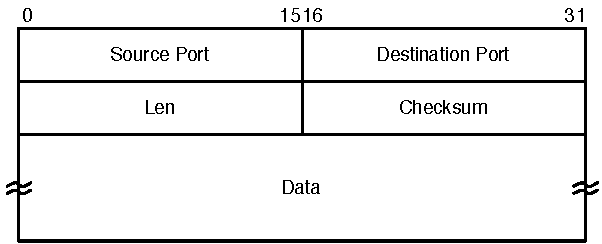
\includegraphics[bb=0bp 0bp 102mm 40mm,clip]{tcpudp/udp-datagram}

\caption{\label{fig:udp_datagram}Aufbau eine UDP Datagrams}

\end{figure}

\begin{labeling}{00.00.0000}
\item [{Source~Port}] 0--65535
\item [{Destination~Port}] 0--65535
\item [{Len}] L�nge des vollst�ndigen UDP Datagrams inklusive Header und
Datenfeld in Bytes. D.h. der minimale Wert ist 8. Man beachte, dass
es sich hierbei um eine redundante Information handelt, da im Feld
Len von IP ebenfalls die L�nge des Datenbereichs angegeben ist.
\item [{Checksum}] Pr�fsumme. Der Algorithmus funktioniert wie derjenige
zur Berechnung der Pr�fsumme in IP, jedoch wird als Grundlage der
Header des UDP Datagrams, das Datenfeld des UDP Datagrams und ein
sogenannter Pseudoheader herangezogen, der sich folgenderma�en zusammensetzt:
IP Quelladresse (32 Bits), IP Zieladresse (32 Bits), der Wert 0 (8
Bits) das Feld Protocol vom IP Header (8 Bits) und das Feld Len vom
UDP Header (16 Bits). Der Pseudoheader wird nicht �bertragen: er wird
nur zur Berechnung der Pr�fsumme herangezogen!\\
Man sieht, dass im Gegensatz zu IP auch das Datenfeld bei der Berechnung
der Pr�fsumme herangezogen wird.
\item [{Data}] Datenfeld
\end{labeling}
Dass UDP die Pr�fsumme ebenfalls �ber das Datenfeld berechnet ist
einerseits ein Vorteil, aber auch andererseits unter Umst�nden ein
Nachteil, wenn der Overhead durch die Berechnung (z.B. bei Datenraten
gr��er als 1 GBit/s) zu gro� ausf�llt. 


\section{TCP\label{sec:tcp}}

TCP (engl. transmission control protocol) ist das komplexere Transportprotokoll,
das TCP/IP zur Verf�gung stellt. Es wurde 1981 im RFC 793 publiziert
und seit dem nicht ver�ndert. Erweiterungen sind in zus�tzlichen RFCs
spezifiziert.

Das Entwurfsziel war ein verbindungsorientiertes, zuverl�ssiges Ende-zu-Ende
Transportprotokoll zur Verf�gung zu stellen, das einfach ist und eine
schnelle Kommunikation erlaubt. Es ist charakterisiert durch folgende
Eigenschaften:
\begin{itemize}
\item Es ist zuverl�ssig: verloren gegangene oder falsche Daten werden wieder
neu �bermittelt, doppelt ankommende Daten werden verworfen und es
wird sichergestellt, dass die Daten in der Reihenfolge des Absendens
dem Empf�ngerprozess weitergereicht werden.
\item Verbindungen werden unterst�tzt und verwaltet: Verbindungsauf- und
Abbau.
\item Die Daten�bertragung ist vollduplex: es werden gleichzeitig zwei Datenstr�me
(einer in jeder Richtung) unterst�tzt.
\item Zur Daten�bertragung wird eine Abstraktion �ber Streams zur Verf�gung
gestellt. D.h. die Anwendungsschicht kann einen Byte-Strom zu TCP
senden bzw. einen Byte-Strom von TCP lesen. Dazu stellt TCP eine Art
von Segmentierung zur Verf�gung (siehe Abschnitt \vref{sec:tcp_segment}
und \vref{sec:tcp_segmenting}).
\item Es gibt einen Mechanismus zur Flusskontrolle. Flusskontrolle hindert
den Sender daran, die Kapazit�t des Empf�ngers zu �berschreiten. Es
handelt sich also um einen Mechanismus auf der Ende-zu-Ende Ebene
und betrifft die beiden kommunizierenden Hosts.
\item Es gibt eine �berlastkontrolle. �berlastkontrolle bietet einen Schutz
vor �berlastung des Netzes. Es handelt sich um einen Mechanismus der
einerseits den Sender und andererseits das Netz betrifft.
\item Es erfolgt eine einfache �berpr�fung auf Korrektheit der �bertragenen
Daten.
\item Es ist als robustes Protokoll entworfen und folgt dem Grundsatz: konservativ
in dem was gesendet wird und tolerant bzgl. der empfangenen Segmente.
\end{itemize}

\subsection{Aufbau eines Segmentes\label{sec:tcp_segment}}

Bei TCP werden die einzelnen Pakete als Segmente genannt. Der Aufbau
eines TCP Segmentes ist in Abbildung \vref{fig:tcp_segment} zu sehen.

%
\begin{figure}
\centering

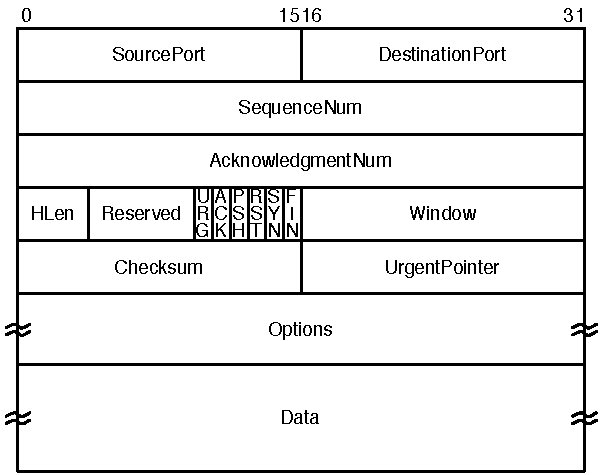
\includegraphics[bb=0bp 0bp 102mm 79mm,clip]{tcpudp/tcp-segment}

\caption{\label{fig:tcp_segment}Aufbau eine TCP Segmentes}

\end{figure}

\begin{labeling}{00.00.0000}
\item [{SourcePort}] 0--65535
\item [{DestinationPort}] 0--65535
\item [{SequenceNum}] Die Sequenznummer wird f�r den Window Sliding Mechanismus
verwendet. Da TCP ein byte-orientiertes Protokoll ist, hat jedes Byte
eine Sequenznummer. Dieses Feld enth�lt die Sequenznummer des ersten
Byte im Datenfeld.
\item [{AcknowledgmentNum}] Wird dem Sender ein Segment gesendet, das das
ACK Bit gesetzt hat, dann enth�lt dieses Feld die Best�tigungsnummer.
Sie gibt die Nummer der n�chsten erwarteten Sequenznummer an. Alle
Bytes mit einer kleineren Best�tigungsnummer werden hiermit best�tigt.
\item [{HLen}] 4 Bit: L�nge des Headers in 32 Bitworten bis zum Beginn
des Datenfeldes.
\item [{Reserved}] 6 Bit langes Bitfeld, das lauter 0en enthalten muss.
\item [{URG}] Das Bit URG (urgent) zeigt der empfangenen Anwendung an,
dass Daten priorisiert behandelt werden sollen. Die dringenden Daten
befinden sich am Anfang des Datenbereiches und reichen bis zu der
Stelle, die durch das Feld UrgentPtr angezeigt werden, das auf das
letzte Oktett der dringlichen Daten zeigt. URG wird selten verwendet,
z.B. bei telnet oder rlogin. Diese Kennzeichnung ist deshalb notwendig,
da TCP den Inhalt der Daten nicht kennt; f�r TCP handelt es sich um
einen Strom von Daten, die auf Grund der Stream-Eigenschaft mittels
des FIFO Prinzips �bertragen werden.\\
�bertr�gt man z.B. eine gro�e Datei und will diesen Transfer der
Daten abbrechen, dann ist es nicht sinnvoll ein Abbruch-Kommando am
Ende des Datei hinten anzuf�gen. Es muss eine M�glichkeit geben das
Abbruch-Kommando vorzureihen. TCP stellt eine M�glichkeit zur Verf�gung
solche dringenden Daten zu versenden. Es werden diese Daten am Anfang
des Datenbereiches eines Segmentes platziert, das URG Flag gesetzt
und der UrgentPtr richtig gesetzt. Beim Empf�nger werden diese Daten
vorgereiht und dem Prozess vorrangig und als ,,urgent'' markiert
ausgeliefert. Die restlichen Daten des Datenbereiches werden normal
im Datenstream ausgeliefert.
\item [{ACK}] Mittels ACK (acknowledgement) best�tigt TCP den Erhalt von
Daten (siehe Acknowledgment Number).
\item [{PSH}] Ist PSH (push) gesetzt, dann soll der TCP/IP Stack dieses
Segment ohne weiteres Zwischenspeichern an die Anwendung weiterreichen.
Daf�r bietet TCP eine push Funktion an, die von der Anwendungsschicht
aufgerufen werden kann. D.h. die normale Pufferung der Bytes bis sich
gen�gend Bytes angesammelt haben, wird ausgeschalten, das PSH Flag
gesetzt und alle Daten werden sofort abgesendet. Auf der Empf�ngerseite
wird erkannt, dass das PSH Flag gesetzt ist und die Daten werden sofort
an die Anwendung weitergereicht. D.h. auch hier wird nicht gewartet
bis ,,gen�gend'' Daten eingetroffen sind.
\item [{RST}] Dieses Bit RST (reset) wird verwendet, um eine sofortige
Aufl�sung der TCP Verbindung anzuzeigen und sollte nicht der normale
Vorgang zum Beenden einer Verbindung sein. Es wird z.B. verwendet,
wenn der Empf�nger ein unerwartetes Segment erhalten hat, wodurch
ein Fehlerzustand eingetreten ist und dadurch die Verbindung abgebrochen
werden muss.
\item [{SYN}] Beim Verbindungsaufbau wird SYN (synchronize) verwendet (siehe
\vref{sec:connection_management}).
\item [{FIN}] Beim Verbindungsabbau wird FIN (finish) verwendet (siehe
\vref{sec:connection_management}).
\item [{Window}] Dieses Feld gibt die Fenstergr��e an. Gemeinsam mit SequenceNum,
AcknowledgeNum wird der Sliding Window Mechanismus in TCP realisiert
(siehe Abschnitt \vref{sec:tcp_sliding_window}).
\item [{Checksum}] Pr�fsumme. Der Algorithmus funktioniert wie derjenige
zur Berechnung der Pr�fsumme in IP, jedoch wird als Grundlage der
Header des TCP Segmentes, das Datenfeld des TCP Segmentes und ein
sogenannter Pseudoheader herangezogen, der sich folgenderma�en zusammensetzt:
IP Quelladresse (32 Bits), IP Zieladresse (32 Bits), der leere Checksum-Wert
0 (8 Bits) das Feld Protocol vom IP Header (8 Bits) und das Feld Len
vom TCP Header (16 Bits). Der Pseudoheader wird nicht �bertragen:
er wird nur zur Berechnung der Pr�fsumme herangezogen!\\
Man sieht wiederum, dass im Gegensatz zu IP auch das Datenfeld
bei der Berechnung der Pr�fsumme herangezogen wird.
\item [{UrgentPtr}] Bei dem Feld UrgentPtr handelt es sich um einen Zeiger
auf das letzte Oktett der dringlichen Daten und wird nur interpretiert,
wenn das URG Flag gesetzt ist.
\item [{Options}] Das Feld Options kann mehrere Optionen beinhalten. Jede
Option besteht aus einem Feld ,,Art der Option'' (option-kind) und
eventuell einem Feld ,,L�nge der Option'' (option-length) gefolgt
von einem Feld ,,Daten der Option'' (option-data). Einige Optionen
haben keine Daten und damit auch kein L�ngenfeld. In RFC 793 sind
nur 3 Optionen definiert:

\begin{itemize}
\item ,,End of Option List'' (option-kind=0) kennzeichnet das Ende der
Optionen und wird nur verwendet, wenn das Ende der Optionen nicht
mit dem Ende des TCP Headers �bereinstimmt.
\item ,,No-Operation'' (option-kind=1) kann verwendet werden, um Optionen
von einander zu trennen und wird eingesetzt, wenn der Sender Optionen
an Wortgrenzen beginnen lassen will.
\item ,,Maximum Segment Size (MSS)'' (option-kind=2, option-length=4,
option-data enth�lt MSS). Bzgl. MSS siehe Abschnitt \vref{sec:tcp_segmenting}.
Diese Option kann nur in einem Segment vorhanden sein, das das SYN
Bit gesetzt hat.
\end{itemize}
Nach dem Ende der Optionen muss der verbleibende Platz zur n�chsten
32 Bit Grenze mit Nullen aufgef�llt (engl. padding) werden. Weitere
Optionen wurden in getrennten RFCs definiert.

\item [{Data}] Datenfeld. Betrachtet man die maximale MTU bei Ethernet-Netzen
sieht man folgendes: der minimale TCP Header ist 20 Bytes und damit
entsteht gemeinsam mit dem IP Header eine minimale Headerl�nge von
40 Bytes. Da die maximale Gr��e des Datenbereiches eines Ethernet-Frames
bei 1500 Bytes liegt, kommt man auf eine max. Datengr��e bei TCP auf
1460 Bytes.
\end{labeling}

\subsection{Verbindungsauf- und Abbau\label{sec:connection_management}}


\subsubsection{Verbindungsaufbau}

Der Verbindungsaufbau wird in TCP mittels eines 3-Wege-Handshake (engl.
three-way handshake) vorgenommen und wird durch die Synchronisierung
zweier Sequenznummern (eine am Server, eine am Client) erreicht:
\begin{enumerate}
\item Der Client sendet ein Segment zum Server mit:\\
SYN = $1$; SequenceNum = $x$\\
Das bedeutet, dass der Client eine Verbindung aufbauen will und
mit dem Server bzgl. seiner SequenceNum synchronisieren will. Der
Client hat als anf�nglichen Wert daf�r einen beliebigen Wert $x$
gew�hlt. Dieser Vorgang wird als aktives �ffnen bezeichnet (d.h. der
Host beginnt den Verbindungsaufbau).
\item Der Server antwortet mit einem Seqment an den Client:\\
SYN = $1$; ACK = $1$; SequenceNum = $y$; AcknowledgeNum = $x+1$\\
Damit wird angezeigt, dass der Server die Verbindung prinzipiell
akzeptiert, mit dem Client seine SequenceNum $y$ synchronisieren
will und gleichzeitig die SequenceNum $x$ des Clients best�tigt indem
er als AcknowledgeNum $x+1$ zur�cksendet. Das bedeutet, dass der
Server als n�chste SequenceNum vom Client $x+1$ erwartet.\\
Damit der Server auf diese Weise antwortet, muss er zuerst ein
sogenanntes passives �ffnen (d.h. der Server wartet auf einen Verbindungsaufbau)
durchgef�hrt haben.
\item Als Abschluss schickt der Client an den Server ein Segment mit:\\
ACK = $1$, AcknowledgeNum = $y+1$\\
Hiermit wird der Verbindungsaufbau abgeschlossen, da der Client
die Sequenznummer des Servers akzeptiert und damit mitteilt, dass
er vom Server beim n�chsten Seqment die Sequenznummer $y+1$ erwartet.
\end{enumerate}
Mittels einer um eins erh�hten AcknowledgeNum wird eigentlich angezeigt,
dass alle vorangegangenen Sequenznummern best�tigt werden. Beim Senden
des ersten Datensegmentes hat demzufolge das erste Datenbyte die Sequenznummer
$x+1$.

Nicht ersichtlich ist, dass entsprechende Timer gesetzt werden, die
bei Ablauf vor der Best�tigung bewirken, dass das jeweilige Segment
neu gesendet wird.


\subsubsection{Zustands�bergangsdiagramm\label{sec:tcp_fsm}}

In Abbildung \vref{fig:tcp_fsm} finden sich alle Zust�nde, die beim
Aufbau (alles oberhalb des Zustandes ESTABLISHED) und beim Abbau einer
Verbindung (alles unterhalb des Zustandes ESTABLISHED) auftreten.
Der Vorgang der eigentlichen Daten�bertragung ist im Zustand ESTABLISHED
verborgen.

%
\begin{figure}
\centering

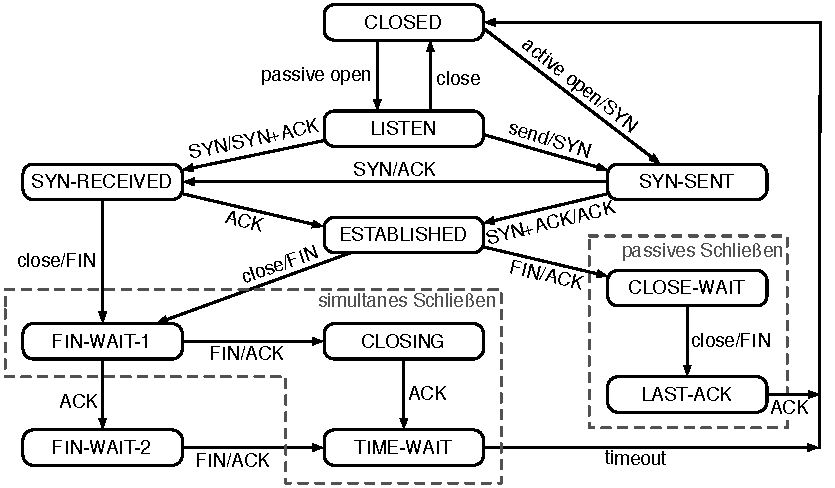
\includegraphics[bb=0bp 0bp 140mm 83mm,clip]{tcpudp/tcp_fsm}

\caption{\label{fig:tcp_fsm}Zustands�bergangsdiagramm}

\end{figure}


Das Diagramm verwendet die �bliche Notation f�r Zustands�bergangsdiagramme,
wobei alle in Gro�buchstaben verfassten Bezeichner entweder empfangene
Segmente (vor dem /) bzw. gesendete Segmente (nach dem /) angeben.
Die in Kleinbuchstaben angegebenen Bezeichner ,,close'', ,,passive
open'' und ,,active open'' geben Funktionen an, die der Anwendungsprozess
aufruft und der Bezeichner ,,timeout'' kennzeichnet einen Zeitablauf.

Drei Punkte gibt es zu beachten:
\begin{enumerate}
\item Auch wenn das ACK vom Client an den Server verloren geht, funktioniert
die Verbindung noch korrekt. Das liegt daran, dass der Client sich
schon im Zustand ESTABLISHED befindet und der Server zwar noch im
Zustand SYN\_RECEIVED ist, aber beim n�chsten empfangenen Segment
in den Zustand ESTABLISHED wechselt. Dieser Wechsel in ESTABLISHED
kann deshalb durchgef�hrt werden, da das Flag ACK in jedem Datensegment
gesetzt ist und das Feld Acknowledgment den korrekten Wert enth�lt.
Das ist wichtiger Punkt in TCP: Jedes Segment meldet, welche Sequenznummer
als n�chstes erwartet wird, auch wenn sich dabei die gleiche Sequenznummer
wiederholt, die in einem der vorherigen Segmente enthalten war.
\item Der �bergang von LISTEN nach SYN\_SENT ist im TCP Standard vorgesehen,
aber wird in der Regel von keiner TCP Implementierung dem Anwenerprozess
als Funktion zur Verf�gung gestellt: In den Zustand LISTEN kommt man
vom Zustand CLOSED mittels passiven �ffnen, das durch einen Funktionsaufruf
am Server erfolgt. Normalerweise kann danach nicht direkt gesendet
werden.
\item Viele Zustands�berg�nge sind nicht eingezeichnet. Kommt innerhalb
eines gesetzten Timeouts kein Acknowledgment an, dann wird das Segment
neu gesendet. Diese Neu�bertragungen sind nicht eingezeichnet. Nach
mehreren Versuchen gibt TCP auf und wechselt in den Zustand CLOSED.
\end{enumerate}

\subsubsection{Verbindungsabbau}

Beim Abbau einer Verbindung ist es wichtig, dass die Anwendungsprozesse
auf beiden Seiten die Verbindung schlie�en. Schlie�t nur eine Seite
die Verbindung bedeutet das, dass diese Seite keine Daten mehr senden
darf, aber sehr wohl noch bereit f�r den Empfang von Segmenten sein
muss. Aus diesem Grund ist das Zustands�bergangsdiagramm f�r den Abbau
einer Verbindung komplizierter, weil die M�glichkeit beachtet werden
muss, dass beide Seiten die close Funktion aufrufen. Ferner besteht
die M�glichkeit, dass zuerst die eine Seite und sp�ter die andere
Seite close aufruft. Daraus resultieren drei M�glichkeiten:
\begin{itemize}
\item Ein Anwenderprozess initiert den Verbindungsabbau mittels ,,close''.
\item Der entfernte Kommunikationspartner initiert den Verbindungsabbau
mittels Senden eines ,,FIN'' (passives Schlie�en).
\item Beide Anwenderprozesse wollen gleichzeitig die Verbindung mittels
,,close'' beenden (simultanes Schlie�en).
\end{itemize}
Da beide Partner die Verbindung abbauen m�ssen, kommt es zum Austausch
von insgesamt 4 Segmenten. Allerdings kann das ACK Segment und das
FIN Seqment, die der Host sendet, der passives Schlie�en durchf�hrt
in ein Segment zusammengefasst werden. Damit werden -- analog zum
Verbindungsaufbau -- ebenfalls nur 3 Segmente versendet.

Das Timeout vom Zustand TIME-WAIT ist notwendig, dass sicher ist,
dass das ACK angekommen ist bzw. dass es zu keiner �berschneidung
mit einer folgenden Verbindung kommt.


\subsection{Daten�bertragung}


\subsubsection{Segmentierung\label{sec:tcp_segmenting}}

Aus Sicht der Anwendung stellt TCP als Schnittstelle zwei Byte-Streams
zur Verf�gung. Ein Byte-Stream wird zum Lesen und einer zum Schreiben
verwendet. Das hei�t die Anwendung kann einzelne Bytes mittels dieser
Streams schreiben bzw. lesen. 

Andererseits werden in der Internet-Schicht IP Pakete �bertragen und
es w�re sehr ineffizient jedes Byte in einem eigenen IP Paket zu versenden.
Das Verh�ltnis von Header Daten zu Nutzdaten w�re sehr ung�nstig.
Aus diesem Grund speichert TCP die Bytes in einem Puffer zwischen
und erzeugt daraus eine Folge von Segmenten. Diese Segmente werden
mittels IP Paketen �bertragen und auf der Empf�ngerseite wieder in
TCP Segmente zur�ckgewandelt. Auf der Empfangsseite werden diese Segmente
wieder in einem Puffer gespeichert und der Anwendung als Byte-Stream
zur Verf�gung gestellt.

Daraus folgt, dass gro�e Segmente im Grunde die effizientere Wahl
darstellen. Es gibt allerdings zwei Gr�nde, die gegen eine gro� gew�hlte
Segmentgr��e sprechen: Einerseits kommt es dann zu langen Wartezeiten,
bis Seqmente versendet werden und andererseits kommt es wahrscheinlich
zur Fragmentierung, da die Segmente bei dem Transport �ber Netztechnologien,
die eine MTU aufweisen, die kleiner ist als das in ein IP Datagram
verpackte Segment.

Das Versenden eines Segmentes h�ngt von drei Kriterien ab:
\begin{itemize}
\item Die maximale Segmentgr��e (engl. maximum segment size, MSS) ist erreicht.
MSS definiert die Anzahl der Bytes, die als Nutzdaten in einem TCP
Segment gesendet werden k�nnen. Da die Header von IP und TCP zusammen
mind. 40 Bytes gro� sind, muss die MSS um mind. 40 Bytes kleiner sein
als die MTU. Im Falle von Ethernet betr�gt die MSS also 1460 Bytes.
Wird z.B. allerdings PPP �ber Ethernet verwendet, vermindert sich
um weitere 8 Byte auf 1452 Bytes.
\item Die Anwendung w�nscht einen sofortigen Versand (push).
\item Der Timer, der beim Einspeisen eines Bytes in den Sendepuffer gestartet
wird l�uft ab. D.h. es wurde eine gewissse Zeit von der Anwendung
keine neuen Daten in den Stream geschrieben.
\end{itemize}

\subsubsection{Sliding-Window\label{sec:tcp_sliding_window}}

Das Prinzip Sliding-Window Algorithmus wurde schon detailiert im Abschnitt
\vref{sec:sliding-window} beschrieben. Der in TCP implementierte
Algorithmus unterscheidet sich in folgenden Punkten von dem schon
beschriebenen Algorithmus:
\begin{enumerate}
\item Die Fenstergr��e in TCP hat keine feste Gr��e, sondern wird dem Sender
mittels des ,,Window'' Feldes im TCP Header bekanntgegeben. Das
bedeutet, dass der Empf�nger das ,,Window'' Feld im TCP Header auf
Grundlage der freien Puffergr��e ausw�hlt (siehe auch n�chsten Punkt).
\item In der TCP Variante wird auch noch der Sendepuffer und der Empfangspuffer
beachtet (siehe \vref{sec:tcp_segmenting}). 
\end{enumerate}
Mit jeder Best�tigung eines Segmentes sendet der Empf�nger auch die
neue Windowgr��e mit. Kann der Empf�nger keine weiteren Daten annehmen,
wird in der Best�tigungsantwort der Wert 0 f�r ,,Window'' gesetzt.
Damit wei� der Sender, dass der Empf�nger derzeit keine weiteren Daten
annehmen kann. Damit stellt sich allerdings die Frage, wie der Sender
wei� wann er wieder mit dem Senden fortfahren kann. Das Problem wird
folgenderma�en gel�st: Der Sender sendet in regelm��igen Abst�nden
Segmente mit der Datenl�nge 1 mit dem Wissen, dass diese Daten wahrscheinlich
verworfen werden. Kann der Empf�nger wieder Daten annehmen, dann wird
er dieses 1 Byte lange Datum annehmen und mit einer Best�tigungsnachricht
mit neu gesetzter ,,Window'' Gr��e reagieren.

In diesem Zusammenhang ist es wichtig darauf hinzuweisen, dass ein
ACK nicht bedeutet, dass der Anwenderprozess die Daten entgegengenommen
hat!


\subsubsection{Flusskontrolle\label{sec:tcp_flow_control}}

Wie schon beschrieben ist es die Aufgabe der Flusskontrolle den Empf�nger
vor �berlauf zu sch�tzen. Kommen mehr Segmente beim Empf�nger an als
dieser in seinem Puffer zwischenspeichern kann, dann werden diese
Segmente vom Empf�nger verworfen. In TCP wird die Flusskontrolle mittels
des Sliding-Window Algorithmus (siehe Abschnitt \vref{sec:tcp_sliding_window})
realisiert.

Das bedeutet, dass TCP ein Verfahren mit positiven Quittungen implementiert,
die Summenquittungen darstellen.


\subsubsection{�berlastkontrolle}

Unter �berlastkontrolle versteht man die Mechanismen zur Vermeidung
von �berlastung des Netzes (engl. congestion avoidance). Im Gegensatz
zur Flusskontrolle, dessen Aufgabe es ist, den Empf�nger vor �berlauf
zu sch�tzen, werden mittels Mechanismen der �berlastkontrolle die
Router am Weg zwischen Sender und Empf�nger gesch�tzt.

Eine �berlastsituation kann im Netz leicht entstehen, obwohl u.U.
keine �berlast in einem Empf�nger auftritt. Senden viele Sender �ber
einen Router, dann kann dieser leicht �berlastet werden. Diese Situation
verschlimmert sich noch weiter dadurch, dass in TCP verlorengegangene
Segmente eine erh�hte Netzaktivit�t hervorrufen, da es zu sinnlosen
Wiederholungen kommen kann, wenn die Best�tigungen den Sender erst
nach Ablauf des Timeouts erreichen.

Da die �berlastkontrolle in TCP jedoch beim Sender angesiedelt ist,
ben�tigt dieser Informationen �ber die Netzauslastung, um seine Sendegeschwindigkeit
an die aktuelle Situation anpassen zu k�nnen. Das ist jedoch das Schwierige
an der �berlastkontrolle, da der Sender diese Information nicht direkt
vom Netz erfragen kann, sondern diese indirekt ermitteln muss.

Folgende grundlegende Mechanismen zur �berlastkontrolle sind direkt
in TCP vorhanden, wobei es auch etliche fortgeschrittene Verfahren
gibt:


\minisec{Nagle-Algorithmus}

Betrachten wir nochmals den Aspekt wann ein Segment zu senden ist,
diesmal jedoch unter dem Gesichtspunkt der �berlastkontrolle: Gehen
wir davon aus, dass der Sender MSS Daten-Bytes senden will und das
Fenster um zumindest diese Anzahl an Bytes offen ist. In diesem Fall
wird der Sender senden, wenn einer der F�lle eintritt, die im Abschnitt
\vref{sec:tcp_segmenting} beschrieben sind. Was passiert jedoch,
wenn das Fenster nur zur H�lfte offen ist? Soll kein Segment gesendet
werden oder soll ein Segment mit der H�lfte der Bytes gesendet werden?

Der Standard definiert diesbez�glich kein Vorgehen. In den ersten
TCP Implementierungen wurde die Entscheidung getroffen, die H�lfte
der Datenbytes zu senden. Es stellte sich jedoch heraus, dass genau
dieses Vorgehen zu einer �berlastung des Netzes f�hren kann. Es trat
das sogenannte ,,Silly-Window-Syndrom'' auf: Gehen wir davon aus,
dass der Puffer des Empf�ngers voll ist und der Empf�nger deshalb
keine weiteren Daten annehmen kann. Gehen wir weiters davon aus, dass
die Anwendung am Empf�nger ein einziges Byte aus dem Puffer ausliest.
D.h. es kann eine Best�tigung zum Sender gesendet werden, die eine
Fenstergr��e von 1 enth�lt. Worauf der Sender wieder ein Segment mit
der Datenl�nge 1 senden kann. Wenn der Empf�nger wieder genau ein
Byte ausliest, dann wird wieder eine Best�tigung mit der Fenstergr��e
1 zur�ckgesendet. D.h. das Netz wird mit vielen kleinen Segmenten
�berschwemmt, wodurch eine potentielle �berlastsituation entsteht.

Das Silly-Window-Syndrom stellt nur dann ein Problem dar, wenn entweder
der Sender ein kleines Segment �bertr�gt oder der Empf�nger das Fenster
nur ein wenig �ffnet.

Wie kann man mit dieser Situation umgehen? Man kann einfach eine gewisse
Zeit warten bis verf�gbare Daten gesendet werden. Die Frage ist wie
lange eine vern�nftige Zeitdauer bemessen ist. Wird zu lange gewartet,
dann werden interaktive Anwendungen wie telnet oder ssh beeintr�chtigt.
Wird hingegen zu kurz gewartet, dann entsteht wieder das Silly-Window-Syndrom.

TCP implementiert den sogenannten Nagle-Algorithmus, der nach John
Nagle benannt ist. Die zugrundeliegende Idee ist, dass der Sender
irgendwann ein ACK empfangen wird, solgange TCP Daten unterwegs sind.
Dieses ACK kann wie ein Timerablauf behandelt werden, wobei dadurch
die �bertragung von mehr Daten angesto�en wird.

Wenn die Anwendung sendebereite Daten produziert, dann:
\begin{enumerate}
\item Wenn sowohl die verf�gbaren Daten als auch das Fenster $\geq$ MSS,
dann sende Daten.
\item Anderenfalls: Wenn unbest�tigte Daten anstehen, 

\begin{enumerate}
\item dann puffere die neuen Daten bis ein ACK kommt.
\item Anderenfalls: Sende alle neuen Daten jetzt.
\end{enumerate}
\end{enumerate}
Um interaktive Anwendungen vom Nagle-Algorithmus nicht zu beeintr�chtigen,
besteht die M�glichkeit diesen auszuschalten. Dies geschieht �ber
das Socket-API mittels der Option TCP\_NODELAY.


\minisec{Slow-Start}

Am Anfang einer �bertragung ist noch keine Information �ber die Auslastung
eines Netzes bekannt. Die Idee ist, die Senderate langsam zu steigern
bis entweder der Fall eines Segmentverlustes oder ein ACK-Timeout
eintritt.


\minisec{Fast-Retransmit}

Die Idee von Fast-Retransmit ist, nach einem Paketverlust schneller
auf eine Stausituation zu reagieren. Dazu informiert der Empf�nger
den Sender, wenn Pakete au�er der Reihe ankommen und somit ein Paketverlust
vorliegt. Das wird dadurch erreicht, dass der Empf�nger das zuletzt
korrekt empfangene Paket f�r jedes au�er der Reihe empfangene Paket
jedes Mal neu best�tigt. Diese mehrfach versendeten Best�tigungen
werden ,,Dup-Acks'' genannt. Hat der Sender drei solcher Dup-Acks
erhalten schlie�t er daraus, dass ein Paket verloren gegangen ist
und sendet es auch vor Ablauf des Timeout wieder an den Empf�nger.
Au�erdem schlie�t der Sender, dass Folgepakete sehr wohl angekommen
sind und erh�ht das Sendefenster um die Anzahl der empfangenen Dup-Acks.



\chapter{Protokolle der Anwendungsschicht}

Hier werden die wichtigsten Protokolle besprochen, die der Anwendungsschicht
zuzurechnen sind und trotzdem f�r den Betrieb eines TCP/IP Netzes
notwendig sind.


\section{DHCP\label{sec:DHCP}}

siehe Foliensatz!

%% Um einem Host automatisch mit einer IP Adresse, einer Subnetzmaske,
%% einen Default-Router, einen DNS-Server oder Proxy-Konfigurationen
%% zu versorgen, kann DHCP (dynamic host configuration protocol, RFC
%% 2131) herangezogen werden.

%% Die prinzipielle Funktionsweise ist folgende:
%% \begin{itemize}
%% \item Es existiert zumindest ein DHCP Server, der die Parameter f�r das
%% Netz gespeichert hat.
%% \item Wird ein f�r DHCP konfigurierter Host hochgefahren, dann sendet er
%% eine DHCPDISCOVER Nachricht mittels UDP an die IP Broadcast-Adresse
%% (also 255.255.255.255) mit dem Zielport 67 und einem Absender 0.0.0.0
%% vom Quellport 68. Diese Nachricht enth�lt nat�rlich au�erdem die MAC
%% Adresse des zu konfigurierenden Hosts.
%% \item Ein in diesem Netz vorhandener DHCP Server wird diese Nachricht empfangen
%% mit einer DHCPOFFER Broadcast-Nachricht vom UDP Quellport 68 zur Adresse
%% 255.255.255.255 mit dem UDP Zielport 67 antworten. Diese Nachricht
%% enth�lt einen Vorschlag f�r eine IP Adresse, u.U. weitere Parameter
%% als auch eine Lease und einen Serveridentifier. Eine Lease bedeutet
%% die Angabe einer Zeit, wie lange der Host diese IP Adressen samt den
%% �bermittelten Parametern verwenden darf. Der Host muss sich rechtzeitig
%% vor Ablauf dieser Lease um eine Verl�ngerung beim DHCP Server bem�hen.\\
%% Der Vorschlag kann entweder auf Grund der MAC Adresse statisch
%% konfiguriert sein oder aus einem Pool von IP Adressen vom DHCP Server
%% dynamisch vergeben werden.
%% \item Da es mehrere DHCP Server in einem Netz geben darf, kann der Host
%% jetzt unter den Angeboten w�hlen (z.B. den Server, der die l�ngste
%% Lease anbietet). Er sendet eine Broadcast-Nachricht DHCPREQUEST mit
%% dem Serveridentifier. Alle anderen DHCP Server werden dies als Absage
%% werten und nicht weiter reagieren. Der vom Host ausgew�hlte DHCP Server
%% wird mit einer DHCPACK Nachricht die Zuordnung best�tigen oder mit
%% einer DHCPNAK Nachricht die Zuordnung verweigern.
%% \item Der Client wird sich standardm��ig nach der H�lfte der Lease erneut
%% mittels DHCPREQUEST (allerdings per Unicast) beim Server um eine Verl�ngerung
%% ansuchen. Der Server wird in der Regel mit den identischen Daten best�tigen.
%% Antwortet der Server jedoch nicht, kann der Client die Adresse weiterverwenden,
%% muss allerdings nach 7/8 der Zeit erneut um eine Verl�ngerung ansuchen
%% (per Broadcast).
%% \end{itemize}
%% Folgende Punkte sind interessant:
%% \begin{itemize}
%% \item Die Verwendung mehrerer DHCP Server kann durchaus sinnvoll sein, um
%% eine Redundanz und damit eine Ausfallsicherheit zu erreichen.
%% \item Es macht keinen Sinn in jedem Teilnetz einen DHCP Server zu betreiben.
%% Um trotzdem DHCP betreiben zu k�nnen, ist es lediglich notwendig in
%% jedem Teilnetz einen DHCP-Relay-Agenten zu konfigurieren. Dieser reagiert
%% auf alle DHCP Nachrichten und leitet sie per Unicast an den eigentlichen
%% DHCP Server weiter.
%% \item Es gibt DHCP Server, die mit einem DNS Server zusammenarbeiten und
%% diesen �ber die Vergabe einer Zuordnung von IP Adresse, Rechnernamen
%% und Lease informieren. Dies wird als dynamisches DNS, abgek�rzt DDNS
%% (engl. dynamical DNS), bezeichnet.
%% \end{itemize}

\section{DNS\label{sec:DNS}}

siehe Foliensatz!

%% Das Domain Name System (DNS) ist ein verteiltes, hierarchisches System
%% zur Aufl�sung von Namen in IP-Adressen und umgekehrt. Dieses System
%% erm�glicht damit eine Positionstransparenz als auch eine Migrationstransparenz.
%% Der gro�e Vorteil liegt in der Flexibilit�t und der Wartbarkeit der
%% Zuordnungen.

%% Es existiert keine zentrale Datenbank. Der Namensraum ist baumartig
%% in Zonen aufgeteilt f�r die jeweils unabh�ngige Administratoren zust�ndig
%% sind. Diese Zonen werden von DNS Servern verwaltet. Die Wurzel dieses
%% Baumes wird mit einem ,,.'' bezeichnet.


%% \subsection{Teile des DNS}

%% Das DNS besteht aus drei Komponenten:
%% \begin{itemize}
%% \item Der Domainname (fully qualified domain name, FQDN) besteht aus einer
%% Folge von sogenannten ,,Labels'', die aus Zeichenketten (alphanummerisch
%% und der Bindestrich), die durch Punkte von einander getrennt sind.
%% Beispiel: ,,htlwrn.ac.at\underbar{.}''. Ein Domainname wird mit
%% einem Punkt abgeschlossen, der normalerweise jedoch weggelassen wird.
%% So ein Domainname ist case-insensitive und darf inklusive aller Punkte
%% maximal 255 Zeichen lang sein. Jedes Label darf maximal 63 Zeichen
%% lang sein.


%% Die direkt unter der Wurzel befindlichen Dom�nen werden als Top Level
%% Domains (TLD) bezeichnet. An TLD gibt es entweder L�nderk�rzel (als
%% ISO 3666) wie ,,.at'' oder generische TLD wie ,,.com'', ,,.org'',
%% ,,.net'', ,,.name'' oder ,,.info''. Die TLD ,,.eu'' liegt
%% in gewisser Hinsicht in der Mitte.

%% Um auch nicht ASCII Zeichen in Domain-Namen verwenden zu k�nnen, wurde
%% das Konzept IDN (Internationalized Domain Name) eingef�hrt, das ein
%% Verfahren angibt wie Dom�nennamen mit Unicode Zeichen in ASCII Zeichen
%% umgesetzt werden. Diese Umsetzung wird direkt vom Client durchgef�hrt,
%% sodass das neue System kompatibel zur bestehenden Infrastruktur ist.

%% \item Die Nameserver (DNS Server) sind diejenigen Programme, die Anfragen
%% zum Domain-Namen beantworten. Es wird zwischen autoritativen (diese
%% sind f�r eine Zone verantwortlich) und nicht autoritativen Nameservern
%% (sind nicht f�r eine Zone verantwortlich) unterschieden. Nicht autoritative
%% Nameserver beziehen ihre Informationen �ber eine Zone von autoritativen
%% oder auch nicht autoritativen Nameservern und halten schon beantwortete
%% Anfragen in einem Cache.
%% \item Ein Resolver (DNS Client) ist direkt in TCP integriert und steht dem
%% Anwenderprozess als Funktion zur Verf�gung.
%% \end{itemize}

%% \subsection{Zonen}

%% Da es sich beim DNS vom Prinzip her um eine verteilte Datenbank mit
%% einem hierarchischen Aufbau der Eintr�ge handelt, wird die Verwaltung
%% der Eintr�ge in Zonen aufgeteilt. Eine Zone ist ein zusammenh�ngender
%% Teil des Dom�nen-Baumes, f�r den diese Zone autoritative Informationen
%% zur Verf�gung stellt.

%% Das bedeutet, dass eine Zone f�r einen gewissen Teil dieses Baumes
%% verantwortlich ist. Damit ist eine Zone f�r die Domain und eventuell
%% f�r die Subdomains verantwortlich, wenn die Subdomains nicht wiederum
%% in eine Zone ausgelagert sind.

%% F�r jede Zone muss es mindestens 2 DNS Server geben, die f�r diese
%% Zone Anfragen entgegeben nehmen. Dies wurde aus Gr�nden der Ausfallsicherheit
%% so festgelegt.


%% \subsection{Namensaufl�sung}

%% Im Zuge der Namensaufl�sung wird zwischen rekursiver und iterativer
%% Namensaufl�sung unterschieden:
%% \begin{itemize}
%% \item Die rekursive Namensaufl�sung funktioniert so, dass der Resolver den
%% konfigurierten Nameserver kontaktiert. Kennt dieser die Antwort nicht,
%% dann fragt dieser selbstst�ndig bei weiteren Nameservern nach und
%% liefert danach die Anwort an den Client zur�ck.
%% \item Bei der iterativen Namensaufl�sung liefert der Nameserver lediglich
%% die Adresse des n�chsten abzufragenden Nameserver zur�ck, falls er
%% die Antwort nicht kennt und der Resolver muss selber die weiteren
%% Anfragen durchf�hren.
%% \end{itemize}
%% Die Unterscheidung welche der beiden Varianten bei einer Anfrage verwendet
%% wird, h�ngt von einem Flag in der Anfrage ab. Ein Resolver wird in
%% der Regel eine rekursive Namensaufl�sung verlangen. Ein Root-Server
%% akzeptiert nur iterative Anfragen.

%% Unter einer inversen Anfrage versteht man die Aufl�sung der IP Adresse
%% in einen Dom�nennamen. Dazu gibt es eine eigene vordefinierte Dom�ne
%% namens in-addr.arpa, die folgenderma�en verwendet wird: Angenommen
%% es soll f�r die IP Adresse 193.170.149.127 der Dom�nenname gefunden
%% werden, dann wird folgender Dom�nenname 127.149.170.193.in-addr.arpa
%% beim DNS Server zur Aufl�sung www.htlwrn.ac.at f�hren.


%% \subsection{Typen von DNS-Servern}


%% \minisec{Master- und Slave-Server}

%% Wie schon besprochen muss es f�r jede Zone mindestens 2 autoritative
%% DNS Server geben. Genauer es muss genau einen prim�ren Master-Server
%% und einen oder mehrere Slave-Server geben. �nderungen werden nur am
%% prim�ren Master-Server vorgenommen. Die Slave-Server fordern eine
%% Kopie der Zonen-Datei an und laden sie von diesem herunter.

%% Master und Slave sind lediglich Rollen. Ein Slave-Server kann durchaus
%% auch Master-Server sein, wenn ein anderer Slave-Server die Zonen-Datei
%% anfordert. Es kann jedoch nur einen prim�ren Master-Server geben.
%% Alle anderen sind sekund�re Server f�r eine Zone.

%% �nderungen an der Zonen-Datei werden von einem Slave-Server dadurch
%% erkannt, dass jede �nderung der Zonen-Datei eine Inkrementierung der
%% Seriennummer der Zonendatei um 1 bewirkt.


%% \minisec{Caching-Server}

%% Master-Server und Slave-Server geben autoritative Antworten. Von einem
%% Caching-Server erh�lt man keine autoritative Antworten. Dies liegt
%% darin begr�ndet, dass ein Caching-Server keine Kopie der Zonen-Datei
%% enth�lt. Er speichert lediglich schon einmal ermittelte Antworten
%% in einem Cache. Die Eintr�ge werden f�r eine gewisse Zeit in diesem
%% Cache zwischengespeichert. Solange eine Antwort im Cache liegt, kann
%% der Caching-Server diese Antwort im Zuge einer Anfrage zur�ckliefern
%% und muss keine eigene Anfrage stellen.


%% \minisec{Forwarder}

%% Ein Forwarder leitet eine Anfrage immer weiter und zwar immer an den
%% selben DNS-Server. Damit dient er lediglich als Zwischenstation.


\section{Routingprotokolle\label{sec:routing_protocols}}

In Abh�ngigkeit, ob ein Router ein Teil eines autonomen Systems (ein
oder mehrere Netze, die von einer Organisation verwaltet werden) ist
oder an der Grenze eines autonomen Systems eingesetzt wird, verwendet
man verschiedene Arten von Routingprotokollen:
\begin{labeling}{00.00.0000}
\item [{Interior~Gateway~Protocol~(IGP)}] Es handelt sich um einen Typ
von Routing-Protokollen, die ausschlie�lich innerhalb eine autonomen
Systems zum Einsatz kommt. Beispiele sind: RIP und OSPF. RIP (routing
information protocol) ist das am h�ufigsten eingesetzte Protokoll
und verwendet den Distanzvektor-Algorithmus (siehe Abschnitt \vref{sec:distance-vector-algorithm}),
w�hrend OSPF (open shortest path first) den Link-State-Algorithmus
(siehe Abschnitt \vref{sec:link-state-algorithm}) verwendet.


RIP wird nur in kleineren Organisationen eingesetzt. Dies liegt einerseits
an den schon im Abschnitt \ref{sec:distance-vector-algorithm} erl�uterten
Nachteilen des eingesetzten Verfahrens, aber auch daran, dass z.B.
immer nur die Hops als Gewichte herangezogen werden. Damit w�rde eine
ISDN Verbindung, die �ber einen Hop geht einer hoch performanten Standleitung
mit 2 Hops der Vorzug gegeben werden. Au�erdem kann die Anzahl der
Hops 15 ja nicht �berschreiten.

OSPF f�hrt eine Wertigkeit der Links ein und kann damit einer Standleitung
den Vorzug gegen�ber einer ISDN Leitung geben. Allgemein findet es
eine optimale Route auf Grund mehrerer Kriterien und unterteilt au�erdem
noch in sogenannte Areas, um effiziente eine Router-Tabellen-�bertragung
zu erreichen. OSPF ist ein bedeutend komplexeres Protokoll.

\item [{Exterior~Gateway~Protocol~(EGP)}] Diese werden zwischen Routern
autonomer Systeme eingesetzt. Beispiele sind: BGP, EGP (nicht mehr
in Verwendung).
\end{labeling}




\chapter{NAT\label{sec:NAT}}

NAT (Network Address Translation) ist in Rechnernetzen der Sammelbegriff
f�r Verfahren, um automatisiert und transparent Adressen in IP Paketen
durch andere Adressen zu ersetzen. Diese Adressumsetzung wird in der
Regel zwischen einem �ffentlichen und einem internen Netz durchgef�hrt.

Der Haupteinsatz von NAT besteht darin Netze mit privaten IP Adressen
an das �ffentliche Internet anzubinden und damit auch �ffentliche
IP Adressen zu sparen. In gewisser Weise kann es auch als eine Sicherheitsma�nahme
eingesetzt werden, auch wenn dies nicht die prim�re treibende Absicht
ist.

Das Prinzip ist, dass am Router, der das interne vom �ffentlichen
Netz trennt eine Umsetzungstabelle enthalten ist, die eine Abbildung
der privaten IP Adressen auf die �ffentlichen IP Adressen enth�lt.
Unter Umst�nden enth�lt diese Umsetzungstabelle weitere Informationen,
um die Abbildung eindeutig zu machen.

Um komplexere Protokolle (wie ftp oder VoIP) �ber einen NAT-Router
betreiben zu k�nnen, muss der NAT-Router allerdings als ein Gateway
fungieren.

NAT hat trotz des komplexeren Systemaufbaus sicher dazu beigetragen,
dass die Anzahl der freien IPv4 Adressen viel langsamer abgenommen
hat.

Es gibt zwei grundlegende Formen von NAT, die in den beiden folgenden
Abschnitten kurz besprochen werden.


\section{Source-NAT}

Beim Source-NAT (SNAT) wird bei einer Anfrage eines Clients im lokalen
Netz an einen Server im Internet die private Client-Adresse auf eine
verf�gbare externe Adresse ge�ndert. Es gibt prinzipiell drei M�glichkeiten:
\begin{labeling}{00.00.0000}
\item [{Statisches~SNAT}] Hierbei wird jeder privaten Adresse genau eine
externe Adresse zugeordnet. D.h. es gibt eine 1:1 Abbildung von lokalen
zu extern verf�gbaren Adressen. Dies kann notwendig sein, wenn der
interne Rechner als Server im Internet verf�gbar sein soll oder wenn
man die Sicherheit erh�hen will (Struktur des internen Netzes wird
nicht preisgegeben).
\item [{Dynamisches~SNAT}] Sind mehr lokale Rechner vorhanden als externe
Adressen zur Verf�gung stehen, muss die Zuordnung von lokaler zu externer
Adresse dynamisch vorgenommen werden. Die Zuordnungstabelle im NAT-Router
kann noch mit zus�tzlichen Informationen wie z.B. Portangaben versehen
werden, sodass auch gleichzeitig mehr interne Rechner mit Servern
im Internet kommunizieren k�nnen als externe Adressen zur Verf�gung
stehen.
\item [{Masquerading}] Es handelt sich um eine Sonderform bei der alle
internen Adressen auf \emph{eine} externe Adresse abgebildet werden.
\end{labeling}

\section{Destination-NAT}

Das Destination-NAT (DNAT) ist im Grunde die Umkehrung des SNAT: Es
wird die Ziel-Adresse abgebildet. Ein externer Client sendet eine
Anfrage an eine extern verf�gbare Adresse unseres Netzes (z.B. an
die Adresse des NAT-Routers). Der NAT-Router bildet die Zieladresse
z.B. auf die interne Adresse des DMZ Servers ab und leitet daher diese
Anfrage an den DMZ Server weiter. Hier gibt es prinzipiell zwei M�glichkeiten:
\begin{itemize}
\item Der NAT-Router leitet alle Anfragen bzgl. einer extern verf�gbaren
Adresse an den DMZ Server weiter.
\item Der NAT-Router leitet Anfragen bzgl. einer extern verf�gbaren Adresse
an die externe Adresse weiter, wenn zus�tzliche Kriterien zutreffen.
Das wichtigste Kriterium ist die Portangabe. D.h. nur wenn die Portangabe
z.B. 80 ist wird an den internen DMZ Server weitergeleitet.
\end{itemize}




\chapter{IPv6}

Die wesentlichen funktionellen Unterschiede zu IPv4 sind:
\begin{itemize}
\item Adressraum: Einer der Beweggr�nde IPv6 zu entwickeln, war die geringe
Anzahl an freien Adressbereichen. IPv6 hat 128 Bit lange Adressen.
D.h. es gibt ca. $3.4\cdot10^{38}$ m�gliche Adressen. Die Notation
wird nicht mehr byteweise in Dezimalschreibweise durch Punkte getrennt,
sondern wortweise (16 Bit) in Hexadezimalschreibweise durch Doppelpunkte
getrennt angegeben. Z.B.: 2002:89d0:e02e::89d0:e02e.
\item Durch die hohe Anzahl an verschiedenen Adressen besteht die M�glichkeit
diese geographisch-hierarchisch zu vergeben. Dadurch k�nnen die Anzahl
der Routereintr�ge weiter gesendet werden.
\item Es wurde eine lokale Adressvergabe eingef�hrt, sodass Adressen automatisch
vergeben werden. Dazu kann sich ein Host eine IPv6 Adresse direkt
aus einer MAC Adresse geben und mit angrenzenden Hosts und Routern
diesbez�glich abstimmen.
\item Es gibt im IP Header keine Checksumme mehr. D.h. alle �berpr�fungen
m�ssen durch h�here Protokolle erledigt werden. Das liegt daran, dass
viele Router die Checksum �berhaupt nicht �berpr�ft haben, sondern
einfach um eins erh�ht (wg. dem Header TTL) haben.


Der Basisheader wurde generell k�rzer gestaltet. Er enth�lt nur mehr
7 anstatt 13 Felder. Es kann allerdings auch mehrere Header geben.
Diese �nderungen erm�glichen Routern Paket schneller zu verarbeiten.

\item Sicherheitsfunktionen wurden direkt eingebaut und basieren auf IPSec.
IPSec kann zwar auch mit IPv4 verwendet werden, ist aber in IPv6 direkt
integriert.
\item Die Fragmentierung der Datenpakete in Routern wurde entfernt. M�sste
ein Paket fragmentiert werden, dann wird eine Fehlermeldung an den
Sender zur�ckgeschickt, der daraufhin die MSS anpassen muss und erneut
sendet.
\item QoS wurde ebenfalls integriert. Ziel ist die verbesserte �bertragung
von Audio und Videodaten sowie die �bertragung von Daten in Echtzeit.
\item Weiters gibt es zus�tzlich zu Broadcast und Multicast auch Anycast-Adressen.
\end{itemize}



\setpartpreamble[uc][14cm]{\vspace{3cm}Der Teil beschreibt wichtige
Dienste und Anwendungen f�r das Internet.}


\part{Dienste und Anwendungen\label{par:services_apps}}


\chapter{Entfernter Zugriff}


\section{FTP}

Datenzugriff mittels ftp (RFC 959) ist ein relativ altes und noch
immer sehr weit verbreitetes Protokoll. 

Anders als http ben�tzt ftp \emph{mehr} als eine Verbindung zwischen
Client und Server: Zun�chst baut der Client eine Verbindung zum Port
21 (Control Port) des Servers auf. Diese Verbindung dient zur Authentifizierung
und Befehls�bertragung. Zur eigentlichen Daten�bertragung wird bei
Bedarf eine eigene Verbindung aufgebaut.

Dazu gibt es \emph{2 Betriebsarten}:
\begin{description}
\item [{Active~Mode}] Der Server baut von seinem Port 20 (Data Port) eine
Verbindung zu einem vom Client gew�hlten Port (�ber 1023) auf. 
\item [{Passive~Mode}] Der Client baut eine Verbindung zu einem vom Server
gew�hlten Port auf (meistens beide gr��er 1023). 
\end{description}
Dieses Protokoll wird als relativ unsicher angesehen, da sowohl die
Passwort�bertragung als auch die Daten�bertragung unverschl�sselt
stattfindet. Technisch gesehen ist der Befehlskanal wie beim telnet
Protokoll aufgebaut. Aus diesem Grund sollte man Daten nur mit scp
(secure copy protocol) oder der Weiterentwicklung sftp (siehe \vref{sec:SSH})
arbeiten.


\section{Netzwerkdateisysteme}

Als Alternative zu einer �bertragung mit ftp, scp oder sftp kann f�r
den Datenzugriff ein Netzwerkdateisystem wie NFS (Network File System)
oder CIFS (Common Internet File System) verwendet werden.


\minisec{NFS}

NFS wurde von SUN entwickelt und stellt ein Netzwerkdateisystem f�r
Unix dar. NFS hat heutzutage keine dominante Bedeutung mehr. Viele
wichtige Punkte wie die Authentifizierung der Benutzer (und nicht
nur der Rechner wie in NFSv3) oder der Wegfall der Unix-Lastigkeit
wurden erst in NFSv4 eingef�hrt. Diese Version hat sich jedoch nicht
durchsetzen k�nnen.


\minisec{CIFS}

CIFS wurde 1996 von Microsoft bei der IETF eingereicht und stellt
eine Erweiterung von SMB (Server Message Blocks) dar. SMB wurde von
IBM mit dem Ziel entwickelt f�r DOS ein Netzwerkdateisystem zur Verf�gung
zu haben. Microsoft hat SMB weiterentwickelt und in ihre Produktlinie
integriert. CIFS bietet entfernten Zugriff auf Dateien, Drucker oder
andere Ger�ten als auch die M�glichkeit zur IPC.


\section{Entfernte Ausf�hrung}


\subsection{SSH\label{sec:SSH}}

siehe Foliensatz!

%% SSH ist nicht nur ein Protokoll (siehe Abschnitt \vref{sec:SSH_protocol}),
%% sondern auch eine Anwendung, die es erlaubt �ber das Netz sich auf
%% einem Rechner anzumelden und Befehle abzusetzen.

%% Es ersetzt unsichere Protokolle wie rsh, rlogin oder telnet. rcp kann
%% durch scp (secure copy) ersetzt werden und ftp durch sftp (secure
%% file transfer protocol). scp und sftp ersetzen die unverschl�sselten
%% Protokolle, haben ansonst aber keine Gemeinsamkeiten. Z.B. gibt es
%% bei sftp auch keinen getrennten Daten- und Befehlskanal. Es wird wie
%% f�r ssh der Port 22 verwendet.


\subsection{X-Window-Protokoll}

Mit dem X-Window-Protokoll kann man graphische Ausgaben zum Client
(dieser wird als Server bezeichnet) und Eingaben zum Server (das ist
der eigentliche Client) schicken.

�hnlich: Windows Terminal Server





\chapter{E-Mail}

siehe Foliensatz \emph{E-Mail}


%
\chapter{Internet}

Dieses Kapitel behandelt einige wichtige Standards und Protokolle,
die im Internet eine wichtige Rolle spielen.


\minisec{URI}

Unter einer URI (Uniform Resource Identifier, RFC 3986) versteht man
den �berbegriff zu einer URL (Uniform Resource Locator) und URN (Uniform
Resource Name). Eine URL stellt die Adresse einer Internetressource
dar. Die URL hat lediglich, dass Problem, dass eine `h�ngende Referenz'
entsteht, wenn die Ressource verschoben wird, d.h.~zu einem anderen
Host verlagert wird. Eine URN ist andererseits der dauerhafte Name
einer Internetressource.
\begin{description}
\item [{URL}] steht f�r Uniform Ressource Locator und wird im Web verwendet,
um Einheiten zu addressieren.


Der typische Aufbau einer URL ist folgenderma�en:
\begin{lyxcode}
protocol://hostname:port/pathname{[}?query{]}{[}\#anchor{]}
\end{lyxcode}
Beispiele:
\begin{lyxcode}
http://www.htlwrn.ac.at:80/index.html

http://www2.htlwrn.ac.at/ko/person.html\#top

http://www.google.at/index?q=php
\end{lyxcode}
Jeder Teil eines Dom�nennamens ist eine Zeichenkette (alphanumerisch,
als einziges Sonderzeichen ist `-' erlaubt) die mindestens ein Zeichen
und maximal 63 Zeichen lang sind. Ein Dom�nenname darf inklusive aller
Punkte maximal 255 Zeichen lang sein.

Derzeit d�rfen in URLs nur ASCII kodierte Zeichen vorkommen! Werden
andere Zeichen oder Zeichen, die im Pfad einer URL eine Bedeutung
haben (wie z.B. der Schr�gstrich), ben�tigt, dann sind diese zu maskieren:
\texttt{suche.cgi?name=G\%FCnter+Kolousek}
\begin{enumerate}
\item Die alphanummerischen Zeichen ,,a'' - ,,z'', ,,A'' - ,,Z''
und ,,0'' - ,,9'' bleiben gleich. 
\item Die Zeichen ,,.'', ,,-'', ,,{*}'' und ,,\_'' bleiben gleich
. 
\item Das Space Zeichen ,,~'' wird in ein ,,+'' gewandelt. 
\item Alle anderen Zeichen werden in ein oder mehrere Bytes gewandelt (W3C
empfiehlt UTF-8). Danach wird jedes Byte in einen 3-Zeichen String
gewandelt, ,,\%xy'', wobei xy eine hexadezimale Zahl mit 2 Ziffern
ist.
\end{enumerate}
Dies entspricht dem MIME Typ ,,application/x-www-form-urlencoded''.
Dieser Sachverhalt ist in der Benennung von Datei\-namen zu beachten!

Seit M�rz 2004 k�nnen deutsche, �sterreichische, schweizer und lichtensteiner
Dom�nen mit Umlauten registriert und verwendet werden. Um das neue
System mit dem bisherigen kompatibel zu halten, werden die erweiterten
Zeichens�tze mit erlaubten Zeichen kodiert, also auf derzeit g�ltige
Namen abgebildet (Punycode). 

\item [{URN}] Uniform Resource Name ist ein eindeutiger Name, der unabh�ngig
von der Adresse eine Ressource eindeutig identifiziert. Mit der URN
kann man bei einem ,,URN-Verzeichnsdienst'' die zugeh�rige URL erhalten.
Allerdings hat sich kein Verzeichnis f�r URN etablieren k�nnen. Eine
URN hat folgende Gestalt: \texttt{urn:Namensraum:Name}, z.B. urn:isbn:3-8266-1378-3.
\end{description}

\section{HTTP}

HTTP (hyper text transfer protocol) ist ein Client/Server Protokoll,
das urspr�nglich zur Abfrage von statischen Informationen entworfen
wurde.


\subsection{Beschreibung}
\begin{itemize}
\item Ist ein relativ einfaches, lightweight, zustandsloses Protocol. D.h.
der Server merkt sich keinen Zustand zwischen mehreren Anfragen eines
Clients.
\item Ist ein verbindungsloses Protokoll. D.h. jede Verbindung wird prinzipiell
nach jeder Abfrage wieder abgebaut (bis http/1.0).
\item Wurde urspr�nglich f�r die Abfrage rein statischer Information entworfen.
\item Ist ein zeichen-orientiertes Protokoll (im Gegensatz zu einem bin�ren
Protokoll)
\item Ist ein reines Request/Response Protokoll 

\begin{itemize}
\item Immer Client (user agent) beginnt request
\item kein callback des Servers zum Client
\item Client muss immer Verbindung aufbauen, Server schlie�t Verbindung
nach response (beide k�nnen vorzeitig die Verbindung abbrechen)
\end{itemize}
\item Verhandlung �ber Datenrepr�sentation 
\item funktioniert mit TCP. Der Standardport ist 80. 
\item Die erste Version von http war die Version 0.9, bei dem es sich um
eine einfache Version handelte. Version 1.0 ist eine verbesserte Version,
die haupts�chlich Nachrichten im MIME Format und Metainformation �ber
die Daten beinhaltet. Derzeit gibt es haupts�chlich Implementierungen
der Version 1.0 (RFC 1945) und der Version 1.1 (RFC 2616, 2817) von
http.


Ein wesentlicher Unterschied zwischen 1.0 und 1.1 liegt daran, dass
in http/1.0 der Server nach dem Senden der Antwort die Verbindung
zum Client geschlossen hat, wenn nicht der Header 'Connection: KeepAlive'
vom Client gesendet worden ist. In http/1.1 wird die Verbindung aufrechterhalten,
wenn nicht der Client explizit 'Connection: Close' gesendet hat. Aufgrund
der vielen Inline-Images, Applets und Frames wird dadurch viel Overhead
vermieden.

Andere Unterschiede betreffen die Unterst�tzung zum Cachen von Internet
Ressourcen und das Unterst�tzen mehrere Dom�nen zu einer IP Adresse.
Au�erdem ist das sogenannte `chunked encoding' hinzugekommen, das
es erlaubt bereits die Antwort zu senden ohne die L�nge der Antwort
zu kennen. 

\end{itemize}

\subsection{Http Request}
\begin{itemize}
\item zeilenorientierter Aufbau


\begin{tabular}{|l|l|}
\hline 
Methode Request-URI Protokoll\textbackslash{}r\textbackslash{}n & erste Zeile\tabularnewline
\hline 
(Key: Value\textbackslash{}r\textbackslash{}n){*} & beliebige Anzahl an Header Zeilen\tabularnewline
\hline 
\textbackslash{}r\textbackslash{}n & eine Leerzeile\tabularnewline
\hline 
(Daten)? & optionaler Datenblock\tabularnewline
\hline
\end{tabular}

\textbackslash{}r entspricht einem Carrige Return (ASCII 13) und \textbackslash{}n
entspricht einem Line Feed (ASCII 10).

Daten in einer URL werden (im speziellen bei einem GET Request, aber
auch bei einem POST Request) ,,urlencoded''. Meistens wird die Request-URI
als eine relative URL angegeben. D.h. es sieht die URL z.B. so aus:
/lva/prr.html. Es gibt jedoch folgendes dabei zu beachten: 
\begin{itemize}
\item Wird ein Proxy verwendet, dann sendet der Browser eine absolute URL
an diesen, damit dieser wei� an welchen Server er die Anforderung
weiter senden soll. Z.B. http://edvowww.htlwrn.ac.at/ko/prr5.html! 
\item http 1.1 konforme Server m�ssen absolute URLs verstehen! 
\end{itemize}
\item Verf�gbare Methoden (immer in Gro�buchstaben) 

\begin{description}
\item [{GET}] Die GET Anforderung wird ben�tigt, um ein Dokument herunterzuladen
(kein Datenbereich der Anforderung).


Bei der Request-URI kann es sich um einen Pfadnamen zu einem Dokument
aber auch die Angabe eines CGI Programmes handeln.

Wird ein Formular ausgef�llt und mit der GET Methode ausgef�hrt, dann
werden die ausgef�llten Felder an die Request-URI angeh�ngt.

Bsp.: \texttt{GET /cgi/greeetings.pl?name=max\&email=max@htlwrn.ac.at
HTTP/1.0} Beinhaltet der GET-Request einen If-Modified-Since Header,
dann werden die Daten nur im Bedarfsfall �bertragen. Auch damit kann
die Netzwerksbelastung gesenkt werden.

Die Semantik einer GET Anforderung ist, dass prinzipiell am Server
keine Ver�nderungen hervorgerufen werden sollen. D.h. mehrmaliges
Senden einer GET Anforderung soll prinzipiell immer zum selben Ergebnis
f�hren.

\item [{HEAD}] Wie die GET Anforderung, jedoch Response ohne Daten. D.h.,
es werden nur die Headerinformationen zur�ck �bertragen.
\item [{POST}] Die POST Methode dient der �bertragung eines Datenblockes
an den Server (im Datenbereich).


Die POST Methode wird verwendet, um beliebige Daten an den Server
zu �bertragen. Im Speziellen wird sie verwendet, um HTML FORM Daten
zu �bertragen. Dies hat den Vorteil, dass beliebige lange Daten �bertragen
werden k�nnen und keine Beschr�nkung bzgl. der L�nge der Request-URI
vorliegt.

Die Semantik der POST Anforderung ist, dass es am Server prinzipiell
zu Ver�nderungen kommen kann.

\item [{PUT}] Gegenst�ck zu GET. Inhalt des Datenblockes soll unter der
Request-URI abgespeichert werden.
\item [{DELETE}] L�schen eines Dokumentes, das unter der Request-URI zu
finden ist.
\item [{TRACE}] Wird verwendet, um Requests durch Firewalls und �ber Proxy
Server zu testen.
\item [{OPTIONS}] Wird verwendet, um die F�higkeiten des Servers abzufragen.
\end{description}
\item Die wichtigsten HTTP Header innerhalb einer Anfrage 

\begin{description}
\item [{Host:~host}] muss immer vorhanden sein (http/1.1) und enth�lt
entweder die IP Adresse oder den Dom�nnamen des Webservers. Damit
kann zwischen verschiedenen virtuellen Hosts unterschieden werden.
\item [{Connection:~options}] Keep-Alive oder Close. Mit Close wird der
Server angewiesen die Verbindung zu schlie�en sobald die �bertragung
abgeschlossen ist.
\item [{User-Agent:~name}] �bergibt Informationen �ber den verwendeten
Browser
\item [{Accept:~type/subtype}] MIME Type; siehe Beispiele 
\item [{Accept-Charset}] gibt Zeichens�tze an, die der Browser darstellen
kann; siehe Beispiele 
\item [{Accept-Encoding}] gibt Encoding an, das der Browser versteht; siehe
Beispiele 
\item [{Accept-Language}] gibt die bevorzugten Sprachen an. Damit kann
der Webserver den Inhalt in der Sprache des Benutzers anzeigen (wenn
vorhanden) 
\item [{Authorization:~credidentials}] Wenn der Client eine 401 Antwort
bekommenen hat, dann wird im n�chsten Request dieser Header mitgeschickt. 
\item [{If-Modified-Since:~datein-rfc1123-format}] Inhalt soll geschickt
werden, wenn Dokument seit diesem Datum modifiziert worden ist. Wenn
nicht modifiziert, dann wird eine 304 (not modified) Antwort zur�ckgesendet. 
\item [{Cookie:~NAME=VALUE}] wird im Request zum Server mit�bertragen
\item [{Content-Length:~n}] siehe Beispiele
\item [{Content-Type:~type/subtype}] MIME Type; siehe Beispiele
\end{description}
\end{itemize}

\subsection{Http Response}
\begin{itemize}
\item zeilenorientierter Aufbau


\begin{tabular}{|l|l|}
\hline 
Protokoll Statuscode Beschreibung\textbackslash{}r\textbackslash{}n & erste Zeile\tabularnewline
\hline 
(Key: Value\textbackslash{}r\textbackslash{}n){*} & beliebige Anzahl an Header Zeilen\tabularnewline
\hline 
\textbackslash{}r\textbackslash{}n & eine Leerzeile\tabularnewline
\hline 
(Daten)? & optionaler Datenblock\tabularnewline
\hline
\end{tabular}

\item Die wichtigsten HTTP Header innerhalb von Response

\begin{description}
\item [{Date:~date-in-rfc1123-format}] Gibt das Datum der Antwort an;
siehe vorhergehende Beispiele. Muss immer vorhanden sein (http/1.1). 
\item [{Server}] Gibt den Namen des Servers bzw. des Serverprogrammes und
der Version an.
\item [{Accept-Ranges}] zeigt an, dass auch Anfragen zu einzelnen Bereichen
der Ressource m�glich sind und gibt die Einheit an, die dabei verwendet
werden kann.
\item [{Pragma:~no-cache}] Der Response soll zum Client gelangen, auch
wenn es eine Version in einem Cache gibt. Nutzen zweifelhaft, da in
der http Spezifikation Werte f�r pragma Header nicht definiert sind
und die meisten Caches diesen Wert ignorieren.
\item [{Expires:~rfc-1123-date}] nach dieser Zeit ist die Antwort als
ung�ltig zu betrachten. Z.B.\texttt{: Expires: Fri, 30 Oct 2004 14:19:41
GMT}
\item [{Last-Modified:~date-in-rfc-1123-date}] wie ,,Date'', Modifikationsdatum.
Der Client kann kann diese Information in einem lokalen Cache als
Zeitstempel verwenden, sodass Ressourcen nur dann angefordert werden,
wenn sie sich seit der letzten Anfrage ge�ndert haben.
\item [{Cache-control:~value}] Ist ein Header, der in http 1.1 definiert
wurde. Zusammen mit Expires, Last-Modified und einem ETag header wird
haupts�chlich das Caching kontrolliert.
\item [{WWW-Authenticate:~scheme~realm}] Wenn der Server eine 401 (Unauthorized)
Antwort zur�ckschickt, dann muss dieser auch diesen Header mitschicken.
z.B.: \texttt{WWW-Authenticate: Basic realm=\textquotedbl{}secure\textquotedbl{}}. 
\item [{Location:~URI}] redirect Message (siehe Redirect Statuscodes weiter
unten)!
\item [{Set-cookie:~NAME=VALUE}] z.B. kann der Value folgenderma�en aussehen:
\texttt{Max-age=3600;Domain=\textquotedbl{}.htlwrn.ac.at\textquotedbl{};Path=\textquotedbl{}/\textquotedbl{}}
\item [{Content-Length:~n}] siehe Beispiele
\item [{Content-Type:~type/subtype}] siehe Beispiele
\end{description}
\item Die wichtigsten Statuscodes sind: 

\begin{description}
\item [{1xx}] Information 
\item [{2xx}] Erfolgreich (im Speziellen '200 OK') 
\item [{3xx}] Redirection (im Speziellen '301 Moved Permanently') 
\item [{4xx}] Client Fehler. Verschiedene wichtige Codes sind: 400 (Bad
Request), 401 (Unauthorized), 403 (Forbidden), 404 (Not Found)
\item [{5xx}] Server Fehler: 500 (Internal Server Error), 501 (Not Implemented),
503 (Service Unavailable), 505 (HTTP Version Not Supported)
\end{description}
\end{itemize}

\subsection{Beispiele}


\minisec{HTTP Request}
\begin{lyxcode}
Alle~Dateitypen,~Server~trennt~nicht!

GET~/index.html~HTTP/1.0

Accept:~text/html,~image/gif,~image/jpeg

Accept-Encoding:~compress,~gzip

Connection:~Keep-Alive

Host:~www.w3.org~User-Agent:~Mozilla/5.0

<\textcompwordmark{}<eof>\textcompwordmark{}>
\end{lyxcode}

\minisec{HTTP Response}
\begin{lyxcode}
HTTP/1.0~200~OK

Date:~Wed,~19~May~1999~18:20:56~GMT

Server:~Apache/1.3.6~(Uni)~PHP/3.0.7

Last-Modified:~Mon,~17~May~1999~15:46:21~GMT

Content-Length:~10352

Connection:~close

Content-Type:~text/html;~charset=utf-8

<!DOCTYPE~HTML~PUBLIC~\textquotedbl{}-//W3C//DTD~XHTML~4.1~Strict//EN\textquotedbl{}>~\textquotedbl{}http://www.w3.org/TR/xhtml1/DTD/xhtml1-strict.dtd\textquotedbl{}>

<html>~...~</html>

<\textcompwordmark{}<eof>\textcompwordmark{}>
\end{lyxcode}

\subsection{Session Tracking}

Es gibt die folgenden M�glichkeiten, um im WWW Sessions zu etablieren:
\begin{itemize}
\item URL rewriting wie z.B.\texttt{}~\\
\texttt{<a href=\textquotedbl{}http://edvowww.htlwrn.ac.at/index.html?uid=ko\textquotedbl{}>EDVO
WWW</a>}
\item Cookies: Mit Cookies k�nnen nat�rlich leicht Sessions verwaltet werden,
aber: Manche Benutzer verweigern Cookies! Deshalb ist es mit Java
Servlets und JSP m�glich Session transparent zu verwalten. Es wird
zuerst versucht ein Cookie mit dem Namen jsessionid zu setzen und
wenn dies fehlschl�gt wird auf URL rewriting umgeschaltet (ebenfalls
jsessionid).


Damit das funktioniert sollten alle URLs folgenderma�en gebildet werden:
\texttt{String shopUrl = response.encodeURL(\textquotedbl{}/shop\textquotedbl{});}

\item Hidden form fields
\item Sessions mit SSL
\end{itemize}

\subsection{Authentifizierung}

Um sich bei einer Website anzumelden gibt es prinzipiell verschiedene
M�glichkeiten:
\begin{itemize}
\item HTTP Basic Authentication: Es wird eine Dialogbox ge�ffnet in der
der Benutzername und das Passwort eingegeben werden kann. Diese werden
im Prinzip im Klartext (nur Base64 kodiert) zum Server �bertragen.
Das ist auch die gr��te Schw�che dieses Verfahrens!


Im Prinzip funktioniert das folgenderma�en: 
\begin{enumerate}
\item Der Client sendet einen HTTP Request an den Server: \texttt{GET /secure/index.html
http/1.0}. D.h. es soll auf eine Ressource in einem gesch�tzten Verzeichnis
zugegriffen werden. Dazu muss sich der Benutzer dem Server gegen�ber
identifizieren.
\item Der Server antwortet mit folgendem Response:

\begin{lyxcode}
HTTP/1.0~401~Unauthorized

...

WWW-Authenticate:~Basic~realm=\textquotedbl{}secureapp\textquotedbl{}
\end{lyxcode}
D.h. der Server teilt mit, dass der Zugriff prinzipiell verweigert
wird, das gew�nschte Objekt (/secure/index.html) sich im Bereich 'secureapp'
befindet und sich der Benutzer in diesen Bereich einloggen muss.

\item Der Browser erzeugt daraufhin eine Dialogbox in die der Benutzer seinen
Benutzernamen und sein Passwort eingeben kann. Dann wird wieder ein
Request an den Server gesendet:

\begin{lyxcode}
GET~/secure/index.html~http/1.0

...

Authorization:~Basic~bWF4Om11c3Rlcg==
\end{lyxcode}
Damit teilt der Client dem Server mit, dass die Basic Authentication
verwendet wird und der Benutzername und das Passwort sind in der folgenden
Zeichenkette mittels Base64 kodiert und kann demzufolge von jedem
Angreifer wieder r�ckkodiert werden! Base64: 3 Byte werden in 4 Teile
zu je 6 bit zerteilt. Jeder dieser Teile wird ASCII m��ig folgenderma�en
kodiert: 0 zu A, 1 zu B,...,26 zu a,..., 52 zu 0,...,61 zu 9 und 62
zu + und 63 zu /. Als padding Zeichen wird = verwendet.

\end{enumerate}
\item NTLM Authentication: Funktioniert nur mit M\$ Browser-, Proxy- und
Serverprodukten! Es handelt sich um eine Authentifizierung f�r M\$
LANs, die etwas sicherer als HTTP Basic Authentication, aber nicht
so sicher wie die HTTP Digest Authentication ist. 
\item HTTP Digest Authentication (http/1.1): Um die Schw�che von HTTP Basic
zu entfernen wurde HTTP Digest eingef�hrt. Im Prinzip funktioniert
es folgenderma�en: 

\begin{enumerate}
\item Der Server sendet ein 'auth challenge' an den Client. Es handelt sich
hierbei um einen mehr oder weniger zuf�lligen Wert, der meistens jedoch
auch von der Zeit abh�ngt.
\item Der Client generiert ein 'digest' (zu Deutsch ca. Auszug) mit folgendem
Inhalt: Benutzername, HTTP realm und Passwort. Er erzeugt ein weiteres
digest, das die Methode und die URL des urspr�nglichen HTTP Request
enth�lt. Diese beiden digest - Werte werden gemeinsam mit dem 'auth
challenge' zu einem Wert mittels einer Hashfunktion (Einwegfunktion)
verarbeitet, sodass nicht mehr auf das Passwort geschlossen werden
kann und gemeinsam mit dem Benutzernamen zum Server �bertragen. Achtung:
auch bei dieser Methode sind prinzipiell Angriffe m�glich, auch wenn
das Passwort nicht mehr im Klartext �bertragen wird. 
\end{enumerate}
\item Formularbasierte Anmeldung mit Cookies: Auf Grund der Unsicherheit
von HTTP Basic Authentication und der nicht durchgehenden Verf�gbarkeit
der HTTP Digest Authentication werden die meisten Anmeldungen heutzutage
durch eigene Formulare durchgef�hrt. Die Zustandsinformation wird
mittels Cookies hergestellt. Allerdings wird das Pa�wort auch hier
in der Regel im Klartext �bertragen!! Prinzipiell kann mit Hilfe von
Javascript jedoch eine �hnliche Sicherheit wie bei HTTP Digest Authentication
erreicht werden.


Cookies werden oft einer http Basic Authentifizierung vorgezogen,
da es bei http Basic Authentifizierung 
\begin{itemize}
\item keine M�glichkeit gibt, sich wieder auszuloggen.
\item keine M�glichkeit gibt, eigene Formulare zu verwenden. 
\item keine M�glichkeit gibt sich in mehreren Dom�nen (Realm) mit einem
Login einzuloggen. 
\item diese nicht sicher ist.
\end{itemize}
Die letzten beiden Punkte k�nnen mit http Digest Authentifizierung
behoben werden, die ersten beiden nicht.

\item HTTPS -Authentifizierung: Die einzige relativ sichere Variante besteht
darin eine SSL Verbindung aufzubauen und entweder eine HTTPS Client
Authentifizierung und/oder eine HTTP Server Authentifizierung durchzuf�hren.
Dies ist einerseits leicht durchzuf�hren, jedoch andererseits mittels
erh�hter Ressourcenanforderung verbunden. Deshalb wird oft nur die
Anmeldung mittels einer HTTPS Serverauthentifizierung durchgef�hrt
und danach wieder auf ungesicherte Verbindungen zur�ckgegriffen. 
\end{itemize}

\subsection{Server Redirection}

Will ein Server eine Redirection auf http Ebene durchf�hren, dann
funktioniert das folgenderma�en:
\begin{enumerate}
\item Der Client schickt einen Request an den Server, z.B. \texttt{GET /form.php?... http/1.0}
\item Daraufhin antwortet der Server mit folgendem Response: 

\begin{lyxcode}
HTTP/1.0~302~Found

...

Location:~confirm.html
\end{lyxcode}
Damit teilt der Server dem Client mit, dass die 'gesuchte' Ressource
unter der angegebenen Adresse zu finden ist.

\item D.h. der Client stellt daraufhin einen neuen Request an den Server
und fordert die angegebene Ressource an: \texttt{GET /confirm.html
http/1.0}
\end{enumerate}
Die einzelnen Statuscodes geben Auskunft ob caching des Requests erlaubt
ist, ob eine R�ckfrage beim Benutzer bzgl. Weiterleitung durchgef�hrt
werden muss, ob von einem POST Request nach einem POST Request weitergeleitet
werden darf bzw. von POST Request nach GET und ob die Redirection
selbst gecachet werden darf.


\subsection{CGI}

CGI steht f�r Common Gateway Interface und ist eine Spezifikation
wie Prozesse am Server gestartet werden k�nnen und diese mit dem Input
versorgt werden bzw. wie sie den Output wieder zur�ckgeben. Meistens
werden solche CGI Programme in Folge eines POST Requests ausgef�hrt
(aber nicht zwingend).

Obwohl CGI Programme den prinzipiellen Nachteil haben, dass jedes
Mal ein eigener Prozess gestartet wird und es durch serverseitige
Skriptsprachen und Templatesprachen wie PHP, ASP und JSP weitgehend
verdr�ngt worden ist, wird es doch noch hie und da eingesetzt.

Wenn der Server ein CGI Programm als Prozess startet, dann bekommt
dieser Prozess seine Eingaben durch Umgebungsvariablen, Kommandozeile
und Standard Input. Alle Ausgaben werden mittels Standard Output get�tigt.


\minisec{Umgebungsvariablen}

Folgende Umgebungsvariablen stehen z.B. zur Verf�gung:
\begin{description}
\item [{REQUEST\_METHOD}] z.B. ,,GET'', ,,POST'',...
\item [{QUERY\_STRING}] d.h. der Teil, der nach dem ? in der URL kommt.
\item [{PATH\_INFO}] etwaige extra Information, die nach dem CGI Skriptnamen
kommt, aber nicht der Query String ist. Z.B. \texttt{http://www.htlwrn.ac.at/cgi-bin/search.cgi/extra/path?user=ko}
aber eben ohne den Query String 
\item [{REMOTE\_ADDR}] die IP Adresse des Client 
\item [{REMOTE\_HOST}] der Hostname, wenn bekannt
\item [{CONTENT\_TYPE}]~
\item [{CONTENT\_LENGTH}]~
\end{description}
Zus�tzlich wird noch f�r jeden Header eine Umgebungsvariable erzeugt,
die so lautet wie der Header jedoch mit dem Pr�fix HTTP\_ und alle
Bindestriche durch Unterstriche ersetzt. Z.B. wird aus dem Header
USER\_AGENT die Umgebungsvariable HTTP\_USER\_AGENT.


\minisec{Kommandozeile}

Diese wird nur bei ISINDEX Abfragen verwendet, die jedoch de facto
nicht verwendet wird.


\minisec{Standard Input}

Der Standard Input enth�lt den Body des HTTP POST Requests bzw. eines
PUT Request. D.h. es folgen CONTENT\_LENGTH Bytes.


\minisec{Standard Output}

Normalerweise parst der Server den Output des CGI Skripts auf Headerzeilen
und erg�nzt den Output so, dass eine g�ltige HTTP Antwort entsteht.
D.h. in der Regel reicht es den CONTENT\_TYPE Header zu setzen und
danach den Body der HTTP Antwort folgen zu lassen.

Weitere Informationen unter http://www.w3.org/CGI/.

FastCGI, SCGI


\subsection{https}

(RFC 2818)

Eine gesicherte Verbindung mit dem Protokoll https wird durch Verwendung
von SSL (Secure Socket Layer) / TLS (Transport Layer Security) erreicht.
D.h. es wird http �ber SSL �ber TCP betrieben; es findet eine Punkt-zu-Punkt
sichere Verbindung statt. Das wiederum hei�t, dass es bzgl. Programmierung
keine �nderungen gibt, nachdem eine derartige Verbindung aufgebaut
worden ist.

TLS 1.0 (RFC 2246) ist ein geringf�gig modifiziertes SSL 3.0, das
sich im Protokollheader als Version 3.1 meldet. TLS ist der neue Standard.
Die Verwendung des Begriffes SSL ist jedoch noch immer weit verbreitet.

Der Standardport f�r https ist 443.

Andere Anwendungsf�lle liegen in der gesicherten Verwendung von IMAP,
SMTP oder LDAP.

Am einfachsten kann man in Java mittels der Klasse java.net.URL auf
einen Server mittels https zugreifen.

Der Vorteil von TLS gegen�ber ssh ist, dass die Authentifizierung
des Hosts �ber eine PKI verl�uft. D.h. der Host muss vorher nicht
bekannt sein.

Das folgende Beispiel zeigt, wie man mit URL und HttpURLConnection
einfach auf eine Ressource zugreifen kann, wie ein Proxy konfiguriert
werden kann und wie Redirection in Java (mittels HttpURLConnection)
funktioniert. Aus Sicherheitsgr�nden wird allerdings kein automatisches
Redirect zu einer https: URL vorgenommen. Dies muss explizit programmiert
werden. 


\subsection{WebDAV}

(RFC 2291 und RFC 2518)

WebDAV (WWW Distributed Authoring and Versioning) ist eine Erweiterung
des http 1.1 Protokolls, das zum Bearbeiten von WWW Ressourcen geeignet
ist. Das ,,Versioning'' im Namen wird derzeit im Protokoll nicht
umgesetzt. Relevanz bekommt dieses Protokoll alleine schon dadurch,
dass es von den Microsoft Office-Produkten und dem Internet Explorer
(als Web Folder bekannt) unterst�tzt wird. Nat�rlich wird es auch
von anderen Programmen und Betriebssystemen unterst�tzt, z.B.: Adobe
InDesign, Konqueror, Mac OS X.

Serverseitig wird dieses Protokoll z.B. von Apache, IIS, Subversion
oder Zope unterst�tzt.

Dazu unterst�tzt das Protokoll das Anlegen, Ver�ndern, Kopieren und
Verschieben von Ressourcen (auch Verzeichnissen). Weiters k�nnen Ressourcen
gelockt werden und mit Eigenschaften (properties) versehen werden.
D.h. man kann z.B. auf einfache Weise Dateien oder ganze Verzeichnisse
von der lokalen Festplatte auf einen Internet-Server hochladen.

Mit den ,,Versioning Extensions to WebDAV'' wurden als RFC 3253
nun auch das Konzept der Versionierung spezifiziert.


\setpartpreamble[uc][14cm]{\vspace{3cm}Der Teil Sicherheit stellt
die wichtigsten Konzepte, Mechanismen und Anwedungen vor.}


%% \part{Sicherheit\label{par:security}}

%% 
\chapter{Das Konzept der Sicherheit}

Hier geht es prim�r darum, ein Bewusstsein f�r die vielf�ltigen Probleme
im Zusammenhang mit dem Thema Sicherheit zu schaffen und die grundlegenden
M�glichkeiten aufzuzeigen.

Da die Definition von Sicherheit sehr weit gesteckt ist, werden wir
hier den Begriff der Computersicherheit informal festlegen: Unter
Computersicherheit versteht man die Sicherheit eines Computersystems
vor Ausfall und Manipulation sowie vor unerlaubten Zugriff.

Eindeutig ausgenommen ist hier das Thema des Datenschutzes!


\section{Bedrohungsanalyse}

In der Bedrohungsanalyse geht es darum alle m�glichen Bedrohungen
und Angreifer zu identifizieren. Es kann prinzipiell nach dem Ort
der Gefahrenquelle unterschieden werden, d.h.~tritt die Gefahr bei
der Daten�bertragung oder bei der Datenspeicherung auf. Wobei im Sinne
der verteilten Systeme haupts�chlich die Probleme der Daten�bertragung
interessant sind.

Bei der Art der Gef�hrdung kann man prinzipiell unterscheiden zwischen
allgemeinen Bedrohungen und den eigentlichen Grundbedrohungen.


\subsection{Allgemeine Bedrohungen}

Wie in der Definition angef�hrt, h�ngt Sicherheit nicht nur mit b�swilligen
Angriffen von Crackern zusammen. Es ist prinzipiell von Ausfall die
Rede. Ausfall kann einerseits einen Totalausfall eines Systems oder
einen teilweise Ausfall bezeichnen. Andererseits ist ein Ausfall auch
eine Fehlfunktion. In diesem Sinne lassen sich zumindest folgende
Bedrohungen identifizieren:
\begin{itemize}
\item �u�ere Einfl�sse (technischer Art) 

\begin{itemize}
\item Netzschwankungen und Netzausfall, elektrostatische Aufladungen, Magnetische
Felder und Einstrahlungen benachbarter (Rundfunk)Sender.
\item �bertragungsfehler und Fehlrouting (z.B. in Folge des vorhergehenden
Punktes).
\item �berhitzung oder Brand, Blitzschlag, Explosion, Erdbeben, Wasser,
Tiere,... 
\end{itemize}
\item Systemfehler, wie z.B. Programmierfehler, Konfigurationsfehler (in
Folge z.B. ebenfalls Fehlrouting) oder Verschlei�erscheinung der HW.
\item Menschliche Fehler (ohne sch�digende Absicht): wie z.B. Eingabe- oder
Bedienungsfehler. 
\end{itemize}
Bei diesen allgemeinen Gefahren sind haupts�chlich Methoden, wie bei
Fehlertoleranz und Konsistenz bzw.~Replikation besprochen wurden,
anzuwenden.


\subsection{Grundbedrohungen}

Unter Grundbedrohungen verstehen wir in weiterer Folge die speziellen
Bedrohungen, die bei einem Computerangriff vorkommen.
\begin{description}
\item [{Verlust~der~Vertraulichkeit}] Ein unberechtigter Dritter hat
Zugriff auf einen Dienst oder Daten erhalten. D.h.~dadurch kommt
es zu einer Verletzung der Vertraulichkeit.
\item [{Verlust~der~Integrit�t}] Es kommt zu unerlaubten oder auch unabsichtlichen
Ver�nderungen (Modifikation) der Daten oder der Ab�nderung eines Dienstes,
sodass dieser nicht mehr so funktioniert wie in der Spezifikation
vorgesehen. Integrit�t bedeutet, dass die Daten unverf�lscht und vollst�ndig
sind.
\item [{Verlust~der~Authentizit�t}] Authentizit�t bedeutet, dass verifizierbar
ist, ob eine behauptete Identit�t mit der tats�chlichen Identit�t
�bereinstimmt. Der Nachweis der Authentizit�t kann entweder durch
elektronische Merkmale (z.B. Chipkarte) oder auf nichtelektronischem
Wege (z.B. Ausweis) erfolgen. Der Verlust der Authentizit�t f�hrt
nat�rlich auch zum Verlust der Vertraulichkeit und kann jedoch auch
zum Verlust der Integrit�t f�hren.
\item [{Verlust~der~Verbindlichkeit}] Verbindlichkeit bedeutet, dass
eine bestandene Kommunikationsbeziehung nicht geleugnet werden kann.
Wichtig wird dies im Zusammenhang mit der Abwicklung von Gesch�ften
im Internet. Das kann das einfache Abstreiten �ber den Erhalt einer
E-Mail bedeuten oder das Leugnen eines Gesch�ftsabschlusses.
\item [{Verlust~der~Verf�gbarkeit}] Dienste werden unterbrochen oder
Daten stehen nicht mehr zur Verf�gung, sodass sie nicht mehr nutzbar
sind, zerst�rt wurden, usw. Im weitesten Sinne wird dadurch die Verf�gbarkeit
eines Systems beintr�chtigt. 
\end{description}

\subsection{Passive Angriffe}

Spezielle Angriffe f�hren zu Bedrohungen wie besprochen. Prinzipiell
kann zwischen passiven Angriffen und aktiven Angriffen unterschieden
werden. Passive Angriffe f�hren zu keinen Ver�nderungen der Daten
oder der Kommunikation.


\subsubsection{Abh�ren von Daten}

Im weitesten Sinne k�nnen folgende Angriffe darunter zusammengefasst
werden:
\begin{itemize}
\item Sammeln von ,,Abfall'' (M�ll). D.h.~es besteht physischer Zugang
zu den R�umlichkeiten. 
\item Illegales Kopieren von Daten. D.h.~es besteht physischer Zugriff
auf den Datentr�ger (z.B. USB Stick oder auch Festplatte). Wenn Zugriff
auf die Festplatte besteht (entweder direkt oder �ber entfernten Zugang),
dann kann u.U. auch auf bereits gel�schte Dateien oder auf die swap
Partition zugegriffen werden (Pa�w�rter und andere sensible Daten).
Auch ein direkter Zugriff auf den Hauptspeicher kann m�glich sein
oder lesender Zugriff auf das GUI System (z.B. mitlesen der Passworteingabe). 
\item Abh�ren einer Kommunikationsverbindung. D.h.~es besteht physischer
Zugriff auf das Kommunikationsmedium (z.B.~Internet, WLAN). Dazu
sind Sniffer Programme notwendig. Wenn das LAN abgeh�rt wird, muss
in der Regel ein root Account auf einem Host des LAN verwendet werden. 
\item Empfangen der Abstrahlung (Monitor, Kommunikationswege)! 
\end{itemize}

\subsubsection{Abh�ren der Teilnehmeridentit�ten}

Der Angriff dient dazu herauszufinden, welche Teilnehmer untereinander
eine Datenverbindung aufbauen und Daten austauschen. Aufgrund dieser
Tatsachen, wer zu welchem Zeitpunkt mit wem Daten ausgetauscht hat,
sind R�ckschl�sse �ber die ausgetauschten Daten und das Verhalten
der Benutzer m�glich. Z.B. kann aus einem regen Datenaustausch zwischen
zwei Gesch�ftsf�hrern zweier Unternehmen geschlossen werden, dass
eine Kooperation besteht oder es kann ein Profil �ber einen bestimmten
Benutzer erstellt werden (Verletzung der Privatsph�re).


\subsubsection{Verkehrsflussanalyse}

Werden die Informationen verschl�sselt �bertragen, k�nnen diese nicht
mehr ohne weiteres abgeh�rt werden. Ein Angreifer kann sich aber durch
eine Verkehrsflussanalyse Angaben �ber die Kommunikation der Teilnehmer
beschaffen sowie �ber Informationen, die ihm bei der Entschl�sselung
der �bertragenen Daten n�tzlich sein k�nnen. Mit Hilfe einer Verkehrsflussanalyse
erf�hrt der Angreifer Zeit, Gr�sse, H�ufigkeit und Richtung eines
Datentransfers. Diese Angaben k�nnen zum Beispiel f�r B�rsentransaktionen
von Interesse sein.


\subsection{Aktive Angriffe}

Aktive Angriffe ver�ndern Daten!


\subsubsection{Wiederholen oder Verz�gern von Informationen }

Duplizieren von Daten durch Wiedereinspielen aufgezeichneter (und
u.U. modifizierter) Datenstr�me (z.B. weitere Transaktion auf ein
anderes Konto). Aber auch das Abfangen und verz�gerte Senden von Daten
stellt einen Angriff dar (Verz�gerung eines gro�en Aktienkaufes zwecks
�bernahme einer Firma kann genutzt werden, um von einem Kursanstieg
zu profitieren).


\subsubsection{Einf�gen und L�schen bestimmter Daten}

Durch das Einf�gen oder dem L�schen von Daten soll der Empf�nger zu
falschem Verhalten veranlasst werden.


\subsubsection{Modifikation von Daten}

Abh�ren einer Datenverbindung mit gleichzeitiger Modifizierung der
Daten (z.B. Ver�ndern der Kontonummer einer Transaktion). Aber auch
Systemver�nderungen (z.B. der Konfiguration wie dem Hinzuf�gen eines
weiteren Eintrages in eine Passwortdatei) oder die Ver�nderung von
Datenbankeintr�gen z�hlt dazu.


\subsubsection{Verweigerungsangriffe (Denial of Service) }

Prinzipiell soll durch einen Angriff ein Dienst f�r andere Benutzer
unbenutzbar gemacht werden. Das kann einerseits ein Boykott des Kommunikationssystems
oder anderer Ressourcen sein. Beispiele:
\begin{itemize}
\item Boykott durch Trennen der Kommunikationsverbindung.
\item �berlastung eines Webservers durch Anfragen.
\item F�llen der Festplatte mit E-Mail Bomben.
\item Senden von gef�lschten ICMP Paketen (Anzeigen des Abbruchs der Verbindung,
Weiterleitung oder Erh�hung der Netzwerklast).
\item Eine bekannte Methode besteht auch im SYN-Flood: Im Zuge des Aufbaus
einer TCP Verbindung sendet der Client an den Server ein Paket mit
gesetztem SYN Bit, der Server antwortet mit gesetztem SYN und ACK
bit und wartet auf die Beendigung des Handshakes, dass der Client
ein Paket mit gesetztem ACK sendet. Sendet der Client jedoch nur das
erste Paket, nicht jedoch das letzte Paket des Handshake und �ffnet
jedoch viele Verbindungen auf diese Weise, dann werden die Ressourcen
(offene Verbindungen) des Servers aufgebraucht, da dieser noch eine
gewisse Zeit auf das Antwortpaket wartet. Der Client flutet den Server
mit SYN Paketen bis dieser keine weiteren Verbindungsanfragen mehr
annehmen kann.
\end{itemize}
Nach einem Einbruch in das Computersystem kann auch eine �berlastung
durch Allozierung von Hauptspeicher, Prozessen oder Festplattenplatz
herbeigef�hrt werden. Im weitesten Sinne z�hlt auch unerw�nschte Werbe-E-Mail
(Spam) dazu!


\subsubsection{Vort�uschen einer falschen Identit�t (Masquerade) }

Durch Maskerade (Vorspielen einer falschen Identit�t) k�nnen Daten
abgerufen oder ver�ndert werden f�r die sonst keine Berechtigung vorhanden
w�re.

Einfach gelangt man zu einer Identit�t durch Aussp�hen von Benutzername
und Passwort, Diebstahl einer Bankomatkarte, Verf�lschen von Absenderadresse
einer E-Mail oder Ver�ndern der Kartenadresse einer Netzwerkkarte.

Allgemein versteht man heute unter Spoofing (Verschleierung, Manipulation)
T�uschungsversuche in Netzwerken zur Verschleierung der eigenen Identit�t.
Beispiele sind ARP-Spoofing, DNS-Spoofing, IP-Spoofing, URL-Spoofing.


\minisec{ARP-Spoofing}

Mittels falscher ARP Pakete kann ein Angreifer C die Kommunikation
zwischen A und B in einem Netz abh�ren:

Angreifer C sendet an den Host A ein manipuliertes ARP Paket, sodass
Host A anstatt an B jetzt an C sendet. Weiters sendet C an B ein manipuliertes
ARP Paket, sodass B anstatt an A an C sendet. C leitet daraufhin alle
Pakete weiter und lauscht die Kommunikation mit. Ein klassischer man-in-the-middle
Angriff.


\minisec{DNS-Spoofing}

Also die F�lschung von DNS zu IP Adressen oder umgekehrt war auf Grund
eines Fehlers in DNS Software relativ einfach. Diese Fehler sind jetzt
in neueren Versionen beseitigt. Als Alternative k�nnte man in einen
DNS Server einbrechen und dort die Informationen ver�ndern oder auf
IP-Spoofing zur�ckgreifen.


\minisec{IP-Spoofing}

IP-Spoofing bezeichnet in Computernetzen das Versenden von IP-Paketen
mit gef�lschter Quell-IP-Adresse. Dies kann verwendet werden, um eine
IP-Adressenbasierte Authentifizierung zu hintergehen.


\minisec{URL-Spoofing}

URL-Spoofing bezeichnet das Vorspielen einer falschen URL in einem
Webbrowser. Analog zu DNS-Spoofing h�ngt das von der verwendeten Software
ab (in diesem Fall dem Browser).


\minisec{Phishing}

Bei phishing (password fishing) geht es darum einen Benutzer mit gef�lschten
Angaben zur Herausgabe von sensitiven Daten (wie z.B. Passw�rtern)
zu bewegen. Dazu wird der Benutzer aufgefordert eine E-Mail mit den
Daten zu versenden oder ein Link auf eine Webseite wird angeboten.
Diese Links sind �hnlich wie bestehende (wie z.B. www.security-bawag.com),
jedoch noch relativ leicht zu durchschauen.

Problematisch ist es seit der Einf�hrung der Umlautdom�nen geworden,
da hiermit einerseits der Benutzer leichter hinter das Licht gef�hrt
werden kann (guenter.at vs.~g�nter.at) und andererseits bestimmte
Zeichen in bestimmten Zeichens�tzen nicht von den normalen im Browser
zu unterscheiden sind (kyrillisches a und normales a)!


\subsubsection{Leugnen einer Kommunikationsbeziehung}

Einer der Kommunikationsteilnehmer leugnet, dass eine bestimmte Kommunikation
oder ein Informationsaustausch stattgefunden hat. Dabei kann es sich
entweder um den Sender handeln, welcher abstreitet, eine Nachricht
gesandt zu haben oder um den Empf�nger, welcher abstreitet, die Nachricht
erhalten zu haben (z.B. ein Gesch�ftsabschluss wie eine Bestellung).


\subsubsection{Trittbrettfahrer (Hijacking)}

Bei einem Hijacking Angriff schaltet sich der Angreifer in eine bestehende
Terminal- oder Login-Sitzung ein, welche vom System bereits authentifiziert
wurde, und �bernimmt diese. Technisch betrachtet, h�ngt sich der Angreifer
in die Kommunikationsverbindung ein, verfolgt die Login-Prozedur mit
und kapert die Login-Best�tigung des Servers. Dem Rechner des autorisierten
Benutzers wird ein Verbindungsabbau zugesandt, und der Angreifer verf�gt
aufgrund des erfolgreichen Logins �ber alle Rechte des autorisierten
Benutzers.


\subsubsection{Erzeugung von Systemanomalien}

Unter Systemanomalien sind solche Situationen zu verstehen, bei denen
die Hardware- und Softwarekomponenten die vorgesehene Leistung nicht
erbringen. Das kann eine einfache Ver�nderung von Software sein oder
auch die Zerst�rung von Hardware bewirken.
\begin{description}
\item [{Viren}] Als Viren (engl. viruses) werden sich selbst produzierende
Programme bezeichnet, welche sich in andere Programme hineinkopieren
und in Verbindung mit diesen bestimmte Funktionen ausf�hren. 
\item [{W�rmer}] �hnlich wie Viren, sind W�rmer (engl. worms) ebenfalls
selbstreproduzierende Programme. Sie sind jedoch im Gegensatz zu Viren
eigenst�ndig und laufen deshalb ohne Wirtprogramme. 
\item [{Trojaner}] Trojaner (engl. trojan horses oder kurz trojans) sind
Programme, welche vorgeben, eine gewisse Aufgabe zu erf�llen, aber
in Wirklichkeit eine andere Funktion aus�ben, werden als Trojaner
(Trojanische Pferde) bezeichnet. 
\item [{Bomben}] Als Bomben (engl. bombs) werden solche Programme zusammengefasst,
welche den Betrieb eines Rechners st�ren, sobald sie durch ein bestimmtes
Ereignis (Zeit oder logisches Ereignis, wie das Einloggen eines bestimmten
Benutzers) aktiviert werden. 
\item [{Fallt�ren}] Als Fallt�ren (engl. back doors) werden alle Teile
eines Programmes bezeichnet, welche vom Programmierer zu Testzwecken
oder in manipulativer Absicht eingebaut wurden. 
\end{description}

\section{Schwachstellenanalyse}

Nachdem die Bedrohungsanalyse das Ziel hat potentiell alle Bedrohungen
zu untersuchen, soll die Schwachstellenanalyse die Schwachstellen
eines konkreten Systems (Hardware, Software, Umgebung) aufzeigen.
\begin{itemize}
\item Menschliche Schwachstellen (Fahrl�ssigkeit, Naiivit�t, Wissensmangel,
K�uflichkeit, ehemalige Mitarbeiter).
\item Organisatorische Schwachstellen, wie z.B. die Vergabe von Zugangsberechtigungen
oder der Standort eines Computersystems.
\item Technische Schwachstellen sind der technische Anteil, den wir bis
jetzt haupts�chlich betrachtet haben. Darunter fallen Dienste, die
angeboten werden (wie z.B. ftp oder telnet).
\end{itemize}

\section{Gefahrenanalyse}

Sobald die auf ein System einwirkenden Bedrohungen (z.B. Ausf�hren
von Programmen mit unerw�nschter Wirkung) mit den in der Unternehmung
vorhandenen Schwachstellen (z.B. ActiveX) zusammentreffen, ergeben
sich Gefahren.

Das Ziel der Gefahrenanalyse ist deshalb, die Wechselwirkungen von
Bedrohungen und Schwachstellen festzustellen, um rechtzeitig Ma�nahmen
zur Risikoreduzierung ergreifen zu k�nnen.


\section{Sicherheitsmanagement}

Ohne umfassendes Sicherheitsmanagement kann kein zufriedenstellender
Grad der Sicherheit erreicht werden (100\% Sicherheit gibt es bekanntlich
nicht). Nur punktuelle Ma�nahmen sind nicht ausreichend.


\subsection{Personelle Ma�nahmen}

Personelle Ma�nahmen betreffen die Schulung, die F�rderung des Sicherheitsbewusstsein
sowie Verbote. In diesem Zusammenhang ist auch die gesamte F�hrungskultur
innerhalb der Firma sicher von besonderer Bedeutung!


\subsection{Organisatorische Ma�nahmen\label{sec:security_organisational_actions}}
\begin{itemize}
\item Sicherheitspolicy: z.B. Zutrittskontrolle zu Hardware, Zugangsberechtigungen
zu Daten, Schl�sselverwaltung und PKI (Public Key Infrastructure)
mit Chipkarte der Sozialversicherung, Backup, Brandschutz, Redundanzen,... 
\item Audit-Trail Management (engl. audit trail): Urspr�nglich wurde der
englische Begriff `Audit' im Rechnungswesen f�r die Rechnungspr�fung
verwendet. In der Informatik kann jedoch das Audit als Revision und
Controlling von sicherheitsrelevanten Ereignissen angesehen werden.
Die Revision dient der sporadischen �berpr�fung, das Controlling hingegen
der laufenden �berwachung. Dabei handelt es sich, um eine l�ckenlose
elektronische Protokollierung aller Schritte und Ereignisse zur Beweissicherung
und Rekonstruktion von Vorg�ngen im System.
\item Eventhandling: diejenigen T�tigkeiten, die bei unerwarteteten Ereignissen
durchgef�hrt werden m�ssen.
\item Fehlermanagement: diejenigen T�tigkeiten, die notwendig sind, um Fehler
zu entdecken, eine Fehlerdiagnose zu erstellen und eine Fehlerkorrektur
vorzunehmen.
\end{itemize}

\subsection{Technische Ma�nahmen}

Diese betreffen z.B. das Netzwerk (Redundanz, Glasfaser, Firewall,...),
die Computer (Redundanz, Virenschutzprogramme), den Brandschutz und
sonstige Ma�nahmen sowie das Betriebssystem und die eingesetzten Programmiersprachen.

Kryptographische und verwandte Ma�nahmen werden im Abschnitt \ref{sec:securityactions}
behandelt.


\section{Sicherheitsma�nahmen\label{sec:securityactions}}

In diesem Abschnitt werden technische Ma�nahmen besprochen, die speziell
im Kontext der Kryptographie stehen.


\subsection{Sicherheitsdienste}

Es gibt 5 Arten von Sicherheitsdiensten, die eingesetzt werden k�nnen,
um auf die m�glichen Gefahrenquellen und Sicherheitsgef�hrdungen zu
reagieren:


\subsubsection{Authentifizierung }

Die Authentifizierung (Authentication) betrifft die �berpr�fung der
Identit�t eines Benutzers, Clients, Servers...
\begin{itemize}
\item einseitige vs.~gegenseitige Authentifizierung! 
\item Angriff liegt hautps�chlich im Vort�uschen einer falschen Identit�t
mit den verschiedensten Methoden. 
\item Methoden zur Sicherstellung der Identit�t:

\begin{itemize}
\item Besitz einer geheimen Information (Pa�wort, Frage-Antwort Verfahren,
One-Time-Passwords wie TANs).
\item biometrische Verfahren (z.B. Irisscan, Fingerabdruck, Gesichtserkennung).
\item Besitz einer bestimmten Hardware: Chipkarte,...
\item Challange/Response Verfahren: Server �bertr�gt z.B. eine Zufallszahl,
die der Client verschl�sselt (mittels eines symmetrischen Verschl�sselungsverfahren)
wieder zur�cksendet und dadurch nachweist, dass er im Besitz des geheimen
Schl�ssels ist. 
\item Digitale Signatur (siehe Abschnitt \vref{sec:certificate}).
\end{itemize}
\end{itemize}

\subsubsection{Geheimhaltung}

Sinn der Geheimhaltung (Vertraulichkeit, engl. confidentiality) ist,
dass nur die beteiligten Partner die Kommunikation verstehen.
\begin{itemize}
\item Angriffe sind, z.B.: Abh�ren von Informationen oder Durchf�hrung einer
Verkehrsflussanalyse.
\item Methoden zur Sicherstellung der Geheimhaltung:

\begin{itemize}
\item Verschl�sselung (siehe symmetrische und asymmetrische Verschl�sselung) 
\item Auff�llen mit F�lldaten in den Sendepausen zwischen Nutzdaten. Es
wird so ein Nachrichtenstrom erzeugt, dessen Struktur nicht mehr dem
der Nutzdaten entspricht. 
\end{itemize}
\end{itemize}

\subsubsection{Integrit�t}

Die Integrit�t (engl. data integrity) soll sicherstellen, dass der
Inhalt der Information nicht ver�ndert wird.
\begin{itemize}
\item Angriffe 

\begin{itemize}
\item Modifizieren, L�schen oder Einf�gen von Nachrichten.
\item Wiederholung (replay attack) oder Verz�gerung einer Nachricht: Der
Zeitpunkt einer Nachricht oder eines Dokumentes kann wichtig sein
(es ist wichtig, wann ein Gesch�ft abgeschlossen wird!). 
\end{itemize}
\item Methoden zur Sicherstellung der Integrit�t sind: Verschl�sselung,
Pr�fsummen (siehe Message Digests), Laufnummern und Zeitstempel sowie
Wiederholung von gef�lschten Daten.
\end{itemize}

\subsubsection{Zugriffskontrolle}

Mit der Zugriffskontrolle (engl. access control) wird der Zugriff
zur Information pro Benutzer geregelt.
\begin{itemize}
\item Angriffe 

\begin{itemize}
\item unberechtigtes Ausf�hren von Funktionen.
\item Modifikation von Benutzer- und Zugriffsrechten.
\end{itemize}
\item Methoden zur Sicherstellung der Zugriffskontrolle 

\begin{itemize}
\item Access Control Lists (ACL) 
\item Schutzklassen (a la Unix) 
\end{itemize}
\end{itemize}

\subsubsection{Nicht-Zur�ckweisung}

Die Nicht-Zur�ckweisung (engl. non-repudiation) soll eine Garantie
bieten, dass der Sender gesendet hat bzw.~eine Garantie, dass der
Empf�nger die Nachricht empfangen hat, damit eine Kommunikationsbeziehungen
nicht geleugnet wird. Z.B., dass ein Gesch�ftsabschluss im nachhinein
nicht abgestritten werden kann.


%% 
\chapter{Mechanismen}

Es gibt verschiedene Mechanismen, mit denen sich die oben angef�hrten
Sicherheitsdienste realisieren lassen. Information z.B. unter www.rsasecurity.com/rsalabs!


\section{Symmetrische Verschl�sselung}

Symmetrische Verschl�sselung (symmetric key encryption) basiert darauf,
dass Sender und Empf�nger ein gemeinsames Geheimnis (den Schl�ssel)
besitzen, mit dem sie die Daten einerseits verschl�sseln und andererseits
auch wieder entschl�sseln k�nnen.


\minisec{Prinzip}

Ein Schl�ssel K wird sowohl zum Verschl�sseln ($E$, encryption) als
auch zum Entschl�sseln ($D$, decryption) verwendet. Ein Paket $P$
wird mit $E(K,P)$ verschl�sselt, das Ergebnis wird zum Empf�nger
�bertragen. Der kann dies mit $P=D(K,E(K,P))$ entschl�sseln und erh�lt
dadurch das urspr�ngliche Paket.

Grundbausteine jeder symmetrischen Verschl�sselung sind: Substitution
(Ersetzung) und Permutation (Vertauschung).

Eine Verschl�sselung, die aus einer Kombination von Substitution und
Permutation besteht wird Produktchiffre genannt.


\minisec{Vorteile}

Prinzipieller Vorteil ist die schnelle Ver- bzw.~Entschl�sselung,
die darauf beruht, dass haupts�chlich Substitutionen und Permutationen
verwendet werden.

Symmetrische Verschl�sselungsverfahren sind in der Regel auch in HW
zu realisieren. Dadurch l�sst sich die Performance noch weiter steigern.


\minisec{Nachteile}

Die Schl�sselverwaltung ist bei symmetrischen Verschl�sselungen kompliziert,
da
\begin{itemize}
\item f�r jede Kombination von Kombinationspartnern ein eigener Schl�ssel
ben�tigt wird. 
\item dieser Schl�ssel �ber einen sicheren Kanal ausgetauscht werden muss. 
\end{itemize}

\minisec{Verfahren}
\begin{itemize}
\item DES (Data Encryption Standard): Schl�ssell�nge 56 Bits. Wurde 1999
in 22 Stunden gebrochen (ca. 100.000 Computer) 
\item 3DES (Triple DES): Schl�ssell�nge je nach Modus bis zu 168 Bits 
\item AES (Advanced Encryption Standard): Schl�ssell�nge 128, 192 oder 256
Bits 
\item IDEA (International Data Encryption Algorithm): Schl�ssell�nge 128
Bits 
\item Blowfisch: Schl�ssell�nge variabel bis 448 Bits 
\end{itemize}
Absch�tzung der Schl�ssell�nge: 64 Bits sind ungef�hr 20 Stellen,
128 Bits ca.~40 Stellen.


\section{Asymmetrische Verschl�sselung}

Asymmetrische Verschl�sselung (public key encryption) basiert darauf,
dass Sender und Empf�nger \emph{kein} gemeinsames Geheimnis besitzen
m�ssen. Sender und Empf�nger besitzen jeder einen eigenen Schl�ssel,
der aus zwei Teilen besteht: einen �ffentlichen Teil (public key)
und einen privaten Teil (private key). Der public key wird z.B. in
einem geeigneten Verzeichnis ver�ffentlicht, der private key wird
sicher (geheim) von seinem Besitzer verwahrt.


\minisec{Prinzip}

Der �ffentliche Schl�ssel $K_{pub}$ wird verwendet, um ein Paket
$P$ zu verschl�sseln: $E(K_{pub},P)$. Der Empf�nger kann das verschl�sselte
Paket mit seinem private key entschl�sseln: $P=D(K_{pri},E(K_{pub},P))$.
Ein mit einem �ffentlichen Schl�ssel verschl�sseltes Paket kann nur
mit dem dazugeh�rigen privaten Schl�ssel wieder entschl�sselt werden.
Aus diesem Grund (verschiedene Schl�ssel zum Ver- und Entschl�sseln)
nennt man diese Verfahren asymmetrisch.

Grundbausteine einer asymmetrischen Verschl�sselung sind meistens
mathematische Probleme wie das Finden von Primfaktoren von sehr gro�en
Zahlen.


\minisec{Vorteile}

Die Schl�sselverwaltung ist einfacher, da der �ffentliche Schl�ssel
publiziert werden kann (z.B. auf einem Webserver oder bei einer vertrauenw�rdigen
Instanz) und nicht f�r jede Kombination von Kommunikationspartner
ein eigener Schl�ssel ben�tigt wird. Trotzdem gibt es auch hier viele
Probleme, wie z.B.:
\begin{itemize}
\item Die Identit�t des Benutzers muss �berpr�ft werden, wenn der �ffentliche
Schl�ssel ver�ffentlicht wird. Das zugrundeliegende Problem ist, dass
sichergestellt sein muss, dass der �ffentliche Schl�ssel wirklich
zu der Person geh�rt und nicht zu einer anderen. 
\item Der Instanz, die den Schl�ssel ver�ffentlicht muss vertraut werden
(siehe vorhergehenden Punkt). 
\item Diese Instanz ist einer besonderer Gefahr ausgesetzt, dass eingebrochen
wird. 
\item Wie wird ein �ffentlicher Schl�ssel wieder zur�ckgezogen? 
\end{itemize}

\minisec{Nachteile}

Performance: Diese ist geringer, da sie auf mathematischen Methoden
(Primfaktorzerlegung, L�sen algebraischer Gleichungen) basieren.


\minisec{Verfahren}
\begin{itemize}
\item RSA (Rivest-Shamir-Adlman): asymmetrisch, siehe ADAT 
\item Diffie-Hellmann: nur Schl�sselaustausch.


Diffie Hellman Schl�sselaustauschverfahren basiert auf der Exponentialfunktion
im Galoisfeld GF(p). Vereinfacht $f(x)=a^{x}\textrm{ mod }p$ Damit
wird folgender Ablauf realisiert:
\begin{enumerate}
\item Einer der beiden denkt sich eine gro�e Primzahl p aus und teilt diese
seinem Partner mit. Weiters bestimmt dieser noch eine sogenannte Primitivwurzel
zur Zahl p. Diese Zahlen m�ssen nicht geheim sein.
\item Partner A erfindet $x_{A}$ sendet $y_{A}=\alpha^{x_{A}}\textrm{mod }p$
an B
\item Partner B erfindet $x_{B}$ sendet $y_{B}=\alpha^{x_{B}}\textrm{mod }p$
an A
\item Partner A berechnet $y_{B}^{x_{A}}$ $\textrm{mod }p$ und erh�lt
$z_{BA}=a^{x_{B}x_{A}}$$\textrm{ mod }p$
\item Partner B berechnet $y_{A}^{x_{B}}$ $\textrm{mod }p$ und erh�lt
$z_{AB}=a^{x_{A}x_{B}}$$\textrm{ mod }p$


Beide verf�gen also �ber eine gemeinsame Zahl $z_{AB}=z_{AB}$, die
nicht im Netz �bertragen wurde und von keinem Dritten ermittelt werden
kann.

\end{enumerate}
\item ElGamal: basiert auf Diffie-Hellmann, kann und wird auch f�r die Verschl�sselung
verwendet. 
\item Elliptic Curve Cryptography (ECC): basiert auf dem L�sen von elliptischen
Kurven in endlichen K�rpern. 
\item DSA (Digital Signature Algorithm): amerikanischer Standard f�r digitale
Signaturen. 
\end{itemize}
Absch�tzung der Schl�ssell�nge: mind. 1024 Bits (Ausnahme sind elliptische
Kurven: 180 Bits); 1024 Bits sind ungef�hr 300 Stellen, 2048 Bits
ca.~600 Stellen.


\section{Message Digests\label{sec:MessageDigests}}
\begin{itemize}
\item Message Digests liefern ein Ergebnis mit fixer L�nge mittels einer
Einweg-Hashfunktion. 

\begin{itemize}
\item Einweg: Die Funktion kann in die eine Richtung leicht berechnet werden,
die andere Richtung ist nicht berechenbar (oder nur mit extrem viel
Aufwand). 
\item Hash: m�glichst gleichm��ige Abdeckung des Bildraumes und kollisionsresistent. 
\end{itemize}
\item Ein Message Digest wird meist am Ende der Nachricht angeh�ngt oder
separat �bertragen. 
\item Zweck ist die Erkennung einer etwaigen Ver�nderung: In diesem Fall
�ndert sich auch der Hashwert. 
\item Verfahren 

\begin{itemize}
\item MD5 (Message Digest 5, RFC 1321): 128 Bits 
\item SHA-1 (Secure Hash Algorithm): 160 Bits
\item SHA-2 wie SHA-256, SHA-384 oder SHA-512
\end{itemize}
\end{itemize}

\section{Message Authentication Code\label{sec:MessageAuthenticationCode}}
\begin{itemize}
\item Message Authenticaation Codes (MAC) sind verwandt mit den Message
Digests, ben�tigen aber ein Pa�wort als Eingabe. 
\item Anwendung 

\begin{itemize}
\item Schl�ssel bekannt, dann Verifikation der Integrit�t 
\item Symmetrische Form der Authentifizierung 
\end{itemize}
\item Verfahren: HMAC 
\item Absch�tzung f�r 160 Bits 

\begin{itemize}
\item 2 hoch 160 verschiedene Hashwerte sind m�glich; Erde hat ca.~2 hoch
170 Atome 
\item Rechenzeit: Annahme eines schnellen Rechners: f�r ca.~2 hoch 24 (ca.
16Mio) Nachrichten kann der Hashwert in einer Sekunde bestimmt werden.
Ein Jahr besteht aus 2 hoch 25 Sekunden.


$2^{30}$ (ca.~1 Milliarde) Rechner arbeiten gleichzeitig. Das ergibt
$2^{160}/(2^{24}*2^{25}*2^{30}=2^{81}=1208925819614629174706176$
Jahre. Die Sonne wird in $2^{30}$ Jahren zur Supernova! 

\end{itemize}
\end{itemize}

\section{Digitale Signatur}
\begin{itemize}
\item Eine digitale Signatur garantiert, dass die Nachricht von dem Signierer
stammt und diese nicht ver�ndert wurde. 
\item Vorgang: Erzeugung eines Message Digest und verschl�sseln mit dem
privaten Schl�ssel.
\item �berpr�fung: mit �ffentlichen Schl�ssel entschl�sseln, Message Digest
berechnen und vergleichen.
\item Eigenschaften:

\begin{itemize}
\item ist nicht f�lschbar (�nderung wird erkannt, Quelle authentisch).
\item ist einfach �berpr�fbar.
\item ist nicht abstreitbar.
\end{itemize}
\item Verfahren: PGP (Pretty Good Privacy), X.509 
\end{itemize}

\section{Zertifikat\label{sec:certificate}}
\begin{itemize}
\item Zertifikat ist ein ,,digitaler Ausweis'': Stellt einen Zusammenhang
zwischen dem �ffentlichen Schl�ssel und einer bestimmten Person dar. 
\item Enth�lt Angaben �ber: Name des Zertifikatsinhabers, �ffentlicher Schl�ssel
des Zertifikatsinhabers, Name der Zertifizierungsinstanz, G�ltigkeitszeitraum 
\item Signiert mit privaten Schl�ssel der Zertifizierungsinstanz 
\item Format: z.B. X.509.
\end{itemize}



%% 
\chapter{Sicherheitsanwendungen}


\section{Sicherheitsprotokolle}


\subsection{TLS\label{sec:TLS}}

TLS (transport layer security) wird seit vielen Jahren unter anderem
f�r die Absicherung (Vertraulichkeit, Integrit�t und ab Version 3
Authentifikation von Client und Server) von http-Verbindungen und
auch Diensten wie z.B. IMAP eingesetzt.

Urspr�nglich wurde TLS unter dem Name SSL (secure socket layer) von
der Fa. Netscape entwickelt. Sp�ter wurde SSL bei der IETF unter dem
RFC 2245 eingereicht und in TLS umbenannt. Die aktuelle Version von
TLS ist 1.0, die sich jedoch im Protokoll noch immer mit der Versionsbezeichnung
,,SSL 3.1'' meldet.

TLS ist im Schichtenmodell zwischen der Anwendungsschicht und der
Transportschicht eingef�gt und steht f�r das Transportprotokoll TCP
zur Verf�gung. Es verh�lt sich gegen�ber der Anwendungsschicht wie
TCP. Damit m�ssen Anwendungen nicht speziell angepasst werden. Als
solches ist es heute Bestandteil von Web-Browsern.

TLS kann viele kryptographische Algorithmen benutzen. F�r den Schl�sselaustausch
sind dies RSA (mit Zertifikat) oder Diffie-Hellman (ohne Zertifikat).
Vertraulichkeit wird durch symmetrische Verschl�sselung hergestellt
(RC2, RC4, IDEA, DES, Triple-DES). Um Integrit�t zur gew�hrleisten
MD5 und SHA-1 verwendet. Die Authifikation wird mittels Zertifikaten
nach X.509 sichergestellt.


\subsubsection{OpenVPN\label{sec:OpenVPN}}

OpenVPN ist ein vergleichsweises neues VPN Produkt, mit dem man ebenso
einzelne Rechner �bers Internet miteinander verbinden kann, komplette
Netze koppeln oder Heimarbeitern einen sicheren Zugang zum Firmennetz
gew�hren kann. Auch bei der Zugangskontrolle und Verschl�sselung in
Funknetzen oder f�r die Fernwartung leistet es gute Dienste.

F�r Verschl�sselung und Authentifizierung setzt OpenVPN auf TLS auf.
Damit nutzt es f�r diese grundlegenden, sicherheitsrelevanten Funktionen
ein bew�hrtes Protokoll und die bew�hrte Bibliothek OpenSSL, die sehr
gut untersucht und getestet ist.

Je nach eingesetztem Modus kann OpenVPN entweder Schicht 3 Pakete
(also IP Datagramme) transportieren (Modus Routing) oder Schicht 2
Pakete (also Ethernet Frames) weiterleiten (Modus Bridging).

Es ist einfacher zu konfigurieren als IPSec, weist jedoch eine etwas
geringere Performance auf. Allerdings hat es zus�tzliche Vorteile:
transparenter Schl�sselaustausch, verf�gbar f�r alle Betriebssysteme
und Firewall- bzw. NAT-Durchg�ngigkeit und ist nicht direkt in das
Betriebssystem integriert.


\subsubsection{Stunnel\label{sec:Stunnel}}

Stunnel ist ein Produkt, um einen Tunnel �ber SSL bzw. TLS aufzubauen.
Als solches kann es viele TCP Protokolle wie z.B. STMP, POP3, IMAP
oder HTTP tunneln. Da dieses Produkt auf Tunnel �ber auf TLS und TCP
aufbaut kann es kein UDP Protokoll tunneln. Auch k�nnen keine Protokolle,
die mehrere Verbindungen -- wie ftp -- ben�tigen nicht verwendet werden.


\subsection{SSH\label{sec:SSH_protocol}}

Secure Shell (ssh) ist ein Protokoll, das von der IETF (in vielen
RFCs) beschrieben und hiermit standardisiert ist. Es erm�glicht eine
authentifizierte und verschl�sselte Verbindung und wird, �hnlich wie
TLS, �ber das zuverl�ssige aber unsichere Transportprotokoll TCP verwendet.
D.h. es findet eine Punkt-zu-Punkt Verschl�sselung statt. Es stehen
verschiedene symmetrische und asymmetrische Verschl�sselungs- und
Hashmethoden zur Verf�gung.

Der Standardport ist 22. Damit kommt es auch nicht zu den Problemen
mit einer Firewall (�hnlich der Problematik bei Betrieb von ftp).

Der Client baut eine TCP Verbindung zum Port 22 am Server auf.


\minisec{Funktionsweise}
\begin{enumerate}
\item Nach dem TCP Handshake tauschen Client und Server die zu verwendende
SSH-Version und auch die Verschl�sselungsparameter aus.
\item Der Server schickt seinen Public Key. Bis hier her l�uft die Kommunikation
im Klartext. Hat der Client schon diesen Public Key f�r den angegebenen
Host gespeichert und sind diese gleich, dann kann dieser verwendet
werden. Ist noch kein Public Key f�r diesen Host am Client gespeichert,
dann wird ein \textquotedbl{}Fingerprint\textquotedbl{} angezeigt
und der Benutzer gefragt, ob dieser Fingerprint zu diesem Server geh�rt.
Wenn ja, dann wird dieser gespeichert, wenn nein, dann wird die Verbindung
abgebrochen. 
\item Anschlie�end wird der symmetrische Schl�ssels mittels dem Diffie Hellman
Schl�sselaustauschverfahren (1976! quasi Beginn der Public-Key-Kryptographie)
ausgetauscht.
\item Danach kann die Kommunikation mittels symmetrischer Verschl�sselung
durchgef�hrt werden. Das bedeutet in der Regel, dass der Benutzer
seinen Benutzernamen und sein Passwort sendet.
\end{enumerate}
Alternativ zur Benutzernamen/Passwort - Authentifizierung kann auch
eine Public Key - Authentifizierung des Benutzers durchgef�hrt werden.
Dazu wird am Client ein Schl�sselpaar generiert und der Public Key
am Server abgelegt.

Mittels des port forwarding von ssh kann man gesicherte Tunnel aufbauen.
Damit ist die Kommunikation zwischen zwei Partnern vollkommen transparent.
Daher ist seitens der Programmierung nichts zu beachten!

Der Vorteil von ssh gegen�ber ssl ist, dass es ein gr��eres Anwendungsspektrum
aufweist und mehr Konfigurationsm�glichkeiten aufweist.

Die heute meist verwendete Implementierung ist das Produkt OpenSSH.


\subsection{IPSec\label{sec:IPSec}}

IPSec (IP Security, RFCs 1825-1829, 2401-2409) ist ein integraler
Bestandteil von IPv6 und steht allerdings als eigenst�ndige Technologie
auch in IPv4 Netzen zur Verf�gung. Der wesentliche Punkt bei IPSec
ist, dass die Verschl�sselung, Authentifikation und und Integrit�tspr�fung
auf der Paketebene (Internet Layer) durchgef�hrt wird.

IPSec besteht aus 2 Teilprotokollen, die entweder getrennt oder gemeinsam
verwendet werden k�nnen:
\begin{itemize}
\item ESP (Encapsulated Security Payload) stellt die Vertraulichkeit von
IP Paketen mittels symmetrischer Verschl�sselung (wie Blowfish oder
3DES) sicher. Es gibt einerseits den Transportmodus bei dem nur die
Nutzdaten verschl�sselt werden und andererseits den Tunnelmodus, der
auch den IP-Header verschl�sselt. Damit ist auch die Quelladresse
und die Zieladresse nicht einsehbar!
\item AH (Authentication Header) ist ein zus�tzlicher Header zum IP Header,
der f�r die Authentifizierung und die Integrit�t sicherstellt. Das
wird mittels Message Digests (siehe Abschnitt \vref{sec:MessageDigests})
wie z.B. MD5 oder SHA-1 und Message Authentication Codes (siehe Abschnitt
\vref{sec:MessageAuthenticationCode}) wie z.B. HMAC erzielt.
\end{itemize}
Der Schl�sselaustausch wird mittels IKE (Internet Key Exchange) realisiert.


\section{Firewalls}

Die Aufgabe einer Firewall ist es das interne Netz vom externen Netz
zu trennen und gegen Angriffe von au�en abzuschotten.

Oft wird noch ein spezielles Netz die DMZ (demilitarized zone, dt.
entmilitarisierte Zone) eingerichtet, die z.B. den Mail-Server oder
den http-Server enth�lt. Der Zugriff von extern auf die DMZ ist (eingeschr�nkt)
m�glich, das interne Netz ist nat�rlich unterbunden.

Aus verschiedenen �berlegungen heraus kann es sinnvoll sein, bestimmte
Protokolle durch die Firewall zu tunneln. Oft ist dies allerdings
nicht erw�nscht, widerspricht der Security-Policy und ist somit verboten.

Unter einer sogenannten Personal-Firewall versteht man eine Software,
die den Verkehr eines einzelnen Rechners �berwacht und diesen sch�tzt.
Prinzipiell kann man zwei Typen von Firewalls unterscheiden: Paketfilter
oder Application-Gateway.


\subsection{Paketfilter}

Ein Paketfilter wertet nur den Header der Netzpakete aus. Im Header
werden haupts�chlich IP Header-Felder Quelladresse, Zieladresse, Protokoll,
das DF und MF Flag verwendet. Im TCP Header werden meistens die Portinformationen
sowie die Flags SYN, FIN, ACK und RST herangezogen.

Als Erweiterung zu einem reinen Paketfilter wird ein zustandsbezogener
Paketfilter (engl. stateful packet filter) nicht nur die Pakete f�r
sich alleine sondern die Pakete in Folge betrachten. Damit kann z.B.
auch der Zustand einer Verbindung verfolgt werden.


\subsection{Application-Gateway}

Im Gegensatz zu einem Paketfilter, der nur den Header von Paketen
auswertet, untersucht ein Application-Gateway den Inhalt aller eingehenden
und ausgehenden Nachrichten. Ein typisches Beispiel ist ein Mail-Gateway,
das eingehende oder ausgehende Mails verwirft, wenn sie eine bestimmte
Gr��e �berschreiten oder Spam-E-Mails ausfiltert. Solch eine Firewall
kann auch Teile aus einer Nachricht herausschneiden, wie z.B. ausf�hrbare
Dateien. Im Zusammenhang mit dem Internet kann auch ein Proxy, der
falsche Pakete verwirft oder Zugangsbeschr�nkungen implementiert als
Beispiel genannt werden. Auch speziell auf eine Anwendung zugeschnittene
Gateways fallen in diese Kategorie.


\section{Intrusion Detection System}

Ein Intrusion Detection System (IDS, dt. System zur Einbruchserkennung)
versucht Einbruchsversuche zu erkennen und zu melden. Prinzipiell
unterscheidet man in Host Intrusion Detection Systeme (HIDS), die
einen einzelnen Host �berwachen und Network Intrusion Detection Systeme
(NIDS), die ein Netzsegment �berwachen. An prinzipiellen Ans�tzen
gibt es die M�glichkeit Einbr�che an Hand von Mustern zu erkennen,
die in der Kommunikation stattfinden. Oft werden solche Systeme schon
in Firewalls eingebaut oder aber auch eigenst�ndig eingesetzt. Ein
bekanntes eigenst�ndiges Open Source IDS ist Snort. Ein anderer Ansatz
ist, Ver�nderungen an Dateien zu erkennen. Verfolgt ein HIDS lediglich
den zweiten Ansatz, also Ver�nderungen an Dateien zu erkennen, spricht
man auch von einem System Integrity Verifier (SIV). Die Open Source
Produkte tripwire, AIDE oder radmind sind SIV.

Versucht ein solches System auch einen Einbruchsversuch abzuwehren,
dann spricht man von einem Intrusion Prevention System (IPS, dt. System
zur Einbruchsverhinderung). Dazu kann in weiterer Folge auch die Firewall
tempor�r angepasst werden und weitere Verbindungen von der Quelladresse
zu blockieren. Allerdings kann dadurch auch ein DoS Angriff vorgenommen
werden, wenn der Angreifer gef�lschte IP Adressen verwendet.


\section{Audit-Tools\label{sec:Audit-Tools}}

Im Zuge des Audit-Trail Management (siehe Abschnitt \ref{sec:security_organisational_actions})
werden auch verschiedene Tools eingesetzt, die helfen den Zustand
des Systems zu erfassen. In Abh�ngigkeit von der Schicht gibt es verschiedene
kommerzielle und frei verf�gbare Tools:
\begin{description}
\item [{Anwendungsschicht}] Schwachstellenscanner, Brute Force Tools, Exploits,
Virenscanner
\item [{Transportschicht}] Scanner, Probes, OS-Fingerprinting, wie z.B.
nmap 
\item [{Vermittlungsschicht}] ICMP-Packet-Injectors, wie z.B. Nemesis 
\item [{Sicherungsschicht}] ARP-Spoofer, wie z.B. Ettercap. Will man die
Zuordnung von IP Adresse und MAC Adresse �berwachen, damit es zu keinen
Ver�nderungen kommt, gibt es das Tool Arpwatch. 
\item [{Bit�bertragungsschicht}] Sniffer, wie z.B. Wireshark (fr�her Ethereal)
\end{description}
Es gibt verschiedene Tools, die sich nicht direkt nur einer Schicht
zuordnen lassen, wie z.B. 
\begin{itemize}
\item Kismet, das ein Tool zum Finden von WLANs ist. Es erm�glicht das Sniffen
in WLANs und dient auch einer Erkennung von Angriffen.
\item Ein Tool zum Erkennen von Schwachstellen in einem Netz ist Nessus.
\end{itemize}



\setpartpreamble[uc][14cm]{\vspace{3cm}Dieser Teil enth�lt die notwendigen
Grundlagen und praxisrelevante Technologien, um verteilte System programmieren
zu k�nnen.}


%% \part{Entwicklung verteilter Systeme}

%% \noindent 
\chapter{�berblick}


\section{Defintion eines verteilten Systems\label{sec:defintion_distsys}}
\begin{quote}
Ein verteiltes System ist eine Menge von einander unabh�ngiger Computer,
die dem Benutzer wie ein einzelnes System erscheinen. (Andrew S. Tanenbaum)
\end{quote}
D.h. ein verteiltes System kann laut dieser Definition als Rechnernetz
gesehen werden, das jedoch den Eindruck vermittelt nur ein einziger
Rechner zu sein. Der Schwerpunkt bei verteilten Systemen liegt darin,
dass eine bestimmte Anwendung im Vordergrund steht, die �ber mehrere
Rechnern verteilt ist und diese gemeinsam eine Aufgabe erledigen.
Das Rechnernetz bleibt jedoch transparent.

Um ein System f�r einen Benutzer als einzelnes, zusammenh�ngendes
System erscheinen zu lassen, ist nat�rlich Software notwendig, die
diese zus�tzliche Abstraktionsebene zur Verf�gung stellt. Im Falle
mehrerer heterogener Computer mit z.T. unterschiedlichen Betriebssystemen
wird h�ufig ein verteiltes System mittels einer Middleware-Komponente
betrieben. Diese Middleware-Schicht erstreckt sich �ber mehrere Maschinen
und sitzt zwischen dem lokalen Betriebssystem und der verteilten Applikation
(siehe Protokollstack).

Und wie erkennt man nun wirklich, dass es sich um ein verteiltes System
handelt? Eine ,,Definition'' mit humoristischem Einschlag gibt es
von Laslie Lamport:
\begin{quote}
A distributed system is one in which I cannot get something done because
a machine I've never heard of is down. (Laslie Lamport)
\end{quote}
Aus der Sicht des Systementwicklers ist ein verteiltes System ein
logisch verteiltes Anwendungssystem samt dem verwendeten Tr�gersystem
(Rechnernetz, Hardware).


\section{Ziele eines verteilten Systems}

Es ist nicht immer sinnvoll jedes System als verteiltes System zu
entwerfen. Die folgenden \emph{4 Ziele} sollten vorhanden sein, damit
der Aufbau eines verteilten Systems sinnvoll ist: 
\begin{description}
\item [{Benutzer~und~Ressourcen~verbinden}] Das wichtigste Ziel ist
es, den Benutzern so einfach wie m�glich, auf entfernte Ressourcen
\emph{zugreifen} zu lassen und diese Ressourcen mit anderen Benutzern
in kontrollierter Weise gemeinsam zu nutzen.


Beispiele: 
\begin{itemize}
\item Drucker, Speicherger�te 
\item Prozessorleistung, Netzwerke 
\item Dateien, Webseiten 
\item Dienste 
\end{itemize}
Gr�nde: 
\begin{itemize}
\item Kosten der Hardware, Software (Lizenzen) 
\item Informationsaustausch (z.B. Austausch von Dateien, E-Mails,...) 
\item Vereinfachung der Zusammenarbeit (z.B. Workflow-L�sungen) 
\item Sicherheit (Zugriffskontrolle, Protokollierung) $\rightarrow$ Gefahrenquellen
und Sicherheitsgef�hrdungen. 
\end{itemize}
\item [{Transparenz}] Ein weiteres wichtiges Ziel ist es, die Tatsache
zu \emph{verbergen}, dass Prozesse und Ressourcen physisch �ber mehrere
Computer verteilt sind.


Ein verteiltes System, das in der Lage ist, sich Benutzern und Applikationen
so zu pr�sentieren, als w�re es ein einziges Computersystem, wird
als transparent bezeichnet.

Achtung: Der deutsche Begriff ,,trasparent'' bedeutet eigentlich
durchscheinend und gibt daher eigentlich nicht den Sinn wider, den
dieser Begriff in der Informatik hat. Im Englischen daf�r wird `opaque'
verwendet, das dem deutschen `undurchsichtig' entspricht, w�hrend
das englische `transparent' sehr wohl mit dem deutschen ,,transparent''
zu �bersetzen ist.

Zusammenfassend: Der Informatiker sagt ,,transparent'', wenn er
\emph{nicht sichtbar}, \emph{nicht merklich} meint! `Opaque' als Anglizismus
hat sich nicht etabliert.

Verschiedene Arten der Transparenz: 
\begin{itemize}
\item Zugriffstransparenz: Unterschiede in der Datendarstellung und wie
der Zugriff des Benutzers erfolgt sind transparent.


Bsp.: Wie werden Zahlen repr�sentiert? Welcher Zeichensatz wird verwendet?
Mit welchem Protokoll erfolgt der Zugriff? 

\item Positionstransparenz: Der physische Ort einer Ressource bleibt vor
dem Benutzer verborgen.


Bsp.: Wo befindet sich die Ressource physisch im System? Wie werden
die Namen der Ressourcen vergeben? 

\item Migrationstransparenz: Ressourcen k�nnen verschoben werden. Bsp.:
Eine Datei wird von einem Server auf einen anderen Server verschoben. 
\item Relokationstransparenz: Ressource kann verschoben werden \emph{w�hrend}
der Zugriff erfolgt ($\rightarrow$ Positionstransparenz).


Bsp.: Ein mobiler Benutzer mit Funk-Laptop bewegt sich bei bestehender
Datenverbindung von einer GSM Zelle in eine andere. 

\item Replikationstransparenz: Es existieren mehrere Kopien einer Ressource.
Benutzer muss nicht wissen auf welche Replik er zugreift ($\rightarrow$
Positionstransparenz).


Bsp.: Der Zugriff erfolgt auf eine lokal verf�gbare Datenbank, die
mittels der Mechanismen des verwendeten DBMS repliziert wird. 

\item Nebenl�ufigkeitstransparenz: Benutzer erkennt nicht, dass ein anderer
Benutzer dieselbe Ressource simultan benutzt.


Bsp.: Benutzer greift auf Daten in einer Tabelle zu, ohne R�cksicht
darauf nehmen zu m�ssen, dass eventuell andere Benutzer ebenfalls
auf diese Daten zugreifen. 

\item Fehlertransparenz: Ein Fehler in einer Ressource ist f�r den Benutzer
nicht sichtbar, d.h. wird vom System aufgel�st.


Bsp.: Welche Festplatte einen Fehler in einer RAID-5 Konfiguration
aufweist bleibt dem Benutzer verborgen und au�erdem wird der Fehler
korrigiert.

Dazu muss nat�rlich folgendes passieren: 
\begin{enumerate}
\item Fehler erkennen 
\item Fehler maskieren oder Fehler tolerieren 
\item Wiederherstellen nach Fehlern 
\end{enumerate}
\item Persistenztransparenz: Ressource befindet sich entweder im fl�chtigen
Speicher oder z.B. auf einer Festplatte.


Bsp.: Bei der Verwendung von objektorientierten Datenbanken wird auf
ein Objekt in der Datenbank genauso zugegriffen wie auf ein Objekt
im Hauptspeicher. 

\end{itemize}
Allerdings ist es \emph{nicht immer sinnvoll} einen hohen Transparenzgrad
erreichen zu wollen. Gr�nde daf�r liegen z.B. in: 
\begin{itemize}
\item Systemleistung: jede Art von Transparenz ben�tigt Ressourcen. Es ist
deshalb eine Abw�gung zu treffen zwischen Transparenzgrad und Systemleistung. 
\item Physische Gegebenheiten k�nnen teilweise nicht verborgen werden (Prozess
in Wr. Neustadt soll Verbindung zu Prozess in New York aufnehmen!). 
\end{itemize}
\item [{Offenheit}] Ein offenes verteiltes System ist ein System, das Dienste
Standardregeln entsprechend anbietet (diese beschreiben die Syntax
und die Semantik dieser Dienste). In Computernetzwerken kontrollieren
diese Standardregeln das Format, den Inhalt und die Bedeutung gesendeter
und empfangener Nachrichten. Solche Regeln werden in $\rightarrow$
Protokollen formalisiert.


In verteilten Systemen werden Dienste im Allgemeinen durch Schnittstellen
spezifiziert, die h�ufig in einer IDL (Interface Definition Language)
beschrieben sind. Derartige Schnittstellendefinitionen erfassen meistens
nur die Syntax von Diensten. D.h.~sie spezifizieren exakt die Namen
der Funktionen sowie die Typen der Parameter, R�ckgabewerte, m�gliche
Ausnahmen, die geworfen werden, usw. Die Semantik wird meist in informeller
Weise (sprich als verbale Dokumentation) angegeben.

Derartige Schnittstellen m�ssen nat�rlich ver�ffentlicht werden, damit
ein offenes System entsteht. Wichtige Organisationen, die Standards
ver�ffentlichen: 
\begin{description}
\item [{IETF}] (Internet Engineering Task Force) RFC (Requests for Comment):
http, smtp,... 
\item [{W3C}] (World Wide Web Consortium) Recommendations: HTML, XML, SOAP,... 
\item [{OMG}] (Object Management Group) Specifications: CORBA, OMA, UML \end{description}
\begin{itemize}
\item Interoperabilit�t beschreibt das Ausma�, in dem zwei Implementierungen
von Systemen nebeneinander existieren und zusammenarbeiten k�nnen,
indem sie sich auf die Dienste des anderen verlassen, die nach einer
gemeinsamen Definition spezifiziert sind. 
\item Portabilit�t beschreibt, in welchem Ausma� eine Anwendung, die f�r
ein System A entwickelt wurde, ohne Ver�nderung auf einem System B
ausgef�hrt werden kann, das dieselbe Schnittstelle wie A implementiert. 
\end{itemize}
\item [{Skalierbarkeit}]~

\begin{itemize}
\item Skalierbarkeit bez�glich der Gr��e des Systems: Hinzuf�gen weiterer
Benutzer und Ressourcen. 
\item Geographische Skalierbarkeit: Benutzer und Ressourcen k�nnen sehr
weit auseinanderliegen. 
\item Administrative Skalierbarkeit: Verwaltbarkeit, wenn sich das System
�ber viele unabh�ngige administrative Organisationen erstreckt. 
\end{itemize}
Oft wird Skalierbarkeit durch die Verwendung eines zentralen Dienstes
(also ein Server stellt alle Dienste zur Verf�gung), durch die zentrale
Speicherung der Daten (alle Daten werden an einem Ort gespeichert)
bzw. durch die Verwendung von zentralen Algorithmen (anstatt von parallen
Algorithmen) eingeschr�nkt.

\emph{Skalierungstechniken} 
\begin{itemize}
\item Daraus l�sst sich leicht erkennen, dass eine M�glichkeit zur Steigerung
der Skalierbarkeit in der Verteilung liegt (Beispiel: der DNS-Namensraum
ist hierarchisch als Dom�nenbaum aufgebaut und die DNS-Server sind
ebenfalls hierarchisch vernetzt). 
\item Eine weitere Form der Verteilung ist die Replikation, die einerseits
f�r verbesserte Antwortzeiten herangezogen werden kann (da z.B. die
Daten lokal bezogen werden k�nnen) und andererseits auch die Verf�gbarkeit
der Daten erh�ht werden kann. 
\item Weiters kann Caching als eine Spezialform der Replikation angesehen
werden. Im Gegensatz zur Replikation werden �nderungen immer an einer
Master-Datenquelle durchgef�hrt. 
\item Au�erdem k�nnen die Antwortzeiten verbessert werden, indem eine asynchrone
Kommunikation anstatt einer synchroner Kommunikation eingesetzt wird:
D.h.~es wird so weit als m�glich vermieden auf die Antworten von
entfernten Dienstanforderungen zu warten ($\rightarrow$ Nachrichtenorientierte
Kommunikation). 
\end{itemize}
Andererseits ist es aus verschiedenen Gr�nden (z.B. der Sicherheit)
oft notwendig bzw.~viel einfacher eine zentralisierte Struktur (d.h.~einen
einzigen Server) zu verwenden. 

\end{description}

\section{Hardware- und Softwarekonzepte}

Im folgenden werden verschiedene M�glichkeiten betrachtet, wie ein
verteiltes System bez�glich Hardware und Software strukturiert werden
kann:
\begin{itemize}
\item Hardware 

\begin{itemize}
\item Multiprozessor: ein Computer mit mehreren Prozessoren, d.h. diese
Prozessoren verwenden einen gemeinsamen Speicher, der in einem einzigen
physischen Adressraum f�r alle Prozessoren zug�nglich ist (Bus-basierter
oder Schalter-basierter Zugriff). 
\item Multicomputer: mehrere Computer, die keinen gemeinsamen Speicher verwenden,
d.h. jeder Computer hat seinen eigenen Speicher (meistens Bus-basierter
Zugriff). 

\begin{itemize}
\item homogene Multicomputer: Hardware und Software sind gleich (meist in
einem Schrank). 
\item heterogene Multicomputer: unterschiedliche Hardware, unterschiedliches
Betriebssystem,...). 
\end{itemize}
\end{itemize}
\item Software 

\begin{itemize}
\item Verteilte Betriebssysteme: stellen eine Abstraktionsschicht zur Verf�gung,
die dem Benutzer den Eindruck eines einzigen Computers vermittelt.
D.h.~es werden die vorhandenen Hardware-Ressourcen transparent zur
Verf�gung gestellt. 

\begin{itemize}
\item Einprozessor-Betriebssysteme: DOS, Win98, Mac OS 
\item Mehrprozessor-Betriebssysteme: WinXP Server, {*}nix, Mac OS X, VM 
\item Multicomputer-Betriebssysteme (homogene Hardware): MOSIX, MC/OS 
\end{itemize}
\item Netzwerkbetriebssysteme (Network Operating System - NOS): Novell,
WinXP, {*}nix, Mac OS X, VMS


Zugrundeliegende Hardware wird nicht als homogen vorausgesetzt und
jeder Knoten hat deshalb seinen eigenen Betriebssystemkern, der in
Kooperation mit den anderen Computern Ressourcen und Dienste verteilt
zur Verf�gung stellt. 

\item Middleware: CORBA, .NET, J2EE, ICE


�ber die M�glichkeiten der Netzwerksbetriebssysteme hinausgehend werden
Dienste ben�tigt, wie z.B. Kommunikationsfunktionen, der Namensgebung,
Persistenz oder verteilte Transaktionen, die von eigenen Middleware-Systemen
bereitgestellt werden ($\rightarrow$ Protokollstack). 

\end{itemize}
\end{itemize}

\section{Client / Server Konzept}

Das \emph{Client/Server Konzept} ist ein unabh�ngiges Konzept, das
in verschiedener Auspr�gung sich in jeder Art von Kommunikation wiedererkennen
l��t (und ist nicht auf das zur Verf�gungstellen von Dateidiensten
in einer Server-zentrierten LAN Umgebung beschr�nkt).

Unterscheidung Client/Server: 
\begin{itemize}
\item Client: Prozess ($\rightarrow$ Prozesse), der Dienste von Server
anfordert 
\item Server: Prozess, der Dienste f�r Client erbringt 
\end{itemize}
D.h.~ein Client ist ein Service Requester, der �ber ein Protokoll
einen Dienst von einem Service Provider (Server) anfordert.

Beispiele f�r Dienste, die ein Server zur Verf�gung stellen kann: 
\begin{itemize}
\item Dateisystemdienst 
\item Datenbankdienst 
\item http Server 
\item e-Banking - Dienst (�berweise 100 Euro auf mein Konto) 
\item Rechenzeit,... 
\end{itemize}
Ein Client ben�tigt die Adresse des Servers, Angaben �ber den Dienst
und Angaben �ber das Protokoll, um auf den Server zugreifen zu k�nnen.

Ein Prozess kann Server und/oder Client (zur gleichen Zeit) sein bzw.
kann diese Rollen auch dynamisch wechseln.


\section{Themen verteilter Systeme}

Das gesamte Gebiet des Entwurfes und der Programmierung verteilter
Systeme l�sst sich in verschiedene Themen aufgliedern, die einerseits
die wichtigen Konzepte repr�sentieren und andererseits Anwendungen
dieser Konzepte sind:
\begin{itemize}
\item Prozesse 

\begin{itemize}
\item Welche Rollen spielen Prozesse in verteilten Systemen? 
\item Was ist der Unterschied zwischen Thread und Prozess? Wann ist es sinnvoll
Threads zu verwenden, wann Prozesse? 
\item Wie programmiert man mit Threads und ThreadPools? Wie mit Prozessen?
\end{itemize}
\item Synchronisierung 

\begin{itemize}
\item Wieso ist die Synchronisierung von Prozessen notwendig? Welche Probleme
treten auf? 
\item Wie kann Synchronisation prinzipiell erreicht werden? 
\item Wie programmiert man Synchronisationsmechanismen? 
\end{itemize}
\item Kommunikation 

\begin{itemize}
\item Was sind Protokolle? Beispiele f�r Protokolle? 
\item Welche unterschiedliche Kommunikationsarten gibt es? 
\item Wie programmiert man einfache Protokolle? 
\end{itemize}
\item Programmieren von verteilten Systemen 

\begin{itemize}
\item Welche Softwarearchitekturen gibt es? 
\item Welche Muster zur Implementierung verteilter Software gibt es? 
\item Wie werden Serverprogramme aufgebaut? Was ist zu beachten? 
\end{itemize}
\item Namen 

\begin{itemize}
\item Wie werden Einheiten eindeutig benannt? 
\item Wie findet man einen Dienst oder eine Ressource? 
\end{itemize}
\item Konsistenz und Replikation

\begin{itemize}
\item Warum wird Replikation ben�tigt und welche Welche Auswirkungen gibt
es? 
\end{itemize}
\item Fehlertoleranz 

\begin{itemize}
\item Welche Arten und Typen von Fehlern gibt es? 
\item Wie k�nnen Systeme (Software, Hardware) fehlertolerant aufgebaut werden? 
\end{itemize}
\end{itemize}



%% 
\chapter{Prozesse}


\section{Prozesse vs. Threads}


\minisec{Prozesse}
\begin{itemize}
\item Was ist ein \emph{Prozess}? 

\begin{itemize}
\item Programm besteht aus Anweisungen 
\item Prozess entsteht bei Ausf�hrung eines Programmes 
\item Ein Prozess hat einen oder mehrere Threads 
\item Aus allgemeiner Sicht ist jeder Prozess ein eigener Ablaufpfad (und
kann daher im Computer entweder durch einen Prozess oder durch einen
Thread repr�sentiert werden).


Wir verwenden im weiteren Text den Begriff Prozess sowohl f�r die
Bedeutung in allgemeiner Sicht als auch f�r die konkrete Sicht als
Betriebssystemprozess. 

\end{itemize}
\item \textbf{Vorteile}: Nichtbeinflussung durch andere Prozesse. Dies wird
erreicht, indem jedem Prozess ein eigener virtueller Prozessor mit
einem eigenen Adressraum vorgespielt wird. Abgesehen von dem Adressraum
greift der Prozessor nat�rlich auch auf die anderen Ressourcen im
System zu, die von anderen Prozessen genutzt werden. Dazu ben�tigt
das Betriebssystem Unterst�tzung seitens der Hardware (z.B. MMU). 
\item \textbf{Nachteile}: Diese Art der Nebenl�ufigkeitstransparenz hat
einen relativ hohen Preis: Bei jeder Erzeugung eines Prozesses muss
ein eigener unabh�ngiger Adressraum gebildet werden (Speichersegmente
initialisieren,...), ein Stack angelegt werden,...


Weiters ist auch die Umschaltung zwischen den Prozessen relativ aufw�ndig
(Context switching overhead): CPU Kontext (Register, Programmz�hler,
Stackpointer,...), MMU Register, Prozesse auf Festplatte auslagern
bzw. in den Hauptspeicher laden, CPU Abrechnungen erstellen,... 

\item Zur Kommunikation zwischen Prozessen (Interprocess Communication,
IPC) k�nnen Pipes, Shared Memory, Sockets (TCP) oder Datagrams (UDP)
oder auch Dateien verwendet werden.
\end{itemize}

\minisec{Threads}
\begin{itemize}
\item Was ist ein \emph{Thread}? 

\begin{itemize}
\item Jeder Thread bedeutet eigenen Ausf�hrungszweig \emph{innerhalb} eines
Prozesses. 
\item Basis f�r effiziente und robuste Server 
\item zwischen Threads kann direkt auf Variablen zugegriffen werden (bei
Prozessen nicht). 
\item Zugriff auf die lokalen Daten eines anderen Thread nicht m�glich (Stack,
primitive vs. Objekttypen!) 
\end{itemize}
\item \textbf{Vorteile}: geringerer Overhead (es m�ssen haupts�chlich die
CPU Register gewechselt werden), Zugriff auf Daten und offene Dateien,... 
\item \textbf{Nachteile}: Beeinflussung durch andere Threads 
\item Kommunikation zwischen Threads: wie bei Prozessen und zus�tzlich �ber
gemeinsame Daten.
\end{itemize}
Prozesse und Threads vereinfachen einerseits die Programmierung, da
quasi-parallele (nur ein Prozessor, Zeitscheiben) oder auch parallele
Aktionen (mehrere Prozessoren) leicht programmiert werden k�nnen.
Als gemeinsamer Nachteil sind die Probleme zu nennen, die durch die
gemeinsame Kommunikation entstehen ($\rightarrow$ Synchronisation).

Beispiele f�r nebenl�ufige Anwendungen, die Threads oder Prozesse
verwenden (Client und/oder Server) sind Web services, Anwendungen
der nummerische Mathematik und Simulation, I/O Verarbeitung, GUI-basierte
Anwendungen (X-Window: Server/Client) und Embedded systems (Verwendung
in Echtzeitsystemen).


\section{Threads}

Verwendung finden Threads auch oft in nicht verteilten Systemen: haupts�chlich,
um bei dem Aufruf von \emph{blockierenden Systemaufrufen} nicht die
Gesamtanwendung zum Stillstand zu bringen.

Beispiele: 
\begin{itemize}
\item Zugriff auf Ein-/Ausgabeger�te, wie serielle Schnittstelle, das Netzwerk,
den Drucker, aber auch die Festplatte. 
\item Durchf�hren von langen Berechnungen bei GUI Anwendungen (z.B. einer
Tabellenkalkulation), damit weitere Benutzereingaben get�tigt werden
k�nnen. In so einem Fall werden meistens zwei Threads verwendet: einer
f�r die Interaktion und einer f�r die Berechnungen. 
\item Nutzung von mehreren Prozessoren in Multiprozessor-Maschinen. 
\end{itemize}
Weiters kann der Entwurf einfacher werden, da die Gesamtanwendung
in mehrere Teile zerlegt werden kann, wobei jeder Thread f�r einen
dedizierten Teil der Gesamtanwendung zust�ndig ist.

Obwohl die Erzeugung und Verwaltung von Threads weniger kostspielig
ist, als die entsprechenden Operationen f�r Prozesse, kann es durchaus
sinnvoll sein, auch hier Optimierungen vorzunehmen: Das Ziel ist es,
Threads nur so oft zu erzeugen wie dies unbedingt notwendig ist --
dies wird mit Threadpooling erreicht.

 


%% \selectlanguage{austrian}%

\chapter{Synchronisation}


\section{Problematik}

Die grunds�tzliche Problematik ist folgende:


\begin{lstlisting}
boolean withdraw(int amount) {
    if (balance >= amount) {
        balance -= amount;
        return true;
    }
    else return false;
}
\end{lstlisting}


Mit dieser Funktion kann es dazu kommen, dass folgende Situation auftritt,
wenn zwei Threads diese Funktion ,,gleichzeitig'' verwenden:

\noindent \begin{center}
\begin{tabular}{|c|c|c|}
\hline 
Thread 1 & Thread 2 & balance\tabularnewline
\hline
\hline 
15-10>=0 &  & 15\tabularnewline
\hline 
 & 15-6>=0 & 15\tabularnewline
\hline 
balance-=10 &  & 5\tabularnewline
\hline 
 & balance-=6 & -1\tabularnewline
\hline
\end{tabular}
\par\end{center}

Eine Java - L�sung sieht so aus, dass die Deklaration der Funktion
folgenderma�en abge�ndert wird:
\begin{lstlisting}
synchronized boolean withdraw(int amount)
\end{lstlisting}


Damit kann es nicht mehr zu diesem Effekt kommen. Das Schl�sselwort
\texttt{synchronized} bewirkt, dass das Objekt, das zu der Methode
geh�rt, ihren Lock an den ersten Thread ,,vergibt'', sodass der
zweite Thread warten muss bis der erste Thread wieder die Methode
verlassen hat und damit den Lock wieder freigibt.

Man unterscheidet folgende \emph{Race Conditions} (Wettkampfbedingungen):
\begin{itemize}
\item \emph{Write/Write} Konflikte (wie im obigen Beispiel) 

\begin{itemize}
\item Mindestens zwei Threads schreiben 
\item Ergebnis h�ngt davon ab, wer das Rennen (race) gewinnt 
\end{itemize}
Beispiel:


\begin{lstlisting}
double x;

void mehr() {
  x = x * 2;
  System.out.println(x);
}

void weniger() {
  x = x / 2; 
  System.out.println(x);
}
\end{lstlisting}


\item \emph{Read/Write} Konflikte 

\begin{itemize}
\item Ein Thread schreibt; mindestens ein Thread liest; 
\end{itemize}
Weiteres Beispiel:


\begin{lstlisting}
double a,b; // von einem rechtwinkeligen Dreieck

// schreibt in die globalen Variablen
void berechneSeiten(double r, double phi) {
  a = r * Math.cos(phi); // hier k�nnte der Scheduler unterbrechen
  b = r * Math.sin(phi);
}

void berechneFlaeche() { // liest die globalen Variablen
  A = (a * b) / 2;
}
\end{lstlisting}


\end{itemize}
Die \emph{kritischen Abschnitte (critical sections)} sind diejenige
Bereiche von denen aus auf gemeinsam genutzte Daten (allgemein Ressource,
wie z.B. auch periphere Ger�te) zugegriffen wird.

D.h.~es wird ein gegenseitiger oder \emph{wechselseitiger Ausschluss
(mutual exclusion)} ben�tigt: Ein Verfahren, das anderen Prozesse
(oder Threads) den Zutritt in einen kritischen Abschnitt verwehrt,
solange ein Prozess (oder Thread) sich in solch einem befindet. D.h.,
die beiden Prozesse m�ssen synchronisiert werden. \emph{Synchronisation}
ist also ein Mittel zur Erreichung des wechselseitigen Ausschlusses.

Weiters muss oft auch der Zugriff auf die gemeinsame Ressource in
einem weiterf�hrenden Ma�e koordiniert werden. Betrachten wir dazu
eine typische Producer/Consumer Situation:

Ein Boss bef�llt eine Queue (Warteschlange) mit Arbeitspaketen. Dazu
gibt es eine Menge von Arbeitern, die die Arbeitspakete wieder aus
der Queue entnehmen und diese Arbeitsauftr�ge durchf�hren. Nat�rlich
muss sichergestellt werden, dass nur ein Akteur (entweder der Boss
oder max.~ein Arbeiter) zur gleichen Zeit auf die Queue zugreifen
kann. Au�erdem muss noch gesteuert werden, dass der Boss kein Arbeitspaket
in die Queue stellen kann, wenn diese voll ist (und daher warten muss,
dass diese wieder zumindest teilweise entleert wird) bzw.~kein Arbeiter
ein Paket aus der Queue entnehmen kann, wenn diese leer ist (und deshalb
ebenfalls warten muss).

Entsprechende Mechanismen werden wir unter dem Begriff \emph{Zustandsabh�ngige
Steuerung} als spezielle Synchronisation auffassen.

Nebenl�ufige Prozesse k�nnen daher entweder
\begin{itemize}
\item \emph{disjunkt} (von einander unabh�ngig) 

\begin{itemize}
\item benutzen keine gemeinsamen Daten (Ressource) 
\item oder benutzen legiglich gemeinsame Daten, die sich nicht �ndern 
\end{itemize}
\item oder anderenfalls \emph{�berlappend} sein. 
\end{itemize}

\section{Synchronisation in nicht verteilten Systemen}

Zuerst werden wir den etwas einfacheren Fall der Synchronisation von
Prozessen oder Threads in nicht verteilten Systemen betrachten. D.h.,~dass
wir einen Computer mit einem oder mehreren Prozessoren betrachten,
der von einem entsprechenden Betriebssystem betrieben wird, das Mechanismen
zur Synchronisation zur Verf�gung stellt.

Sind die Prozesse �berlappend und es wird ein wechselseitiger Ausschluss
ben�tigt, dann kann dies mittels Synchronisation erreicht werden.
Dazu gibt es zumindest die folgenden M�glichkeiten:
\begin{itemize}
\item Steuerungsvariablen (handgestrickt) 
\item Monitor (siehe das synchronized Keyword in Java) 
\item Mutex (mutual exclusion lock) 
\item Read-Write Locks 
\item Semaphor 
\end{itemize}
Warten zwei (oder mehrere) Prozesse (oder Threads) wechselseitig auf
die Freigabe einer oder mehreren Ressourcen, dann kann die Applikation
nicht weiter fortgef�hrt werden und man spricht von einem \emph{Deadlock}.

Um eine zustandsabh�ngige Steuerung zu implementieren, werden ebenfalls
die Mechanismen ben�tigt, die auch zur Implementierung der Synchronisation
Verwendung finden.


\subsection{Steuerungsvariablen}

Eine einfache L�sung sieht folgenderma�en aus:


\begin{lstlisting}
                       s = 1;
void a() {                       void b() {
  while (true) {                   while (true) {
    while (s != 2) {                 while (s != 1) {
      // critical section              // critical section
      s = 2;                           s = 1; 
      // uncritical section            // uncritical section
    }                                }
  }                                }
}                                }
\end{lstlisting}


Nachteile dieser L�sung sind:
\begin{itemize}
\item Reihenfolge immer a,b,a,b,... 
\item Stoppen von a behindert b 
\end{itemize}
Eine weitere L�sung ist:


\begin{lstlisting}
                  s1 = 1; s2 = 1;

1  void a() {                    void b() {
2    while (true) {                while (true) {
3      s1 = 0;                       s2 = 0;
4      if (s2 != 0) {                if (s1 != 0) {
5        // critical section           // critical section
6        s1 = 1;                       s2 = 1;
7        // uncritical section         // uncritical section
8      }                             }
9    }                             }
10 }                             } 
\end{lstlisting}


Nachteile dieser L�sung: 
\begin{itemize}
\item Stoppen von a behindert wieder b (allerdings nur, wenn a in critical
section ist)
\item Es kann ein Deadlock auftreten: 

\begin{enumerate}
\item Thread a arbeitet Zeile 3 ab und Scheduler gibt Thread b den Prozessor 
\item Thread b arbeitet ebenfalls Zeile 3 ab und der Scheduler f�hrt wieder
einen Wechsel aus. 
\item Damit haben beide Threads jeweils die Variablen s1 bzw.~s2 auf 0
gesetzt und k�nnen beide nicht in den kritischen Abschnitt eintreten.
Dadurch laufen sie in einer Endlosschleife ($\rightarrow$Deadlock). 
\end{enumerate}
\end{itemize}
Eine weitere, interessante und dennoch einfache L�sung sieht folgenderma�en
aus:


\begin{lstlisting}
static final int FALSE = 0;
static final int TRUE = 1;

int turn;
int[2] interested = {0, 0};

void enterRegion(int process) {   // Prozessnummer: 0 oder 1
  int other;

  other = 1 - process;
  interested[process] = TRUE;     // zeigt, dass in critical section will
  turn = process;                 // setze Flag!!
  while (turn == process && interested[other] == TRUE) ; // nichts tun
}

void leaveRegion(int process) {
  interested[process] = FALSE;
}
\end{lstlisting}


Nachteile dieser L�sung: 
\begin{itemize}
\item Stoppen des einen Threads behindert den anderen (allerdings nur, wenn
dieser sich im kritischen Abschnitt befindet). 
\item Fehleranf�llig, 

\begin{itemize}
\item da Parameter f�r enterRegion bzw. leaveRegion wahlfrei �bergeben werden
k�nnen. 
\item da der Aufruf von enterRegion bzw. leaveRegion zur G�nze vergessen
werden kann. 
\end{itemize}
\end{itemize}
Ein weiterer offensichtlicher Nachteil von diesen L�sungen ist, dass
sie alle auf dem aktiven Warten aufbauen!

Allen diesen L�sungen ist weiters gemeinsam: die Zuweisung von ganzen
Zahlen (int) muss eine \emph{atomare Aktion} sein!


\subsection{Monitor}


\minisec{Prinzip}

Das Monitorkonzept ist sicher das wichtigste Konzept, es wird auch
in Java eingesetzt und kann verwendet werden, um prinzipiell beliebige
Synchronisationsaufgaben zu l�sen.

Unter einem Monitor versteht man klassischerweise eine Sammlung von
Prozeduren und Datenstrukturen, die als Einheit gruppiert sind. Prozesse
k�nnen diese Prozeduren eines Monitor aufrufen, k�nnen aber nicht
auf die internen Datenstrukturen dieses Monitors zugreifen. Au�erdem
k�nnen nicht zwei Prozesse gleichzeitig in einem Monitor aktiv sein!

Weiters sollen die Monitore bei dem oben erw�hnten Producer/Consumer
Problem weiterhelfen, bei dem nicht nur der wechselseitige Ausschluss
sondern auch die zustandsabh�ngige Steuerung realisert werden soll.
Z.B. soll also ein Arbeiter warten (d.h.~in den sleep Zustand versetzt
werden), wenn die Queue leer ist und nicht permanent die Queue abfragen.

Dazu wurden sogenannte Bedingungsvariablen (\emph{condition variables})
zusammen mit zwei Operationen WAIT und NOTIFY (oder auch SIGNAL genannt)
eingef�hrt. Wenn eine Monitorprozedur feststellt, dass sie nicht fortgesetzt
werden kann (z.B. der Arbeiter findet eine leere Queue vor), dann
t�tigt sie den WAIT Aufruf einer Bedingungsvariablen. Diese Aktion
blockiert den aufrufenden Prozess und versetzt ihn in einen `sleep'
Zustand. Gleichzeitig kann ein anderer Prozess jetzt den Monitor betreten!


\minisec{Monitore in Java}

In Java ist es so, dass \emph{jedes} Objekt als Monitor agieren kann.
Dazu besitzt es:
\begin{itemize}
\item einerseits einen Lock. Dieser Lock wird bei der Ausf�hrung von `synchronized'
(auf dieses Objekt) angefordert. Nur ein Thread kann den Lock bekommen,
alle anderen sind blockiert. 
\item andererseits ein `wait set', das alle durch wait() geblockten Threads
enth�lt. 
\end{itemize}
In Java gibt es 2 �quivalente M�glichkeiten 'Prozeduren' im Sinne
des Monitorkonzeptes zu definieren:
\begin{itemize}
\item synchronized boolean withdraw(int amount) \{ ... \} 
\item boolean withdraw(int amount) \{ synchronized(this) \{ ... \} \} 
\end{itemize}
D.h. \texttt{synchronized} versucht einen Lock auf das 'this' Objekt
zu erlangen und nur ein Thread kann in den kritischen Abschnitt eintreten.
Da ein Objekt in Java genau einen Lock besitzt, ist dieser Lock f�r
alle Methoden zust�ndig, bei denen das \texttt{synchronized} verwendet
wird.

Vorteile von \texttt{synchronized} bzw. des eingebauten Monitorkonzeptes
in Java: 
\begin{itemize}
\item in Sprache eingebaut 
\item Lock wird immer freigegeben (auch wenn eine Exception auftritt) 
\end{itemize}
\emph{Nachteile} der Verwendung von \texttt{synchronized} auf diese
Art und Weise: 
\begin{itemize}
\item Es kann nicht festgestellt werden, ob ein Lock bereits vergeben ist. 
\item Wenn ein Lock vergeben ist, dann blockiert jeder Versuch. Es gibt
kein Time-out! Kein cancel! 
\item Keine Differenzierung in lesende und schreibende Zugriffe. 
\item Keine Zugriffskontrolle: jede Methode kann \texttt{synchronized()}
f�r jedes Objekt ausf�hren. 
\item Es geht nicht, dass eine Methode a einen Lock eines Objektes erwirbt
und eine Methode b diesen Lock wieder freigibt. 
\end{itemize}
Das Monitorkonzept bietet allerdings die M�glichkeiten alle erw�hnten
Nachteile auszur�umen. In J2SE 5.0 sind Pakete enthalten, die umfangreiche
Klassen f�r Concurrency - Probleme zur Verf�gung stellen (siehe z.B.
\ref{sec:mutex}).

Anstatt der expliziten Bedingungsvariablen des Monitorkonzeptes verwendet
die \emph{Java-Monitorimplementierung} zwei Methoden \texttt{wait()}
und \texttt{notifyAll()}, die in der Klasse java.lang.Object definiert
sind. Dadurch hat jedes Java-Objekt auch die Funktionalit�t eines
Monitors:
\begin{itemize}
\item wait() muss immer innerhalb eines \texttt{synchronized} stehen und
bewirkt, dass 

\begin{enumerate}
\item der aktueller Thread blockiert wird und in das wait set des Objektes
eingetragen wird. 
\item der Lock f�r das Objekt wird freigegeben (damit andere Threads in
den Monitor eintreten k�nnen) 
\end{enumerate}
Au�erdem wird eine InterruptedException geworfen, wenn der aktueller
Thread unterbrochen wird (mittels \texttt{interrupt()} aus der Klasse
java.lang.Thread).

Weiters gibt es eine Methode \texttt{wait(long millsec)}, die die
maximale Anzahl von Millisekunden warten und sp�testens danach den
Thread wieder von seiner Blockierung befreit (d.h.~in den runnable
Zustand versetzt). 

\item notifyAll() muss ebenfalls immer innerhalb eines `synchronized' stehen
und bewirkt, dass 

\begin{enumerate}
\item alle Threads aus dem wait set wieder aufgeweckt werden (d.h.~in den
runnable Zustand versetzt werden). 
\item jeder Thread sich anstellen muss, um den Lock zu bekommen, damit der
Thread in den Zustand run kommen kann. Die Auswahl in welcher Reihenfolge
die Threads den Lock bekommen ist nicht definiert! Der Lock ist zum
Zeitpunkt des Aufrufes der \texttt{notifyAll()} Methode jedoch sicher
vergeben, da die \texttt{notifyAll()} Methode innerhalb eines 'synchronized'
stehen muss. D.h.~erst wenn der Thread diese Methode verl�sst wird
der Lock freigegeben und einer der aufgeweckten Threads kann den Lock
bekommen. 
\end{enumerate}
Au�erdem gibt es noch eine notify() Methode, die �hnlich funktioniert,
jedoch nur einen (beliebigen!) Thread aus dem wait set holt. 

\end{itemize}

\minisec{Deadlock mittels Java Monitore}


\begin{lstlisting}
nt f1; Object lock1 = new int[1];
int f2; Object lock2 = new int[1];

public void fred(int value) {
  synchronized (lock1) {
    synchronized (lock2) {
      f1 = f2 = value;
    }
  }
}

public void barney(int value) {
  synchronized (lock2) {
    synchronized (lock1) {
      f1 = f2 = value;
    }
  }
}
\end{lstlisting}



\minisec{Producer/Consumer Problem}

Wie eingangs erw�hnt handelt es sich bei der zustandsabh�ngigen Steuerung,
um eine spezielle Art der Synchronisation von mehreren Threads (oder
Prozessen), die �ber das einfache Sicherstellen des wechselseitigen
Ausschlusses hinausgeht.

W�hrend der gegenseitige Ausschluss lediglich sicherstellt, dass der
kritische Abschnitt nicht unkontrolliert betreten wird, behandelt
die zustandsabh�ngige Steuerung eine \emph{weiterf�hrende Synchronisation}.

Als spezielles Beispiel wird das Producer/Consumer Problem betrachtet: 
\begin{itemize}
\item Ein Producer und mehrere Consumer (d.h.~ein Boss und mehrere Worker).
Prinzipiell kann das Problem nat�rlich leicht auch auf mehrere Producer
erweitert werden. 
\item Einwegkommunikation (d.h.~der Boss verteilt die Arbeitspakete an
die Worker). 
\item der Zwischenspeicher ist begrenzt (d.h.~die Queue in die der Boss
die Arbeitspakete stellt ist begrenzt). 
\end{itemize}

\begin{lstlisting}
class WorkQueue {
  LinkedList queue = new LinkedList();

  public synchronized void put(Object o) {
    // was ist, wenn queue "voll" ist?
    queue.addLast(o);
    // wie werden die wartenden Worker benachrichtigt? 
  }

  public synchronized Object take() {
   // was ist, wenn queue "leer" ist?
   return queue.removeFirst();
   // wie wird ein eventuell wartender Boss benachrichtigt?
  }
}
\end{lstlisting}


Die vorhergehende L�sung behandelt also keine der Fragestellungen,
die in diesem Beispiel aufgeworfen worden sind (siehe Fragen in den
Kommentaren). Das folgende Codest�ck zeigt die prinzipielle Vorgehensweise
auf:


\begin{lstlisting}
public class WorkQueue {
  private LinkedList queue = new LinkedList();

  public synchronized void put(Object o) throws InterruptedException {
    // was ist, wenn queue "voll" ist? 
    // selber einsetzen... 
    queue.addLast(o); 
    // alle wartenden Worker (eigentlich alle) benachrichtigen! 
    notifyAll(); 
  }

  public synchronized Object take() throws InterruptedException {
    while (queue.size() == 0) {           // warum while?
      wait();
    }
    Object o = queue.removeFirst();
    // wartenden Boss (eigentlich alle) benachrichtigen!
    notifyAll();
    return o;
  }
}
\end{lstlisting}



\subsection{Mutex Lock\label{sec:mutex}}

Wie vorhergehend besprochen gibt es in J2SE 5.0 nun weitere M�glichkeiten,
um Synchronisationsaufgaben einfacher zu l�sen.

Es gibt hierzu Interfaces und Klassen, die im Paket \verb+java.util.concurrent.locks+
zu finden sind.


\begin{lstlisting}
public interface Lock {
  void lock(); // holt sich den Lock (und wartet)
  // kann unterbrochen werden:
  void lockInterruptibly() throws InterruptedException;
  boolean tryLock(); // holt sich den Lock und wartet nicht!
  boolean tryLock(long time, TimeUnit unit)
    throws InterruptedException; // wartet geg. Zeit
  void unlock(); // gibt den Lock wieder frei 
  Condition newCondition() // siehe sp�ter!
}
\end{lstlisting}


Eine dazugeh�rige Klasse ist die Klasse \texttt{ReentrantLock}. ,,Reeantrant''
bedeutet in diesem Zusammenhang, dass ein Thread einen Lock mehrfach
in Besitz nehmen kann.
\begin{itemize}
\item ReentrantLock() // ein einfacher Konstruktor 
\item ReentrantLock(boolean fair) // Lock `fair' an den am l�ngsten wartenden
Thread vergeben 
\item int getHoldCount() // liefert die Anzahl der `holds' zur�ck, die der
aktuelle Thread auf das Lock-Objekt besitzt. 
\item int getQueueLength() // liefert die Anzahl der Threads zur�ck, die
auf den Lock warten 
\item boolean isHeldByCurrentThread() // liefert true zur�ck, wenn der aktuelle
Thread den Lock besitzt 
\item boolean isLocked() // liefert true zur�ck, wenn irgendein Thread den
Lock besitzt 
\item Condition newCondition() // erzeugt eine neue 'Condition' 
\end{itemize}
Die folgende \emph{Vorgangsweise} ist einzuhalten:


\begin{lstlisting}
mutex.lock();
try { /* body */ }
finally { mutex.unlock(); }
\end{lstlisting}


D.h.~ein solcher Mutex-Lock sollte eingesetzt werden, wenn 
\begin{itemize}
\item ein Time-out bei der Anforderung ben�tigt wird. 
\item ein Lock in einer Methode angefordert und in einer anderen Methode
wieder freigegeben werden soll. 
\end{itemize}
Eine \texttt{Account} Klasse (wie am Anfang dieses Kapitels skizziert)
kann mit Hilfe eines solchen Locks folgenderma�en aussehen:


\begin{lstlisting}
import java.util.concurrent.locks.ReentrantLock;

public class Account {
  private int balance;
  private final ReentrantLock lock = new ReentrantLock(true);

  public Account(int initialBalance) {
    balance = initialBalance; 
  }
 
  public boolean withdraw(int amount) {
    lock.lock();
    try {
      if (balance >= 0) {
        balance -= amount;
        return true;
      }
      else return false;
    } finally {
      lock.unlock();
    }
  }
}
\end{lstlisting}


Im Abschnitt �ber Monitore ist der Begriff der Bedingungsvariablen
(condition variable) vorgekommen und in der WorkQueue haben wir auch
implizit eine verwendet. Bei genauerer Betrachtung der WorkQueue sieht
man jedoch, dass jedes Mal wenn ein Worker ein Paket aus der Queue
entnimmt ein \texttt{notifyAll()} Aufruf stattfindet, der sowohl Bosse
als auch Worker aufweckt! Das ist auch einer der Gr�nde warum die
Abfrage bzgl.~der Queuegr��e in einer while-Schleife steht. Es ist
allerdings sicher nicht sinnvoll unn�tig Threads aufzuwecken und damit
die Performance des Gesamtsystems zu verschlechtern!

Aus diesem Grund gibt es in J2SE 5.0 jetzt ein neues Interface \texttt{java.util.concurrent.locks.Condition}
mit folgenden Methoden:
\begin{itemize}
\item void await() throws InterruptedException, 
\item void awaitUninterruptibly(); 
\item boolean await(long time, TimeUnit unit) throws InterruptedException; 
\item boolean awaitUntil(Date deadline throws InterruptedException; 
\item void signal(); 
\item void signalAll(); 
\end{itemize}
Mittels der Methode \texttt{newCondition()} bekommt man eine Instanz,
die eben dieses Interface implementiert. Damit gibt es nun eine konkrete
Implementierung des Konzeptes Bedingungsvariable.

Anwenden kann man dies folgenderma�en:


\begin{lstlisting}
import java.util.concurrent.locks.Lock;
import java.util.concurrent.locks.ReentrantLock;
import java.util.concurrent.locks.Condition;

public class WorkQueue {
  private final LinkedList queue = new LinkedList();
  private final Lock lock = new ReentrantLock();
  private final Condition notFull = lock.newCondition();
  private final Condition notEmpty = lock.newCondition();
  private final int count = 0;

  public void put(Object o) throws InterruptedException {
    lock.lock();
    try {
      while (count == maxSize) {
        notFull.await(); 
      }
      queue.addLast(o);
      // wartenden Worker benachrichtigen!
      notEmpty.signalAll();
    }
    finally {
      lock.unlock();
    }

  public Object take() throws InterruptedException {
    lock.lock();
    try {
      while (queue.size() == 0) {
        notEmpty.await();
      }
      Object packet = queue.removeFirst();
      // wartenden Boss benachrichtigen!
      notFull.signalAll();
      return packet;
    } finally {
      lock.unlock();
    }
  }
}
\end{lstlisting}


Damit ergibt sich der Vorteil, dass ein Worker nur wartenden Bosse
weckt und ein Boss lediglich wartende Worker weckt. Achtung: Trotzdem
kann eine Condition - Instanz nicht die Abfrage ersetzen. D.h.~das
Konzept der Bedingungsvariablen ist jetzt einerseits durch eine Abfrage
und andererseits durch eine Instanz der Klasse Condition realisiert.


\subsection{Queue}

Eine selbst�ndige Programmierung einer Queue ist ab J2SE 5.0 nicht
mehr notwendig, da jetzt auch Implementierungn daf�r enthalten sind.
Dazu gibt es das Interface Queue<E> bzw.~BlockingQueue<E> und etliche
Implementierungen, wie z.B. die LinkedBlockingQueue<E> (alle im Paket
java.util.concurrent).

\verb+java.util.Queue<E>+
\begin{itemize}
\item boolean offer(E o) // einf�gen eines Elementes in Queue; R�ckgabewert
\texttt{false} bedeutet: kein Einf�gen m�glich 
\item E peek() // liefert das erste Element ohne es zu entfernen; liefert
\texttt{null} zur�ck, wenn kein Element vorhanden 
\item E poll() // liefert das erste Element und entfernt es; liefert \texttt{null}
zur�ck, wenn kein Element vorhanden 
\item E element() throws NoSuchElementException // wie peek liefert allerdings
nicht \texttt{null} zur�ck, wenn kein Element vorhanden 
\item E remove() throws NoSuchElementException // wie poll liefert allerding
nicht \texttt{null} zur�ck, wenn kein Element vorhanden 
\end{itemize}
F�r Implementierungen mit Nebenl�ufigkeit ist jedoch das Interface
\texttt{BlockingQueue} wichtiger.

\verb+java.util.concurrent.BlockingQueue<E> extends Queue<E>+
\begin{itemize}
\item boolean add(E o); // liefert true zur�ck, wenn erfolgreich, wenn voll
dann wird eine IllegalStateException geworfen 
\item boolean offer(E o, long timeout, TimeUnit unit) throws InterruptedException
// h�ngt o in Queue; wartet max. timeout; liefert true, wenn das Einf�gen
m�glich war 
\item void put(E o) throws InterruptedException // h�ngt o in Queue und
wartet 
\item E poll(long timeout, TimeUnit unit) throws InterruptedException //
wie poll von Queue, jedoch mit timeout 
\item E take() throws InterruptedException // wartet! 
\item int remainingCapacity() // Anzahl der freien Pl�tze bzw.~Integer.MAX\_VALUE,
wenn Queue nicht begrenzt. 
\end{itemize}
Alle diese Methoden von Implementierungen der BlockingQueue sind thread-safe!
Die wichtigste Implementierung dieses Interfaces ist (f�r uns) die
Klasse LinkedBlockingQueue.


\subsection{Read-Write Lock}

Read-Write Locks sind im Prinzip zwei Mutexes, die es erm�glichen
zwischen lesenden und schreibenden Threads zu differenzieren: 
\begin{itemize}
\item Mehrere d�rfen lesen, aber nur einer darf schreiben. 
\item Wenn einer schreibt, dann darf keiner lesen. 
\end{itemize}
D.h. Read-Write Locks sollten eingesetzt werden, wenn 
\begin{itemize}
\item Methoden in lesende und schreibende Zugriffe unterteilt werden k�nnen. 
\item es mehr lesende als schreibende Zugriffe gibt. 
\item der Overhead akzeptabel ist. 
\end{itemize}
Ein entsprechendes Interface ist \texttt{ReadWriteLock} im Paket \texttt{java.util.concurrent.locks}
und eine entsprechende Implentierung ist z.B. \texttt{ReentrantWriteLock}
im gleichen Paket.


\subsection{Semaphor}

\emph{Semaphore} waren eine der ersten Synchronisationshilfsmittel
und k�nnen eingesetzt werden, wenn es um die Verwaltung einer begrenzten
Anzahl von Ressourcen geht. Ein Semaphor verwaltet allerdings nicht
die Ressourcen selbst, sondern nur die Anzahl der verf�gbaren Ressourcen.
Ein Semaphor ist also ein Z�hler, dessen Wert stets gr��er oder gleich
0 ist.

Ein Semaphor hat zwei grundlegende Operartionen, die atomar ausgef�hrt
werden: Der Wert des Z�hlers kann inkrementiert oder dekrementiert
werden. Bez�glich Erh�hung existiert keine Grenze, allerdings kann
der Z�hler nur dekrementiert werden, wenn er gr��er als 0 ist. Ansonsten
blockiert die Dekrement-Operation so lange, bis ein anderer Thread
den Wert wieder inkrementiert hat. Traditionellerweise werden die
Operationen mit P (increment) und V (decrement) bezeichnet. In der
Implementierung des JDK hei�en sie release (increment) und acquire
(decrement).

Im Unterschied zu Locks hat ein Semaphor keinen Besitzer. Es ist auch
nicht erforderlich einen Lock zu besitzen, um acquire oder release
aufzurufen!

Die wichtigsten Konstruktoren und Methoden der \texttt{java.util.concurrent.Semaphore}
Klasse:
\begin{itemize}
\item Semaphore(int permits) // Initialisierung 
\item Semaphore(int permits, boolean fair) // Initialisierung und Angabe
ob die Threads fair behandelt werden sollen 
\item void acquire() throws InterruptedException 
\item void acquireUninterruptibly() 
\item void release() 
\end{itemize}
Mit Hilfe von Semaphoren k�nnen viele Basisprobleme der Synchronisation
gel�st werden:


\minisec{Serialisierung}

Folgenderma�en k�nnen 2 Threads \emph{serialisiert} werden:


\begin{lstlisting}
          Semaphore sem = new Semaphore(0);

void a() {                       void b() {
  opa1();                          sem.acquire();
  sem.release();                   opb1();
}                                }
\end{lstlisting}


D.h., es ist sichergestellt, dass Operation a1 vor Operation b1 durchgef�hrt
wird.


\minisec{Rendevous}

Ein \emph{Rendevous} ist eine Erweiterung der Serialisierung sodass
sie in beide Richtungen funktioniert:


\begin{lstlisting}
void a() {                      void b() {
  opa1();                         opb1();
  opa2();                         opb2();
}                               }
\end{lstlisting}


Operation a1 soll sicher vor Operation b2 und Operation b1 sicher
vor Operation a2 ausgef�hrt werden.

Eine L�sung daf�r sieht folgenderma�en aus:


\begin{lstlisting}
          Semaphore aArrived = new Semaphore(0);
          Semaphore bArrived = new Semaphore(0); 
void a() {                       void b() {
  opa1();                          opb1(); 
  aArrived.release();              bArrived.release();
  bArrived.acquire();              aArrived.acquire();
  opa2();                          opb2();
}                                }
\end{lstlisting}


Achtung: auch mit Semaphoren k�nnen Deadlocks produziert werden:


\begin{lstlisting}
          Semaphore aArrived = new Semaphore(0);
          Semaphore bArrived = new Semaphore(0);
void a() {                       void b() {
  opa1();                          opb1();
  bArrived.acquire();              aArrived.acquire(); 
  aArrived.release();              bArrived.release();
  opa2();                          opb2();
}                                }
\end{lstlisting}



\minisec{Mutex}

Eine \emph{Umsetzung} des Mutex - Konzeptes mit Hilfe von Semaphoren
sieht folgenderma�en aus:


\begin{lstlisting}
           Semaphore sem = new Semaphore(1);
           counter = 0;

void a() {                          void b() {
  sem.acquire();                      sem.acquire();
  counter = counter + 1;              counter = counter + 1;
  sem.release();                      sem.release();
}                                   }
\end{lstlisting}


D.h.~es ist sichergestellt, dass max.~ein Thread in den kritischen
Abschnitt eintreten kann.

\emph{Max.~n Thread in kritischen Abschnitt}: Nehmen wir an, dass
wir eine beliebige Anzahl von Threads haben und sicherstellen wollen,
dass maximal n Threads (also z.B. 3) zur gleichen Zeit den kritischen
Abschnitt betreten d�rfen (also allgemein mehr als einer). F�r diesen
Fall ist es trivial dies mit Semaphoren zu implementieren, da lediglich
der Semaphor mit n initialisiert werden muss!


\minisec{Barrier}

Nehmen wir das Konzept des Rendevous her und generalisieren wir es
auf n Threads, so kommen wir zum Konzept \texttt{Barrier}:

Nehmen wir dazu an, dass wir Operationen haben (\texttt{op\_before}
und \texttt{op\_after}) und insgesamt n Threads. Die Anzahl der Threads
ist in einer globalen Variable n gespeichert und es soll sichergestellt
werden, dass in allen n Threads zuerst \texttt{op\_before} ausgef�hrt
wird und erst danach \texttt{op\_after}.

Global f�r alle Threads wird ausgef�hrt:


\begin{lstlisting}
mutex = new Semaphore(1);
barrier = new Semaphore(0);
counter = 0;
\end{lstlisting}



\begin{lstlisting}
opbefore();

mutex.acquire();
count = count + 1;
mutex.release();

if (count == n) {
  barrier.release(); 
}

barrier.acquire();
barrier.release();

opafter();
\end{lstlisting}


Das einzige Problem an dieser L�sung ist, dass der barrier nach dem
letzten Thread `gesetzt' ist und daher nicht einfach wieder verwendet
werden kann. Will man dieses kleine Problem l�sen wird es allerdings
komplizierter. Aus diesem Grund gibt es eine Klasse \texttt{java.util.concurrent.CyclicBarrier},
die eine wiederverwendbare Barrier zur Verf�gung stellt.


\section{Synchronisation in verteilten Systemen}

�ber die Synchronisation in nicht verteilten Systemen hinausgehend,
wird die Situation in verteilten Systemen wesentlich komplizierter!

Es handelt sich dabei um sehr viele und komplexe Probleme. Diese werden
in den kommenden Abschnitten lediglich angerissen.


\subsection{Uhrsynchronisierung}

In einem Netzwerk wird oft eine gemeinsame Zeit ben�tigt!

Beispiel: Es arbeiten in einer Firma 100 Programmierer an der Entwicklung
einer gro�en Anwendung. Auf Grund der Gr��e der Anwendung wird das
�bersetzen verteilt �ber viele Maschinen durchgef�hrt. Das �bersetzen
wird mittels `make' durchgef�hrt. Besteht keine globale Zeit, kann
es vorkommen, dass einige Dateien nicht �bersetzt werden, die alte
Version gelinkt wird und das resultierende System nicht funktionieren
wird.

Weiteres Beispiel: Eine E-Mail, die beim Empf�nger 5 Minuten vor dem
Versendezeitpunkt ankommt! Stellen wir uns weiter vor, dass die Antwort,
die der urspr�ngliche Empf�nger an den Sender zur�cksendet noch immer
2 Minuten vor dem urspr�nglichen Sendezeitpunkt der ersten E-Mail
ankommt!

M�glichkeiten: 
\begin{itemize}
\item in der Beziehung der Atomzeit (z.B. Sender DCF-77 in Mainflingen hat
ca.~eine Abweichung von der ,,echten'' Zeit von 1.5ns/Tag). 
\item In der Synchronisierung mit einem Rechner, der die Atomzeit bezieht.
H�ufig verwendet wird das Network Time Protocol (NTP): Es handelt
sich dabei um ein Internet Standardprotokoll, das von mehreren 100.000
Rechnern im Internet betrieben wird, um ihre Zeit zu synchronisieren
(weltweit Bereich 1--50ms Genauigkeit). 
\item Oft wird jedoch gar nicht eine absolute Zeit ben�tigt, sondern lediglich,
dass die Computer eine gemeinsame Zeit verf�gen. Die Zeiten der Computer
d�rfen nicht auseinanderlaufen, sondern m�ssen innerhalb einer gewissen
Schranke bleiben. Dazu gibt es Alogorithmen, die eine Uhr-Synchronisierung
bewerkstelligen.


In diesem Fall muss man lediglich die Situation im Auge behalten,
die auftritt, wenn man ein derartig isoliertes Netzwerk mit einem
anderen Netzwerk (z.B. das Internet) verbindet. 

\end{itemize}
Im Prinzip kann man die Verfahren in 2 Klassen einteilen: Entweder
ist es notwendig von einem Server eine exakte Zeit zu beziehen oder
es ist lediglich notwendig eine gemeinsame Zeit zu finden.


\minisec{Der Algorithmus von Cristian}

Will man eine Referenzzeit von einem Rechner beziehen kann man das
\emph{Verfahren von Cristian} verwenden: Der Client sendet zu einem
Zeitpunkt $t_{0}$ eine Anfrage an den Server ab. Der Server empf�ngt
zeitversetzt diese Anfrage, verarbeitet diese (auch daf�r ben�tigt
er Zeit) und sendet die Antwort an den Client zur�ck (auch daf�r wird
eine gewisse Zeitspanne ben�tigt. Der Client erh�lt also zu einem
Zeitpunkt $T_{1}$ die Antwort. Dies wird periodisch durchgef�hrt.

Unter gewissen Annahmen kann daraus eine Zeit gefunden werden: 
\begin{itemize}
\item Die Antwort hin und zur�ck �ber das Netzwerk dauert ca.~gleich lange.
Davon kann in der Regel in einem LAN ausgegangen werden. Prinzipiell
k�nnte es nat�rlich sein, dass die Anfrage einen anderen Weg nimmt
als die Antwort. In diesem Fall w�re z.B. diese Annahme nicht mehr
g�ltig. 
\item Der Server ben�tigt zur Verarbeitung der Anfrage die Zeitspanne $I$
(Zeit f�r die Interruptverarbeitung) und tr�gt seine aktuelle Zeit
$T_{S}$ zum sp�tm�glichsten Zeitpunkt in die Nachricht ein. 
\end{itemize}
Unter diesen Voraussetzungen kann die Zeit am Client leicht berechnet
und gesetzt werden: $t=t_{S}+(t_{1}-t_{0}-I)/2$.

Bei diesem Algorithmus muss beachtet werden: 
\begin{itemize}
\item Die Zeit k�nnte am Client zur�ckgestellt werden. Das darf nicht vorkommen
und deshalb eine �nderung schrittweise eingef�hrt werden. 
\item Die Zeit h�ngt von einem Server ab. Dieser k�nnte ausfallen. Hier
hat man wieder prinzipiell die M�glichkeit mehrere Zeitserver zu etablieren.
In solch einem Fall muss man jedoch auch darauf achten, dass es fehlerhafte
Zeitserver geben kann. 
\end{itemize}

\minisec{Der Berkeley-Algorithmus}

Will man sich auf eine gemeinsame Zeit einigen, dann kann man den
\emph{Berkeley-Algorithmus} verwenden.

Im Gegensatz zum Algorithmus von Cristian, der mit passiven Zeitservern
operiert, sind die Zeitserver beim Berkeley-Algorithmus selbst aktiv.
D.h.~ein dedizierter Rechner (Master) fragt jede Maschine (Slave)
nach der aktuellen Zeit ab. Abh�ngig von den Antworten berechnet er
eine durchschnittliche Zeit und weist allen Slaves an, ihre Uhren
der neuen Zeit anzupassen (entweder durch Verlangsamung oder durch
Beschleunigung) bis eine bestimmte Differenzreduzierung erreicht wurde.
D.h.~der Master sendet nicht eine absolute Zeit sondern eine individuelle
Differenz an jeden Client zur�ck (inklusive sich selbst). Ein Beispiel
f�r einen derartigen Ablauf der Synchronisation ist in Abbildung \vref{fig:clock_berkeley}
zu finden.

Die Genauigkeit dieses Verfahrens h�ngt ebenfalls der maximalen Round-Trip-Zeit
zwischen Master und Slave ab. Der Master eliminiert alle Ausrei�erwerte,
die gr��ere Zeiten als dieses Maximum aufweisen. Dazu kann sich der
Master eine Untermenge von Uhren ausw�hlen, die sich nur um einen
vorgegebenen Betrag voneinander unterscheiden, und der Durchschnitt
wird nur f�r die von diesen Uhren abgelesenen Zeiten gebildet.

Diese Methode ist geeignet, wenn keine Maschine eine Referenzzeit
besitzt und lediglich eine gemeinsame Zeit ben�tigt wird.

\selectlanguage{ngerman}%
%
\begin{figure}
\centering

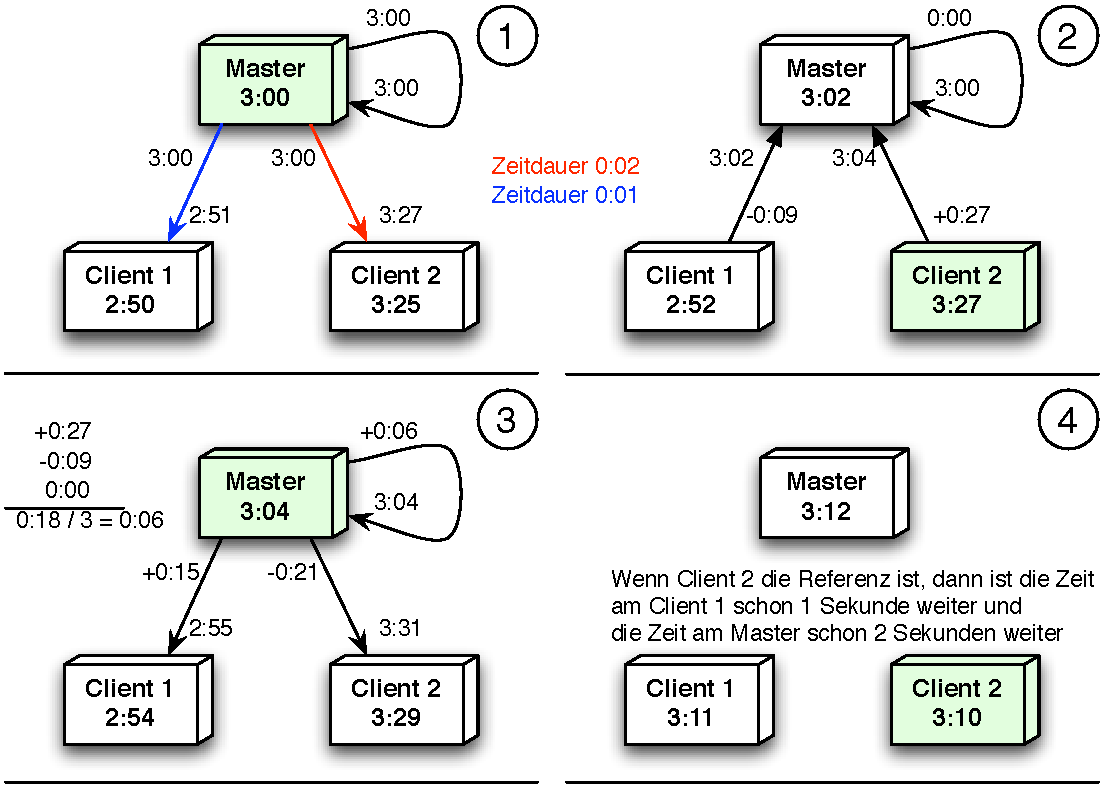
\includegraphics[bb=0bp 0bp 19cm 14cm,clip,scale=0.7]{design_dev/synchronization/berkeley}

\caption{\label{fig:clock_berkeley}Beispiel f�r Berkeley-Algorithmus}

\end{figure}


\selectlanguage{austrian}%

\subsection{Globaler Status}

Nachdem Einigkeit �ber eine gemeinsame Zeitbasis erzielt worden ist,
ist es oft wichtig den \emph{globalen Zustand} einer verteilten Anwendung
zu wissen.

Der globale Status setzt sich aus dem lokalen Zustand aller Prozesse
gemeinsam mit den Nachrichten zusammen, die gerade �bertragen werden.

Aus diesem globalen Status kann z.B. gefolgert werden, ob sich das
System in einem Deadlock befindet.


\subsection{Wechselseitiger Ausschluss}

Es soll der verteilte Zugriff auf eine Ressource geregelt werden.
Dazu gibt es zumindest drei Algorithmen:


\minisec{Zentralisierter Algorithmus}

Es wird die selbe Vorgehensweise herangezogen, die auch im nicht verteilten
System gew�hlt wird. Dazu wird ein zentraler Koordinator bestimmt,
der von allen Einheiten befragt wird und z.B. genau einer den Zugriff
auf die Ressource gestattet. Verl�sst derjenige Prozess wieder den
kritischen Abschnitt meldet er dies ebenfalls dem Koordinator.

Im speziellen funktioniert der \emph{zentralisierter Algorithmus}
folgenderma�en:
\begin{enumerate}
\item Prozess 1 stellt eine Anforderung, um den Zugriff auf eine Ressource
durchf�hren zu k�nnen. 
\item Der Koordinator sendet eine OK-Antwort zur�ck (Erteilung) und somit
kann Prozess 1 in den kritischen Abschnitt eintreten. 
\item In der Zwischenzeit will auch Prozess 2 in den kritischen Abschnitt
eintreten und sendet ebenfalls eine Anfrage an den Koordinator. Dieser
stellt die Anfrage in eine Queue und sendet vorerst keine Antwort
an Prozess 2. 
\item Prozess 1 hat den kritischen Abschnitt verlassen und sendet eine Freigabenachricht
an den Koordinator. 
\item Darauf kann der Koordinator eine OK-Nachricht an Prozess 2 senden. 
\end{enumerate}
Zu sehen ist dieser Ablauf in Abbildung \vref{fig:sync_central}.

Die Vorteile liegen
\begin{itemize}
\item in der einfachen Implementierung: es sind nur drei Nachrichten (Anforderung,
Erteilung, Freigabe) notwendig. 
\item im fairen Behandeln der Anfragen, die genau im Eintreffen der Anforderungen
abgearbeitet werden. Jeder Prozess kommt einmal an die Reihe; es kommt
nicht vor, dass einer endlos warten muss. 
\end{itemize}
Speziell bei dieser M�glichkeit, treten die Probleme auf, die auch
bei zentralisierten Verfahren auftreten:
\begin{itemize}
\item Der Koordinator ist ein zentraler Ausfallpunkt: Wenn dieser ausf�llt,
dann f�llt m�glicherweise das gesamte System aus. 
\item Ein ausgefallener Koordinator kann nicht erkannt werden, wenn dieser
nach Annahme einer Anforderung ausf�llt. Da das Nichtempfangen einer
Freigabe nicht unterschieden werden kann von einem eventuellen Ausfall
des Koordinators. 
\item Der Koordinator kann sich als Leistungsengpass herausstellen und die
Skalierbarkeit begrenzen. 
\item Wenn es keinen dedizierten Koordinator gibt, muss einer gew�hlt werden
(Wahlalgorithmen). 
\end{itemize}
\selectlanguage{ngerman}%
%
\begin{figure}
\centering

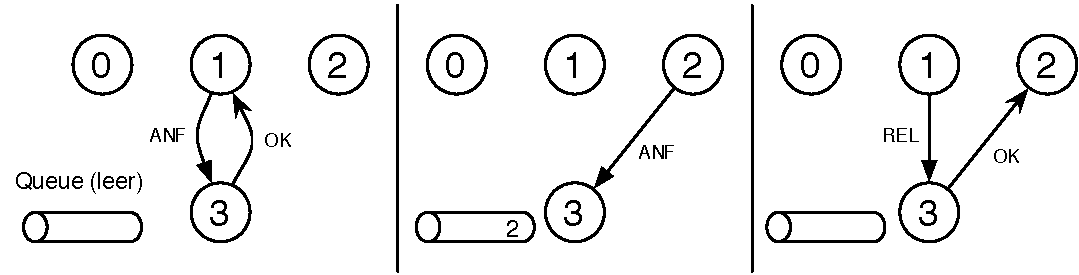
\includegraphics[bb=0bp 0bp 19cm 5cm,clip,scale=0.85]{design_dev/synchronization/sync_central}

\caption{\label{fig:sync_central}Beispiel f�r zentralisierten Algorithmus}

\end{figure}


\selectlanguage{austrian}%

\minisec{Verteilter Algorithmus}

Der \emph{verteilte Algorithmus} funktioniert folgenderma�en:

Ein Prozess, der in den kritischen Bereich eintreten will, erzeugt
eine Anforderungsnachricht, die seine Prozessnummer und die aktuelle
Zeit enth�lt. Diese Nachricht sendet er an alle Prozesse (auch an
sich selbst).

Dies kann entwender durch einzelnes Versenden an alle Prozesse oder
durch Multicasting erfolgen. Wichtig ist, dass die Kommunikation zuverl�ssig
ist, d.h., dass jede Nachricht best�tigt wird.

Erh�lt ein Prozess eine Anforderungsnachricht, ist seine Reaktion
von seinem Status bzgl. dem kritischen Abschnitt abh�ngig: 
\begin{itemize}
\item Befindet sich der Empf�nger nicht im kritischen Bereich und will diesen
auch nicht betreten, dann sendet er eine OK-Nachricht an den Sender
zur�ck. 
\item Befindet sich der Empf�nger im kritischen Bereich, antwortet er nicht.
Stattdessen stellt er die Anforderung in eine Queue. 
\item Will der Empf�nger in den kritischen Bereich eintreten, hat dies aber
noch nicht gemacht, dann vergleicht er den Zeitstempel der eingehenden
Nachricht mit dem der Nachricht, die er selbst versendet hat. Der
niedrigere Zeitstempel gewinnt: Hat die eingehende Nachricht einen
niedrigeren Zeitstempel, dann sendet er eine OK-Nachricht zur�ck.


Hat seine eigene Nachricht einen kleineren Zeitstempel, stellt der
Empf�nger die eingehende Anforderung in die Warteschlange und sendet
nichts. 

\end{itemize}
Hat ein Prozess OK-Nachrichten von allen Prozessen erhalten, dann
kann er in den kritischen Bereich eintreten.

Wird der kritische Bereich verlassen, dann sendet der Prozess OK-Nachrichten
an alle Prozesse in seiner Warteschlange und l�scht sie aus dieser.

In Abbildung \vref{fig:sync_distributed} ist ein Beispiel f�r den
Ablauf einer Synchronisation mittels verteilten Algorithmus zu sehen.

\selectlanguage{ngerman}%
%
\begin{figure}
\centering

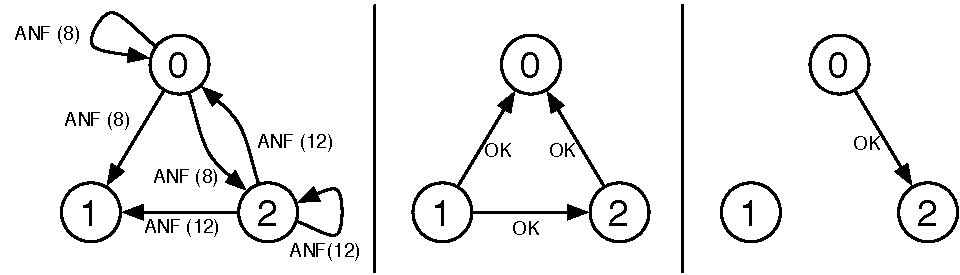
\includegraphics[bb=0bp 0bp 165mm 5cm,clip,scale=0.85]{design_dev/synchronization/sync_distributed}

\caption{\label{fig:sync_distributed}Beispiel f�r verteilten Algorithmus}

\end{figure}


\selectlanguage{austrian}%
Dieser Algorithmus hat jedoch einige gravierende Nachteile: 
\begin{itemize}
\item Anstatt einem Ausfallpunkt gibt es jetzt n Ausfallpunkte. 
\item Bei Einzelversendungen der Anforderungsnachrichten muss jeder Prozess
eine Liste der Gruppenmitglieder verwalten. 
\item Die Skalierbarkeit hat sich auch nicht verbessert, da jetzt alle Prozesse
beteiligt sind und jeder eine Funktion �hnlich dem eines Koordinators
�bernimmt. 
\item Der Algorithmus ist aufw�ndiger und langsamer. 
\end{itemize}

\minisec{Token-Ring-Algorithmus}

Beim \emph{Token-Ring-Algorithmus} werden alle Prozess sind in einem
logischen Ring angeordnet. Jeder muss wissen welcher sein Nachfolger
ist. Es kreist ein Token im Ring. Ist ein Prozess im Besitz des Tokens,
dann kann er in den kritischen Abschnitt eintreten. Nach Verlassen
des kritischen Abschnittes wird das Token weitergegeben. Will kein
Prozess in den kritischen Abschnitt eintreten, kreist das Token mit
hoher Geschwindigkeit im Kreis.

Nachteile: 
\begin{itemize}
\item Es kann auch hier ein Prozess abst�rzen. Dies kann jedoch erkannt
werden, wenn jede Token�bergabe best�tigt werden muss. Wird der Empfang
nicht best�tigt, dann muss dieser Prozess aus dem Ring entfernt werden.
D.h.~bei der �bergabe muss der Vorg�nger den toten Prozess aus dem
Ring herausnehmen und das Token an den �bern�chsten Prozess weitergeben.
D.h.~aber, dass jeder Prozess den gesamten aktuellen Ring kennen
muss! 
\item Es kann ein Token verloren gehen. In diesem Fall muss es neu erzeugt
werden, aber es ist nicht leicht zu erkennen, dass ein Token verloren
gegangen ist. 
\end{itemize}

\minisec{Zusammenfassung}

Es kann gesagt werden, dass der zentrale Algorithmus trotz dessen
gravierenden Nachteile der effizienteste und einfachste Algorithmus
ist.


\subsection{Verteilte Transaktionen}

Prinzipiell: Verteilte Transaktionen weisen �hnliche Charakteristiken
wie ihre nicht verteilten Pendants auf, jedoch treten \emph{zus�tzlich}
die schon besprochenen Probleme auf, die man mit �hnlichen Mechanismen
l�sen kann.\selectlanguage{austrian}



%% 
\chapter{Kommunikation}


\section{TCP/IP Programmierung in Java}


\subsection{Allgemeine Aspekte}


\minisec{IP Adresse in Java}

Die Klasse java.net.InetAddress (abstrakte Basisklasse) stellt eine
Repr�sentierung einer IPv4 bzw.~IPv6 Adresse dar, die die folgenden
Methoden aufweist: 
\begin{itemize}
\item public static InetAddress getByName(String host) 
\item public static InetAddress getLocalHost() 
\item public String getHostName() 
\item public byte{[}{]} getAddress() 
\item public boolean isReachable(int timeout) throws IOException // testet,
ob Rechner innerhalb angegebener Zeit erreichbar ist (mittel ICMP
Echo Request oder TCP Verbingung zu Port 7 (Echo). 
\end{itemize}
Beispiel eines Code-Fragmentes f�r ein `nslookup', `host' oder `dig'-artiges
Programm:


\begin{lstlisting}
try {
  InetAddress address;
  address = InetAddress.getByName("www.htlwrn.ac.at"); 
  System.out.println(address);
} catch (java.net.UnknownHostException e) {
  e.printStackTrace();
}
\end{lstlisting}


Das folgende Beispiel gibt die lokale IP Adresse aus: 


\begin{lstlisting}
import java.net.InetAddress;

public class LocalIP {
  public static void main(String[] args) {
    try {
      InetAddress a;
      a = InetAddress.getLocalHost();
      System.out.println("localhost: name = " + a.getHostName());
      byte[] addr = a.getAddress();
      System.out.print("localhost: addr= ");

      for (int i = 0; i < addr.length; i++) {
        // addr ist ein byte Array; jeder Wert in -128..+127
        // wir ben�tigen einen ganzzahligen Wert! Alle Werte in Java sind
        // vorzeichenbehaftet im Zweierkomplement gespeichert
        int ub = addr[i] < 0 ? addr[i] + 256 : addr[i];
        System.out.print(ub + "."); 
      }
      System.out.println();  
    } catch (java.net.UnknownHostException e) {
      e.printStackTrace(); // zu Testzwecken
    }
  }
}
\end{lstlisting}



\minisec{URL in Java}

Mit der \verb+java.net.URL+ Klasse kann man auf einfache Art und
Weise Dateien aus dem Internet laden.

Dazu gibt es die folgenden Konstruktoren (die alle die MalformedURLException
werfen k�nnen): 
\begin{itemize}
\item public URL(String url) 
\item public URL(String protocol, String host, String file) 
\item public URL(String protocol, String host, int port, String file) 
\end{itemize}
Folgende Methoden stehen zur Verf�gung: 
\begin{itemize}
\item String getProtocol(), String getHost(), int getPort() 
\item String getPath(), String getQuery(), String getFile() // Path+Query 
\item String getRef() 
\item InputStream openStream() throws IOException 
\item URLConnection openConnection() throws IOExceptione // URLConnection
erlaubt auch ConnectionTimeout und andere Charakteristika einer Verbindung
zu setzen. 
\end{itemize}
Das folgende Programm zeigt die Daten zu einer (mit einer von Java
unterst�tzten Protokoll) URL (http, https, file, jar, ftp sind im
J2SE 5.0 enthalten). Aufzurufen mittels \verb+java WebPageReader http://www.orf.at+:


\begin{lstlisting}
public class WebPageReader {
  public static void main(String[] args) {
    URL u; String line; 
    try {
      u = new URL(args[0]);
      // Stream ... byte
      // Reader/Writer ... char
      BufferedReader br = new BufferedReader (
        new InputStreamReader(u.openStream()));

      while ((line = br.readLine()) != null)
        System.out.println(line);
    } catch (Exception e) {
      e.printStackTrace(); // zu Testzwecken
    }
  }
}
\end{lstlisting}



\subsection{TCP Programmierung}

Die \emph{Berkeley-Sockets} wurden erstmals im Berkeley UNIX im Jahre
1986 implementiert. Sie stellen einerseits ein Konzept dar und bieten
andererseits ein API. Diese Schnittstelle hat sich als \emph{die}
Programmierschnittstelle f�r die Kommunikation (im Internet) etabliert.

Vom Konzept her ist ein Socket ein \emph{Kommunikationsendpunkt},
an dem eine Applikation Daten schreiben kann, die �ber das zugrunde
liegende Netzwerk versendet werden sollen, und von dem eingehende
Daten gelesen werden k�nnen. Sockets kann es sowohl f�r TCP als auch
f�r UDP geben.

Aus der Sicht von TCP/IP besteht solch ein Kommunikationsendpunkt
aus einer Kombination von Protokoll (TCP oder UDP), IP Adresse und
Portnummer und identifiziert als solches eindeutig einen Netzwerkprozess.

Ein Paar von zwei Sockets identifiziert damit \emph{eindeutig} eine
Verbindung bei verbindungsorientierten Protokollen (wie z.B. TCP).


\minisec{Interoperabilit�t}

Eine TCP Verbindung im Internet verbindet in der Regel nicht nur Maschinen
des gleichen Typs, sondern verschiedenste Hardware- und Softwareplattformen
miteinander. Aus diesem Grund ist es, im Sinne der \emph{Interoperabilit�t},
wichtig, sich Gedanken �ber die Darstellung der Daten zu machen. Wie
erw�hnt, stellt der TCP/IP Protokollstack keine Darstellungsschicht
zur Verf�gung.

Probleme treten auf bei: 
\begin{itemize}
\item �bertragung von Zeichendaten. Wie sind diese codiert? ASCII, ISO 8859-1,
ISO-8859-15, EBCDIC oder 16-Bit Zeichens�tze wie in der chinesischen
oder japanischen Sprache verwendet wird (Unicode). 
\item �bertragung von Zahlen 

\begin{itemize}
\item big-endian vs. little-endian 

\begin{itemize}
\item big-endian: erstes Byte enth�lt signifikante Bits (z.B. Java, JPEG,
WAV,...,Intel, Alpha). Weitere Bytes mit steigender Adresse enthalten
die weniger signifikanten Bits. big-endian bedeutet so viel wie {}``big
end first''. Wird auch als \emph{network byte order} bezeichnet! 
\item little-endian: letztes Byte enth�lt signifikante Bits (z.B. BMP, GIF,...,Motorala,
Sparc) 
\end{itemize}
\item signed vs. unsigned 
\item Flie�kommazahlen: IEEE Format oder eigene Formate 
\end{itemize}
\item �bertragung von Objekten 
\end{itemize}
\emph{L�sungsm�glichkeiten}:
\begin{itemize}
\item Schaffung eines properit�ren, bin�ren Austauschformates 
\item Schaffung eines bin�ren offenen Austauschformates, wie z.B. XDR (siehe
Abschnitt \vref{sec:ONC-RPC}) oder CDR (siehe Abschnitt \vref{sec:corba}).
\item Schaffung eines textorientierten Austauschformates, wie z.B. bei Verwendung
von XML-RPC (siehe Abschnitt \vref{sec:XML-RPC}) oder SOAP (siehe
Abschnitt \vref{sec:SOAP}). 
\end{itemize}

\minisec{Socket-Basisoperationen}

Die \emph{Socket-Basisoperationen} sind aufgeschl�sselt nach Client
und Server:
\begin{itemize}
\item Client 

\begin{itemize}
\item Verbinden zu einem entfernten Host 
\item Senden von Daten 
\item Empfangen von Daten 
\item Schlie�en der Verbindung 
\end{itemize}
\item Server 

\begin{itemize}
\item Binden eines Sockets zu einem Port 
\item Warten auf eine Verbindungsanfrage und akzeptieren dieser. 
\item Senden und Empfangen von Daten 
\item Schlie�en einer Verbindung 
\end{itemize}
\end{itemize}

\minisec{Clients in Java}

Die Klasse\texttt{ java.net.Socket} stellt die Client-Seite einer
Socketverbindung dar:

Folgende Konstruktoren gibt es in der Socket-Klasse: 
\begin{itemize}
\item Socket(String host, int port) throws UnknownHostException, IOException 
\item Socket(InetAddress host, int port) throws IOException 
\item Socket(String host, int port, InetAddress localHost, int localPort)
throws IOException // bindet zu spezifizierter lokaler Adresse 
\item Socket(InetAddress host, int port, InetAddress localHost, int localPort)
throws IOException 
\item Socket() // ab JDK 1.4 
\end{itemize}
An public Methoden gibt es:
\begin{itemize}
\item InetAddress getInetAddress(), int getPort() 
\item InetAddress getLocalAddress(), int getLocalPort() 
\item InputStream getInputStream() throws IOException 
\item OutputStream getOutputStream() throws IOException 
\item void connect(SocketAddress endpoint, int timeout) throws IO Exception,
SocketTimeoutException // ab JDK 1.4 
\item synchronized void close() throws IOException 

\begin{itemize}
\item Freigabe aller Netzwerk- und Systemressourcen 
\item wenn gepufferter Outputstream: zuerst schlie�en! 
\item schlie�en des Input- oder des Outputstream schlie�t auch die Netzwerksverbindung! 
\end{itemize}
\item void shutdownOutput() throws SocketException 
\item void shutdownInput() throws SocketException 
\item void setSoTimeout(int) throws SocketException 

\begin{itemize}
\item in Millisekunden nach der eine blockende Leseoperation abbricht (0ms
entspricht kein Abbruch) 
\end{itemize}
\end{itemize}
Folgendes Codefragment demonstriert die Verwendung der Socket-Klasse:


\begin{lstlisting}
try {
  Socket s = new Socket(host, port);
  InputStream is = s.getInputStream();
  OutputStream os = s.getOutputStream();
  // normale Stream Operationen!
} catch (IOException e) {
  e.printStackTrace(); // zu Testzwecken
}
\end{lstlisting}



\minisec{Adresse und Port in Java}

Im Gegensatz zur Klasse \texttt{java.net.InetAddress}, repr�sentiert
die Klasse \texttt{java.net.InetSocketAddress} eine IP Adresse samt
einer zugeh�rigen Port-Nummer und stellt somit alle Informationen
zur Verwendung in der Socket-Verarbeitung dar.

Diese Klasse ist eine Unterklasse der Klasse java.net.SocketAddress,
die in der Signatur der \texttt{connect()} Methode der Klasse Socket
verwendet wird. Auch diese Klasse gibt es erst ab JDK 1.4.

Folgende public Konstruktoren (throws IllegalArgumentException): 
\begin{itemize}
\item InetSocketAddress(int port) 
\item InetSocketAddress(InetAddress ia, int port) 
\item InetSocketAddress(String host, int port) 
\end{itemize}

\minisec{Server in Java}

Die java.net.ServerSocket Klasse stellt somit die Server - Seite einer
Socketverbindung dar.

Folgende Konstruktoren: 
\begin{itemize}
\item public ServerSocket(int port) throws IOException // 0 \ldots{} freier
Port 
\item public ServerSocket(int port, int queueLength) throws IOException 
\item public ServerSocket(int port, int queueLength, InetAddress bindAddress)
throws IOException 
\end{itemize}
Anwendung dieser Klasse um alle belegten Ports am Computer festzustellen:


\begin{lstlisting}
import java.io.*; 
import java.net.*;

public class LocalPortScanner {
  static ServerSocket s;

  public static void main(String[] args) {
    for (int port = 1; port <= 65535; port++) {
      try  s = new ServerSocket(port); 
    } catch (BindException e) {
      System.out.println("port " + port + " in use");
    } catch (IOException e) {
      e.printStackTrace(); // zu Testzwecken
    }
  }
}
\end{lstlisting}


Weitere public Methoden:
\begin{itemize}
\item Socket accept() throws IOException 
\item void close() throws IOException 
\item InetAddress getInetAddress(), int getLocalPort() 
\item void setSoTimeout(int) throws SocketException // Timeout bei accept()! 
\end{itemize}
Gem�� den oben genannten Basisoperationen sieht die Grundstruktur
eines Javaprogrammes mit \texttt{ServerSocket}s folgenderma�en aus:


\begin{lstlisting}
ServerSocket server = new ServerSocket(port); // anlegen und binden
Socket client = server.accept(); // auf Client warten 
server.close(); // ServerSocket kann schon geschlossen werden 
OutputStream out = client.getOutputStream(); 
InputStream in = client.getInputStream();
// tats�chlichen Datenaustausch durchf�hren
client.close(); // Verbindung zum Client schlie�en
\end{lstlisting}



\subsection{UDP Programmierung}


\minisec{java.net.DatagramPacket}

Konstruktoren
\begin{itemize}
\item DatagramPacket(byte{[}{]} buffer, int length) // zum Empfangen von
Paketen; length <= 65535! 
\item DatagramPacket(byte{[}{]} buffer, int length, InetAddress address,
int port) // zum Senden 
\item DatagramPacket(byte{[}{]} buffer, int length, SocketAddress address) 
\end{itemize}
Methoden 
\begin{itemize}
\item InetAddress getAddress(), getPort() 
\item byte{[}{]} getData(), int getLength() 
\item void setAddress(InetAddress address), void setPort(int port) 
\item void setData(byte{[}{]} buffer), void setLength(int length) 
\end{itemize}

\minisec{java.net.DatagramSocket}

Konstruktoren (throws SocketException)
\begin{itemize}
\item DatagramSocket() 
\item DatagramSocket(int port) 
\item DatagramSocket(int port, InetAddress address) // multihomed machines 
\end{itemize}
Public Methoden 
\begin{itemize}
\item void send(DatagramPacket) throws IOException 
\item void receive(DatagramPacket) throws IOException 
\item void close() // alle in receive() $\rightarrow$ SocketException 
\item InetAddress getLocalAddress(), int getLocalPort() 
\item void setSoTimeout(int timeout) throws SocketException // receive! 
\end{itemize}

\minisec{Minibeispiel}


\begin{lstlisting}
// auch wenn der Name "Socket" ist,
// impliziert dies keine Verbindung wie in TCP!
DatagramSocket socket = new DatagramSocket();
DatagramPacket packet = new DatagramPacket(data, data.length);
socket.receive(packet);
socket.close();
\end{lstlisting}



\subsection{Beispiele}

mit TCP und UDP


\minisec{daytime}

Dieses Protokoll fragt die lokale Zeit eines entfernten Servers ab.
Es ist sicher eines der einfachsten Protokolle: Verbindung aufbauen,
Antwort lesen, Verbindung schlie�en.

\textbf{Beschreibung}
\begin{itemize}
\item Server sendet Zeit in der Form einer Zeichenkette (in ASCII) 
\item Beschrieben in RFC 867 
\item TCP Port 13, Verbindung (Socket) �ffnen, Antwort lesen, fertig
\item UDP Port 13, leeres Paket senden, Antwort lesen, fertig
\item Format der Antwort ist nicht spezifiziert, deshalb f�r eine Maschine-Maschine
Kommunikation nicht geeignet. 
\item $\rightarrow$ www.time.gov bzw.~time.nist.gov port 17 
\end{itemize}
\textbf{Beispiel: DaytimeClient mit UDP}


\begin{lstlisting}
DatagramSocket socket = new DatagramSocket();
socket.setSoTimeout(5000); // Timeout f�r Socketoperationen auf 5s
// L�nge 1 Byte!
DatagramPacket packet = new DatagramPacket(new byte[256], 1, host, port);
socket.send(packet);

packet.setLength(packet.getData().length); // Empfangspuffer: 256 Bytes!
socket.receive(packet);
socket.close();

byte[] data = packet.getData();
int length = packet.getLength();
System.out.println(new String(data, 0, length, "latin1")); // oder utf-8...
\end{lstlisting}


\textbf{Beispiel: DaytimeServer mit UDP}


\begin{lstlisting}
DatagramSocket socket = new DatagramSocket(p);
DatagramPacket packet = new DatagramPacket(new byte[1], 1); // 1 Byte!

while (true) {
  socket.receive(packet); 
  System.out.println("Received from:...");
  byte[] outBuffer = new java.util.Date().toString().getBytes("latin1");

  packet.setData(outBuffer); 
  packet.setLength(outBuffer.length); // setze aktuelle L�nge
  socket.send(packet);
}
\end{lstlisting}



\minisec{time}

Das Internet Time Protocol umgeht den Nachteil vom daytime - Protokoll,
das das Format der Zeit nicht spezifiziert indem die Sekunden seit
Mitternacht des 1.1.1900 GMT zur�ckgesendet werden. Au�erdem wird
der Wert bin�r �bertragen (in network byteorder).

\textbf{Beschreibung} 
\begin{itemize}
\item Server sendet Zeit in Form von 4 Byte Integer zur�ck. 
\item RFC 868 
\item TCP, UDP Port 37 
\item TCP: Verbindung �ffnen, Antwort lesen, fertig 
\item UDP: Leeres Datagramm senden, Antwort empfangen, fertig 
\end{itemize}
\textbf{Beispiel in Python}

Zum besseren Verst�ndnis f�r das Socket-API folgt nun ein in Python
programmierter Server f�r das time, da sich das Python-API f�r die
Socketprogrammierung am C API orientiert:


\begin{lstlisting}[language=Python]
import socket, struct, time
PORT = 8037
# Referenzzeit
TIME1970 = 2208988800L # Anzahl Sek. zw. 1.1.1900 bis 1.1.1970

# lege Socket an als:
#   AFINET ... INET Socket (und nicht Unix Sockets)
#   SOCKSTREAM ... TCP (und nicht UDP)
serversock = socket.socket(socket.AF_INET, socket.SOCK_STREAM)

# binde einen Port an den Socket ("" ... localhost)
serversock.bind(("", PORT))

# ab wird auf ankommende Verbindungsanfragen gewartet
# backlog: max. Anzahl der Connections in der Queue ist 3
# d.h. es k�nnen allerdings maximal 3 Verbindungen darauf warten,
# verarbeitet zu werden
serversock.listen(3)

print "Lauschen an Port", PORT

while 1:
    # mit accept werden Verbindungen angenommen
    # clientsock ... Socket zum Client
    # clientaddr ... IP Adresse und Port von Client
    clientsock, clientaddr = serversock.accept()
    print "Verbindung von", clientaddr
    t = int(time.time()) + TIME1970 # time(): Zeit in s seit 1.1.1970

    # packe unsigned int (I) in network-byte-order (!) in einen String
    t = struct.pack("!I", t)

    # nun senden (wir nehmen an, dass 4 Bytes gesendet werden k�nnen)
    clientsock.send(t)
    # und den Client-Socket wieder schlie�en
    clientsock.close()
\end{lstlisting}


Der entsprechende Client dazu:


\begin{lstlisting}
import socket, struct, time, datetime

PORT = 8037
TIME1970 = 2208988800L

sock = socket.socket(socket.AF_INET, socket.SOCK_STREAM)

# zum Server verbinden
sock.connect(("", PORT))

# und nun empfangen (wir nehmen an, dass die 4 Bytes empfangen werden...)
t = sock.recv(4)

# wieder auspacken ([0] ... da unpack ein Tupel zur�ckliefert)
# und Sekunden zw. 1.1.1900 und 1.1.1970 wieder abziehen
t = struct.unpack("!I", t)[0] - TIME1970

# und den Socket wieder schlie�en
sock.close()

# und auf der Konsole ausgeben
# Module datetime: Typ datetime mit Factory Funktion fromtimestamp
print datetime.datetime.fromtimestamp(t)
\end{lstlisting}



\minisec{finger}

Dieses Protokoll fragt die Informationen �ber lokale Benutzer eines
entfernten Servers ab. Es ist ein etwas komplexeres, aber trotzdem
sehr einfaches Protokoll: Verbindung aufbauen, Liste der Benutzernamen
senden, Antwort lesen, Verbindung schlie�en. Die eigentliche Spezifikation
ist doch um einiges umfangreicher, aber das Prinzip ist wie beschrieben.

\textbf{Beschreibung}
\begin{itemize}
\item Client sendet Benutzernamen (optional) und danach $<$CRLF$>$ 
\item Server sendet Informationen zur�ck 
\item Beschrieben in RFC 1288 
\item TCP Port 79, Socket �ffnen, Namen senden, Antwort lesen, fertig 
\item $\rightarrow$ finger Kommando 
\end{itemize}
\textbf{Beispiel: Finger Client}


\begin{lstlisting}
import java.net.*;
import java.io.*;

public class Finger {
  private static Socket sock;
  private static String hostname = "localhost";
  private static String line = "";

  public static void main(String[] args) {
    try {
      sock = new Socket(hostname, 10079);
      OutputStreamWriter wr = new OutputStreamWriter(
        sock.getOutputStream());
      if (args.length > 0) {
        wr.write(args[0]);
      }
      wr.write("");
      wr.flush();
      // charset angeben, ansonsten default charset des Systems!
      BufferedReader br = new BufferedReader(
        new InputStreamReader(sock.getInputStream(), "US-ASCII"));

      String line;
      while ((line = br.readLine()) != null)
        System.out.println(line);  
    }
    catch (UnknownHostException e) { e.printStackTrace(); }
    catch (IOException e) { e.printStackTrace(); } // zu Testzwecken
  }
}
\end{lstlisting}



\minisec{echo}

Ein weiteres Protokoll, das analog dem Finger Protokoll funktioniert:
Die Zeichen, die der Client an den Server sendet, sendet dieser als
Antwort wieder zur�ck.

Als weitere Ausbaustufe wird das Beispiel auch als Server entwickelt
(in einer Single-Threaded Version).

\textbf{Beispiel: EchoClient mit TCP}


\begin{lstlisting}
public class EchoClientTCP {
  public static void main(String[] args) throws IOException {
    String host = "localhost";
    int port = 9999;
    Socket sock;
    InputStream in;
    OutputStream out;

    sock = new Socket();
    sock.setSoTimeout(4000); // 4s f�r read()
    try {
      // 2s time-out 
      sock.connect(new InetSocketAddress(host, port), 2000);
    } catch (IOException e) {
      System.out.println("EchoClient: Connection refused");
      System.exit(1);
    }
    in = sock.getInputStream();
    out = sock.getOutputStream();
    System.out.println("Socket port: " + sock.getPort());

    // es wird keine Exception abgefangen...
    int c; // read liefert int!
    while ((c = System.in.read()) != -1) {
      out.write(c);
      System.out.write(in.read());
    }
  }
}
\end{lstlisting}


\textbf{Beispiel: EchoServerST mit TCP}

Ger�st f�r einen Single-Threaded Echo-Server:


\begin{lstlisting}
import java.io.*;
import java.net.*;

public class EchoServerST {
  static int port = 9999;

  public static void main(String[] args) throws IOException {
    ServerSocket server = new ServerSocket(port);
    Socket client = server.accept();
    client.setSoTimeout(10000); // max. 10s warten!
    server.close();
    OutputStream out = client.getOutputStream();
    InputStream in = client.getInputStream();
    int x;

    try {
      while ((x = in.read()) > -1)
        out.write(x);
    } catch (InterruptedIOException e) {
      client.close();
    }
  }
}
\end{lstlisting}



\section{Nachrichtenorientierte Kommunikation}

Das charakteristische Merkmal der nachrichtenorientierten Kommunikation
ist, dass die Kommunikation durch Versenden von Nachrichten stattfindet.

Im Prinzip l�sst sich jede Kommunikation auf diese Abstraktionsebene
zur�ckf�hren. Genauso wie sich jede Programmierung letztendlich auf
die Maschinensprachen- bzw. Assemblerprogrammierung zur�ckf�hren l�sst.


\subsection{Typen von Nachrichten\label{sec:message_types}}

Prinzipiell kann zwischen \emph{zwei verschiedenen Arten} der Nachrichten�bermittlung
unterschieden werden: 
\begin{description}
\item [{synchron}] Operation beginnt nur, wenn Sender die Nachricht initiiert
hat und der Empf�nger bereit ist die Nachricht zu empfangen. Diese
Art kann noch mit einem Timeout versehen werden. D.h.~es handelt
sich bei einer Operation zum synchronen Nachrichtenaustauch um einen
blockenden Aufruf. 
\item [{asynchron}] Sender initiert das Senden der Nachricht, unabh�ngig
ob Empf�nger bereit ist oder nicht. Prinzipiell handelt es sich bei
einer Operation zum asynchronen Nachrichtenaustausch um einen nicht
blockenden Aufruf. Da die Nachrichten u.U. in einem Puffer zwischengespeichert
werden wird m�glicherweise trotzdem blockiert, damit es zu keinem
Puffer�berlauf kommt.
\end{description}
Untersucht man die Semantik der Interprozesskommunikation genauer,
kann zwischen drei Arten unterschieden werden: 
\begin{description}
\item [{no-wait~send}] Der Sendeprozess wartet lediglich bis die Nachricht
im Transportsystem zum Absenden bereitgestellt ist (siehe Abbildung
\vref{fig:no_wait_send}).
\item [{synchronization~send}] Der Sendeprozess wartet bis die Nachricht
vom Empfangsprozess entgegengenommen worden ist (siehe Abbildung \vref{fig:synchronization_send}).
\item [{remote-invocation~send}] Der Sendeprozess wartet bis die Nachricht
vom Empfangsprozess verarbeitet und beantwortet worden ist (siehe
Abbildung \vref{fig:remote_invocation_send}).
\end{description}
%
\begin{figure}
\centering

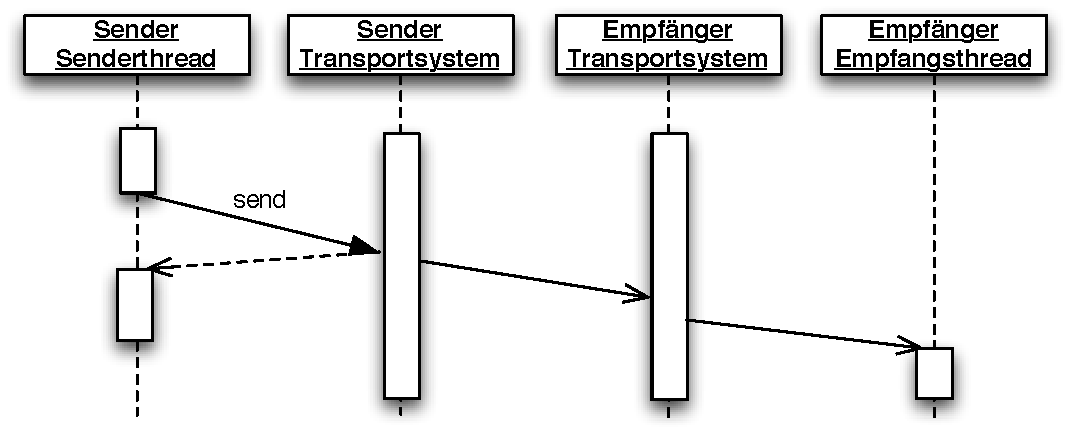
\includegraphics[bb=0bp 0bp 19cm 75mm,clip,scale=0.7]{design_dev/communication/no-wait_send}

\caption{\label{fig:no_wait_send}no-wait send}

\end{figure}


%
\begin{figure}
\centering

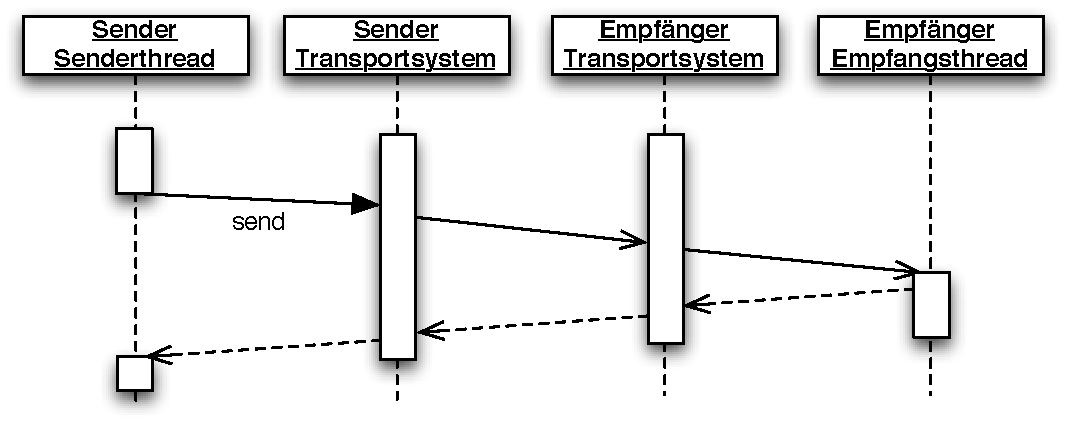
\includegraphics[bb=0bp 0bp 19cm 75mm,clip,scale=0.7]{design_dev/communication/synchronization_send}

\caption{\label{fig:synchronization_send}synchronization send}

\end{figure}


%
\begin{figure}
\centering

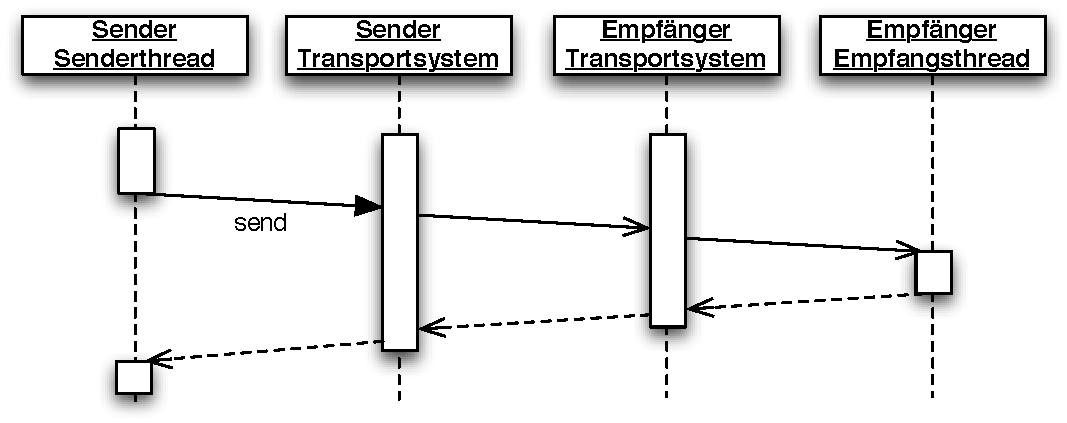
\includegraphics[bb=0bp 0bp 19cm 75mm,clip,scale=0.7]{design_dev/communication/remote-invocation_send}

\caption{\label{fig:remote_invocation_send}remote-invocation send}

\end{figure}


Seitens der Implementierung kann man folgende IPC Varianten erkennen: 
\begin{description}
\item [{non-blocking~send}] $\rightarrow$ no-wait send 
\item [{blocking~send}] Der Sendeprozess wartet bis die Nachricht den
Rechner verlassen hat, d.h.~ins Netz eingespeist worden ist. 
\item [{reliable-blocking~send}] Der Sendeprozess wartet bis die Nachricht
beim Empfangsrechner eingetroffen ist bzw.~von dem Betriebssystem
angenommen worden ist. 
\item [{explicit-blocking~send}] $\rightarrow$ synchronization send 
\item [{request/reply}] $\rightarrow$ remote-invocation send 
\end{description}

\subsection{Transiente Kommunikation}

Die \emph{transiente Kommunikation} als Form der nachrichtenorientierten
Kommunikation ist dadurch gekennzeichnet, dass beide Kommunikationspartner
online sein m�ssen und die Nachrichten vom unterliegenden Kommunikationssystem
nur solange gespeichert werden, wie die sendende und die empfangene
Applikation ausgef�hrt wird. D.h.~auf diesem niedrigen Abstraktionsniveau
ist diese Kommunikation als synchron zu betrachten.

Normalerweise unterst�tzen alle Kommunikationsdienste auf der Transportebene
nur die transiente Kommunikation. Diese Art entspricht der Kommunikation
wie in den obigen Beispielen und wird mittels Sockets oder Datagrams
realisiert.


\subsection{Persistente Kommunikation}

Bei einer \emph{persistenten Kommunikation} wird eine Nachricht vom
Kommunikationssystem solange gespeichert, wie es dauert, sie an den
Empf�nger auszuliefern.

Im Sinne der Einteilung der Typen der Nachrichten sind auch hier sowohl
synchrone als auch asynchrone Nachrichten m�glich.

Motivation: 
\begin{itemize}
\item Was ist, wenn der Server offline ist? 
\item Was ist, wenn es keine Netzwerkroute zum Server gibt? 
\end{itemize}
Ein konkrete Implementierung der persistenten Kommunikation ist unter
dem Titel `Message Oriented Middleware' bekannt.


\section{Message Oriented Middleware\label{sec:MOM}}

Bei der `Message Oriented Middleware' handelt es sich um eine Abstraktion
der persistenten nachrichtenorientierten Kommunikation, die eine Programmierung
mit Nachrichten auf einer h�heren Abstraktionsebene zur Verf�gung
stellt.

Unter \emph{Message Oriented Middleware} (MOM) versteht man 
\begin{itemize}
\item eine Softwareinfrastruktur, die 
\item durch asynchrone Verbindungen charakterisiert ist und 
\item mehrere Systeme durch 
\item Nachrichten miteinander verbindet. 
\end{itemize}
MOM Systeme unterst�tzen persisitente Kommunikation und lassen sich
folgenderma�en \emph{charakterisieren}: 
\begin{itemize}
\item Abstraktion der Schnittstellen erfolgt mittels Datenbeschreibungen:
Der zugrundeliegende Mechanismus sieht den einfachen Austausch durch
Nachrichten vor. 
\item Abstraktion der unterliegenden Transportkommunikation: Die Anwendung
muss nicht wissen welche Transportprotokolle verwendet werden. D.h.
als zugrundeliegendes Transportprotokoll kann HTTP, SMTP, FTP,...
verwendet werden. 
\item Lose gekoppelte (asynchrone) Kommunikation: Es ist nicht erforderlich,
dass der Empf�nger ausgef�hrt wird, wenn eine Nachricht gesendet wird.
Analog dazu ist es nicht erforderlich, dass der Sender ausgef�hrt
wird, wenn seine Nachricht vom Empf�nger entgegengenommen wird. 
\item Mehrere Kommunikationsmodelle sind m�glich (siehe weiter unten). 
\item Bei der Kommunikation sind viele Knoten beteiligt. 
\item Au�erdem stellt die MOM-Software meistens Transaktionen (Auslieferung
mehrer Nachrichten als atomare Aktion), Persistenz und Quality-of-Service
(QoS) Dienste (z.B. Priorit�t oder Time-to-Live) zur Verf�gung. 
\end{itemize}
\textbf{Beispiel (fiktiv)}

Alle Kassenautomaten der �BB sind vernetzt. Jeder Kassenautomat ist
direkt mit genau einem Router verbunden, die wiederum untereinander
verbunden sind. Der Tarifrechner der �BB ist ebenfalls an das Netzwerk
angeschlossen und mit einem Router verbunden.

Die Tarife m�ssen (wieder einmal) um 10\% erh�ht werden. Dazu sendet
(asynchron) der Tarifrechner eine Nachricht (die an alle Kassenautomaten
adressiert ist) an seinen Router. Dieser speichert diese Nachricht
persistent ab und sendet sie an alle Router weiter, die notwendig
sind, um alle Kassen zu verst�ndigen. Ist eine Kasse nicht in Betrieb
(z.B. auf Grund einer St�rung; soll schon vorgekommen sein), dann
speichert der zugeh�rige Router die Nachricht bis diese ausgeliefert
werden kann.

Derartige Router werden auch Broker genannt und k�nnen auch geclustered
werden, um die Verf�gbarkeit und den Durchsatz zu erh�hen.

Die \emph{zwei wichtigsten Kommunikationsmodelle} im Zusammenhang
mit MOM sind: 
\begin{description}
\item [{Publish/Subscribe}] Es handelt sich um eine one-to-many Kommunikationsart.
Ein Client publiziert Nachrichten zu einem Thema (topic) und andere
Clients k�nnen ein Topic subskribieren. Alle subskribierten Clients
bekommen die Nachrichten, wenn sie sich das n�chste Mal mit dem Broker
verbinden. 
\item [{Point-to-Point}] Die Nachricht wird in eine (Sender-)Queue gestellt
und aus einer (Empf�nger-)Queue sequentiell gelesen. 
\end{description}
Produkte: JMS (Sun), MSMQ (Microsoft), MQSeries (IBM), SwiftMQ (IIT
Software),...


\section{Entfernte Prozeduraufrufe}

Nachrichtenorientierte Kommunikation wie vorhergehend besprochen,
verbergen den unterliegenden Kommunikationscharakter nicht vollst�ndig
im Sinne der Zugriffstransparenz (d.h.~dass Nachrichten versendet
werden).

Deshalb ist man dazu �bergegangen die Semantik der lokalen Funktionsaufrufe
auf \emph{entfernte Funktionsaufrufe} (Remote Procedure Call, RPC)
auszudehnen.

Die Funktionsweise derartiger entfernter Funktionsaufrufe sieht folgenderma�en
aus: Wenn ein Prozess auf Maschine A eine Prozedur auf Maschine B
aufruft, wird der ausf�hrende Prozess auf A unterbrochen, die Ausf�hrung
der entfernten Prozedur auf B findet statt und danach wird der Prozess
auf A fortgef�hrt. Alle notwendigen Parameter, R�ckgabewerte und auch
eventuelle Exception werden transparent �bertragen.

Diese Eleganz hat einige Probleme, die gel�st werden m�ssen: 
\begin{itemize}
\item Was passiert, wenn es sich um unterschiedliche Plattformen handelt,
die die zugrundeliegenden Datentypen unterschiedlich repr�sentieren?


Eine 16 Bit ganze Zahl verschieden abgespeichert werden kann ($\rightarrow$
Interoperabilit�t, Darstellungsschicht). Aber auch die Abspeicherung
in verschiedenen Dateiformaten variert.

Aus diesen Gr�nden gibt es zwei M�glichkeiten wie Daten �ber das Netzwerk
�bertragen werden k�nnen: 
\begin{itemize}
\item Entweder werden die Daten in ein maschinenunabh�ngiges Format transformiert
in das beide Kommunikationspartner ihre Daten wandeln und wieder zur�ckwandeln
(Overhead, wenn beide Partner, die gleiche Darstellung verwenden,
die jedoch von der maschinenunabh�ngigen Darstellung differiert):
single-canonical format. 
\item Oder der Empf�nger muss sich um eine evtl. notwendige Konvertierung
k�mmern. Dazu spezifiziert der Sender den Datentyp aus einer Liste
von vorgegebenen Datentypen: receiver-makes-it-right. 
\end{itemize}
Probleme wie little-endian vs.~big-endian treten z.B. \emph{auch}
bei der �bertragung von 16-bit Unicodezeichen auf.

Ein weiteres Beispiel: Wie ist zu verfahren, wenn eine Architektur
keine unsigned Zahlen kennt, diese aber �ber das Netzwerk empf�ngt
(z.B. Java kennt keine unsigned Zahlen)? 

\item Wie wird mit Parametern umgegangen, die mittels call-by-reference
�bergeben werden? Wie werden Objekte mit call-by-value �bertragen
(zwischen verschiedenen Plattformen)?
\item Wie wird mit auftretenden Exceptions verfahren?
\item Wie wird verfahren, wenn die eine oder die andere Maschine abst�rzt? 
\end{itemize}
Um diese Probleme zu l�sen und die Transparenz zu gew�hrleisten wird
folgender Ansatz gew�hlt: Es werden \emph{Client- und Server Stubs}
generiert. Der Client Stub stellt eine Schnittstelle der entfernten
Funktion zur Verf�gung, wandelt alle Parameter in die Datenrepr�sentierung
und spricht �ber ein Protokoll mit dem Server Stub. Der Server Stub
wandelt die Daten und ruft die lokale Funktion am Server auf. Der
R�ckgabewert geht den umgekehrten Weg wieder zur�ck.

Der Server Stub wird auch oft als Skeleton bezeichnet.

D.h. man ben�tigt die folgenden 3 Komponenten, um entfernte Prozeduraufrufe
durch f�hren zu k�nnen:
\begin{enumerate}
\item Maschinen-unabh�ngige Datenrepr�sentierung samt der notwendigen Runtime
Software. 
\item Ein Protokoll, das die Stubs verwenden, um miteinander zu kommunizieren. 
\item Einen Protokoll-Compiler, der aus einer Funktionsdefinition die Stubs
generiert. 
\end{enumerate}
Schaut man sich die Fernaufrufe etwas genauer an, dann erkennt man
wieder, dass auch hier verschiedene Varianten m�glich sind: 
\begin{description}
\item [{synchrone}] Funktionsaufrufe haben die Semantik `remote-invocation
send' 
\item [{synchrone}] Prozeduraufrufe haben die Semantik `synchronization
send' 
\item [{asynchrone}] Prozeduraufrufe haben die Semantik `no-wait send' 
\item [{asynchrone}] Funktionsaufrufe haben ebenfalls die Semantik `no-wait
send'. Um auf den R�ckgabewert zuzugreifen gibt es zwei M�glichkeiten: 

\begin{description}
\item [{polling}] Modell Es wird ein Objekt beim Aufruf mitzugeben. In
diesem Objekt wird das Resultat zu einem sp�teren Zeitpunkt eingetragen.
Dieses Objekt kann auf das Resultat abgefragt werden (blockend oder
pollend). 
\item [{callback}] Modell Beim Aufruf wird eine Callback-Funktion mitgegeben.
Diese wird dann aufgerufen, wenn das Resultat eingelangt ist. 
\end{description}
\end{description}
Funktionsaufrufe (liefert einen Wert) und Prozeduraufrufe (liefert
keinen Wert) stehen hier auch f�r das objektorientierte Gegenst�ck
(der Methode). D.h.~Methoden werden als objektgebundene Funktionen
gesehen (was sie letzlich auch sind).


\subsection{ONC RPC\label{sec:ONC-RPC}}

ONC (Open Network Computing) RPC wurde von Sun spezifiziert und implementiert
und war lange Zeit ein defacto Standard (1995 als RFC 1831 standardisiert)
f�r die Kommunikation zwischen verschiedenen Rechner (auch zwischen
verschiedenartigen Rechnerarchitekturen und Betriebssystemen) basierend
auf der Semantik von entfernten Prozeduraufrufen (und wird heute noch
z.B. f�r das Network File System - NFS verwendet).

ONC RPC kann als unterliegendes Transportprotokoll sowohl TCP als
auch UDP verwenden.

Das Ziel dieser Technologie war es, eine einfache synchrone Kommunikation
aufzubauen, die transparent den Zugriff auf die entfernte Maschine
erm�glicht.

Im Sun RPC Modell wird eine single-canonical format Datenrepr�sentierung
in einem bin�ren Format verwendet. Diese wird XDR (eXternal Data Representation)
genannt.

Dazu m�ssen die Funktionsdeklarationen in einer eigenen Interface
Definition Language (IDL) festgeschrieben, die in diesem Fall RPCL
(RPC Language) genannt wird. Diese RPCL ist eine C �hnliche Sprache.
Aus dieser RPCL generiert ein Protokollcompiler (RPCGEN genannt) die
Stubs.

In gewisser Weise kann auch das ONC RPC auf das OSI Modell abgebildet
werden:
\begin{itemize}
\item Schicht 7 (Anwendung) 
\item Schicht 6 (Darstellung): XDR 
\item Schicht 5 (Session): RPC 
\item Schicht 4 (Transport): TCP oder UDP 
\item Schicht 3 (Vermittlung): IP 
\end{itemize}
Eine Frage bleibt derzeit noch offen: Wie findet ein Client seinen
entfernte Funktion? 
\begin{itemize}
\item Ein Serverprozess wird auf einer Maschine gestartet und lauscht an
einem Port auf einkommende Funktionsaufrufe. Wie kann der Client die
Portnummer erfahren? 
\item Jedes Programm muss sich, aus einem gewissen Bereich, eine eindeutige
Programmnummer w�hlen, weiters eine Versionsnummer und f�r jede Funktion,
die �ber das Netzwerk angeboten wird, eine Funktionsnummer. Diese
Angaben werden bei einem speziellen Server (dem portmapper) registriert.
Dieser Server lauscht an einem definierten Port (111). 
\item Ein Client richtet eine Anfrage bzgl.~eines Programmes in einer bestimmten
Version an den Portmapper und erh�lt von diesem die Portnummer, unter
der der Serverprozess l�uft mitgeteilt, sodass der Client direkt eine
Verbindung aufnehmen kann. 
\end{itemize}
Es handelt sich um ein allgemeines Prinzip, das im Abschnitt `Serverseitiges
Programmieren' nochmals behandelt wird.

Zus�tzlich sind im ONC-RPC noch einige Erweiterungen, wie z.B. eine
einfache Authentifierung enthalten. Trotzdem ist dieses Technologie
weitgehend durch DCE-RPCs (Distributed Computing Environment von der
Open Software Foundation, OSF) und objektbasierte und objektorientierte
RPCs verdr�ngt worden.


\section{Entfernte Methodenaufrufe}

Mit der Objektorientierung sind zus�tzlich noch weitere Anforderungen
an die Systeme zum \emph{Aufruf von entfernten Methoden} aufgetreten:
\begin{itemize}
\item Serialisierung/Deserialisierung der Objekte (marshalling). Da es sich
um Objekte handelt, die Instanzen von Klassen sind, muss entweder
die Klasse am Client vorhanden sein, oder diese muss dynamisch zur
Laufzeit geladen (�bertragen) werden. 
\item R�ck�bermittlung der Exceptions 
\item Distributed Garbage Collection 
\item Activation: Es ist nicht immer sinnvoll oder gar machbar, dass alle
Serverimplementierungen die gesamte Zeit laufen zu lassen. Folglich
sollte es eine M�glichkeit geben Serverobjekte zur Laufzeit zu aktivieren. 
\item Versionsmanagement (der Programme, der Objekte) 
\end{itemize}
Diese und �hnliche Aspekte werden von objektbasierten verteilten System
wie CORBA, DCOM oder Java-RMI abgedeckt.

Der folgende Abschnitt behandelt im speziellen die RMI Technologie,
die in der J2SE und der J2EE enthalten ist.


\subsection{RMI}

\emph{Remote Method Invocation} (RMI) ist einerseits ein �berbegriff
f�r eine Objekt-zu-Objekt Kommunikation. Andererseits wird damit eine
spezielle Technologie in der Java Plattform bezeichnet.

In RMI wird der Server Stub als Skeleton bezeichnet. Weiters gibt
es einen 'Remote Reference Layer', der f�r die Verwaltung der entfernten
Referenzen zust�ndig und auch eine 'Distributed Garbage Collection'
durchf�hrt.

Folgende �bersicht stellt wieder eine M�glichkeit zur Einordnung in
das OSI Modell vor: 
\begin{itemize}
\item Schicht 7 (Anwendung): Client, der eine Methode aufruft und entferntes
Objekt, das eine Methode zur Verf�gung stellt. Achtung: aus dieser
Sicht handelt es sich nicht um den Anwenderprozess.
\item Schicht 6 (Darstellung): Stub bzw. Skeleton 
\item Schicht 5 (Session): Remote Reference Layer 
\item Schicht 4 (Transport): JRMP (Java Remote Method Protocol) �ber TCP;
Gibt es Firewallprobleme, dann ist es auch m�glich RMI �ber IIOP (Internet
Inter-ORB-Protocol) zu betreiben. 
\item Schicht 3 (Vermittlung): IP 
\end{itemize}
Vorgehensweise zum Entwickeln von Applikationen mit RMI: 
\begin{enumerate}
\item Ein Remote Interface definieren, das die Methoden enth�lt, die �ber
entfernt zur Verf�gung gestellt werden k�nnen.


Dazu muss dieses Interface public sein, von java.rmi.Remote abgeleitet
werden und alle Methoden m�ssen die java.rmi.RemoteException in ihrer
throws Klausel enthalten. Zus�tzlich kann nat�rlich jede Methode eigene
Exceptions definieren. 

\item Eine Klasse schreiben, die dieses Remote Interface implementiert.


Diese Klasse muss von java.rmi.server.UnicastRemoteObject (oder java.rmi.activation.Activatable)
abgeleitet werden, damit es als Serverobjekt auftreten kann.

Wenn die Klasse jedoch schon von einer anderen Klasse abgeleitet ist,
besteht die M�glichkeit mittels 'UnicastRemoteObject.exportObject(this)'
im Konstruktor der Klasse dieses zu einem Serverobjekt zu machen. 

\item Danach ist der Client zu schreiben.


Dazu wird eine M�glichkeit ben�tigt, um auf das entfernte Objekt zuzugreifen.
Dazu gibt es prinzipiell zwei M�glichkeiten: 
\begin{itemize}
\item Zugriff �ber einen RMI eigenen Zugriff. 
\item Zugriff �ber das Java Naming and Directory Interface (JNDI), das auch
den Zugriff auf ein LDAP Verzeichnis erlaubt. 
\end{itemize}
\item Im Anschluss sind die Stubs und die Skeletons zu generieren.


Ab JDK 1.2 werden keine Skeletons mehr ben�tigt, da diese Information
jetzt durch Reflection gewonnen werden kann. 

\item Danach ist die Registry zu starten und die Serverobjekte m�ssen registriert
werden.


Dazu muss ein eigenes Programm geschrieben werden, das ein Serverobjekt
anlegt und dieses bei der Registry registriert. Diese Registry ist
au�erdem noch zu starten. Entweder mittels dem Kommandozeilenprogramm
rmiregistry oder mittels der Klasse LocateRegistry.

Beim Starten der Registry ist zu beachten, dass der CLASSPATH schon
richtig gesetzt ist, der alle Stubs .class Dateien enth�lt (oder den
automatischen Download von class Dateien verwenden kann).

Wenn das automatische Laden von class Dateien �ber das Netzwerk gew�nscht
ist, dann muss noch folgendes gemacht werden: 
\begin{itemize}
\item Es muss eine Policy - Datei erstellt werden. 
\item Die Registry muss mit Angabe dieser Policy Datei gestartet werden. 
\item Der Client muss einen SecurityManager instanzieren. 
\end{itemize}
\item Danach kann sowohl der Server als auch der Client gestartet werden. 
\end{enumerate}

\minisec{Beispiel: Berechnung der Potenz}

Zuerst das Interface, der schon bekannten Methode zur Berechnung der
Potenz:


\begin{lstlisting}
import java.rmi.Remote;
import java.rmi.RemoteException;

public interface Power extends Remote {
  public double pow(double x, double y) throws RemoteException;
}
\end{lstlisting}


Und jetzt die Implementierung dieses Interfaces:


\begin{lstlisting}
import java.rmi.RemoteException;
import java.rmi.server.UnicastRemoteObject;

public class SimpleCalculator extends UnicastRemoteObject implements Power {
  public SimpleCalculator() throws RemoteException {
    super();
  }

public double pow(double x, double y) throws RemoteException {
  return Math.pow(x, y);
}
\end{lstlisting}


Und jetzt wird der Clientcode entwickelt:


\begin{lstlisting}
import java.rmi.*;
import java.net.MalformedURLException;

public class Client {
  public static void main(String[] args) {
    if (args.length != 1) {
      System.out.println("usage: Client <hostname>");
      System.exit(1);
    }
    String url = "rmi://" + args[0] + "/SimpleCalculator";
    try {
      Power obj = (Power) Naming.lookup(url);
      double res = obj.pow(2, 3);
      System.out.println("2 ** 3 = " + res);
    } catch (NotBoundException e) {
      System.out.println("/SimpleCalculator nicht in Registry vorhanden");
      System.exit(1);
    } catch (MalformedURLException e) {
      System.out.println("URL fehlerhaft: " + url);
      System.exit(1);
    } catch (RemoteException e) {
      System.out.println("Fehler bei Daten�bertragung" + e.getMessage());
      System.exit(1);
    }
  }
}
\end{lstlisting}


Danach sind die Stubs (und die Skeletons) zu generieren: \verb+$ rmic -v1.2 SimpleCalculator+

Jetzt ist noch in Serverobjekt bei der Registry zu registrieren:


\begin{lstlisting}
import java.rmi.*;
public class Server {
  public static void main(String[] args) {
    try {
      SimpleCalculator obj = new SimpleCalculator();
      Naming.rebind("/SimpleCalculator", obj);
      System.out.println("SimpleCalculator in registry eingetragen!");
    } catch (Exception e) {
      e.printStackTrace();
    }
  }
}
\end{lstlisting}


Um dieses Programm ablaufen zu lassen, muss zuerst die Registry gestartet
werden: \texttt{rmiregistry}. Danach wird der Server und danach die
Clients gestartet.


\section{Stream-orientierte Kommunikation}

Stream-orientierte Kommunikation unterscheidet sich insofern von den
vorhergehenden Kommunikationsarten, dass 
\begin{itemize}
\item nicht abgeschlossene Informationseinheiten ausgetauscht werden und 
\item das Zeitverhalten wesentlich ist. 
\end{itemize}
Beispiel: Die �bertragung eines Audio-Stream, der mit einer Frequenz
von 44100 Hz aufgezeichnet. Um den Originalklang herzustellen, ist
es wesentlich, dass die Samples im Audio-Stream in derselben Reihenfolge
abgespielt und in den Intervallen zu 1/44100 Sekunden abgespielt werden.

Besonders wichtig ist, dass das unterliegende Kommunikationssystem
QoS (Quality of Service, Dienstg�te) Anforderungen erf�llen kann.

Diese sind z.B. Bandbreite, �bertragungsschwierigkeiten, Verz�gerungen
usw. zu nennen.

Noch komplizierter wird es, wenn mehrere Streams zu synchronisieren
sind (z.B. den Audio Kanal zu einer Video�bertragung).


%% 
\chapter{Serverseitiges Programmieren}

Nachdem wir jetzt die Grundlagen der Prozessbehandlung, der Synchronisation
und der Kommunikation kennengelernt haben, k�nnen wir uns die Techniken
der serverseitigen Programmierung genauer ansehen.

Darunter versteht man alle Mechanismen und Methoden, die notwendig
sind, um robuste, performante und skalierbare Server zu \emph{programmieren}.

Es ist extrem schwierig diese Ziele im Kontext von gro�en verteilten
Anwendungen zu erreichen!

Wie k�nnen robuste Server entwickelt werden? 
\begin{itemize}
\item Auswahl einer entsprechenden Technologie 

\begin{itemize}
\item Betriebssystem, z.B. WinXP Server vs. Win98 
\item Middlewaretechnologie 
\item Programmiersprache, z.B.: Java vs. C 
\item Entwurfswerkzeug 
\end{itemize}
\item Entwicklungsprozess (Qualit�tssicherung, Peer reviews, Codegenerierung,...) 
\item Entwurf und Programmierstil 

\begin{itemize}
\item Programmierstil: Verwendung von Exceptions, Fehler�berpr�fungen und
Fehlerbehandlung, Dokumentation, Verwendung von Invarianten,... 
\item Verwendung von funktionierenden L�sungsans�tzen (u.a. Design patterns,
Idioms,...) 
\item Programmiermodell 

\begin{itemize}
\item Wie wird der Server strukturiert? 
\item Wie werden Ressourcen verwaltet? 
\item Werden Threads eingesetzt oder Prozesse? 
\item Oder gibt es event-gesteuerte, kooperative Tasks? 
\item Wird Protokollierung (audit trail) eingesetzt? 
\end{itemize}
\end{itemize}
\end{itemize}
Beispiele von Fragestellungen bzgl. der Performanz und der Skalierbarkeit: 
\begin{itemize}
\item Skaliert die Technologie mit (triviales Beispiel: Benutzerdaten in
Datei vs. in Datenbank)?
\item Werden die Synchronisationsma�nahmen zu einem gro�en Overhead? 
\item K�nnen die Threads auf andere Prozesse oder gar auf verschiedene Computer
verschoben werden? 
\item Wird ein Connection-Pooling zu einer Datenbank eingesetzt? 
\end{itemize}

\section{Allgemeine Serveraspekte}


\subsection{Iterative vs. Nebenl�ufige Server}

Es kann zwischen zwei Arten von Servern unterschieden werden: 
\begin{itemize}
\item \emph{iterativer oder sequentieller Server}: Das Kennzeichen ist,
dass der Server die Anfragen selbst verarbeitet und ggf.~die Antwort
an den Client sendet.


Es ist verst�ndlich, dass solch ein Server nicht lange f�r die Behandlung
einer einzelnen Nachricht ben�tigen darf, da sonst das Antwortzeitverhalten
f�r weitere Anforderungen nicht befriedigend sein wird.

Ein iterativer Server tritt in der Regel entweder auf als: 
\begin{itemize}
\item \emph{blocking Server}: Es werden blockierende Funktionsaufrufe verwendet
(z.B. f�r accept, read, write). In diesem Fall kann er nicht mehr
als eine Verbindung zu einem Client betreiben. 
\item \emph{nonblocking Server}: Es werden keine blockierenden Funktionsaufrufe
verwendet. Dazu gibt es zwei M�glichkeiten: 

\begin{itemize}
\item Es wird polling betrieben. Z.B. wird in Java mittels der \texttt{available()}
Methode der Klasse InputStream in einer Schleife abgefragt, ob Daten
vorhanden sind.


Dies ist nat�rlich keine performante Variante, da aktiv Prozessorzeit
vernichtet wird.

Eine leicht verbesserte Version k�nnte Wartezeiten einf�gen (z.B.
mittes \texttt{Thread.sleep} oder mittels \texttt{setSoTimeout} der
Klasse \texttt{Socket} und Verwendung der blocking \texttt{read} Methode
von Socket).

In Java waren dies bis zur Version 1.4 des JDK die einzigen M�glichkeiten
einen iterativen Server als nonblocking Server zu implementieren. 

\item Die bessere Variante liegt in der Verwendung des select API, das urspr�nglich
im BSD Unix definiert wurde. Das Prinzip ist, dass eine Menge von
Ereignissen registriert werden kann und ein einzelner blockierende
Aufruf (n�mlich select) durchgef�hrt wird, der solange blockiert bis
eines dieses Ereignisse eingetreten ist.


Ein Beispiel ist im Abschnitt \vref{sec:select-based-server} zu finden. 

\end{itemize}
\end{itemize}
\item \emph{nebenl�ufigen Server} (concurrent): Dieser verarbeitet die Anforderungen
nicht selbst, sondern gibt sie an einen separaten Prozess oder Thread
weiter und wartet auf die n�chste Anforderung.


Ein Beispiel ist im Abschnitt \vref{sec:multi-threaded-server} zu
finden. 

\end{itemize}

\subsection{Daemon-Server vs. Super-Server}

Ein weiterer Aspekt ist, wie Clients einen Server kontaktieren. Clients
senden Anforderungen an einen Endpunkt (Port) und jeder Server lauscht
an einem Port. Wie erfahren die Clients mit welchen Port sie sich
verbinden sollen, um einen bestimmten Dienst in Anspruch nehmen zu
k�nnen?

Es gibt einerseits die M�glichkeit, dass einem Dienst ein Port zugewiesen
ist, andererseits ist es f�r viele Dienste nicht notwendig, dass sie
dauerhaft einen zugewiesenen Endpunkt haben. Es ist durchaus m�glich,
dass sie dynamisch einen Port zugewiesen bekommen. Es stellt sich
allerdings dann die Frage, wie der Client wissen kann welcher Port
kontaktiert werden soll. Weiters ist es nicht immer notwendig, dass
ein Server permanent l�uft. Oft ist es ausreichend, wenn dieser bei
Bedarf gestartet wird:
\begin{itemize}
\item \emph{Daemon Struktur}: Ein Server wird gestartet und registriert
sich bei einem (schon laufenden) Daemon (engl. disk and execution
monitor, oft auch im Deutschen D�mon genannt). Bei dieser Registrierung
weist ihm der Daemon einen freien Port zu, unter dem der Server seine
Dienste anbieten kann. D.h.~dieser Daemon verwaltet eine Liste alle
gestarteten Server samt den besetzten Ports. Zus�tzlich muss dieser
D�mon an einem bekannten Port lauschen und auf diesem bei Anfragen
bzgl. eines Dienstes dem Client die entsprechende Portnummer mitteilen.
Damit kann der Client danach direkt mit dem Server kommunizieren.


Der Vorteil dieser Methode liegt darin, dass ein Client nicht den
speziellen Port kennen muss, unter dem er einen Server erreicht.

Ein Beispiel f�r eine derartige Struktur ist der portmapper Mechanismus. 

\item \emph{Super-Server Struktur}: Es l�uft wiederum permanent ein Server,
der als Super-Server bezeichnet wird. Dieser Super-Server lauscht
an allen Ports, die den angebotenen Dienste zugeordnet sind und startet
bei Bedarf (d.h.~wenn ein Client sich mit dem Port verbinden will)
den entsprechenden Server. Dananch kann der Client seine Kommunikation
direkt mit dem gestarteten Server fortsetzen.


Der Vorteil dieser Methode liegt darin, dass nicht permanent Prozesse
laufen, die vielleicht nur selten ben�tigt werden.

Ein Beispiel f�r eine derartige Struktur liegt im inetd Modell von
Unix. 

\end{itemize}

\subsection{Statusloser vs. statusbehafteter Server}

Eine weitere Unterscheidung: 
\begin{itemize}
\item \emph{statusloser Server}: Dieser speichert keine Informationen �ber
den Status seiner Clients und kann seinen eigenen Status �ndern ohne
seine Clients informieren zu m�ssen. Ein Webserver ist ein typischer
statusloser Server. Nach Bearbeitung der Anforderung vergisst der
Server den Client vollst�ndig. Eng damit verbunden ist, dass http
ein zustandsloses Protokoll ist.


Der Vorteil eines statuslosen Servers liegt darin, dass dieser sehr
robust gegen�ber Abst�rzen ist.

Als Nachteil ist zu nennen, das Statusinformationen soferne sie ben�tigt
werden, der Client jedes Mal mitschicken muss. 

\item statusbehafteter Server: Es werden Informationen �ber die Clients
verwaltet.


Der Vorteil ist, das komplexere Operationen m�glich sind.

Das Recovery nach einem Absturz kann sehr problematisch sein, da bereits
neu eintreffende Nachrichten von schon gesendeten Nachrichten abh�ngen
k�nnen. Allerdings k�nnen auch schon gesendete Nachrichten nicht einfach
vom Client nochmals gesendet werden (,,�berweise 100 Euro'')! 

\end{itemize}

\subsection{Objektserver}

Ein \emph{Objektserver} ist ein Server, der auf die Unterst�tzung
verteilter Objekte zugeschnitten ist. Der wichtigste Unterschied zwischen
einem allgemeinen Objektserver und anderen Servern ist, dass ein Objektserver
als solcher keinen speziellen Dienst zur Verf�gung stellt. Im Wesentlichen
stellt er nur die Mittel bereit, lokale Objekte abh�ngig von Anforderungen
durch entfernte Objekte aufzurufen. Ein Beispiel dazu ist RMI von
Java.

Eigentlich ist ein Objektserver keine neue Art von Server, sondern
lediglich ein Server wie vorhergehend besprochen, der auf die Bereitstellung
von Objekten zugeschnitten ist.

D.h.~im Sinne eines multi-threaded Servers (siehe Abschnitt \vref{sec:multi-threaded-server})
gibt es die folgenden M�glichkeiten: 
\begin{itemize}
\item Thread-pro-Anforderung 
\item Thread-pro-Verbindung 
\item Thread-pro-Objekt 
\end{itemize}
Besonders bei Objektservern tritt die Problematik des Versionsmanagement
auf, da die Klassen im Laufe der Zeit weiterentwickelt werden und
neue Instanzen mit der neuen Version angelegt werden.


\section{Multi-threaded Server\label{sec:multi-threaded-server}}

Bei einem \emph{multi-threaded Server} (also nebenl�ufig) wird je
Client ein (oder mehrere) Threads gestartet:
\begin{itemize}
\item Main-Thread wartet auf Verbindungen 
\item Client-Threads warten meistens (geblockt) auf die Anfragen der Clients.
Aus diesem Grund ist kein pollen notwendig und trotzdem ist der gesamte
Server nicht blockierend. 
\end{itemize}
Es wird also das Warten auf Verbindungen und das Bearbeiten der Verbindungen
getrennt. Der Vorteil, der sich aus diesem Ansatz ergibt ist:
\begin{itemize}
\item Auf einfache Art und Weise kann ein nebenl�ufiger Server entwickelt
werden. 
\end{itemize}
An Nachteilen sind zu nennen: 
\begin{itemize}
\item Das Erzeugen und L�schen von Threads ist (noch immer) eine kostspiele
Operation. Deshalb sollte dieser Ansatz in Kommbination mit einem
Thread-Pool verwendet werden, wenn es die Performance notwendig macht. 
\item Die Skalierbarkeit kann mit diesem Vorgehen leiden, wenn sehr viele
Threads erzeugt werden m�ssen (unabh�ngig davon, ob Thread-pooling
verwendet wird oder nicht). 
\item Weiters kann der Overhead, der auf Grund der Synchronisationsmechanismen
entsteht ein weiterer Grund f�r mangelnde Performance sein. 
\item Die Wahrscheinlichkeit, dass Programmierfehler im Synchronistionscode
sind wird gr��er, je komplexer die Abh�ngigkeiten zwischen den Threads
sind. 
\end{itemize}

\minisec{Beispiel: EchoServerMT mit TCP}

Das folgende Programm demonstriert die prinzipielle Struktur eines
multithreaded Servers (wobei aber das Thema Thread-Pooling nicht betrachtet
wird):


\begin{lstlisting}
import java.net.*;
import java.io.*;

// nicht blockender, multi-threaded EchoServer
public class EchoServerMT extends Thread {
  static int port = 9999;
  Socket socket;

  public EchoServerMT(Socket socket) {
    this.socket = socket;
  }

  public static void main(String[] args) throws IOException {
    ServerSocket server = new ServerSocket(port);
    
    while(true) {
      Socket client = server.accept();
      EchoServerMT s = new EchoServerMT(client);
      s.start();
    }
  }

  public void run() {
    try {
      InputStream in = socket.getInputStream();
      OutputStream out = socket.getOutputStream();
      byte[] buffer = new byte[1024];
      int read;

      while ((read = in.read(buffer)) >= 0) {
        out.write(buffer, 0, read);
      }
    } catch (IOException e) {
      e.printStackTrace(); // zu Testzwecken
    } finally {
      try {
        socket.close();
      } catch (IOException e) {}
    }
  }
}
\end{lstlisting}



\section{select-basierte Server\label{sec:select-based-server}}

Bei einem \emph{select-basierten Server} handelt es sich um einen
iterativen, nonblocking Server. Diese werden f�r hoch performante
Server verwendet (z.B. Videoserver).

Gr�nde liegen darin, dass 
\begin{itemize}
\item z.B. es nicht sinnvoll ist darauf zu warten bis gen�gend Daten �ber
das Netzwerk �bertragen ist (blockierende Aufrufe), sondern die Daten
zu verarbeiten, die schon vorhanden sind. 
\item Eine hohe Anzahl von Threads ab einer gewissen Schranke immer zu Performanceproblemen
f�hrt. 
\item Die Synchronisierungsmechanismen zu Performanceeinbu�en f�hren. 
\end{itemize}
Aus diesen Gr�nden wurden ab JDK 1.4 in Java die java.nio.{*} (new
input/output) Pakete eingef�hrt, die es erm�glichen, diese Performanceanforderungen
prinzipiell zu erf�llen.

Auf Grund der besseren Verst�ndlichkeit folgt zuerst ein Beispiel
mit dem Python select API und danach ein Beispiel mit dem nio Modell
eines Echo-Clients und eines Echo-Servers.


\minisec{Beispiel: TimeServerSB}

Das folgende Python Programm demonstriert das select - API in einer
�bersichtlichen Form. Au�erdem sieht die Python Implementierung �hnlich
wie das originale C - API von select aus:


\begin{lstlisting}[language=Python]
import select, socket, struct, time
PORT = 8037

# Referenzzeit
TIME1970 = 2208988800L # wie gehabt

serversock = socket.socket(socket.AF_INET, socket.SOCK_STREAM)
serversock.bind(("", PORT))
serversock.listen(1)

print "lausche an Port", PORT

isreadable = [serversock]
iswriteable = []
iserror = [serversock]

while 1:
    # es wird ein time-out von 1 Sekunde angegeben (wird nichts angegeben,
    # dann wartet select bis eine IO Operation stattgefunden hat.
    r,w,e = select.select(isreadable, iswriteable, iserror, 1)

    if r:
        client, info = serversock.accept()
        print "Verbindung von", info
        t = int(time.time()) + TIME1970
        t = struct.pack("!I", t)

        # 4 Bytes werden sicher nicht blocken!
        client.send(t)
        client.close()
    else:
        print "weiter warten!" 
\end{lstlisting}


Sollen gr��ere Mengen von Daten gesendet werden (wo die potentielle
Gefahr des Blockens nicht mehr ignoriert werden kann), dann ist 'is\_writeable'
zu verwenden und der Socket mit setblocking() auf nicht blocken zu
setzen!




%% \selectlanguage{english}%

\chapter{Weitere Themen}

In diesem Kapitel werden weitere Themen kurz angerissen, die im Zusammenhang
mit verteilten Systemen eine wichtige Rolle spielen.


\section{Namen}

Ein \emph{Name} in einem verteilten System ist eine Zeichenkette,
die genutzt wird, um auf eine Ressource zu verweisen. Namen sind von
Menschen interpretierbar.

Um mit einer Ressource arbeiten zu k�nnen, wird ein Zugangspunkt ben�tigt.
Der Name eines solchen Zugangspunktes wird als \emph{Adresse} bezeichnet.
Jede Ressource kann �ber mehrere Zugangspunkte verf�gen.

Beispiel: Ein Telefon kann als Zugangspunkt zu einer Person betrachtet
werden, wobei die Telefonnummer der Adresse entspricht. Jede Person
kann mehrere Telefonnummern haben, wobei jeder dieser Nummern der
Adresse eines Zugangspunktes entspricht.

Eine Einheit kann im Laufe der Zeit ihren Zugangspunkt �ndern.

Beispiel: Zieht die Person um, werden sich in der Regel auch einige
der Telefonnummern �ndern.

Eine Adresse ist also ein spezieller Name, der auf einen Zugangspunkt
einer Einheit verweist. Da sich die Zugangspunkte �ndern k�nnen (ein
FTP Server kann unter einer anderen IP Adresse betrieben werden),
ist es nicht sinnvoll den Namen des Zugangspunktes als Namen f�r die
Einheit zu verwenden (besser ist es den FTP Dienst unter einem separaten
Namen anzusprechen, der unabh�ngig von der Adresse des FTP Servers
ist). Weiteres Beispiel: Load-Balancing von Web-Diensten.

Ein weiterer spezieller Fall von Namen, der sehr wichtig ist, sind
\emph{ID}s, die Einheiten eindeutig identifizieren. Dazu sollten die
folgenden Eigenschaften erf�llt sein:
\begin{enumerate}
\item Eine ID verweist auf h�chstens eine Einheit. 
\item Jede Einheit wird durch h�chstens eine ID angesprochen. 
\item Eine ID verweist immer auf die selbe Einheit (d.h.~sie wird nie wiederverwendet). 
\end{enumerate}

\minisec{Nachschlagdienste}

Meistens liegen Adressen und IDs nur in maschinenlesbarer Form vor.
Deshalb werden \emph{benutzerfreundliche Namen}, die auf die Verwendung
durch den Menschen zugeschnitten sind, als weiterer spezieller Namenstyp
betrachtet.

Prinzipiell kann von drei verschiedenen Arten von Nachschlagdiensten
gesprochen werden:
\begin{labeling}{00.00.0000}
\item [{Namensdienste}] Namen werden in verteilten Systemen in so genannten
Namensr�umen angeordnet. Namensr�ume k�nnen flach oder hierarchisch
organisiert sein. Unter einer Namensdom�ne versteht man einen Namensraum
f�r den es eine einzige �bergreifende administrative Autorit�t gibt,
die die Zuordnung von Namen im Namensraum regelt. Ein �blicher hierarchischer
Namensraum ist z.B. das DNS. Das DNS ist gleichzeitig ein Namensdienst,
der Namen in Adressen aufl�st. Solche Dienste werden auch `white pages'
genannt. 
\item [{Verzeichnisdienste}] Oft werden Ressourcen oder allgemein Objekten
Attribute zugeordnet. Der Vorteil ist, dass Objekte auf Grund genauer
Attributspezifikationen ausgew�hlt werden k�nnen. Ein Schl�sselattribut
eines Objektes ist dann seine Adresse. Ein Beispiel f�r einen Verzeichnisdienst
(der also Objekte auf Grund von Attributspezifikationen findet) ist
LDAP (Light Directory Access Protocol). Andere Verzeichnisdienst sind
Active Directory (bietet ebenfalls eine LDAP Schnittstelle) oder X.500.
Zu solchen Diensten sagt man auch `yellow pages'. 
\item [{Erkennungsdienste}] In spontanen Netzwerken werden Ressourcen einfach
zum Netzwerk hinzugef�gt oder wieder entfernt. Als solches bieten
sie eine Schnittstelle zur automatischen Registrierung bzw.~Deregistrierung
von Diensten. Beispiele sind Bonjour oder Jini.
\end{labeling}

\section{Konsistenz und Replikation}

Gr�nde f�r die Replizierung von Daten sind: 
\begin{itemize}
\item Erh�hung der Zuverl�ssigkeit 
\item Verbesserung der Leistung 
\end{itemize}
Aus dem Prinzip der Replikation und den nicht verhinderbaren Abgleichzeiten,
kann es zu dazu kommen, dass Unterschiede in den Datenbest�nden auftreten.
D.h.~die Konsistenz der Daten ist nicht mehr sichergestellt.

Replikationsprotokolle und die zugrundeliegenden �berlegungen k�nnen
relativ komplex werden. Andererseits kann man vom Standpunkt der Anwendungsentwicklung
aus die entstehenden Probleme in die Replikationsmechanismen der untenliegenden
DBMS verlagern, solange man mit der Abstraktion einer datenzentrierten
Replikation auskommt.


\section{Fehlertoleranz}

Das Ziel ist es, \emph{verl�ssliche Systeme} zu entwickeln. Darunter
versteht man Systeme, die die folgenden Anforderungen abdecken:
\begin{itemize}
\item Die \emph{Verf�gbarkeit} dr�ckt die Wahrscheinlichkeit aus, dass ein
System zu einem gewissen (d.h.~jeden beliebigen) Zeitpunkt korrekt
funktioniert. 
\item Unter \emph{Zuverl�ssigkeit} versteht man die Eigenschaft, dass ein
System fehlerfrei �ber ein gewisses Zeitintervall funktioniert.


Der \emph{Unterschied zwischen Verf�gbarkeit und Zuverl�ssigkeit}
l�sst sich leicht erkl�ren: Wenn ein System jede Stunde f�r eine Millisekunde
ausf�llt hat es eine Verf�gbarkeit von 0.999999, aber es ist jedoch
h�chst unzuverl�ssig. Analog dazu kann es sein, dass ein System niemals
abst�rzt, aber in jedem August zwei Wochen heruntergefahren wird,
und damit zwar zuverl�ssig ist, aber nur 96 Prozent Verf�gbarkeit
aufweist. 

\item Im Zusammenhang mit Fehlertoleranz versteht man unter Sicherheit,
dass nichts Katastrophales passieren darf, wenn ein System vor�bergehend
nicht korrekt funktioniert. 
\item Die Wartbarkeit bezieht sich darauf, wie einfach oder schwierig es
ist, ein ausgefallenes System zu reparieren. 
\end{itemize}
Ein Fehler wird als Ursache eines (teilweisen) Ausfalls eines Systems
betrachtet. Dazu wird die Fehlertoleranz als Eigenschaft betrachtet,
dass das System seine Dienste trotz Vorliegen eines Fehlers einer
Komponente bereitstellen kann (Fehlermaskierung).

Folgende \emph{Fehlerarten} kommen vor: vor�bergehender Fehler (tritt
nur einmal auf und verschwinden), periodischer Fehler (tritt auf,
verschwindet wieder, tritt auf...), permanenter Fehler (existiert
bis der Fehler behoben ist).

Die M�glichkeit zur Erreichung der Fehlermaskierung liegt in der \emph{Redundanz}: 
\begin{itemize}
\item physische Redundanz: mehrfache Ausf�hrung der Komponenten oder der
Prozesse. D.h.~physische Ausf�hrung kann mithilfe von Software oder
Hardware realisiert werden.


Beispiele: mehrfache Ausf�hrung der Netzger�te, L�fter, Netzwerksschnittstellen;
gespiegelte Festplatten; Notstromversorgung; 2 Server, wobei einer
im Standby l�uft; Verwendung von n Servern, wobei eine Einigung erzielt
werden muss.

Wichtig ist, dass Fehler erkannt werden, damit die redundant ausgelegte
Systemkomponente den Betrieb �bernehmen kann. Dies kann entweder durch
den Bediener oder automatisch passieren. In der Regel wird zus�tzliche
Hardware ben�tigt, die die Fehler erkennt und die Umschaltung durchf�hrt.
Diese Hardware muss besonders zuverl�ssig sein. 

\item Informationsredundanz: es wird zus�tzliche Information hinzugef�gt,
um die Wiederherstellung der Daten zu erm�glichen.


Beispiele: Fehlerkorrekturcodes (z.B. Hamming Code) oder 3 Festplatten
als RAID-5 betrieben. 

\item zeitliche Redundanz: eventuelle Wiederholung einer Aktion. Ein Beispiel
ist die Verwendung von Transaktionen. Wird eine Transaktion abgebrochen,
kann sie problemlos wiederholt werden. \selectlanguage{english}

\end{itemize}



%% 
\chapter{Komponentemodelle}

Es ist es das Ziel, Software industriem��ig zu entwickeln. Die Idee
ist, (vorgefertigte) Komponenten miteinander zu verbinden, sodass
die gew�nschte Funktion erreicht wird. D.h.~es werden Komponenten
entwickelt, die in weiterer Folge zusammengesetzt werden (z.B. wie
Teile eines Fertigteilhauses). Software soll daher einerseits produktiver
entwickelt werden und andererseits soll auch ein Handel mit Softwarekomponenten
m�glich sein. Ein Markt f�r Softwarekomponenten ist derzeit nicht
im nennenswerten Umfang vorhanden.

Begonnen hat die Idee der komponenten-basierten Entwicklung von Software
allerdings schon im Jahr 1968 auf einem NATO Kongress mit dem Vortrag
`Mass Produced Software Components'!

Wir betrachten nur Komponentenmodelle, die sich auch f�r die Implementierung
von verteilten Systemen eignen (also z.B. nicht JavaBeans). In diesem
Sinne stellen, sind diese als Middleware zu klassifizieren.


\minisec{Middlewareschicht}

Diese kann als Spezialfall der Applikationsschicht aufgefasst werden,
die zwischen der Darstellungsschicht und der Applikationsschicht liegt
und Aufgaben wie z.B. die Authentifizierung, verteilte Transaktionen,
verteilte Synchronisierung, Benachrichtigungsdienst,... �bernimmt.

Auch daf�r gibt es keine Entsprechung im TCP/IP Protokoll und auch
keine im OSI Modell! Beispiele sind .NET, CORBA, JEE. Eine detailierte
Beschreibung ist im Abschnitt `Komponentenmodelle' zu finden.


\section{Prinzipien}

Komponentenmodelle definieren Standards f�r Implementierung, Benennung,
Interoperabilit�t, Zusammenstellung, Entwicklung und Verteilung von
Komponenten.

Es gibt jedoch keine allgemein g�ltige Definition f�r den Begriff
(Software-) Komponente!

Eine g�ngige \emph{Definition} f�hrt 5 Kriterien an, die erf�llt sein
m�ssen, dass etwas eine Komponente ist: 
\begin{itemize}
\item Sie kann mehrfach verwendet werden. D.h.~sie kann ohne �nderung in
verschiedener oder auch der gleichen Software mehrfach eingesetzt
werden. 
\item Sie ist nicht kontextabh�ngig. D.h.~sie kann in ,,beliebigen''
Situationen eingesetzt werden. 
\item Sie l��t sich mit anderen Komponenten verbinden. D.h.~die Schnittstellen
m�ssen klar definiert sein. Dies betrifft nicht nur die Signaturen
sondern auch die Semantik der Schnittstellen (voll spezifiziert). 
\item Sie ist gekapselt. D.h.~von au�en nicht einsehbar. 
\item Sie kann unabh�ngig eingesetzt werden und unterliegt ihrer eigenen
Versionierung. D.h.~eine Komponente stellt ein eigenst�ndige Ressource
(z.B.~eine .jar Datei) dar, die in einen Container (siehe Abschnitt
\ref{sec:j2ee}) kopiert werden kann. 
\end{itemize}
Im UML 2 ist eine Komponente ein modularer Teil eines Systems, der
zur Abstraktion und Kapselung einer beliebig komplexen Struktur dient,
die nach au�en wohl definierte Schnittstellen zur Verf�gung stellt.
Der Ansatz der komponentenbasierten Softwareentwicklung (component-based
software development, CBS) stellt Komponenten schon beim Design der
Software in den Mittelpunkt und die Implementierung erfolgt mit den
jeweils zur Verf�gung stehenden Mitteln!

Pragmatisch kann man eine Komponente also einfach als ein Objekt (im
allgemeinen Sinne) definieren, das nach einer Spezifikation entwickelt
worden ist. Eine solche Spezifikation wird allgemein mit Hilfe eines
Komponentenmodells verfasst.

Oft sind also Komponenten einfach Objekte im Sinne der Objektorientierung,
deren Schnittstelle durch eine Interface Definition Language (IDL)
beschrieben ist. Das liegt aber einfach nur daran, dass Objekte ein
zugrundeliegendes Sprachmittel von Programmiersprachen sind (und Komponenten
nicht).

Ein prinzipieller \emph{Unterschied} liegt aber eindeutig darin, dass
eine Komponente physisch in einer Umgebung eingesetzt werden k�nnen
muss. Z.B. indem eine JAR Datei in einem geeigneten Container (siehe
EJB der JEE) kopiert wird und danach verwendet werden kann. Eine Klasse
an sich ist lediglich ein logisches Konstrukt; die physische Komponente
fehlt vollst�ndig!

In diesem Sinne definieren wir als eine Komponententechnologie eine
Software, die es erm�glicht allgemein mit Komponenten zu entwickeln.
Beispiele f�r Komponententechnologien sind z.B. Microsofts COM, Microsofts
COM+, Microsofts .NET, Suns JavaBeans, Suns JEE/EJB, CORBA/CCM von
der OMG.
\begin{quote}
The best thing about standards is that there are so many to choose
from. (Andrew Tanenbaum) 
\end{quote}
In weiterer Folge betrachten wir lediglich Technologien, die sich
zur Implementierung von verteilter Software eignet. In diesem Sinne
folgt ein kurzer �berblick �ber CORBA 3.0, JEE und die Middleware
Ice von ZeroC. Pragmatisch gesehen sind diese Technologien im weitesten
Sinne also Kompoenententechnologien.


\section{CORBA\label{sec:corba}}

\emph{CORBA} (Common Object Request Broker Architecture) ist ein Standard
der OMG (Object Management Group), der eigentlich eine Spezifikation
f�r ein \emph{verteiltes Objektmodell} darstellt.

Zus�tzlich zu CORBA gibt es von der OMG eine Erweiterung CCM (CORBA
Component Model), die eine Component Interface Definition Language
(CIDL), ein Implementierungsframework, ein Programmiermodell liefert,
als auch die Integration mit EJB und das Deployment spezifiziert.
Dabei handelt es sich damit um eine echte Komponententechnologie.

In weiterer Folge wird jedoch ,,nur'' CORBA vorgestellt.

Im \emph{CORBA Objektmodell} verwenden jene Objekte, die miteinander
in Verbindung stehen einen Vertrag (contract), der in der Interface
Definition Language (IDL) spezifiziert ist. Sprachabbildungen (language
mappings) sind im Standard f�r die Programmiersprachen C, \texttt{C++},
Java, COBOL, Smalltalk, Ada, Lisp und Python vorhanden.

Der Object Request Broker (ORB) ist ein Software-Bus, der es einem
Client erlaubt, lokale Aufrufe in dem Kontext eines verteilten Systems
durchzuf�hren. Diese Aufrufe werden in einem Standardformat zum Server
�bertragen. Serverseitig entpackt der ORB nun den Request des Clients
und f�hrt den lokalen Aufruf des Zielobjekts durch. Daf�r werden Stubs
und Skeletons generiert. D.h.~es handelt sich um eine Remote Method
Invocation (RMI).

Neben dem klassischen RMI unterst�tzt CORBA 3.0 auch noch `Objects
by value', CORBA Messaging und den POA.

Der POA definiert einerseits eine exakte Schnittstelle zwischen \emph{verschiedenen}
Implementierungen von CORBA Systemen (verschiedener Herstellern),
persistente und transiente Objekte, Aktivierung von Objekten und verschiedenen
Policies f�r das Multi-threading bei Methodenaufrufen (alles in einem
Thread, jedes Mal ein neuer Thread oder Threadpool).

Das alleine ist jedoch zu wenig. Deshalb hat die OMG in der Object
Management Architecture (OMA) eine Rahmenarchitektur f�r verteilte
Anwendungen definiert, jedoch keine Spezifikation und auch keine Implementierung.

Die OMA besteht aus folgenden Teilen: 
\begin{description}
\item [{ORB}] ist die Kommunikationsplattform f�r alle verteilte Objekte.
Dieser ist f�r die Transparenz und Interoperabilit�t der verteilten
Objekte zust�ndig. 
\item [{CORBA-Dienste}] stehen f�r s�mtlichen verteilten Anwendungen zur
Verf�gung: Naming-Services, Event-Services, Lifecycle-Services, Access-Control-Services,
Persistency-Services, Transaction-Services. 
\item [{Horizontale}] Funktionalit�t sind die horizontalen (anwendungsunabh�ngigen)
Funktionen, z.B. Workflow-Management, Dokumentenmanagement, Druckdienste,
Mailing-Dienste. 
\item [{Vertikale}] Funktionalit�t sind die von der Anwendungsdom�ne abh�ngigen
Funktionen, die im Gesundheitswesen, im Finanzdienstleistungssektor,...
verwendet werden. 
\item [{Anwendungsobjekte}] sind die eigentlichen anwendungsspezifischen
Objekte. 
\end{description}
Die OMG wird in weiterer Zukunft die OMA durch Model Driven Architecture
(MDA) abl�sen. Die Grundidee von MDA ist, durch den Einsatz eines
Modells so viel Code wie m�glich automatisiert f�r die Plattform zu
generieren. Diese Vorgehensweise erm�glicht es, relativ einfach die
Plattform zu wechseln (etwa von C++ nach Java oder von CORBA nach
EJB), beziehungsweise sich an die Gegebenheiten einer bestimmten Plattform
anzupassen. Beispielsweise kann man beim �bergang von EJB 2.0 auf
die Version 3.0 die Methoden einfach neu generiert, ohne das Modell
an die neue Version der Plattform anzupassen. In diesem Zusammenhang
wird auch das CCM mehr Bedeutung gewinnen.

CORBA hat ein umfassendes Funktionsspektrum, jedoch wird die volle
F�lle dieser Funktionen von wenigen Produkten erf�llt. Eine lange
Zeit wurde in CORBA \emph{der} Weg gesehen die Interoperabilt�tsprobleme
in verteilten Systemen zu l�sen. Im Businessbereich wird heute vermehrt
auf Webservices gesetzt, um die Interoperabilit�tsprobleme zu l�sen.

CORBA Software ist am Markt in ausreichender Menge vorhanden: Orbix
von IONA, VisiBroker von Borland, Weblogic Server von Bea oder auch
frei verf�gbare Implementierungen wie z.B. JacORB.


\section{JEE\label{sec:j2ee}}


\subsection{Systemarchitektur}

Die \emph{JEE Plattform} verwendet eine verteilte Multi-Tier Systemarchitektur
mit dem Ziel Unternehmensanwendungen entwickeln zu k�nnen.

�blicherweise ist eine JEE Applikation aus \emph{3 oder 4 Schichten
(Tiers)} aufgebaut: 
\begin{enumerate}
\item Client Tier: Diese beinhaltet entweder eine Client-Anwendung oder
einfach einen Web-Client. Diese Schicht ist nat�rlich auf der Client-Maschine. 
\item Web Tier: Diese stellt die Web-Funktionalit�t zur Verf�gung und ist
nat�rlich nur dann vorhanden, wenn die Anwendung auch eine Web-Komponente
aufweist. Technologien, die zum Einsatz kommen sind JSP, Servlets,
Struts, JavaServer Faces. Diese Tier ist entweder auf einer dedizierten
Web-Maschine oder allgemein auf einer Server-Maschine (auch mehrere)
vorhanden. 
\item Business Tier: Hier ist die eigentliche Business Logic beheimatet.
Als Technologie kommen hier die Enterprise JavaBeans (EJB) zum Einsatz.
Die Business Tier l�uft auf einer oder mehrere Server-Maschinen. 
\item Enterprise Information System Tier: Diese stellt in der Regel die
Datenbank (oder eine beliebige Datenquelle) zur Verf�gung und l�uft
auf einer oder mehrerer Datenbankmaschinen. 
\end{enumerate}

\subsection{JEE API}

Bei JEE 5 handelt es sich eigentlich um eine Spezifikation und eine
Referenzimplementierung in Form der Sun Java System Application Server
Plattform Edition. Die Spezifikation und die Referenzimplementierung
kann frei zur Entwicklung und zum Einsatz verwendet werden.

Es gibt viele kommerzielle Implementierungen, wie z.B. WebSphere von
IBM, WebLogic von BEA, Borland Enterprise Server oder Oracle Application
Server 10g. Und auch viele frei verf�gbare Implementierungen, wie
z.B. JBoss, Geronimo von Apache oder der Gluecode Application Server
von IBM oder Suns Java System Application Server.

JEE hat einen m�chtigen Funktionsumfang: 
\begin{itemize}
\item JavaServer Pages und Java Servlets. JavaServer Pages sind �hnlich
zu ASP, PHP mit jedoch unterschiedlichen und zum Teil erweiterten
Funktionsumfang. Ein JavaServlet ist eine Klasse, die in einem Webcontainer
verwendet werden kann und diesen um eine Funktion erweitert. JavaServer
Pages werden im Hintergrund von dem Webcontainer in JavaServlets �bersetzt. 
\item Enterprise JavaBeans (siehe Abschnitt \ref{sec:ejb}). 
\item Java Database Connectivity (JDBC) Extensions. Zugriff auf Datenbanken. 
\item Connector Architecture. Verwaltet Connections. 
\item Java Transaction API (JTA) bietet erlaubt Transaktionen unabh�ngig
von einem speziellen Transaktionsmanager zu programmieren. 
\item Java Naming and Directory Interface (JNDI). Zugriff auf verschiedene
Typen von Namens- und Verzeichnisdiensten, wie z.B. LDAP. 
\item Management Model und Java Management Extensions (JMX). Dient zum Verwalten
und Beobachten (monitoring) von Applikationen und Services. 
\item Java API for XML-Based RPC (JAX-RPC). Hier wird die gesamte Kommunikation
zu Webservices abgedeckt. Also Technologien wie SOAP und WSDL sind
hier in einem API und einer Implementierung vorhanden. 
\item Java API for XML Registries (JAXR). Um ein Webservice zu finden muss
man es z.B. in einer Registry (im Internet) suchen. Dazu gibt es die
Standards UDDI und ebXML. Beide werden von JAXR unterst�tzt. 
\item Remote Method Invocation �ber IIOP (RMI-IIOP). Ein CORBA konformer
ORB, der eine Schnittstelle zwischen RMI und CORBA darstellt. 
\item Java Message Service (JMS). Nachrichten-orientierte Kommunikation. 
\item JavaMail. Zum Entwickeln von E-Mail-Anwendungen. 
\end{itemize}

\subsection{EJB\label{sec:ejb}}

Das prim�re Ziel von EJB (Enterprise JavaBeans) ist es, komponenten-basierte
Softwareentwicklung zu unterst�tzen und diesen Komponenten eine vollst�ndige
Infrastruktur zur Verf�gung zu stellen. Diese Infrastruktur beinhaltet
Funktionen wie Transaktionen, Zustand und Persistenz, Sicherheit,
Multi-Threading und Ressource-Pooling. D.h.~der Entwickler soll sich
`nur' mehr um die eigentliche Businesslogik k�mmern m�ssen. D.h.~es
handelt sich um nichtvisuelle Komponenten.

Die grundlegende Idee ist, dass ein Entwickler eine Komponente schreibt
(eine oder mehrere Enterprise Beans), die lediglich die Businesslogik
beinhalten. Diese Bean wird in einen Container eines Application Servers
eingepflanzt, der die gesamte Infrastruktur zur Verf�gung stellt.
Welche Funktionen der Infrastruktur ben�tigt werden, wird in XML Dateien
bzw. in Java Annotations (EJB 3) angegeben. D.h.~es kann festgelegt
werden, welche Benutzer es in dem System gibt, welcher Benutzer auf
diese spezielle Bean zugreifen kann, welche Methoden in Transaktionen
ablaufen sollen, wie die Daten persistent gehalten werden, was multi-threaded
ablaufen soll und was nicht. Dies nennt man eine deklarative Spezifikation.
Damit das funktioniert, muss sich der Entwickler bei der Programmierung
lediglich an ein API und einige vorgegebene Regeln halten.

Ein weiterer \emph{Vorteil} ist, neben der einfacheren Entwicklung,
dass die Komponente in jedem JEE konformen Container eingesetzt werden
kann und man nicht von einem Hersteller abh�ngig ist. Au�erdem ist,
bei Einhaltung gewisser Regeln, die Skalierbarkeit gegeben: Ein entsprechender
Server kann auf mehreren Maschinen installiert werden und dieser verteilt
die Komponenten automatisch auf die vorhandenen Ressourcen!


\section{Ice\label{sec:ice}}

Bei Ice (Internet Communications Engine) handelt es sich um eine objekt-orientierte
Middleware Software, die einige Vorteile gegen�ber anderen Middleware
Systemen bietet:
\begin{itemize}
\item Die wichtigste Eigenschaft: Die Pragrammierung ist einfach. 
\item Es wird f�r mehrere Plattformen angeboten, wie Windows und UNIX artige
Betriebssysteme (Linux, AIX, Solarix, Mac OS X,...) und ist auch auf
embedded devices einsetzbar. 
\item Es werden viele Programmiersprachen unterst�tzt: \texttt{C++}, Java,
C\#, VisualBasic, Python, PHP. 
\item Ist ein effizientes System. 
\item Es wird als GPL und als kommerzielle Version angeboten. 
\end{itemize}

\subsection{Beschreibung}

Ein \emph{Ice Objekt} ist eine konzeptionelle Entit�t und 
\begin{itemize}
\item kann entweder im lokalen oder entfernten Adressraum sein und auf Anfragen
reagieren. 
\item kann entweder auf einem oder mehreren Servern instanziert sein (trotzdem
das selbe Ice Objekt). 
\item hat entweder ein oder mehrere Interfaces. Ein Interface ist das Haupt-Interface.
Die anderen Interfaces werden als facets bezeichnet. Ein Client kann
sich entscheiden mit welchen Interface er arbeiten will. 
\item hat eine globale eindeutige ID. 
\end{itemize}
Ein \emph{Proxy} 
\begin{itemize}
\item ist ein Client-seitiges Objekt, das notwendig ist, um auf ein Ice
Objekt entfernt zuzugreifen. Es entspricht also einem Stub. 
\item kann ein direkter Proxy sein. Dieser enth�lt die Protokollart (tcp
oder udp) und eine protokollspezifische Adresse (Hostname und Port).
Die ID des Ice Objektes wird mit jedem Aufruf mitgesendet. Die Information,
die in einem Proxy gespeichert ist, kann als String dargestellt werden,
z.B. `SimpleCalculator:default -p 10000' 
\item kann ein indirekter Proxy sein. Dieser enth�lt die ID und einen Adapternamen.
Diese Informationen werden zu einem Namensdienst gesendet, der daraufhin
die Adresse des Ice Objektes zur�ckliefert. Damit muss man die Adresse
des Ice Objektes nicht kennen. 
\item ist von der Basisklasse \emph{Ice.ObjectPrx} abgeleitet. 
\end{itemize}
Ein \emph{Servant} 
\begin{itemize}
\item ist ein Server-seitiges Objekt, das die Methoden des Interface implementiert. 
\item ist registriert f�r ein oder mehrere Ice Objekte. Andererseits kann
ein Ice Objekt auch mehrere Servants haben. In diesem Fall kann man
z.B. einen Proxy mit zwei Adressen erzeugen, die jeweils auf einen
Servant auf je einer Maschine zeigen. Ein Methodenaufruf zu solch
einem Proxy versucht zuerst die Methode auf dem einen Server aufzurufen.
Funktioniert dies nicht, z.B. weil der Server ausgefallen ist, dann
wird der zweite Server kontaktiert. 
\item ist (indirekt) von der Basisklasse \emph{Ice.ObjectPrx} abgeleitet. 
\end{itemize}
Ein \emph{Object Adapter} 
\begin{itemize}
\item verwaltet die Servants mit ihrer jeweiligen object identity. Einkommende
Nachrichten werden in entsprechende Methodenaufrufe an den entsprechenden
Servant umgesetzt. 
\item lauscht an einem oder mehreren Endpunkten. Jeder Endpunkt besteht
aus Protokoll und Port. Dadurch kann ein Servant auch �ber mehrere
Protokolle (z.B. tcp oder udp) angesprochen werden. 
\item erzeugt Proxy Objekte, die an den Client weitergereicht werden. Da
ein Object Adapter den exakten Typ, die Identit�t und die Protokollinformationen
kennt, kann auch ein entsprechendes Proxy Objekt erzeugt werden.
\end{itemize}
Diese Proxy-Struktur ist in Abbildung \vref{fig:ice_structure} zu
sehen. Am Server ist die Struktur der Objekte zur Laufzeit durch das
Objektdiagramm in Abbildung beschrieben.

%
\begin{figure}
\centering

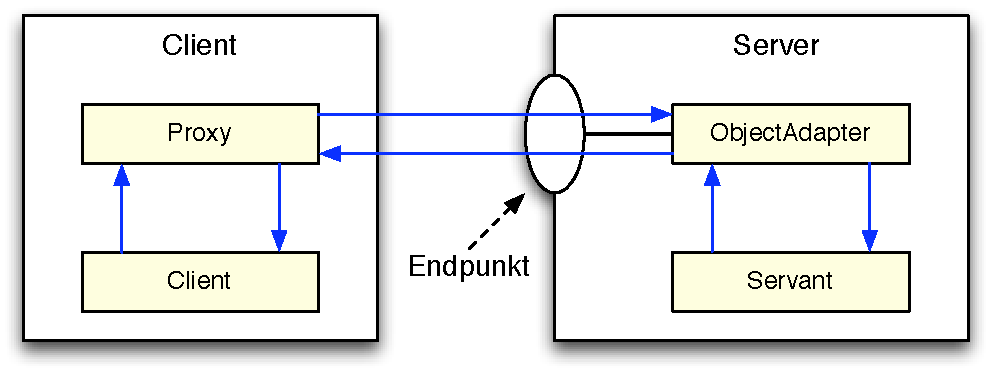
\includegraphics[bb=0bp 0bp 17cm 65mm,clip,scale=0.7]{design_dev/componentmodels/structure}

\caption{\label{fig:ice_structure}Proxystruktur}

\end{figure}


%
\begin{figure}
\centering

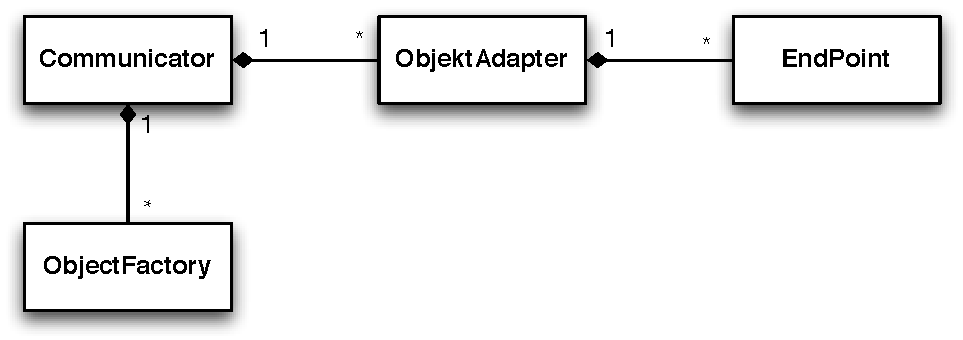
\includegraphics[bb=0bp 0bp 165mm 6cm,clip,scale=0.7]{design_dev/componentmodels/runtime}

\caption{\label{fig:ice_runtime}Objekte zur Laufzeit}

\end{figure}


Ice bietet mehrere verschiedene Arten von Methodenaufrufen an: 
\begin{description}
\item [{synchroner}] Methodenaufruf (synchronous method invocation) entspricht
einem entfernten Funktionsaufruf (siehe Abschnitt \ref{sec:message_types}
$\rightarrow$ remote-invocation send). 
\item [{asynchroner}] Methodenaufruf (asynchronous method invocation) entspricht
einem asynchronen Funktionsaufruf mit callback Modell. F�r den Server
ist der asynchrone Methodenaufruf transparent! ($\rightarrow$ no-wait
send). 
\item [{asynchrone}] Methodenverarbeitung (asychronous method dispatch)
ist das entsprechende Gegenst�ck zum asynchronen Methodenaufruf am
Server. T�tigt der Client einen Methodenaufruf, dann wird der Server
davon benachrichtigt. Im Gegensatz zu einem synchronen Aufruf, der
einen Thread am Server f�r die Abarbeitungszeit des Methodenaufrufes
belegt, kann der Server entscheiden die Anfrage erst zu einem sp�teren
Zeitpunkt zu bearbeiten. Dadurch wird daf�r kein Serverthread belegt.


Sinn macht das, wenn der Server selbst wieder auf das Ergebnis eines
asynchronen Methodenaufrufes warten muss. 

\item [{Einweg}] Methodenaufruf (oneway method invocation) entspricht dem
asynchronen Funktionsaufruf. D.h.~der Methodenaufruf kommt zur�ck,
wenn die Nachricht an das lokale Transportsystem �bergeben worden
ist. So eine Art von Methodenaufrufe sind demzufolge nicht zuverl�ssig.
Da keinerlei R�ckgabe erfolgt, kann diese Art auch keinen R�ckgabewert
besitzen. D.h.~es entspricht einem asynchronen Prozeduraufruf. Einweg
Methodenaufrufe werden nur �ber ein Stream-orientiertes Protokoll
versendet. D.h., dass auf dem �bertragungsweg keine Informationen
verloren gehen k�nnen und auch keine Verf�lschungen auftreten! 
\item [{Serien-Einweg}] Methodenaufruf Wie der vorhergehende Punkt, jedoch
lassen sich mehrere Einweg Methodenaufrufe zu einem Aufruf zusammenfassen,
das eine verbesserte Performanz ergibt. Allerdings werden alle Methodenaufrufe
eines Serien-Einweg Methodenaufrufes am Server in einem Thread abgearbeitet. 
\item [{Datagram}] Methodenaufruf Dies entspricht einem Einweg Methodenaufruf
jedoch mit UDP als Transportprotokoll. Damit sind zus�tzlich zu den
`Nachteilen' des Einweg Methodenaufruf auch noch die Nachteile von
UDP vorhanden. D.h.~einzelne Pakete k�nnen verloren gehen oder doppelt
beim Server ankommen. Daher ist der Haupteinsatz von Datagram Methodenaufrufen
auf das LAN beschr�nkt, wo die Pakete mit hoher Wahrscheinlichkeit
ankommen. 
\item [{Serien-Datagram}] Methodenaufruf analog zum Serien-Einweg Methodenaufruf.
Die Verarbeitung findet am Server wieder in einem Thread statt. 
\end{description}
Bei den synchronen und den asynchronen Methodenaufrufen ist sichergestellt,
dass Ice entweder die Methode zustellt oder eine Fehlermeldung liefert!


\subsection{Dienste}

Ice bietet eine Reihe von Diensten an: 
\begin{description}
\item [{IceGrid}] ein Namensdienst, Serveraktivierung, Softwareverteilung
(in Kombination mit IcePatch2), Replizierung und Load-Balancing, automatisches
`failover', Administration. 
\item [{Freeze}] mit Freeze k�nnen Objekt persistent gemacht werden. 
\item [{IceStorm}] eine einfache Publish/Sucribe MOM 
\item [{IcePatch2}] ein Dienst, um auf Dateien zu replizieren. 
\item [{IceSSL}] Ice �ber SSL transparent verwenden. 
\item [{Glacier2}] ein Firewall Dienst, um Ice durch eine Firewall und
sicher (mittels IceSSL) zu betreiben. 
\item [{IceBox}] ist an sich ein ,,super server'' f�r Ice, sodass server
als Dienst betrieben werden k�nnen. 
\end{description}

\subsection{Slice}

Slice (Specification Language for Ice) ist an sich eine IDL. Genauso
wie CORBA sogenannte Sprachabbildungen (language mappings) definiert,
definiert auch Ice language mappings. In diesem Fall f�r die Programmiersprachen
\texttt{C++}, C\#, Java, Python, VisualBasic und PHP (nur Client).


\subsubsection{Slice Sprache}

Die Syntax sieht fast wie Java aus.
\begin{itemize}
\item Slice Dateien m�ssen mit \texttt{.ice} enden. 
\item Identifier nur aus ASCII Zeichen. Alle Identifier, die mit ,,Ice''
beginnen sind reserviert. Identifier, die mit Helper, Holder, Prx
oder Ptr enden sind ebenfalls nicht erlaubt. Keine underscores! 
\item Alle Identifier sind case-insensitive, m�ssen jedoch konsistent geschrieben
werden. 
\item Kommentare wie in \texttt{C++}. 
\item Es muss immer ein Modul geben. In dieses Modul k�nnen alle Slice Konstrukte
geschrieben werden. Module k�nnen sich �ber mehrere Dateien erstrecken
und werden auf Java packages abgebildet. 
\item An Basisdatentypen gibt es die integralen Datentypen: \texttt{bool}
(false, true), \texttt{byte}, \texttt{short} (16 bits), \texttt{int}
(32 bits), \texttt{long} (64bits) und weiters die nicht integralen
Datentypen \texttt{float} (IEEE single precision, 32 bits), \texttt{double}
(IEEE double precision 64 bits), \texttt{string} (Unicode ohne Nullzeichen).
Alle Zahlen sind wie in Java vorzeichenbehaftet. 
\item Konstanten: \texttt{const double PI = 3.1425926;}
\item enum und struct in etwa wie in \texttt{C++}. Alle enum Konstanten
sind im umschlie�enden Namensraum (ebenfalls wie in \texttt{C++}). 
\item Sequenzen sehen in etwa folgenderma�en aus: \texttt{sequence<Book>
BookLst} 
\item Dictionaries: \texttt{dictionary<string, Book> BookDict} kann z.B.
ein assoziatives Array darstellen, das eine ISBN Nummer mit einem
Buch - Objekt verbindet. Als keys d�rfen auf jeden Fall integrale
Datentypen, Aufz�hlungstypen und string verwendet werden. 
\item Exceptions m�ssen explizit deklariert werden und sind wie structs
anzugeben: \texttt{exception ValveError \{ int valueId; int cause;
\}}
\item Interfaces, Klassen und Methoden werden in etwa wie in Java deklariert,
allerdings ist kein overloading von Methoden erlaubt. 
\item Typdefinitionen d�rfen nicht verschachtelt werden (Ausnahme: Module). 
\item Parameter und Returnwerte werden pass-per-value �bergeben. 
\item Wird ein Parameter mit einem \texttt{{*}} versehen, dann wird der
Parameter als Proxy verstanden. D.h.~von der Semantik her, handelt
es sich um pass-per-reference. 
\item Methoden k�nnen als \texttt{nonmutating} deklariert werden. Im Falle
eines Verbindungsabbruch kann einfach die Methode nochmals gesendet
werden (in \texttt{C++} werden solche Methoden zus�zlich const deklariert). 
\item Methoden k�nnen als \texttt{idempotent} deklariert werden. Dies bedeutet,
dass die Methode mehrmals aufgerufen werden kann und immer das selbe
bewirkt (\texttt{x = 1} ist idempotent). Eine Methode kann allerdings
nicht idempotent und nonmutating gleichzeitig sein (nonmutating impliziert
idempotent). 
\item Forward Declarations sind m�glich! 
\item Der Operator \texttt{::} wird verwendet, um auf Typen in anderen Modulen
zuzugreifen (a la \texttt{C++}). 
\end{itemize}

\subsubsection{Java Mapping}
\begin{itemize}
\item Konstanten werden als Interface mit einer Konstanten names \texttt{value}
abgebildet: \texttt{interface PI \{ value = 3.1415926; \}} 
\item enum und struct werden auf Klassen abgebildet. 
\item Sequenzen werden auf Arrays abgebildet. Es kann jedoch eine alternative
Implementierung folgenderma�en angegeben werden:\\
\texttt{{[}\textquotedbl{}java:type:java.util.LinkedList\textquotedbl{}{]}sequence<Book>
BookLst} 
\item Dictionaries werden immer als eine Instanz vom Typ \texttt{java.util.Map}
dargestellt (defaultm��ig \texttt{java.util.HashMap}). 
\item Exceptions werden als Klasse von der Klasse \texttt{Ice.UserException}
abgeleitet. Wird eine Exception geworfen, die nicht in einer Methode
deklariert ist, dann erh�lt der Client eine Exception, die von \texttt{Ice.LocalException}
abgeleitet ist. 
\item Proxies, Sequenzen, Dictionaries und Strings k�nnen als Parameter
als \texttt{null} �bergeben werden. Allerdings werden immer ,,leere''
Objekte �bertragen. Ein ,,leerer'' Proxy entspricht einem \texttt{null}
Pointer. 
\end{itemize}

\subsection{Programmiermodell}


\minisec{Definition eines Slice Interfaces}


\begin{lstlisting}[language=IDL]
// calculator.ice
module Calculator {
  interface Power {
    double pow(double x, double y);
  };
};
\end{lstlisting}



\minisec{Generieren der Stubs und Skeletons}


\begin{lstlisting}[language=sh]
mkdir generated
slice2java --output-dir generated calculator.ice
\end{lstlisting}


Dabei werden die erzeugten Dateien im Verzeichnis \texttt{generated}
abgelegt.


\minisec{Implementierung der Servant - Klasse}


\begin{lstlisting}
public class SimpleCalculator extends Calculator.PowerDisp {
  public double pow(double x, double y, Ice.Current current) {
    return Math.pow(x,y);
  }
}
\end{lstlisting}


Dinge, die zu beachten sind: 
\begin{itemize}
\item Die Servant-Klasse muss immer von einer bestimmten Klasse abgeleitet
werden. Diese wird von \texttt{slice2java} generiert und befindet
sich in einem Paket, das so hei�t wie der Modulname aus der \texttt{.ice}
Datei. Der Klassenname beginnt mit einem underscore und es wird einfach
`Disp' angeh�ngt. 
\item Als letzter Parameter jeder Methode muss ein zus�tzlicher Parameter
mit dem Typ \texttt{Ice.Current} angeh�ngt werden, der jedoch vorerst
nicht beachtet werden muss. 
\item Der Name der Klasse sollte entweder durch Anh�ngen von ,,I'' (z.B.
\texttt{CalculatorI}, wie Impelementierung) oder durch Angabe einer
speziellen Funktion (wie z.B. \texttt{SimpleCalculator}, d.h. einfache
Implementierung der Schnittstelle Calculator) vorgenommen werden. 
\end{itemize}

\begin{lstlisting}[language=sh]
# oder permanent setzen
export CLASSPATH=classes:CLASSPATH
javac -d classes -source 1.4 generated/Calculator/*.java
javac -d classes SimpleCalculator.java
\end{lstlisting}


Zu beachten ist, dass die Java-Sourcen f�r die Skeletons in Java 1.4
�bersetzt werden m�ssen (die eigenen nicht).


\minisec{Implementierung des Server-Programmes}


\begin{lstlisting}
// von Ice.Application ableiten:
// k�mmert sich um initialisieren und beenden (Communicator Instanz)
// Argumentenliste wird gelesen und Ice Optionen aus args entfernt
// au�erdem wird ein Exception Handler installiert (f�r java.lang.Exception)
public class Server extends Ice.Application {
  // run Methode implementieren
  public int run(String[] args) {

    // liefert eine Referenz auf den Communicator zur�ck
    Ice.Communicator ic = communicator();
    // Anlegen eines Object Adapters mit einem Endpunkt
    Ice.ObjectAdapter adapter =
      ic.createObjectAdapterWithEndpoints("SimpleCalculatorAdapter",
                                          "default -p 10000");

    Ice.Object object = new SimpleCalculator(); // Servant erzeugen

    // Servant beim Adapter registrieren
    adapter.add(object,Ice.Util.stringToIdentity("calculator"));

    adapter.activate(); // aktiviert: dann werden Requests angenommen

    ic.waitForShutdown(); // blockiert bis Server beendet wird

    // wenn shutdown auf Communicator (z.B. Ctrl-C), dann... 
    if (interrupted())
      System.out.println(appName() + ": terminating");

    return 0; // alles ok, beenden
  }

  public static void main(String[] args) {
    // Application instanzieren
    Server app = new Server();
    // ruft die obige run Methode auf und k�mmert sich, dass die
    // Communicator Instanz erzeugt und *sicher* wieder entfernt wird.
    // Application bekommt Name: Server
    int status = app.main("Server", args);
    System.exit(status);
  }
}
\end{lstlisting}


Danach kann man die serverseitigen Klassen kompilieren:


\begin{lstlisting}[language=sh]
javac -d classes Server.java
\end{lstlisting}



\minisec{Implementierung des Client-Programmes}


\begin{lstlisting}
// von Ice.Application ableiten
public class Client extends Ice.Application {
  public int run(String[] args) {
    Ice.Communicator ic = communicator();

    // mache Proxy aus String
    // NAME:PROTOKOLL -p PORT
    Ice.ObjectPrx obj = ic.stringToProxy("calculator:default -p 10000");

    // nachfragen, ob wirklich ein PowerPrx: dazu wird eine Klasse
    // PowerPrxHelper verwendet, die von slice2java erzeugt wird
    // checkedCast ... Server wird nach dem Typ gefragt
    // uncheckedCast ... Server wird nicht gefragt
    Calculator.PowerPrx power = Calculator.PowerPrxHelper.checkedCast(obj);

    if (power == null)
      throw new Error("Invalid proxy");

    System.out.println("2**3= " + power.pow(2,3));
    return 0; // alles ok, beenden
  }

  public static void main(String[] args) {
    Client app = new Client();
    int status = app.main("Client", args);
    System.exit(status);
  }
}
\end{lstlisting}


Danach kann man der Client kompiliert werden:


\begin{lstlisting}[language=sh]
javac -d classes Client.java
\end{lstlisting}



\minisec{Starten von Server und Client}


\begin{lstlisting}
java Server
# und in einer anderen Shell:
java Client
\end{lstlisting}



\subsection{Proxies und Klassen als Parameter und Returnwerte}


\minisec{Proxies als R�ckgabe}

Oft m�ssen Proxies zur�ckgegeben werden. Dazu muss der Server einen
Proxy anlegen.
\begin{enumerate}
\item Entsprechende Slice Definition anlegen, z.B.:\\

\begin{lstlisting}
interface CalcMgr {
  Science* getScienceCalculator();
}
\end{lstlisting}

\item Am Server muss zumindest ein Mal ein Proxy angelegt werden:\\

\begin{lstlisting}
// addWithUUID liefert Typ ObjectPrx deshalb uncheckedCast!
// ist gleich zu `add(object, Ice.Util.generateUUID())'
simpSciencePrx = SciencePrxHelper.
  uncheckedCast(adapter.addWithUUID(new SimpleScience()));
\end{lstlisting}
Von Slice wird automatisch auch eine `Helper' Klasse generiert, die
eine Proxy Instanz erzeugt. Die Methode \texttt{addWithUUID} registriert
einen Servant beim Object Adapter mit einer eindeutigen ID. Da wir
den Proxy zur�ckliefern ist eine allgemein bekannte ID nicht notwendig. 
\end{enumerate}

\minisec{Instanzen von Klassen}

Will man Instanzen von Klassen zur�ckliefern, dann muss die Ice Runtime
wissen, um welche Klasse es sich handelt und wie diese zu instanzieren
ist (verschiedene Programmiersprachen!).

Daf�r wollen wir das vorhergehende Beispiel erweitern. Nehmen wir
dazu an, dass die Berechnung aus Performancegr�nden jetzt am Client
stattfinden soll. Dazu soll der Server einen Taschenrechner �bertragen.
\begin{enumerate}
\item �ndern der Slice Datei: Klassen statt Interface bei den Returnwerten,
also z.B. \texttt{Finance getFinanceCalculator()} wobei \texttt{Finance}
jetzt eine Klasse in der Slice Datei sein soll.


Prinzipiell kann der R�ckgabewert formal auch ein Interface sein.
Es muss lediglich auch eine Klassendeklaration geben, die dieses Interface
auch implementiert, sodass Ice wei� welche Instanzvariablen zu �bertragen
sind. 

\item Der Server ist insoferne anzupassen, dass dieser jetzt direkt Instanzen
dieser Klassen zur�ckliefert anstatt Proxies auf Interfaces.


Unabh�ngig davon macht es u.U. auch Sinn Proxies auf Klasseninstanzen
zur�ckzuliefern. 

\item Es ist eine ObjectFactory zu implementieren, die die Instanzen anlegt:\\

\begin{lstlisting}
class ObjectFactory
  extends Ice.LocalObjectImpl // Achtung: *Local*
  implements Ice.ObjectFactory {

  public Ice.Object create(String type) {
    // Typ von Klasse Science
    // ::                         vom globalen Namensraum ausgehend 
    //   Calculator               zum Calculator Modul
    //             ::Finance      zur Finance Klasse
    if (type.equals("::Calculator::Finance")) {
      return new SimpleFinance();
    } else {
      assert(false);
    }
    return null; 

  public void destroy() {}
}
\end{lstlisting}

\item Jetzt ist nur noch mehr die Factory zu installieren:\\

\begin{lstlisting}
Ice.Communicator ic = communicator();
ObjectFactory of = new ObjectFactory();
ic.addObjectFactory(of, "::Calculator::Finance");
\end{lstlisting}

\end{enumerate}

\subsection{Ice Properties und Konfiguration}

Die Konfigurationsdateien sind einfach aufgebaut:


\begin{lstlisting}[language=sh]
application.category[.subcategory]=value
\end{lstlisting}



\begin{lstlisting}[language=sh]
export ICECONFIG=config ./server
\end{lstlisting}


Die Konfigurationsdatei kann auch �ber die Kommandozeile wie jedes
Property gesetzt werden:


\begin{lstlisting}[language=sh]
./server Ice.Config=config
\end{lstlisting}


Interessant ist das Property \texttt{Ice.Trace.Protocol}, das als
Wert den Level f�r die Ausgabe der Netzwerksmeldungen bekommt. H�chster
Wert ist 3. Sollen keine Meldungen ausgegeben werden, dann ist der
Wert leer zu lassen.


\begin{lstlisting}[language=sh]
./server --Ice.Trace.Protocol=1 # oder ./server --Ice.Trace.Protocol
\end{lstlisting}



%% 
\chapter{Systemarchitektur}


\minisec{Definition}

Es gibt keine allgemein g�ltige Definition des Begriffes `Systemarchitektur'.
Die folgende Definition ist von G.Booch:
\begin{quote}
Die Architektur regelt den konzeptionellen Zusammenhang zwischen den
verschiedenen eigenst�ndigen Komponenten eines Systems. Sie formt
die logische und physikalische Struktur eines Systems mit allen strategischen
und taktischen Entwurfsentscheidungen, welche w�hrend dem Entwicklungsprozess
angewendet werden m�ssen. 
\end{quote}
Das SEI (Software Engineering Institute) der Carnegie Mellon University
definiert den Begriff `architecture' folgenderma�en:
\begin{quote}
A specification that identifies components and their associated functionality,
describes connectivity of components, and describes the mapping of
functionality onto components. Architectures can be of different types,
e.g., hardware, software, or system, and can be domain-specific, e.g.,
networking. 
\end{quote}
Eine etwas pragmatischere Defintion f�r den Begriff Systemarchitektur:
Man versteht darunter die Konzipierung des Aufbaus von IT-Systemen
aus Hardware, System-, Middleware- und Anwendungssoftware, Netzwerkstrukturen,
Betriebspersonal und Nutzern.

Die Systemarchitektur als solches ist ein Produkt (oder auch Artifakt),
das im Zuge der Entwicklung entsteht und der Kommunikation zwischen
den Projektmitgliedern dient.


\minisec{Kriterien f�r eine gute Architektur}
\begin{description}
\item [{Einfachheit}] KISS Prinzip 
\item [{Funktionalit�t}] In welchem Ma�e wird die geforderte Funktionalit�t
abgedeckt? 
\item [{Erweiterbarkeit}] extrem wichtig, besonders im Hinblick auf iterative
Entwicklung 
\item [{Kapselung}] starke Bindung innerhalb der Komponenten, schwache
zwischen den Komponenten 
\end{description}

\minisec{Abgrenzung zur Softwarearchitektur}

W�hrend sich die Systemarchitektur mit dem Aufbau und dem Zusammenspiel
als auch dem Umfeld des gesamten Systems besch�ftigt, hat die Softwarearchitektur
den Aufbau und das Zusammenspiel der Software zum Inhalt.

In der Regel wird die gew�hlte Systemarchitektur einen gro�en Einfluss
auf die Softwarearchitektur haben!

Ohne auf Details eingehen zu wollen, werden wir uns in weiterer Folge
auf die logische Struktur konzentrieren.


\section{Client-Server-Modell}


\subsection{Schichten}

Es gibt (zumindest) \emph{drei unterschiedliche Schichten} in denen
Client- oder Server-Funktionalit�t beinhaltet sein kann:
\begin{itemize}
\item Pr�sentationsebene (Presentation Layer, PL) Darstellung der Daten
und Verarbeitung der Benutzereingaben.

\begin{itemize}
\item zeichenbasierte Benutzeroberfl�che (Mainframe, DOS, Terminal) 
\item graphische Benutzeroberfl�che (Win, X-Windows) 
\end{itemize}
Diese Ebene kann auch noch aufgegliedert werden in:
\begin{itemize}
\item Reine Anzeigefunktionalit�t (View - Komponente des MVC Paradigmas) 
\item Steuerung der Benutzerschnittstelle (Control - Komponente des MVC
Paradigmas, Presentation Logic) 
\end{itemize}
\item Verarbeitungsebene (Application Layer, AL)


Beinhaltet die Business-Logic (Verarbeitung und Auswertung der Daten).

\item Datenebene (Data Layer, DL) 

\begin{itemize}
\item Persistenz der Daten: Dateisystem oder Datenbank 
\item Datenunabh�ngigkeit: Unabh�ngigkeit von den Applikationen soll gegeben
sein. 
\item Datenkonsistenz: DL soll die Konsistenz der Daten sicherstellen k�nnen
(z.B. durch Trigger in RDBMS oder Invarianten in OODBMS). 
\end{itemize}
\end{itemize}

\subsection{Client/Server - Architekturen}

Je nach Aufteilung der Schichtung auf Client bzw. Server entstehen
verschiedene \emph{Client/Server - Architekturen}:
\begin{itemize}
\item 2-Tier 

\begin{itemize}
\item Client: PL --- Server: PL, AL, DL 
\item Client: PL --- Server: AL, DL 
\item Client: PL, AL --- Server: AL, DL 
\item Client: PL, AL --- Server: DL 
\item Client: PL, AL, DL --- Server: DL 
\end{itemize}
PL ... Presentation Layer (Terminal, GUI)\\
 AL ... Application Layer (Business Logic)\\
 DL ... Data Layer (z.B. Dateisystem, XML Datenquellen, Datenbanken)

Je nach Menge der Funktionalit�t am Client spricht man von Thin Client
bzw. von Fat Client.

\item 3-Tier (Server kann auch als Client arbeiten) 

\begin{itemize}
\item Client: PL 
\item Anwendungserver (ist Client von Datenserver): AL 
\item Datenserver: DL 
\end{itemize}
\item n-Tier (weitere Aufteilung um z.B. auch Webclients zu bedienen) 

\begin{itemize}
\item Client: PL (mit Presentation Logic) 
\item Client: PL (ohne Presentation Logic, z.B. Webbrowser, oft hinter einer
Firewall) 
\item Server: PL (beinhaltet Presentation Logic) 
\item Server: AL 
\item Datenserver: DL 
\end{itemize}
n-Tier Architekturen dieser oder �hnlicher Art mit einer Firewall
sind in Firmennetzwerken anzutreffen. Achtung, bei Firewalls treten
die bekannten Probleme meistens an 2 Stellen auf: Einmal auf der Server-Seite
und einmal auf der Client-Seite! 

\end{itemize}
Es ist offensichtlich, dass in jeder Schicht mehrere physische Computer
angesiedelt sein k�nnen, die durchaus auch verschiedene Funktionen
haben k�nnen und unterschiedlich miteinander kooperieren.


\subsection{Kriterien}

Je nach Konfiguration und Anwendung k�nnen verschiede Aspekte zur
Entscheidung �ber eine Architektur betrachtet werden.

Kriterien f�r die Auswahl einer geeigneten Architektur (abgesehen
von den Kriterien, die direkt aus den allgemeinen Zielen abgeleitet
werden k�nnen):
\begin{itemize}
\item Antwortzeitverhalten, Netzwerkbelastung (Durchsatz): abh�ngig von
Netzwerk, Server, Client, Software,... 
\item Zuverl�ssigkeit und Verf�gbarkeit: Redundanz der Daten durch Replikation,
Redundanz der Hardware (Server, Netzwerk), Redundanz in der Software,
Hardwaretausch,... 
\item Sicherheit ($\rightarrow$ Sicherheit) 
\item Integration in Legacy-Systeme: wie l��t sich das neue System in die
bestehenden Systeme integrieren? Import von Daten, Austausch von Daten,
Authentifizierung und Zugriffskontrolle der Benutzer,... 
\item Flexibilit�t: z.B. Austauschbarkeit der Benutzerschnittstelle,... 
\item Installation und Wartbarkeit: Wie leicht l��t sich das System installieren?
Wie leicht kann es gewartet werden? Wie leicht k�nnen neue Versionen
eingespielt werden (Application Deployment)? 
\item Skalierbarkeit: Hardwareaufr�stungen, neue Benutzer 
\item Administration 
\item Programmierproduktivit�t: je nach Komplexit�t der Anforderungen (siehe
Ziele) und der Systemarchitektur sowie der verwendeten Entwicklungstools! 
\item Kosten: von Lizenzen, Eigentumsverh�ltnisse 
\end{itemize}
Als 'Spezialfall' der Client/Server Anordnung, die in dieser Form
als vertikale Anordnung bezeichnet wird, kann die horizontale Anordnung
bezeichnet werden, bei der ein Client oder ein Server in logisch �quivalente
Teile aufgegliedert werden, die jeder mit einem eigenem Anteil der
vollst�ndigen Datenmenge operieren.


\section{Peer-to-Peer Architektur}

F�r bestimmte Arten von Anwendungen kann eine sogenannte Peer-to-Peer
Architektur eingesetzt werden. Das besondere an einer derartigen Architektur
ist, dass es keinen dedizierten Server gibt. In diesem Modell ist
es so, dass z.B. ein Host Kontakt zu einem anderen Host aufnimmt und
diese danach miteinander kommunizieren. Weitere Hosts k�nnen ebenfalls
mit diesen Hosts kommunizieren. D.h.~im Sinne des Client / Server
Konzeptes tauschen Client und Server die Rollen!

Der Vorteil ist, dass nicht ein einzelner Server den Flaschenhals
bildet.

Nachteile sind, dass es schwierig sein kann 
\begin{itemize}
\item einen einheitlichen globalen Status einer Anwendung zu gew�hrleisten. 
\item ein effizientes Routing der Kommunikation sicherzustellen. 
\item einen Kommunikationspartner zu finden. 
\item Netzwerksausf�lle zu maskieren. 
\end{itemize}
Hauptgrund f�r die oben genannten Nachteile ist, dass es keine zentrale
Instanz gibt, die die Aufgaben �bernimmt.

Bekannte Anwendungen der Peer-to-Peer Architektur sind z.B. Chat oder
File-Sharing (Napster, Gnutella).


\section{Push-Architektur}

Das im Internet dominierende Kommunikationsmodell ist das vom WWW
bekannte Request/Reply Schema: ein aktiver Client stellt eine Anfrage
und `pulled' Information vom Server. D.h.~der Client muss wissen
\emph{wo} und \emph{wann} die Information vorhanden ist. Dadurch ist
es die Aufgabe des Benutzers Informationen zu finden und regelm��ig
auf Verf�gbarkeit bzw.~�nderung zu �berpr�fen. Ist ein kontinuierlicher
Informationsfluss notwendig, versagt dieses Kommunikationsmuster (polling!).

Bei der \emph{Push-Architektur} wird die Information ohne Zutun des
Clients vom Server {}``gepushed''. Haupts�chlicher Einsatzzweck
ist es gro�e Mengen von Informationen an eine gro�e Anzahl von Benutzern
zu verteilen. Beispiele daf�r gibt es schon seit den Anf�ngen des
Internet, wie z.B. E-Mail oder Usenet News.

Das allgemeine Modell sieht folgenderma�en aus: Ein Anbieter von Informationen
klassifiziert diese und k�ndigt die Verf�gbarkeit der Informationen
(z.B. als Kanal) an. Interessenten abonnieren beim Anbieter bestimmte
Informationskategorien (also Kan�le). Sobald neue Information vorhanden
ist wird diese an alle Abonnenten verteilt.

Vergleiche entsprechende Implementierungen von MOM, die ebenfalls
diese Funktion anbieten.


\section{Event-Architektur}

Event-basierte Systeme (EBS) sind in gewisser Weise eng verwandt mit
Push-basierten Systemen. Bei diesem Ansatz geht es darum, dass Ereignisse
und deren Verteilung in den Vordergrund gestellt werden.

In einem EBS interagieren die beteiligten, verteilten Komponenten
dadurch, dass sie Events erzeugen und empfangen, ohne dass eine direkte
Verbindung zwischen ihnen besteht. Vielmehr kann jede Komponente Events
erzeugen und and die EBS-Infrastruktur �bergeben, die diese dann verteilt.
Komponenten k�nnen ihr Interesse an bestimmten Events, Event-Klassen
oder auch bestimmten Event-Mustern bei der EBS-Infrastruktur registrieren
und werden benachrichtigt, sobald passende Events oder Muster auftreten.
Ein Beispiel k�nnte sein, dass eine Komponente eines B�rseinformationssystem
informiert werden will, wenn eine Aktie unter einen gewissen Wert
f�llt.

Die Unterschiede zur Push-Architektur liegen darin, dass Events einerseits
prinzipiell kleine Informationsmengen repr�sentieren und dass die
Spezifizierung der gew�nschten Information viel genauer ist.

Ein besondere Herausforderung ist ein effizientes Routing der Events,
insbesondere wenn Muster von Events unterst�tzt werden, da es bei
vielen Komponenten und entsprechender Event-Frequenz schnell zu gro�en
Ressourcenverbrauch kommt.


\section{Agenten-Architektur}

Ein Softwareagent ist ein Computerprogramm, das zielorientiert in
einem dynamischen Umfeld f�r einen Menschen oder eine andere Software
ohne direkte �berwachung m�glichst selbst�ndig Aufgaben l�sen soll.

Folgendes Szeneario will man mit Hilfe einer Agenten-Architektur erreichen:
\begin{quote}
Ein Benutzer will sich eine Reise zusammenstellen und bedient sich
dazu eines Softwareagenten. Unter einem solchen Agenten kann man sich
eine Einheit vorstellen, die f�r den Benutzer die g�nstigste Reiseroute
zusammenstellt (in Bezug auf Zeit, Geld, zur�ckgelegte Strecke) und
den g�nstigsten Reiseveranstalter selbst�ndig ausfindig macht. Dazu
bekommen sie vom Benutzer die Vorgaben bez�glich Reisezeit, Budget,
notwendige Zwischenstopps,... und ermittelt selbst�ndig eine m�glichst
optimale L�sung. Dazu kann sie bei Reiseveranstaltern, Datenbanken,...
Anfragen stellen oder auch andere Agenten um Hilfe bitten. Unter Umst�nden
ist es notwendig, dass sich der Agent auch zu anderen Rechner verschiebt
und zum Schluss mit der L�sung wieder zum Benutzer zur�ckkehrt (z.B.
damit Bandbreite gespart wird). 
\end{quote}
Um die Verschiebbarkeit der Agenten realisieren zu k�nnen ben�tigt
man das Konzept der Code-Migration, das im nachsten Abschnitt besprochen
wird. Danach wird auf die eigentlichen Softwareagenten etwas genauer
eingegangen.


\subsection{Code-Migration}

Zur Erreichung einer Migrationstransparenz bzw.~einer Relokationstransparenz
auf Ausf�hrungsebene, m�ssen auch Threads bzw.~Prozesse von einer
Maschine zu einer anderen Maschine verschoben werden k�nnen.

Um dies durchf�hren zu k�nnen, muss das System eine M�glichkeit der
Code-Migration zur Verf�gung stellen.

Gr�nde in einer erw�nschten Code-Migration liegen meistens darin,
dass die allgemeine Systemleistung verbessert werden soll, z.B.:
\begin{itemize}
\item Code soll immer auf der Client-Maschine ausgef�hrt werden (z.B. Applet). 
\item eine Maschine ist ausgelastet, eine andere Maschine soll �bernehmen. 
\item die Netzwerksbandbreite ist ausgesch�pft. 
\item Der Code soll in die physische N�he der Daten transportiert werden
(um wiederum den Netzwerksoverhead zu minimieren). 
\end{itemize}
Aber auch die Flexibilit�t ist ein Grund f�r den Wunsch den Code an
beliebigen Stellen zur Ausf�hrung zu bringen: Am Client kann dynamisch
eine Konfiguration durchgef�hrt werden!

Grunds�tzlich m�ssen die Maschinen zwischen denen eine Code-Migration
stattfinden entweder:
\begin{itemize}
\item auf der Ebene der Plattform (Hardware, Betriebssystem) eine gemeinsame
Basis aufweisen, oder 
\item eine Ebene mit Zwischencode existieren, mit der plattform�bergreifend
agiert werden kann (Java, C\#, Perl, Python, Ruby, Tcl) oder die Programmiersprache
ist eine reine Interpretersprache, sodass der Quellcode transferiert
wird. 
\end{itemize}
Prinzipiell werden wir nur zwischen zwei Arten der Code-Migration
unterscheiden (obwohl vielf�ltige und feine Unterscheidungen m�glich
sind):
\begin{itemize}
\item schwache Mobilit�t: Es wird nur das Codesegment �bertragen (eventuell
mit Initialisierungsdaten). Deshalb wird bei dieser Art der Mobilit�t
ein �bertragener Code immer von seinem Ausgangsstatus aus gestartet
(z.B. Java Applet). 
\item starke Mobilit�t: Im Gegensatz zur schwachen Mobilit�t wird zus�tzlich
zum Codesegment auch das Ausf�hrungssegment �bertragen. Das charakteristische
Merkmal der starken Mobilit�t ist, dass ein ausgef�hrter Prozess unterbrochen,
auf eine andere Maschine verschoben und dann fortgesetzt werden kann.


Ein spezielles Problem, das haupts�chlich bei der starken Mobilit�t
auftritt ist: Was passiert mit den Ressourcen auf die der Thread zugreift?
Eine offene Datei kann nicht bewegt werden und auch Hardware kann
nicht �ber das Netz verschoben werden. 

\end{itemize}
Besonderes Augenmerk: Sicherheit!


\subsection{Softwareagenten}

\label{sec:sw-agent}

Software-Agenten sind ein Beispiel, wo u.U. Code-Migration auftritt.

Agenten spielen im Kontext verteilter Systeme eine immer wichtiger
werdende Rolle. Es handelt sich dabei um autonome Einheiten, die in
Zusammenarbeit mit anderen (u.U. entfernten) Agenten eine Aufgabe
l�sen.

Allen Softwareagenten ist gemein, dass sie die folgenden Eigenschaften
aufweisen. Sie sind: 
\begin{itemize}
\item autonom: kann eigenst�ndig agieren. 
\item reaktiv: reagiert rechtzeitig auf �nderungen in seiner Umgebung. 
\item proaktiv: initiiert Aktionen, die seine Umgebung beeinflussen. 
\item kommunikativ: kann Informationen mit Benutzern und anderen Agenten
austauschen. 
\end{itemize}
Agenten k�nnen auch noch folgende Eigenschaften aufweisen: 
\begin{itemize}
\item mobil: kann von einem System auf ein anderes migrieren. 
\item adaptiv: ist lernf�hig. Oft handelt es sich dabei um Systeme, die
den Endbenutzer helfen sollen, eine oder mehrere Applikationen zu
benutzen. Solche Agenten sind lernf�hig: je l�nger ein Benutzer mit
dem Agenten arbeitet, desto besser kann der Agent dem Benutzer helfen: 

\begin{itemize}
\item Ein Agent, der K�ufer und Verk�ufer zusammenbringen soll, erkennt
bevorzugte Suchanfragen, Vorlieben,... 
\item Ein E-Mail-Agent kann in der Lage sein, unerw�nschte E-Mail aus der
Mailbox entfernen, oder automatisch in die entsprechenden themenspezifizschen
Mailboxen verteilen. 
\end{itemize}
\end{itemize}



%% 
\chapter{Webservices}


\section{�berblick\label{sec:webservices_overview}}


\minisec{Definition}

Web Services erm�glichen Abwicklungen von Dienstleistungen und Gesch�ften
�ber das Internet. Im engeren technischen Sinn (siehe auch http://www.w3.org/2002/ws)
bedeutet das ein automatisierte Kommunikation zwischen Applikationen
�ber das Internet. Es werden also nicht HTML-Seiten zu einem Webbrowser
geschickt, die von einem Menschen betrachtet werden, sondern Programme
tauschen Daten aus und starten auf entfernten Rechnern Funktionen
(Remote Procedure Call).

\emph{Webservices} sind Dienste, 
\begin{itemize}
\item die im Internet angeboten werden 
\item die standardisierte XML Nachrichten verwenden 
\item die plattform�bergreifend und unabh�ngig von der Programmiersprache
sind. 
\end{itemize}
Zus�tzlich sind zwei weitere Eigenschaften w�nschenswert: 
\begin{itemize}
\item Ein Webservice sollte \emph{selbstbeschreibend} sein, sodass andere
Anwendungen wissen wie sie das Webservice aufrufen k�nnen. Auch eine
f�r Menschen lesbare Beschreibung ist sinnvoll. D.h.~es gibt eine
�ffentliche Schnittstelle, die aus einer f�r Menschen lesbaren Dokumentation
besteht und einer XML Schnittstelle, die die Funktionen, Argumente
und R�ckgabewerte beschreibt. 
\item Ein Webservice sollte \emph{gefunden} werden k�nnen. Dazu muss es
f�r den `Service Provider' eines Dienstes m�glich sein, ein Web-Service
in einer `Service Registry' zu registrieren. Weiters muss ein potentieller
`Service Requestor' das Service finden und danach aufrufen k�nnen. 
\end{itemize}
Damit dieses Ziel erreicht wird, bauen Webservices auf einer Reihe
von Standards und Spezifikation wie XML, SOAP, XML-RPC, WSDL und UDDI
auf.

SOAP, WSDL und UDDI wird intensiv von Microsoft in ihrer .NET Plattform
eingesetzt bzw.~sind fester Bestandteil der J2EE von Sun.


\minisec{Ablauf}

Nehmen wir an, dass wir ein Reisebuchungssystem entwickeln wollen
und dieses System dem Benutzer auch Wetterinformationen zu einem beliebigen
Ort auf der Welt bereitstellen soll.
\begin{enumerate}
\item Der Benutzer dieses Reisebuchungssystem gibt einen Ort (z.B. Peking)
ein. Das System kontaktiert daraufhin ein zentralisiertes Verzeichnis
von Webservices: `Ben�tige Wetterinformation von Peking'. Das Verzeichnis
antwortet mit Informationen �ber ein Webservice (von Peking) und liefert
eine URL auf eine Servicebeschreibung zur�ck. 
\item Jetzt kann die Servicebeschreibung geladen werden (via der angegebenen
URL). 
\item Danach wei� der Client wie er das Webservice aufrufen kann und f�hrt
den Aufruf durch. 
\end{enumerate}

\minisec{Rollen}

Prinzipiell gibt es folgende Rollen: 
\begin{description}
\item [{Service}] provider stellt das Webservice zur Verf�gung. 
\item [{Service}] requestor ist der Konsument des Webservice. 
\item [{Service}] registry ist das logisch zentralisierte Verzeichnis der
Webservices. 
\end{description}

\minisec{Protokollstack}
\begin{description}
\item [{Discovery}] ist zust�ndig f�r das Publizieren und Finden von Webservices.
Diese Funktion wird von UDDI �bernommen. 
\item [{Description}] ist zust�ndig f�r das Beschreiben eines Webservice.
Dies wird von WSDL �bernommen. 
\item [{XML}] messaging ist f�r das �bertragen der XML Nachrichten zust�ndig.
Dies wird durch SOAP bzw.~XML-RPC und XML �bernommen. 
\item [{Transport}] ist das Transportprotokoll. Meistens http, aber auch
smtp, ftp oder beep w�re m�glich. 
\end{description}

\minisec{Programmiermodell}

Client-seitig sind folgende Schritte notwendig:
\begin{enumerate}
\item Finde das Service mittels UDDI 
\item Lade WSDL Dokument (oder XML-RPC Anweisungen) 
\item Erzeuge SOAP (oder XML-RPC) Client 
\item Rufe Webservice auf 
\end{enumerate}
Server-seitig sind folgende Schritte notwendig:
\begin{enumerate}
\item Implementiere Funktionalit�t des Webservice 
\item Implementiere SOAP (oder XML-RPC) Wrapper 
\item Erzeuge WSDL Dokument 
\item Installieren des Webservice 
\item Registrieren mittels UDDI 
\end{enumerate}

\section{XML Programmierung}

Das wahrscheinlich wichtigste Einsatzgebiet von XML liegt in der plattform�bergreifenden
M�glichkeit zur Kommunikation in einem verteilten System. XML wird
auch sehr oft zur Konfiguration von Systemen eingesetzt oder es gibt
auch vermehrte Anwendung in Datenbanksystemen.

\emph{Gr�nde} liegen einerseits in der relativ einfachen Programmierung
von XML Anwendungen, der M�glichkeit plattform�bergreifend Daten auszutauschen
und auch darin, dass das Format von einem Menschen gelesen und auch
ge�ndert werden kann.


\subsection{�berblick}

Es gibt an sich \emph{5 Programmierstile} zur Programmierung mit XML:
\begin{description}
\item [{Push-Stil}] Ein \emph{Push - Modell} ist ein Streaming-API: der
Parser �bernimmt die Kontrolle, liest das Dokument und teilt der Anwendung
mit welche XML Teile erkannt werden. D.h., dass ein Start-Tag, ein
Ende-Tag, Inhalt, Attribute,... im XML-Dokument vorhanden sind. Es
wird auch als \emph{event-basierter} Stil bezeichnet, da Event-Handler
Methoden registriert werden, die im Sinne eines Callback vom Parser
beim Auftreten eines Starttags, eines Attributs,... aufgerufen werden.


\emph{Vorteile} sind, dass solche Parser 
\begin{itemize}
\item relativ einfach zu implementieren sind 
\item sehr schnell und effizient sind 
\item nicht das ganze Dokument auf einmal lesen m�ssen und daher der Speicherplatzbedarf
gering ist. 
\end{itemize}
H�ufig eingesetzt werden diese Art von Parser in Netzwerkanwendungen,
die einen Stream von XML Daten verarbeiten m�ssen.

Ein \emph{Nachteil} ist, dass die Programmierung nur f�r bestimmte
Arten von XML-Dokumenten wirklich einfach ist. Z.B. wenn das XML-Dokument
eine Liste von tausenden Bestellungen beinhaltet, ist dieser Stil
sehr gut geeignet, aber bei komplexen Dokumenten mit Eintr�gen, die
sich u.U. noch aufeinander beziehen, nicht.

Auf Grund der event-basierten Verarbeitung ergibt sich jedoch noch
ein Nachteil, die diesen Ansatz nicht f�r alle Anwendungen geeignet
machen: Das XML Dokukument kann nicht ver�ndert werden. Ist dies gew�nscht,
dann muss z.B. auf einen Vertreter des Baum-basierten Stiles zur�ckgegriffen
werden.

Der wichtigster Vertreter dieses Stiles ist SAX (Simple API for XML,
http://www.sax-project.org). 

\item [{Pull-Stil}] Der \emph{Pull-Stil} ist ebenfalls ein Streaming -
API, aber die Kontrolle liegt nicht mehr beim Parser sondern bei der
XML Anwendung. D.h.~die XML Anwendung fordert beim Parser immer die
n�chste Information an. Derzeit sind Parser dieses Stiles nicht besonders
weit vertreten.


StAX (Streaming API for XML) ist ein Vertreter dieses Stiles. 

\item [{Baum-basierter~Stil}] Das gesamte Dokument beim \emph{baum-basierten
Stil} wird eingelesen und im Speicher als Baumstruktur von Objekten
abgelegt. Die XML Anwendung kann danach durch den Baum navigieren
und diesen ver�ndern. Dieser Stil wird derzeit sehr oft verwendet.


\emph{Vorteil} dieses Stiles ist haupts�chlich die einfache Handhabung
und der gr��te \emph{Nachteil} liegt im Speicherbedarf gro�er XML
Dokumente, da das gesamte Dokument im Hauptspeicher abgelegt wird.

Vertreter dieses Stiles sind das DOM Model (XML Teil) des W3C, dom4j
(http://dom4j.org) und JDOM (http://www.jdom.org) oder XOM (http://www.xom.nu). 

\item [{Daten-basierter~Stil}] Der \emph{daten-basierte} Stil ist dem
baum-basierten Stil �hnlich, jedoch gibt es anstatt den generischen
Knoten spezielle Klassen f�r den jeweiligen Knotentyp. D.h.~anstatt
einer Klasse \texttt{Element} wird bei dem Element \texttt{Buch} eine
entsprechende Klasse \texttt{Buch} verwendet. Diese Zuordnung von
XML-Element zu Klasse wird meistens mittels einer DTD oder eines XML
Schemas vorgenommen.


Neben dem offensichtlichen Vorteil ist der Hauptnachteil dieser Variante,
dass eine Notwendigkeit f�r eine DTD oder ein XML Schema gegeben ist!

Vertreter dieses Stiles ist JAXB (Java Architecture for XML Binding)
von Sun. 

\item [{Abfragestil}] Dazu wird das XML-Dokument meistens mit XPath abgefragt
oder mittels XSLT transformiert. Dieser Stil ist nicht weit verbreitet. 
\end{description}
In weiterer Folge werden die wichtigsten APIs vorgestellt. Dies betrifft
SAX und DOM. Da es sich bei SAX und DOM nur um Spezifikationen und
nicht um Software handelt, gibt es auch verschiedene Implementierungen
daf�r. Jede Implementierung bedingt in der Regel auch verschiedene
Klassennamen bzw.~Packagenamen f�r die Parserklasse und damit auch
eine verschiedene Instanzierung. Um eine einheitliche und portable
Instanzierung zu gew�hrleisten hat Sun ein eigenes API definiert,
das es erm�glicht verschiedene Implementierungen portabel in das Programm
einzubinden. Dieses API nennt sich Java API for XML Processing (JAXP).
In den folgenden Beschreibungen und Beispielen wird JAXP verwendet.


\section{XML-RPC\label{sec:XML-RPC}}

\emph{XML-RPC} existiert ca.~seit 1998 und wird h�ufig im Internet
verwendet. Es wird haupts�chlich eingesetzt, um Webservices zu betreiben
(wie z.B. auch von Google). Es gibt ca.~80 Implementierungen dieses
Protokolls, u.a.~auch f�r Java, C, \texttt{C++}, C\#, Perl, Python,
Ruby. XML-RPC ist allerdings \emph{kein} offizieller Standard, sondern
wurde von der Fa.~UserLand entworfen und und von dieser auch erstmalig
implementiert. Die XML-RPC Homepage ist http://www.xmlrpc.com.

Es geht dazu einen ganz anderen Ansatz als ONC-RPC: es kodiert die
Funktionsaufrufe in XML und verschickt diese mittels http und der
POST Methode. D.h.~die Daten werden nicht bin�r kodiert sondern als
Zeichen (z.B. UTF-8 oder iso-8859-1) �bertragen. Dadurch handelt es
sich nat�rlich auch um ein plattformunabh�ngiges Protokoll.

Wieso wird das so gel�st? Dazu gibt es zumindest zwei Gr�nde:
\begin{itemize}
\item http schafft keine Probleme beim Durchgang durch Firewalls. 
\item XML ist ein Standard, der wirklich unabh�ngig von der Plattform ist. 
\end{itemize}
Eine Beispielanfrage kann so aussehen:


\begin{lstlisting}[language=XML]
<?xml version="1.0" encoding="iso-8859-1"?>
<methodCall>
  <methodName>weather.getTemperature</methodName>
  <params>
    <param><value>Wr. Neustadt</value></param>
  </params>
</methodCall>
\end{lstlisting}


Als Antwort k�nnte zur�ckkommen:


\begin{lstlisting}[language=XML]
<?xml version="1.0" encoding="iso-8859-1">
<methodResponse>
  <params>
    <param><value><int>35<int></value></param>
  </params>
</methodResponse>
\end{lstlisting}


Man sieht, dass der Aufbau sehr einfach ist. XML-RPC l�sst sich weiter
so charakterisieren: 
\begin{itemize}
\item Nur primitive Datentypen, aber auch Arrays und Strukturen. An primitiven
Datentypen gibt es lediglich int, double, Boolean, string, dateTime.iso8601
und base64. Keine Objekte! 
\item kein zustandsorientiertes Protokoll. Es ist nat�rlich m�glich, Zustandsinformationen
als Parameter mitzugeben, wie dies im Prinzip bei der klassischen
Webentwicklung z.B. durch Cookies realisiert wird. 
\item Kein Konzept von Exceptions; jedoch kann ein Webservice einen Fehlercode
und eine Fehlerbeschreibung zur�ckliefern. 
\end{itemize}
Der Hauptgrund in der Verwendung von XML-RPC liegt in der Einfachheit.
Damit lassen sich schnell und unkompliziert Webservices entwickeln.
Ohne den Overhead von UDDI und WSDL, aber auch ohne deren Vorteile!


\minisec{Beispiel: Berechnung der Potenz in Python}

Der Server sieht in Python folgenderma�en aus:


\begin{lstlisting}[language=Python]
import SimpleXMLRPCServer

server = SimpleXMLRPCServer.SimpleXMLRPCServer(("localhost",8000))
server.registerfunction(pow)

print "Ab jetzt werden Anfragen entgegengenommen"
print "Programm mittels Ctrl-C stoppen"

server.serveforever()
\end{lstlisting}


Und dazu der dazugeh�rige Client:


\begin{lstlisting}
import xmlrpclib

server = xmlrpclib.ServerProxy("localhost:8000")
print "2 ** 3 =", server.pow(20,2)
\end{lstlisting}



\minisec{Beispiel: Berechnung der Potenz in Java}

Der Server in Java sieht folgenderma�en aus:


\begin{lstlisting}
// in einer Datei PowerHandler.java
// das ist die eigentliche Serverfunktion
public class PowerHandler {
  public double pow(double x, double y) {
    return Math.pow(x, y);
  }
}

// in einer Datei PowerServer.java
import java.io.IOException;
import org.apache.xmlrpc.WebServer;
import org.apache.xmlrpc.XmlRpc;

public class PowerServer {
  public static void main(String[] args) {
    // verwende internen http Server; Port 8000
    WebServer server = new WebServer(8000);

    server.start(); // starten in eigenem Thread
    server.addHandler("power", new PowerHandler());

    System.out.println("Ab jetzt werden Anfragen entgegengenommen");
    System.out.println("Programm mittels Ctrl-C stoppen");
  }
}
\end{lstlisting}


Und jetzt der Client:


\begin{lstlisting}
mport java.io.IOException;
import java.util.Vector;
import org.apache.xmlrpc.XmlRpcClient;
import org.apache.xmlrpc.XmlRpcException;

public class PowerClient {
  public static void main(String[] args) 
    throws IOException, XmlRpcException {

    try {
      XmlRpcClient client = new XmlRpcClient("http://localhost:8000");

      Vector params = new Vector();
      params.addElement(new Double(2));
      params.addElement(new Double(3));

      Object result = client.execute("power.pow", params);

      String resultStr = result.toString();
      double res = Double.parseDouble(resultStr);

      System.out.println("2 ** 3 = " + res);
    } catch (XmlRpcException e) {
      e.printStackTrace(); // reicht zum Testen
    } catch (IOException e) {
      e.printStackTrace(); // reicht zum Testen
    }
  }
}
\end{lstlisting}



\section{SOAP\label{sec:SOAP}}

\emph{SOAP} (fr�her Simple Object Access Protocol) basiert wie XML-RPC
ebenfalls auf XML, ist ebenfalls ein purer RPC (d.h.~keine entfernte
Objektaufrufe), hat jedoch andere Perspektiven und geht weit �ber
die M�glichkeiten von XML-RPC hinaus:
\begin{itemize}
\item Es wurde prim�r entwickelt, um Web-Services im gro�en Umfeld einzusetzen.
Dazu wurde die Verwendung von XML Namespaces eingesetzt (Namensgleichheit!).
Die Nachrichten sind (hiermit) komplizierter als bei XML-RPC. 
\item Es gibt viel mehr primitive Datentypen als in XML-RPC, wie z.B. unsigned-Varianten
der ganzen Zahlen, positive und nicht positive Zahlen, mehrdimensionale
Arrays,... 
\item SOAP wurde von Anfang mit dem Gedanken entworfen auch andere Transportprotokolle
zu nutzen, wie z.B. FTP, E-Mail,... auch wenn diese de facto nicht
genutzt werden. 
\end{itemize}
Der Weg eines Service Requesters folgenderma�en aus:
\begin{enumerate}
\item Service via UDDI finden. 
\item WSDL Datensatz oder XML-RPC Instruktionen herunterladen. 
\item XML-RPC oder SOAP Client erzeugen. 
\item Service aufrufen. 
\end{enumerate}
Ein Service Provider muss so vorgehen:
\begin{enumerate}
\item Funktionalit�t z.B. mittels EJB oder COM oder .NET entwickeln. 
\item Wrapper entwickeln, z.B. SOAP oder XML-RPC. 
\item WSDL Datensatz oder XML Instruktionen schreiben. 
\item Service installieren. 
\item Service via UDDI registrieren: 'UDDI cloud services' werden von Microsoft
und IBM zur Verf�gung gestellt. Das ist ein logisch zentralisiertes,
aber physikalisch per Replikation dezentralisiertes Verzeichnis (http://www.uddi.org/register). 
\end{enumerate}
SOAP Nachrichten sind komplex und die Generierung von Stubs und Skeletons
wird in der Regel mit Tools durchgef�hrt.

Eine Beispielanfrage kann folgenderma�en aussehen:


\begin{lstlisting}
<?xml version="1.0" encoding="UTF-8"?>
<env:Envelope
  xmlns:env="http://www.w3.org/2003/05/soap/envelope/"
  xmlns:xsi="http://www.w3.org/2001/XMLSchema-instance"
  xmlns:xsd="http://www.w3.org/2001/XMLSchema">
  <env:Body>
    <ns1:getTemperature
      xmlns:ns1="urn:xmethods-Temperature"
      env:encodingStyle="http://www.w3c.org/2003/05/soap/encoding/">
      <zipcode xsi:type="xsd:string">2700</zipcode>
    </ns1:getTemperature>
  </env:Body>
</env>
\end{lstlisting}


und die entsprechende Antwort so:


\begin{lstlisting}
<?xml version="1.0" encoding="UTF-8"?>
<env:Envelope
  xmlns:env="http://www.w3.org/2003/05/soap/envelope/"
  xmlns:xsi="http://www.w3.org/2001/XMLSchema-instance"
  xmlns:xsd="http://www.w3.org/2001/XMLSchema">
  <env:Body>
    <ns1:getTemperatureResponse xmlns:ns1="urn:xmethods-Temperature"
      env:encodingStyle="http://www.w3c.org/2003/05/soap/encoding/">
      <return xsi:type="xsd:float">35</return>
    </ns1:getTemperatureResponse>
  </env:Body>
</env>
\end{lstlisting}


Die Implementierung von SOAP Aufrufen h�ngt stark von der verwendeten
Technologie ab. Im Prinzip folgt sie nat�rlich der Art wie sie auch
bei XML-RPC verwendet wird. Meistens gibt es Tools, die Stubs und
Skeletons generieren und die Programmierung unterst�tzen. In der Regel
werden SOAP Webservices in einem Application Server gehostet.


\section{WSDL\label{sec:wsdl}}

Um die gew�nschte unabh�ngige Beschreibung zu erreichen, besteht eine
WSDL Beschreibung eines Web-Services aus: 
\begin{itemize}
\item einer Schnittstellenbeschreibung aller verf�gbaren Funktionen samt
der Parameter- und R�ckgabewertbeschreibungen. 
\item Angaben �ber das verwendete Transportprotokoll (z.B. SOAP �ber http). 
\item Adresse, unter der das Service aufzurufen ist. 
\end{itemize}
WSDL wird haupts�chlich (aber nicht ausschlie�lich) verwendet um SOAP
Dienste zu beschreiben.

WSDL Nachrichten sind folgenderma�en aufgebaut:
\begin{itemize}
\item Das Wurzelelement ist \texttt{definitions}, das alle anderen Elemente
beinhaltet und auch die Namespaces definiert. 
\item Das \texttt{types} Element wird zum Definieren der Datentypen, die
zwischen Client und Server ben�tigt werden herangezogen. Prinzipiell
werden die Datentypen mit XML Schema spezifiziert. Werden nur die
XML Schema eingebauten einfachen Typen ben�tigt, dann wird das \texttt{types}
Element nicht ben�tigt. 
\item Es k�nnen mehrere \texttt{message} Elemente vorkommen, die jeweils
eine one-way Nachricht angeben (entweder eine Anfrage oder eine Antwort).
So ein \texttt{message} Element definiert den Namen der Nachricht
und kann mehrere \texttt{part} Elemente beinhalten, die entweder die
Parameter der Nachricht oder die Return Werte spezifizieren. 
\item Das \texttt{portType} Element kombiniert ein oder zwei \texttt{message}
Elemente zu einer vollst�ndigen one-way oder request-response Operation.
Dazu wird das \texttt{operation} Element verwendet.


Weitere Arten von Operationen sind die Gegenteile der obigen: solicit-response:
Service sendet eine Nachricht und empf�ngt eine Antwort und notification:
Service sendet eine Nachricht. 

\item \texttt{binding} beschreibt wie eine oder mehrere Operationen versendet
werden. Es handelt sich hierbei in der Regel um die konkreten Daten
f�r die SOAP Dienste (aber auch HTTP GET oder HTTP POST ist gebr�uchlich).
F�r einen portType kann es mehrere bindings geben. 
\item Das \texttt{service} Element definiert die Adresse unter der das Service
erreichbar ist. 
\end{itemize}
Zus�tzlich gibt es noch ein \texttt{documentation} und \texttt{import}
Element.


\begin{lstlisting}[language=XML]
<?xml version="1.0" encoding="UTF-8"?>
<!-- Dokument muss nicht unter www.htlwrn.ac.at/wsdl... zu finden sein -->
<definitions name="HelloService"
  targetNamespace="http://www.htlwrn.ac.at/wsdl/HelloService.wsdl"
  xmlns="http://schemas.xmlsoap.org/wsdl/"
  xmlns:soap="http://schemas.xmlsoap.org/wsdl/soap/"
  xmlns:tns="http://www.htlwrn.ac.at/wsdl/HelloService.wsdl"
  xmlns:xsd="htp://www.w3.org/2001/XMLSchema">

  <!-- Funktionsaufruf besteht aus 2 Nachrichten: -->
  <message name="HelloRequest">    <!-- hin -->
    <part name="firstName" type="xsd:string"/>
  </message>

  <message name="HelloResponse"> <!-- und retour -->
    <part name="greeting" type="xsd:string"/>
  </message>

  <!-- Funktion besteht aus Nachricht hin und wieder zur�ck -->
  <portType name="HelloPortType">
    <operation name="Hello">
      <input message="tns:HelloRequest"/>
      <output message="tns:HelloResponse"/>
    </operation>
  </portType>

  <!-- wir verwenden 'nat�rlich' SOAP -->
  <binding name="HelloBinding" type="tns:HelloPortType">
    <soap:binding style="rpc"
                  transport="http://schemas.xmlsoap.org/soap/http"/>
    <operation name="Hello">
    <soap:operation soapAction="Hello"/>
      <input>
        <soap:body
          encodingStyle="http://schemas.xmlsoap.org/soap/encoding/"
          namespace="urn:examples:helloservice" use="encoded"/>
      </input>
      <output>
        <soap:body
          encodingStyle="http://schemas.xmlsoap.org/soap/encoding/"
          namespace="urn:examples:helloservice" use="encoded"/>
      </output>
    </operation>
  </binding>

  <service name="HelloService">
    <documentation>WSDL File for HelloService</documentation>
    <port binding="tns:HelloBinding" name="HelloPort">
      <soap:address
        location="http://localhost:8080/soap/servlet/rpcrouter"/>
    </port>
  </service>
</definitions>
\end{lstlisting}



\section{UDDI\label{sec:uddi}}

UDDI kann Informationen �ber die Firmen (allg.~Organisation) und
die angebotenen Dienste verwalten und besteht aus zwei Teilen: Der
Spezifikation, um ein verteiltes Verzeichnis f�r Organisationen und
Dienste zu erstellen und einer UDDI Business Registry (UDDI `cloud
service'), die diese Spezifikation umsetzt.

Daten, die verwaltet werden sind: 
\begin{description}
\item [{White}] pages Allgemeines �ber eine Organisation: Name, Beschreibung,
Kontaktinformationen,... 
\item [{Yellow}] pages Klassifikation der Organisationen bzw.~der Dienste.
Z.B. Einteilung nach Industrie, Produkt oder geographischem Standort. 
\item [{Green}] pages Technische Informationen �ber ein Webservice. Also
zum Beispiel die Spezifikation eines Webservice und seine Adresse. 
\end{description}
Der prinzipielle Ablauf der Verwendung von UDDI ist schon in Abschnitt
\ref{sec:webservices_overview} beschrieben.

Technisch gesehen besteht UDDI aus 3 Teilen: 
\begin{description}
\item [{UDDI}] data model Das ist ein XML Schema, um Organisationen und
Dienste zu beschreiben. D.h.~es werden die Informationen haupts�chlich
in businessEntity und businessService eingeteilt. Zus�tzlich gibt
es noch Daten, die angeben wo und wie auf ein Webservice zugegriffen
werden kann 
\item [{UDDI}] API Dabei handelt es sich um ein API, das mittels SOAP beschrieben
ist und zum Suchen und Ver�ffentlichen von UDDI Daten dient. Zus�zlich
k�nnen diese Operationen meistens auch �ber ein Webinterface genutzt
werden. 
\item [{UDDI}] cloud services Die eigentliche `Implementierung' von UDDI
wie oben beschrieben. 
\end{description}


\end{document}
